\chapter{Loglinear and logit models}\label{ch:loglin}
\begin{center}
 \rule[-4pt]{0.5pt}{4pt}\hrulefill\rule[-4pt]{0.5pt}{4pt}\\
 \begin{minipage}[c]{.33\linewidth}
  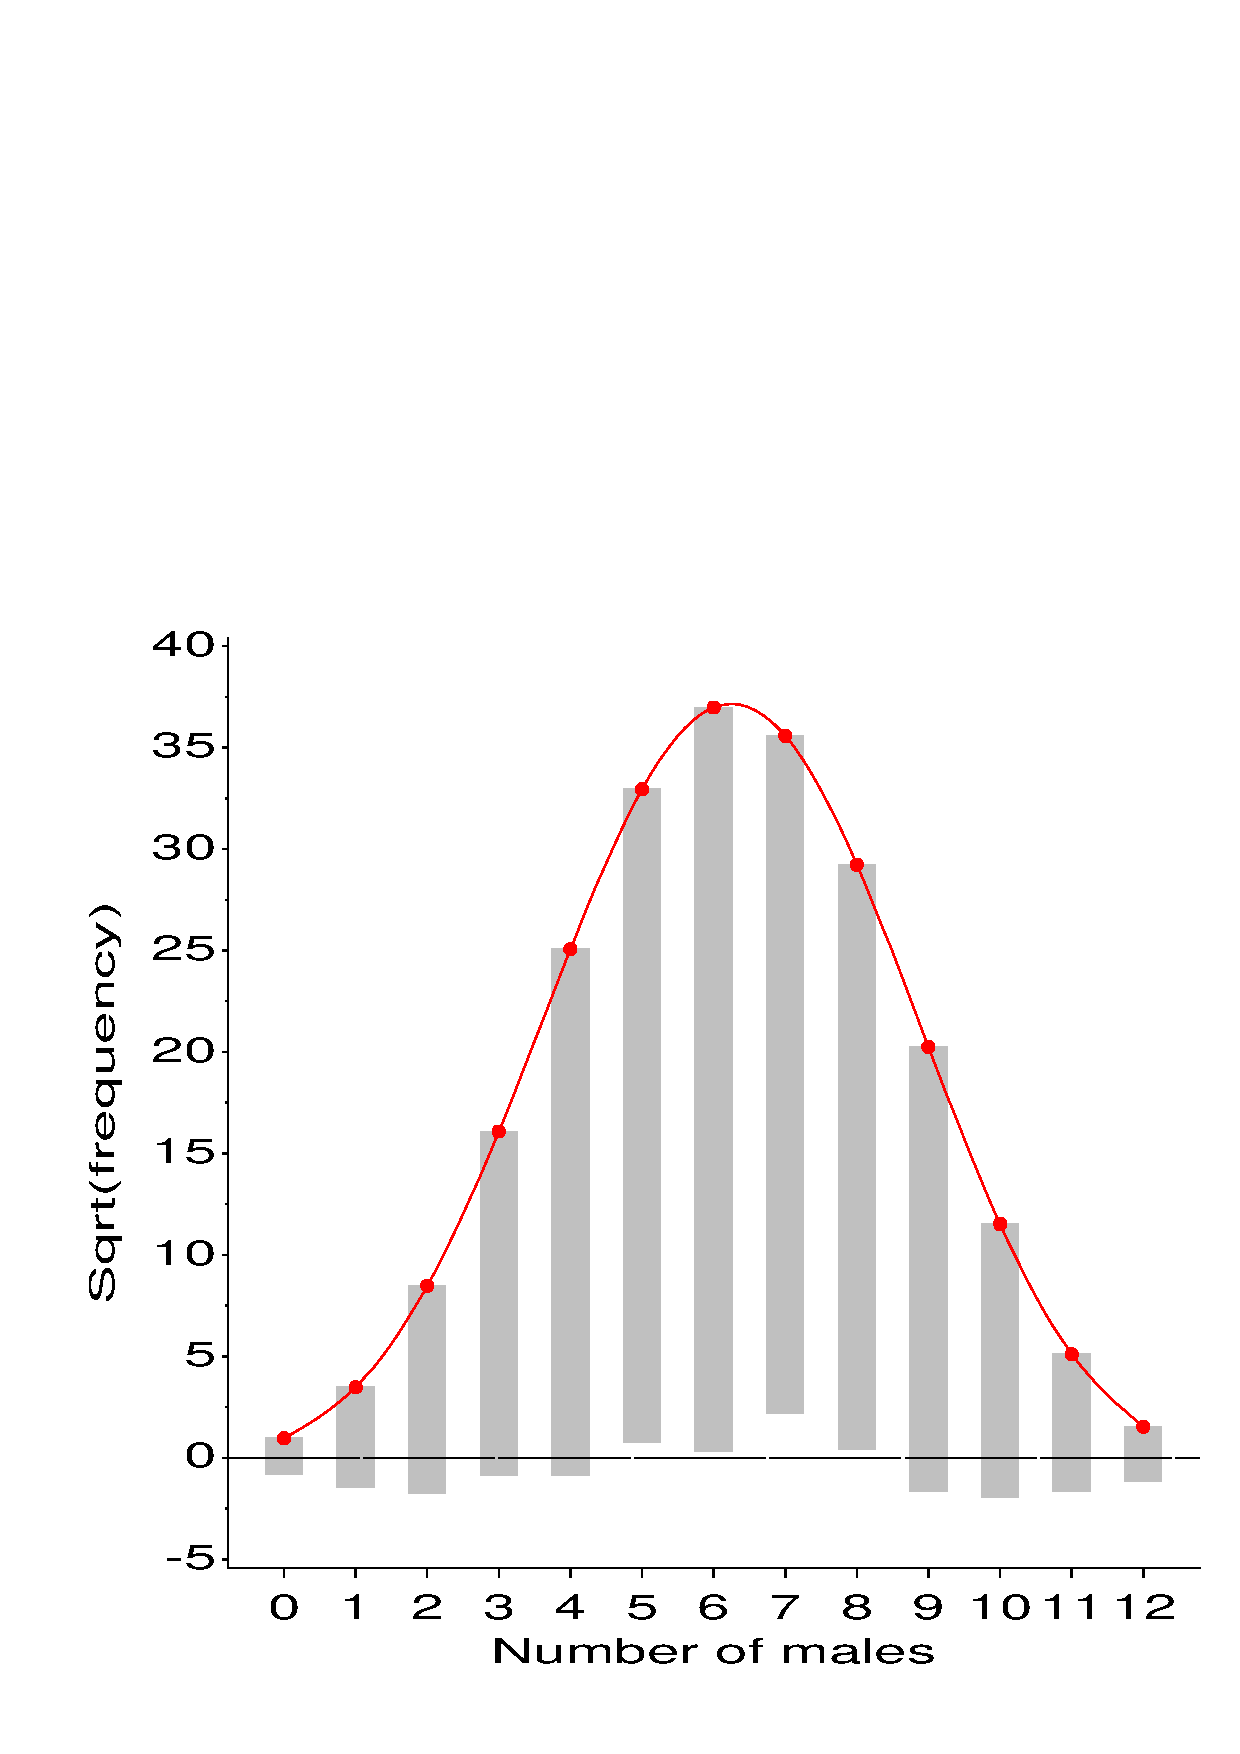
\includegraphics[width=1\linewidth]{saxony}\graphicsfile{ch2/fig/saxony.eps}{}
 \end{minipage}%
 \hfill
 \begin{minipage}[c]{.33\linewidth}
  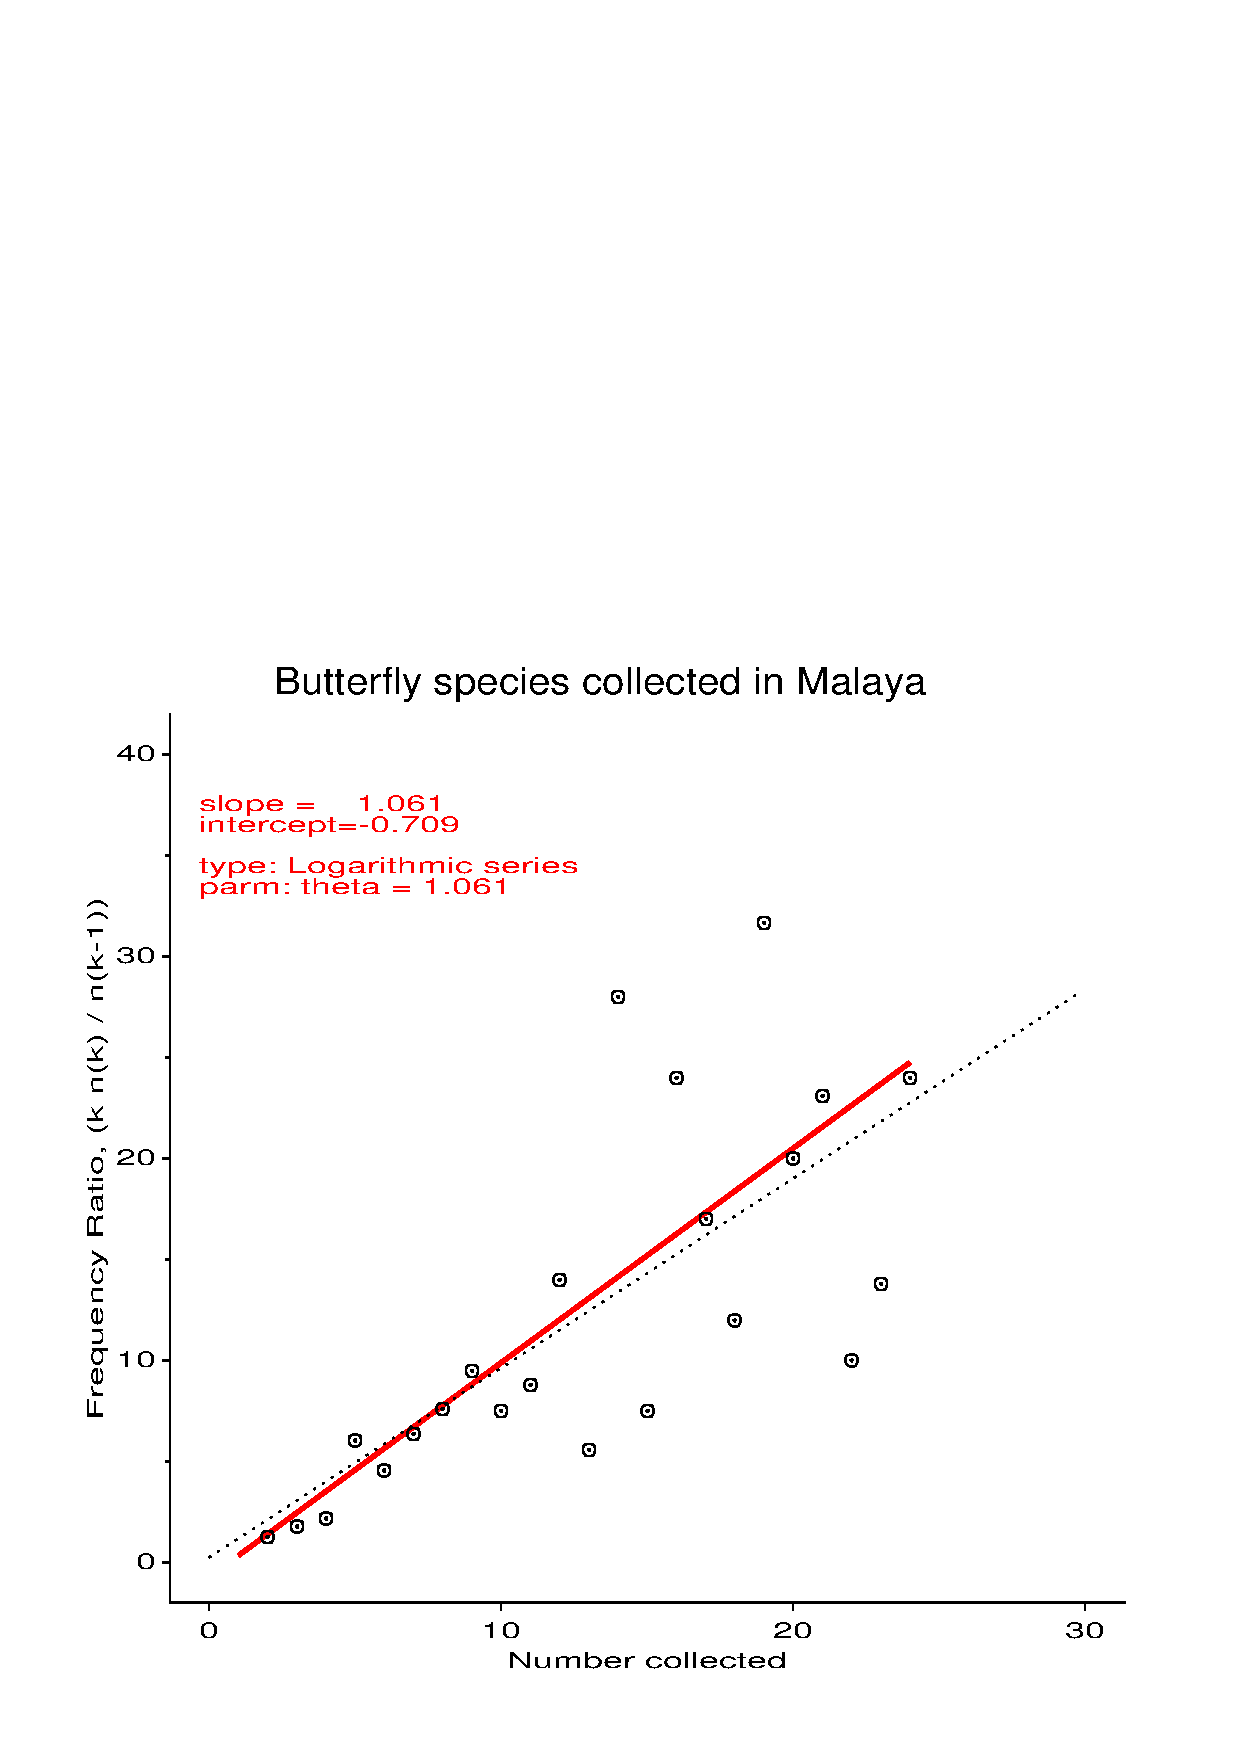
\includegraphics[width=1\linewidth]{orddemo3}\graphicsfile{ch2/fig/orddemo3.eps}{}
 \end{minipage}
 \hfill
 \begin{minipage}[c]{.33\linewidth}
  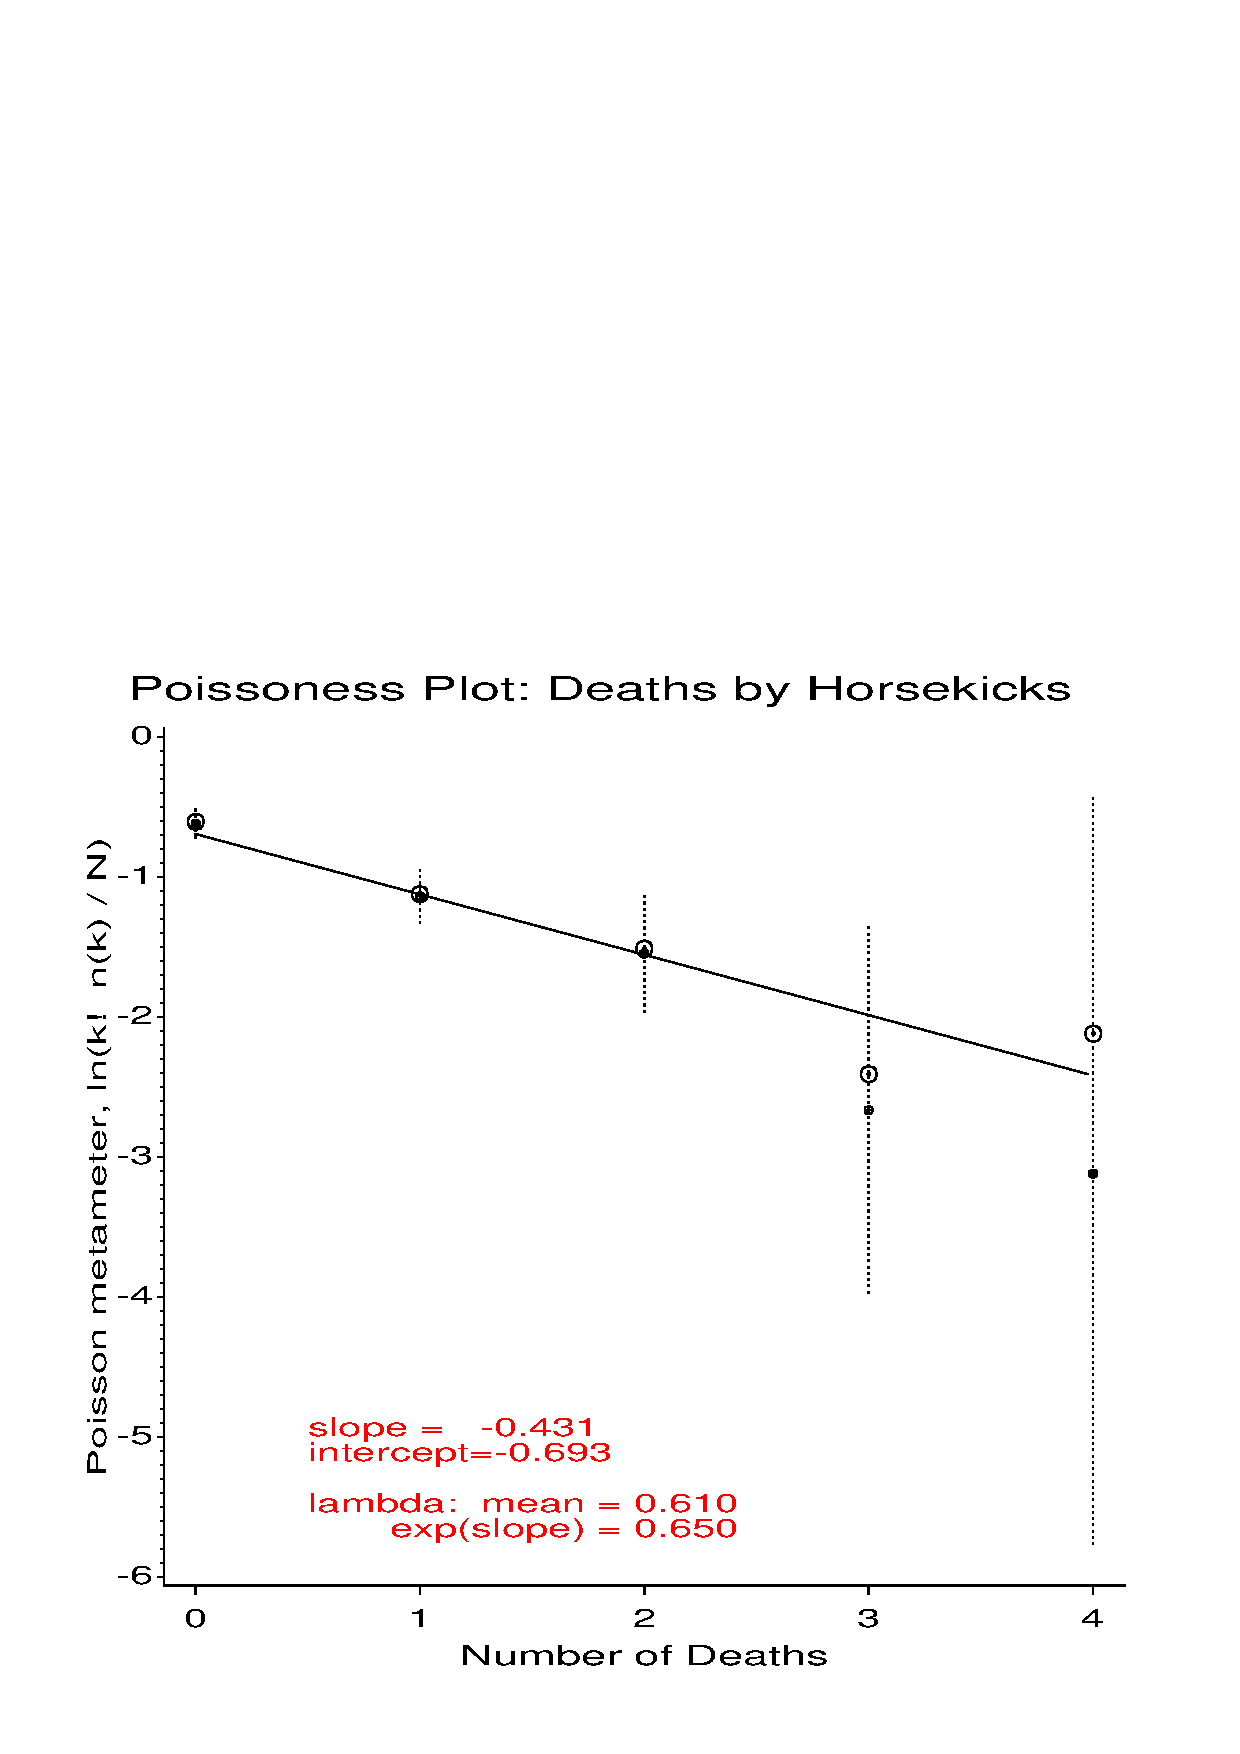
\includegraphics[width=1\linewidth]{poisdemo1}\graphicsfile{ch2/fig/poisdemo1.eps}{}
 \end{minipage}
\end{center}


\begin{quote}
{\Large
Loglinear models are most easily interpreted through
visualizations, including mosaic displays and plots of associated
logit models.  As with logistic regression, diagnostic plots
and influence plots help to assure that the fitted model is
an adequate summary of associations among variables.
}
\end{quote}
\minitoc

\section{Introduction}
\epigraph{We share a philosophy about linear algebra: we think
basis-free, we write basis-free, but when the chips are down we close
the office door and compute with matrices like fury.}
{Irving Kaplansky, in \emph{Paul Halmos: Celebrating 50 Years of Mathematics}}

Loglinear models provide a comprehensive scheme to describe and
understand the associations among two or more categorical variables.
Whereas logit models focus on the prediction of one response factor,
\loglin\ models treat all variables symmetrically, and attempt to
model all important associations among them.  In this sense,
\loglin\ models are analogous to a correlation analysis of continuous
variables, where the goal is to determine the patterns of dependence
and independence among a set of variables.   Nonetheless, when
one variable is indeed a response and the others are explanatory,
certain \loglin\ models are equivalent to logit models for that
response.

\chref{ch:mosaic} and \chref{ch:corresp} introduced some aspects of
\loglin\ models in connection with mosaic displays and correspondence analysis.  
\ix{correspondence analysis}
\ix{mosaic display}
In this chapter, the focus is on fitting and interpreting
\loglin\ models.  The usual analyses, with \PROC{CATMOD} and
\PROC{GENMOD} present the results in terms of tables of parameter
estimates.  Particularly for larger tables, it becomes difficult
to understand the nature of these associations from tables
of parameter estimates.  Instead, we emphasize plots of observed
and predicted probabilities or log odds (when there are one or more response
variables), as well as mosaic and other displays for interpreting a given
model, and residual and influence plots for model diagnostics.
We also illustrate how mosaic displays and \CA\ plot may be used
in a complementary way to the usual numerical summaries, to provide
additional insights into the data.

\secref{sec:loglin-counts} gives a brief overview of \loglin\
models in relation to the more familiar ANOVA and regression models
for quantitative data.
Methods and software for fitting these models are discussed in 
\secref{sec:loglin-fitting}.
When one variable is a response, logit models for that response provide
a simpler, but equivalent means for interpreting and graphing
results of \loglin\ models, as we describe in \secref{sec:loglin-logit}.
Another class of simplified models (\secref{sec:loglin-ordinal})
occurs when one or more of the explanatory variables are ordinal,
and discrete levels might be replaced by numerical values.
\secref{sec:loglin-vietnam} presents an extended example illustrating
the interplay between model fitting and graphical displays.
As in logistic regression models, there are analogs of
model diagnostics for \loglin\ models.
These statistics  and related visualizations are described in
\secref{sec:loglin-infl}.
The final section (\secref{sec:loglin-multiv}) illustrates some
more comprehensive \loglin\ models for two or more response variables.

The models and methods described here attempt to go beyond the typical
presentations of \loglin\ models.   That is, the topics discussed
and examples presented in this chapter
encompass specialized forms of \loglin\ models
for one response variable, for ordinal explanatory variables, and for
multiple response variables.  This treatment is perhaps at the expense of more
basic models, which were examined in \chref{ch:mosaic} and \chref{ch:corresp}
from an exploratory perspective.
The reader may also wish to consult \CDAref{\C 14},
\citet[\C 10]{Allison:99}, and
\citet[\C 4--5]{Zelterman:99} for additional examples of fitting and
interpretation of \loglin\ models using SAS,
and \citet[\C 6--8]{Agresti:90}, or \citet{Christensen:97}
for additional theory and worked examples.


\section{Loglinear models for counts}\label{sec:loglin-counts}

\Loglin\ models have been developed from two formally distinct,
but related perspectives.  The first is a discrete analog of ANOVA models
for quantitative data, where the multiplicative relations among joint and marginal probabilities are transformed into an additive one by transforming
the counts to logarithms.
The second is a discrete analog of regression models, where the log of the
cell frequency is modeled as a linear function of predictors.

For a quantitative response variable, the ANOVA and regression
approaches are melded into a single, \emph{general linear model},
by representing discrete predictors as dummy variables or contrasts.
The ANOVA and regression perspectives provide interchangeable points
of view.  Equivalent models can be fit using \PROC{REG} and
\PROC{GLM}, although each provides different conveniences for
expressing the model in a \pname{MODEL} statement, for model search,
for obtaining separate tests of model terms, diagnostics, and so
forth.

Similarly, for \ctab\ data, \loglin\ models for nominal variables
have a direct relation to ANOVA models, but these models also have
a regression interpretation when discrete classification variables
are represented by dummy variables.  Because the distribution of
counts in a multinomial sample over the cells of the \ctab\ is
Poisson, another generalization of \loglin\ models is to Poisson
regression.  Here,
the log count is modeled as a linear combination
of predictors, but with a Poisson distribution for the errors.

The recognition that the general linear model for quantitative data,
with normally distributed errors, and similar linear models, such as
logistic regression (binomial error distributions), Poisson regression,
and so forth, had similar structure, led to the development of the
\emph{generalized linear model} \citep{McCullaghNelder:89},
of which all are special cases.
Thus, we can fit \loglin\ models using \PROC{CATMOD}, which
follows the ANOVA approach, or with \PROC{GENMOD}, which
follows the GLM approach, and again, each offers somewhat different
conveniences for model expression, testing, and diagnostic output.

\subsection{Loglinear models as discrete ANOVA models}
For two discrete variables, $A$ and $B$, suppose we have a multinomial sample of $n_{ij}$ observations in each cell $i,j$ of an $I \times J$
\ctab.
Let $\pi_{ij}$ be the joint probabilities in the table, and let
$m_{ij} = n_{++} \pi_{ij}$ be the expected cell frequencies under
any model.
Conditional on the observed total count, $n_{++}$,
each count has a Poisson distribution, with mean $m_{ij}$.
Any \loglin\ model may be expressed as a linear model for the $\log m_{ij}$.
For
example, the hypothesis of independence means that the expected
frequencies, \(m_{ij}\), obey
\begin{equation*}%\label{eq:indep}
  m_{ij} = \frac{ m_{i+} \:  m_{+j} } {m_{++}}
  \period
\end{equation*}

This multiplicative model can be transformed to an additive (linear)
model by taking logarithms of both sides:
\begin{equation*}
  \log ( m_{ij} ) = \log ( m_{i+} )  +  \log ( m_{+j} )
 - \log ( m_{++} )
 \comma
\end{equation*}
which is usually expressed in an equivalent form in terms of model
parameters,
\begin{equation} \label{eq:lmain}
\log ( m_{ij} ) = \mu  +  \lambda_i^A +  \lambda_j^B
\end{equation}
where \(\mu\) is a function of the total sample size, \(\lambda_i^A\)
is the ``main effect'' for variable A,
\(\lambda_i^A = \log \pi_{i+} - \overline{\log \pi_{i+}}\),
 and \(\lambda_j^B\) is the
``main effect'' for variable B,
\(\lambda_j^B = \log \pi_{+j} - \overline{\log \pi_{+j}}\).
In model \eqref{eq:lmain}, there
are $1 + I + J$ parameters,  but only $(I-1)+(J-1)$ are separately
estimable, and hence
the same analysis of variance
restrictions are usually applied to the parameters:  \(\sum_i^I \:
\lambda_i^A  = \sum_j^J \:  \lambda_j^B = 0\).  The main effects in
\loglin\ models pertain to differences among the marginal
probabilities of a variable (which are usually not of direct interest).

These sum-to-zero constraints are one way to make  the model \eqref{eq:lmain}
estimable, but other, equivalent restrictions are possible.
Setting the last values, $\lambda_I^A$ and $\lambda_J^B$
to zero (as in \PROC{GENMOD}), defines
$\lambda_i^A = \log \pi_{i+} - \log \pi_{iJ}$, and
$\lambda_j^B = \log \pi_{+j} - \log \pi_{Ij}$,
as deviations from the last, reference category,
but these parameterizations are otherwise identical.
\footnote{The actual parameter values differ under different
parameterizations, but the \emph{difference} between any pair of
parameters, e.g., $\lambda_i^A - \lambda_{i'}^A$,
is the same for all parameterizations.}

Except for differences in notation,
model \eqref{eq:lmain} is formally identical to the ANOVA main-effects model for
a two-factor design:
\begin{equation*}
  E ( y_{ij} ) = \mu  +  \alpha _i  +  \beta _j
\end{equation*}

For a two-way table, a model which \emph{does} allow an association between the variables is the \emph{saturated model},
\begin{equation}\label{eq:lsat}
\log ( m_{ij} ) = \mu  +  \lambda_i^A
+  \lambda_j^B  +  \lambda_{ij}^{AB}
\end{equation}
where again. restrictions must be imposed for estimation:
\begin{equation}\label{eq:lrestrict}
\sum_i^I \,  \lambda_i^A  = 0, \quad
\sum_j^J \,  \lambda_j^B = 0, \quad
\sum_i^I \,  \lambda_{ij}^{AB} =
\sum_j^J \,  \lambda_{ij}^{AB} = 0  \period
\end{equation}
There are thus $I-1$ linearly independent $\lambda_i^A$ row parameters,
$J-1$ linearly independent $\lambda_j^B$ column parameters,
and $(I-1)(J-1)$ linearly independent $\lambda_{ij}^{AB}$ association  parameters.
Again, model \eqref{eq:lsat} is formally similar to the two-factor ANOVA model with interaction:
\begin{equation*}
  E ( y_{ij} ) = \mu  +  \alpha _i  +  \beta _j
  +  ( \alpha  \beta  )_{ij}
\end{equation*}
Hence, associations between variables in \loglin\ models are
analogous to interactions in ANOVA models.  The use of superscripted symbols,
$\lambda_i^A, \lambda_j^B , \lambda_{ij}^{AB}$ rather than separate
Greek letters is a convention in \loglin\ models, and useful mainly
for \mway\ tables.

Models such as \eqref{eq:lmain} and \eqref{eq:lsat} are
examples of \glossterm{hierarchical models}.
This means that the model must contain all lower-order terms contained
within any high-order term in the model.
Thus, the saturated model, \eqref{eq:lsat} contains $\lambda_{ij}^{AB}$,
and therefore must contain $\lambda_i^A $ and $\lambda_j^B$.
As a result, hierarchical models may be identified by the shorthand
notation which lists only the high-order terms: model \eqref{eq:lsat}
is denoted $[A B]$, while model \eqref{eq:lmain} is $[A] [B]$.

\subsection{Loglinear models as discrete GLMs}
In the GLM approach, a \loglin\ model may be cast in the form of a regression
model for $\log m$.
One advantage is that models for tables of any size and structure
may be expressed in a compact form.

For a contingency table of variables $A,B,C,\ldots $, with $N=I\times
J\times K\times \cdots $ cells, let $\vec{n}$ denote a column vector of
the observed counts arranged in standard order, and let $\vec{m}$ denote
a similar vector of the expected frequencies under some model. Then \emph{any}
\loglin\ model may be expressed
in the form
\begin{equation*}
 \log \vec{m} = \mat{X}\vec{\beta}
 \comma
\end{equation*}
where $\mat{X}$ is a known design or model matrix and $\vec{\beta }$ is a
column vector containing the unknown $\lambda $ parameters. For example, for
a $2\times 2$ table, the saturated model \eqref{eq:lsat} with the usual zero-sum constraints \eqref{eq:lrestrict}
can be represented as
\begin{equation*}
\left(
\begin{array}{c}
\log m_{11} \\
\log m_{12} \\
\log m_{21} \\
\log m_{22}
\end{array}
\right) =\left[
\begin{array}{rrrr}
1 & 1 & 1 & 1 \\
1 & 1 & -1 & -1 \\
1 & -1 & 1 & -1 \\
1 & -1 & -1 & 1
\end{array}
\right] \left(
\begin{array}{c}
\mu  \\
\lambda _1^A \\
\lambda _1^B \\
\lambda _{11}^{AB}
\end{array}
\right)
\end{equation*}
Note that only the linearly independent parameters are represented.
$\lambda_2^A = - \lambda_1^A$, because $\lambda_1^A + \lambda_2^A =0$, and
$\lambda_2^B = - \lambda_1^B$, because $\lambda_1^B + \lambda_2^B =0$,
and so forth.

An additional advantage of the GLM formulation is that it makes it easier
to express models with ordinal or quantitative variables.  \PROC{GENMOD}
constructs the model matrix from the terms listed in the \stmt{MODEL}{GENMOD}.
A \pname{CLASS} variable with $K$ levels gives rise to $K-1$ columns
for its main effect and sets of $K-1$ columns in each interaction effect.
\PROC{CATMOD} also constructs the model matrix from the effects listed
on the \stmt{MODEL}{CATMOD} and \stmt{LOGLIN}{CATMOD},
but, quantitative variables are treated nominally in models
specified on the \stmt{LOGLIN}{CATMOD}.
Models which cannot be expressed using the standard syntax may be
represented by entering the model matrix directly.

\subsection{\Loglin\ models for three-way tables}
\Loglin\ models for three-way \ctab s
were described briefly in \secref{sec:mosaic-fitting}.
Each type of model allows associations among different sets of variables
and each has a different independence interpretation, as illustrated in
\tabref{tab:hyp3way}.

For a three-way table, the saturated model, denoted $[ABC]$ is
\begin{equation} \label{eq:lsat3}
  \log \,  m_{ijk}  =
  \mu  +  \lambda_i^A
  +  \lambda_j^B
  +  \lambda_k^C
  +  \lambda_{ij}^{AB}
  +  \lambda_{ik}^{AC}
  +  \lambda_{jk}^{BC}
  +  \lambda_{ijk}^{ABC}
  \period
\end{equation}
This has all variables associated; \eqref{eq:lsat3} fits the data perfectly because
the number of independent parameters equals the number of table cells.
Two-way terms, such as $\lambda_{ij}^{AB}$ pertain to the
partial association between pairs of factors.
The presence of the three-way term, $\lambda_{ijk}^{ABC}$,
means that the partial association (conditional odds ratio) between any pair
varies over the levels of the third variable.

Omitting the three-way term gives the model
$[AB] [AC] [BC]$,
\begin{equation} \label{eq:lno3way}
  \log \,  m_{ijk}  =
  \mu  +  \lambda_i^A
  +  \lambda_j^B
  +  \lambda_k^C
  +  \lambda_{ij}^{AB}
  +  \lambda_{ik}^{AC}
  +  \lambda_{jk}^{BC}
  \comma
\end{equation}
in which all pairs are conditionally dependent. However, for any pair,
the conditional odds ratios are the \emph{same} at all levels of the remaining
variable, so this model is often called the \glossterm{homogeneous association model}.

The interpretation of terms in this model may be illustrated
using the Berkeley admissions data (\exref{ex:berkeley2} and \exref{ex:berkeley3}), for which the factors are Admit,
 Gender, and Department, in a $2 \times 2 \times 6$ table.
In the homogeneous association model,
\begin{equation}\label{eq:berk1}
  \log \,  m_{ijk}  =
  \mu  +  \lambda_i^A
  +  \lambda_j^D
  +  \lambda_k^G
  +  \lambda_{ij}^{AD}
  +  \lambda_{ik}^{AG}
  +  \lambda_{jk}^{DG}
  \comma
\end{equation}
the $\lambda$-parameters have the following interpretations:
\begin{itemize}
\item The main effects, $\lambda_i^A , \lambda_j^D$ and $\lambda_k^G$
   pertain to differences in the one-way marginal probabilities.
    Thus $\lambda_j^D$ relates to differences in the total number of applicants
    to these departments, while $\lambda_k^G$ relates to the differences
    in the overall numbers of men and women applicants.
\item $\lambda_{ij}^{AD}$ describes the partial association between
   admission and department, that is  different admission rates across
   departments (controlling for gender).
\item $\lambda_{ik}^{AG}$ relates to the association between
   admission and gender, controlling for department.
    This term, if significant, might be interpreted as indicating
   gender-bias in admissions.
\item $\lambda_{jk}^{DG}$, the association between
 department and gender, indicates whether males and females apply
 differentially across departments.
\end{itemize}

\section{Fitting discrete distributions}\label{sec:discrete-fit}

Often interest is focused on how closely such data follow a
particular distribution, such as the Poisson, binomial, or geometric
distribution.  Usually this is examined with a classical (Pearson)
goodness-of-fit chi-square test,
\glosstex{chi-square test}

\begin{equation}\label{eq:chi2}
  \chi^2 = \sum_{k=1}^K \:
  \frac{{ ( n_k - N \hat{p}_k ) }^2}
  { N \hat{p}_k }  \sim \chi^2_{( K-s-1 )}
  \comma
\end{equation}
where there are $K$ frequency classes, 
$s$ parameters have been estimated from the data and
\(\hat{p}_k\) is the estimated probability of each basic count,
under the null hypothesis that the data follows the chosen distribution.
An alternative test statistic is the likelihood-ratio $G^2$
statistic,
\begin{equation}\label{eq:g2}
 G^2 = \sum_{k=1}^K \: n_k \log ( n_k / N \hat{p}_k )
 \comma
\end{equation}
when the $\hat{p}_k$ are estimated by maximum likelihood,
which also has an asymptotic $\chi^2_{(K - s - 1)}$ distribution.
``Asymptotic'' means that these are large sample tests.
A common rule of thumb is that all expected frequencies
should exceed one and that fewer than 20\% should be less than 5.

For the horse kick data, the mean is 122/200 = .610, and calculation
of Poisson probabilities (\texttt{PHAT}), expected frequencies, and
contributions to \(\chi^2\) \eqref{eq:chi2} are shown below.
\ixd{deaths by horsekick}

\begin{center}
\begin{alltt}
 k     nk      p        phat         exp     chisq

 0    109    0.545    0.54335    108.670    0.00100
 1     65    0.325    0.33144     66.289    0.02506
 2     22    0.110    0.10109     20.218    0.15705
 3      3    0.015    0.02056      4.111    0.30025
 4      1    0.005    0.00313      0.627    0.22201
      ===                        =======    =======
      200                        199.915    0.70537 \(\sim \chi\sp2 (3)\)
\end{alltt}
\end{center}

In this case the \(\chi^2\) shows an exceptionally good (perhaps unreasonably
good?) fit.  In the word frequency example
(\exref{ex:madison1}), the fit of the Poisson
turns out not to be close at all.  However, even a close fit may show
something interesting, if we know how to look; conversely, it is
useful to know why or where the data differ from a chosen model.

\subsection{The \macro{GOODFIT}}
The \macro{GOODFIT} (see \macref{mac:goodfit}) carries out Pearson \chisq{} and \LR{} goodness-of fit tests
for the uniform, binomial, Poisson, negative binomial,
 logarithmic series, and geometric distributions,
as well as any discrete (multinomial) distribution whose probabilities you can specify.
The data may consist either of individual observations on a single
variable, or a grouped frequency distribution in the form
shown in \tabref{tab:horskick}.
The parameter(s) of the distribution may be specified as constants
or may be estimated from the data.

\begin{comment}  %%% begin stuff deleted
The macro is used as follows%
\footnote{In subsequent descriptions of macros in the text
we simply give references to the documentation provided in Appendix \ref{ch:macros} and provide examples of usage.}%
:
\aunote{Should we take this out?}
\begin{listing}
\%goodfit(data=\emph{SASdatasetname},
   var=\emph{variablename},
   freq=\emph{variablename},
   dist=\emph{distribution},
   parm=\emph{parameters},
   sumat=\emph{value},
   format=\emph{SASformat},
   out=\emph{outputdatasetname},
   outstat=\emph{statisticsdatasetname});
\end{listing}
\end{comment}  
The macro parameters are described in \macref{mac:goodfit}.
We illustrate its use in \exref{ex:weldon} and \exref{ex:federalist} below.

\begin{Example}[weldon]{Weldon's dice}
The data from \tabref{tab:dice}
can be fit to a binomial distribution as shown below.
Note that, because the frequencies have been lumped for 10--12
successes, it is necessary to
\begin{seriate}
\item Input frequencies for all values of $k = 0, \dots, 12$,
using missing values for the frequencies beyond $k=10$;
\item specify \texttt{sumat=10} in the macro call.
\end{seriate}
%% table from data set dice (dice.sas) generated 26DEC97
\begin{table}[htb]
\caption{Frequencies of a 5 or 6 in throws of 12 dice}
\label{tab:dice}
 \begin{center}
  \begin{tabular}{rr}
  \hline
Number of  & Frequency \\
5s or 6s ($k$) & ($n_k$) \\
  \hline
0 & 185 \\
1 & 1149 \\
2 & 3265 \\
3 & 5475 \\
4 & 6114 \\
5 & 5194 \\
6 & 3067 \\
7 & 1331 \\
8 & 403 \\
9 & 105 \\
10+ & 18 \\
    & N=26306 \\
  \hline
  \end{tabular}
 \end{center}
\end{table}


The first call to the \macro{GOODFIT} fits the binomial distribution
with parameter $p = \frac13$, assuming the dice to be fair,
and produces the output shown in \outref{out:dice.1} and \outref{out:dice.2}.
The \chisq{} statistics indicate that the fit is poor,
and the pattern of residuals
suggests that $p > \frac13$
(the observed frequencies for larger values of $k$ are all
greater than the expected frequencies).
\begin{Output}
\caption{Fitting Binomial(12,$\frac13$) to Weldon's dice data: Observed and fitted frequencies}\label{out:dice.1}
\verbatiminput{ch2/out/dice.1}
\end{Output}
\begin{Output}
\caption{Fitting Binomial(12,$\frac13$) to Weldon's dice data: Goodness of fit tests}\label{out:dice.2}
\verbatiminput{ch2/out/dice.2}
\end{Output}

The second call to the \macro{GOODFIT} allows the
 parameter $p$ to be estimated from the data, giving $\hat{p} = .3377$,
and produces the output shown in \outref{out:dice.3} and \outref{out:dice.4}.
The fit is much better---in fact, quite satisfactory.
So, Weldon's dice differed minutely from being absolutely fair,
but with over 26,000 tosses it is easy to detect the difference.
\begin{Output}
\caption{Fitting Binomial(12,$p$) to Weldon's dice data: Observed and fitted frequencies}\label{out:dice.3}
\verbatiminput{ch2/out/dice.3}
\end{Output}
\begin{Output}
\caption{Fitting Binomial(12,$p$) to Weldon's dice data: Goodness of fit tests}\label{out:dice.4}
\verbatiminput{ch2/out/dice.4}
\end{Output}
\end{Example}

\begin{Example}[federalist]{Federalist papers}
The data on the occurrences of the word \emph{may} in Madison's
Federalist Papers (\tabref{tab:madison})
are fit to both the Poisson and Negative binomial distributions as shown below.  In each case, the parameters are estimated from the data.  The output for the Poisson distribution appears
in \outref{out:madfit.1} and \outref{out:madfit.2}.
The results for the Negative binomial distribution appear
in \outref{out:madfit.3} and \outref{out:madfit.4}.
\begin{listing}
%include catdata(madison);
%goodfit(data=madison, var=count, freq=blocks, dist=poisson);

%goodfit(data=madison, var=count, freq=blocks, dist=negbin);
\end{listing}

\begin{Output}
\caption{Fitting the Poisson($\lambda$) to the Federalist Papers data: Observed and fitted frequencies}\label{out:madfit.1}
\small
\verbatiminput{ch2/out/madfit.1}
\end{Output}
\begin{Output}
\caption{Fitting the Poisson($\lambda$) to the Federalist Papers data: Goodness of fit tests}\label{out:madfit.2}
\verbatiminput{ch2/out/madfit.2}
\end{Output}

\begin{Output}
\caption{Fitting the Negative binomial($n, p$) to the Federalist Papers data: Observed and fitted frequencies}\label{out:madfit.3}
\small
\verbatiminput{ch2/out/madfit.3}
\end{Output}
\begin{Output}
\caption{Fitting the Negative binomial($n, p$) to the Federalist Papers data: Goodness of fit tests}\label{out:madfit.4}
\small
\verbatiminput{ch2/out/madfit.4}
\end{Output}
\end{Example}

\subsection{Plots of observed and fitted frequencies}
Plots of the observed and fitted frequencies can help to show
both the shape of the theoretical distribution we have fitted and the
pattern of any deviations between our data and theory.

\figref{fig:madfit1} shows the fit of the Poisson distribution to the Federalist papers data, using one common form of plot that is sometimes
used for this purpose.
In this plot, observed frequencies are shown by bars and fitted
frequencies are shown by points, connected by a smooth (spline)
curve.%
%\footnote{Using a curve has the unfortunate }

Such a plot, however, is dominated by the largest frequencies,
making it hard to assess the deviations among the smaller frequencies.
To make the smaller frequencies more visible, \citet{Tukey:77}
suggest plotting the frequencies  on a square-root scale,
which he calls a \emph{rootogram} (see \figref{fig:madfit2}).
An additional improvement is to move the rootogram bars so their tops
are at the expected frequencies (giving a \emph{hanging rootogram}, \figref{fig:madfit3}).
This has the advantage that we can more easily judge the pattern
of departures against the horizontal reference line at 0, than
against the curve.
A final variation is to emphasize the differences between the
observed and fitted frequencies by drawing the bars to show the
gaps between the 0 line and the (observed-expected) difference
(\figref{fig:madfit4}).

These plots are produced by the \macro{ROOTGRAM} using the (default)
\texttt{OUT=FIT}
\Dset\ from the \macro{GOODFIT}:
%% input: /users/faculty/friendly/sasuser/catdata/madfit.sas
%% last modified: 08-Apr-99  8:31
\begin{listing}
title "Instances of 'may' in Federalist papers" ;
%include catdata(madison);
%goodfit(data=madison, var=count, freq=blocks, dist=poisson, out=fit);

title;
%rootgram(data=fit, var=count, obs=blocks, btype=0, func=none);  /* a */
%rootgram(data=fit, var=count, obs=blocks, btype=0);             /* b */
%rootgram(data=fit, var=count, obs=blocks);                      /* c */
%rootgram(data=fit, var=count, obs=blocks, btype=dev);           /* d */
\end{listing}


% subfigmatrix 2 x 2
\begin{figure}[htb]
 \begin{subfigmatrix}{2}
 \subfigure[Histogram]{\label{fig:madfit1}%
  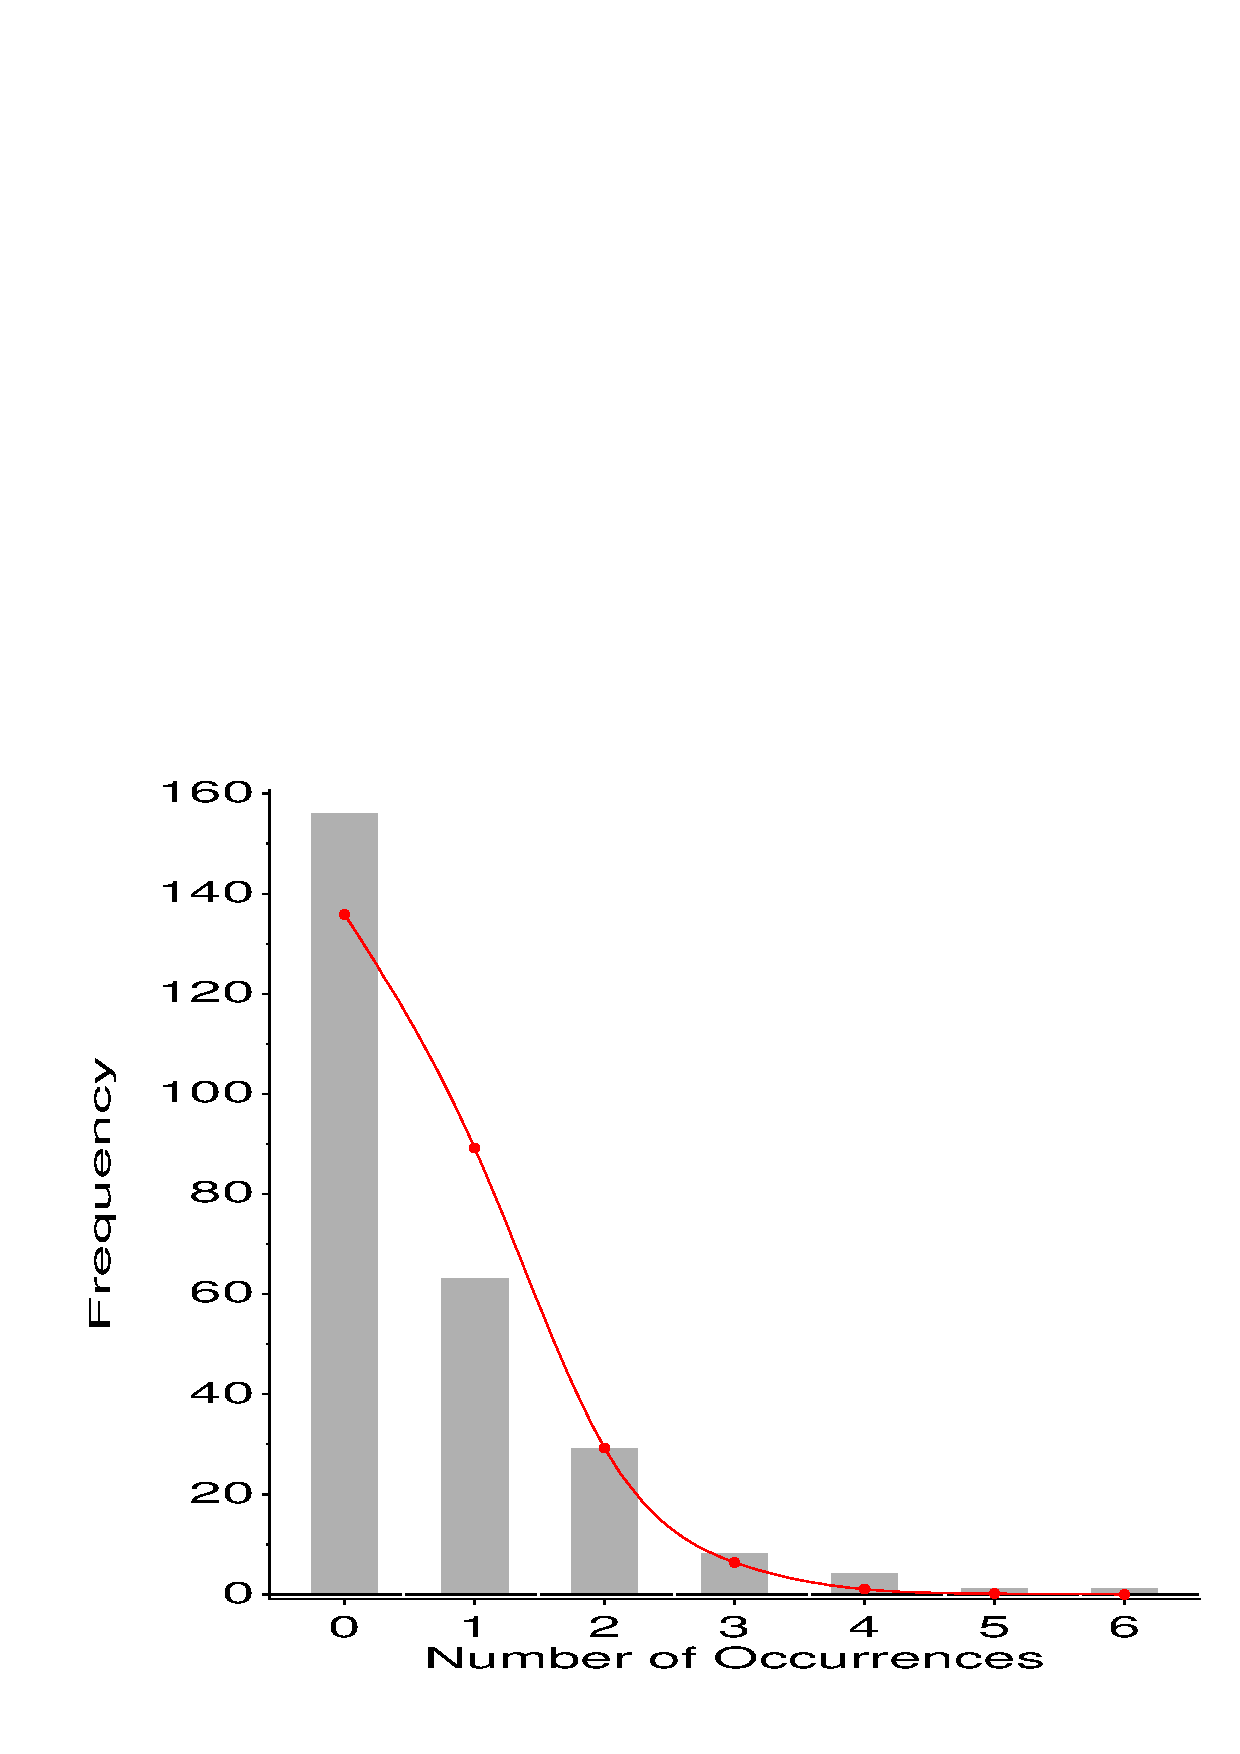
\includegraphics{madfit1}\graphicsfile{ch2/fig/madfit1.eps}{}
 }
 \subfigure[Rootogram]{\label{fig:madfit2}%
  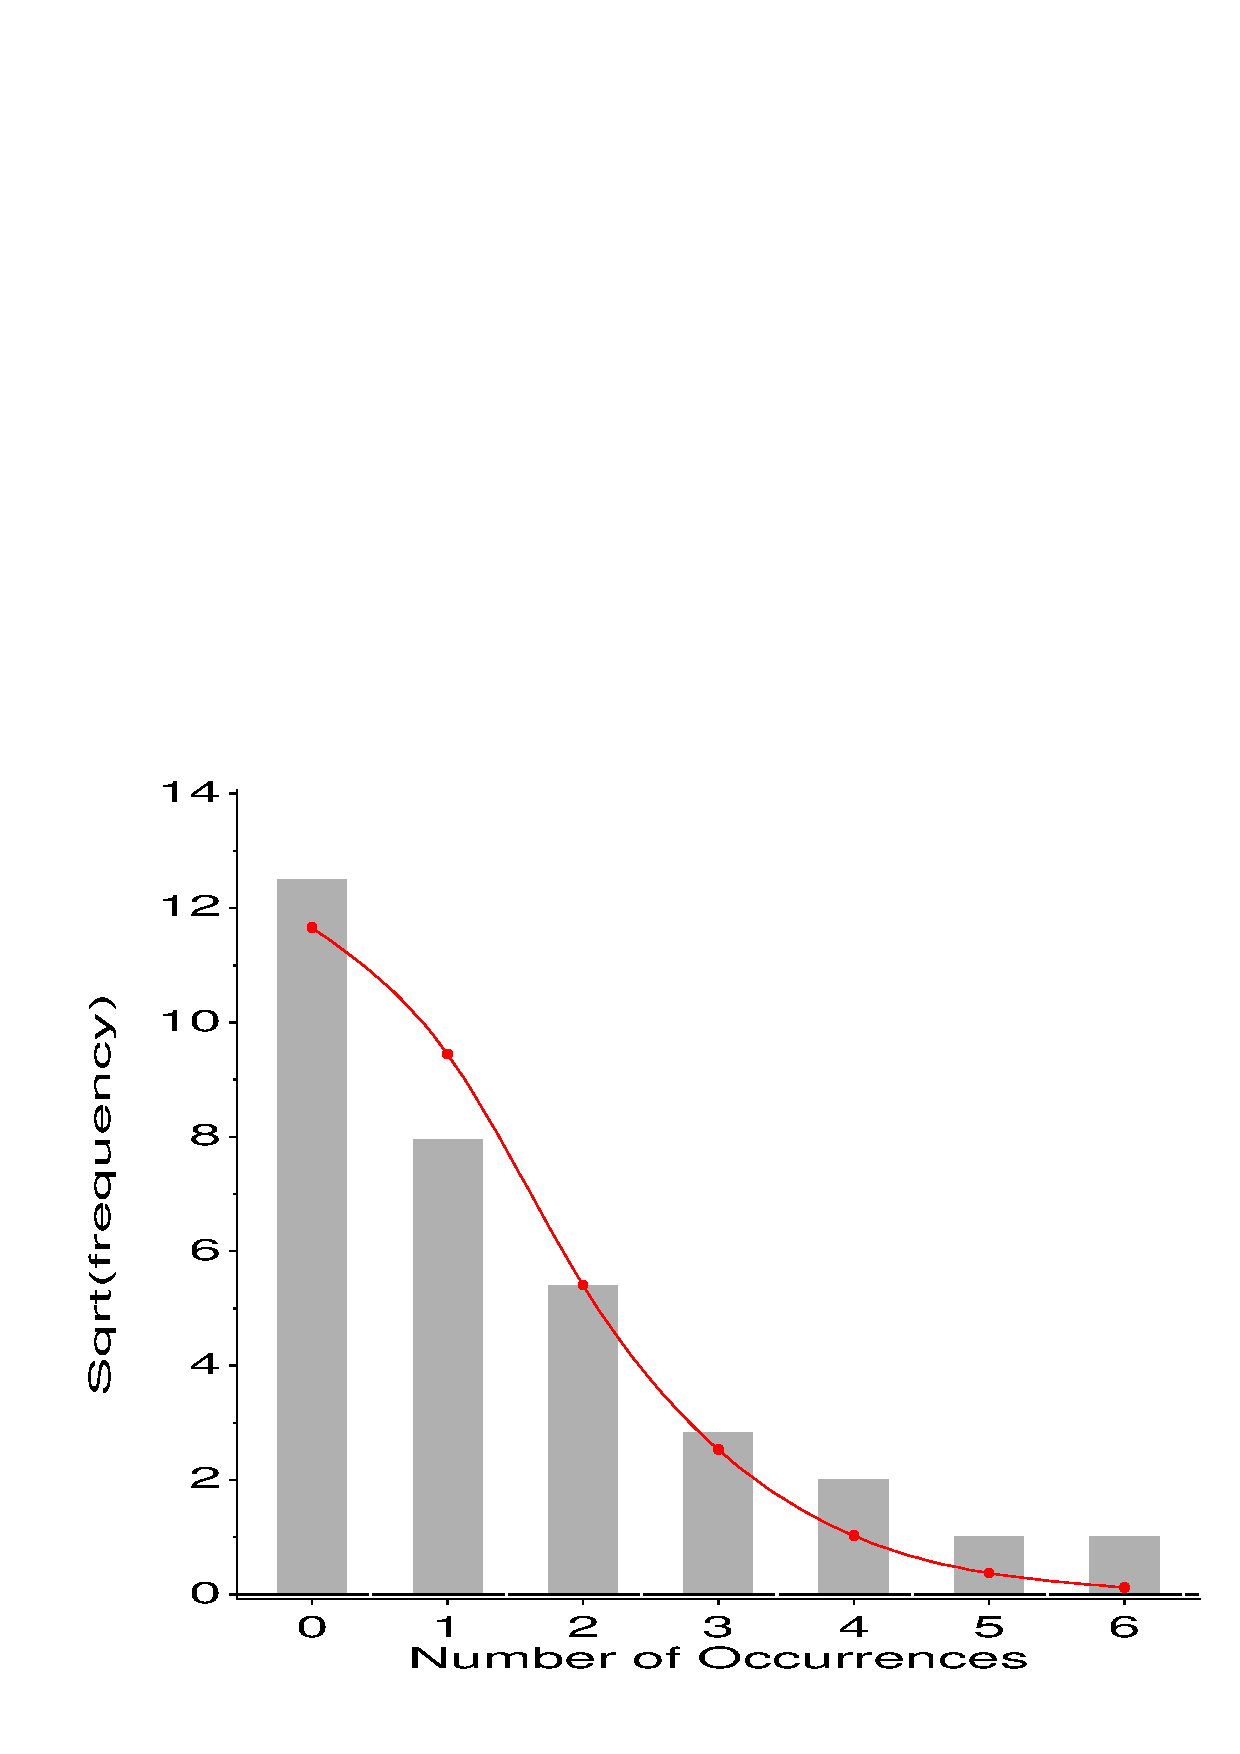
\includegraphics{madfit2}\graphicsfile{ch2/fig/madfit2.eps}{}
 }
 \subfigure[Hanging rootogram]{\label{fig:madfit3}%
  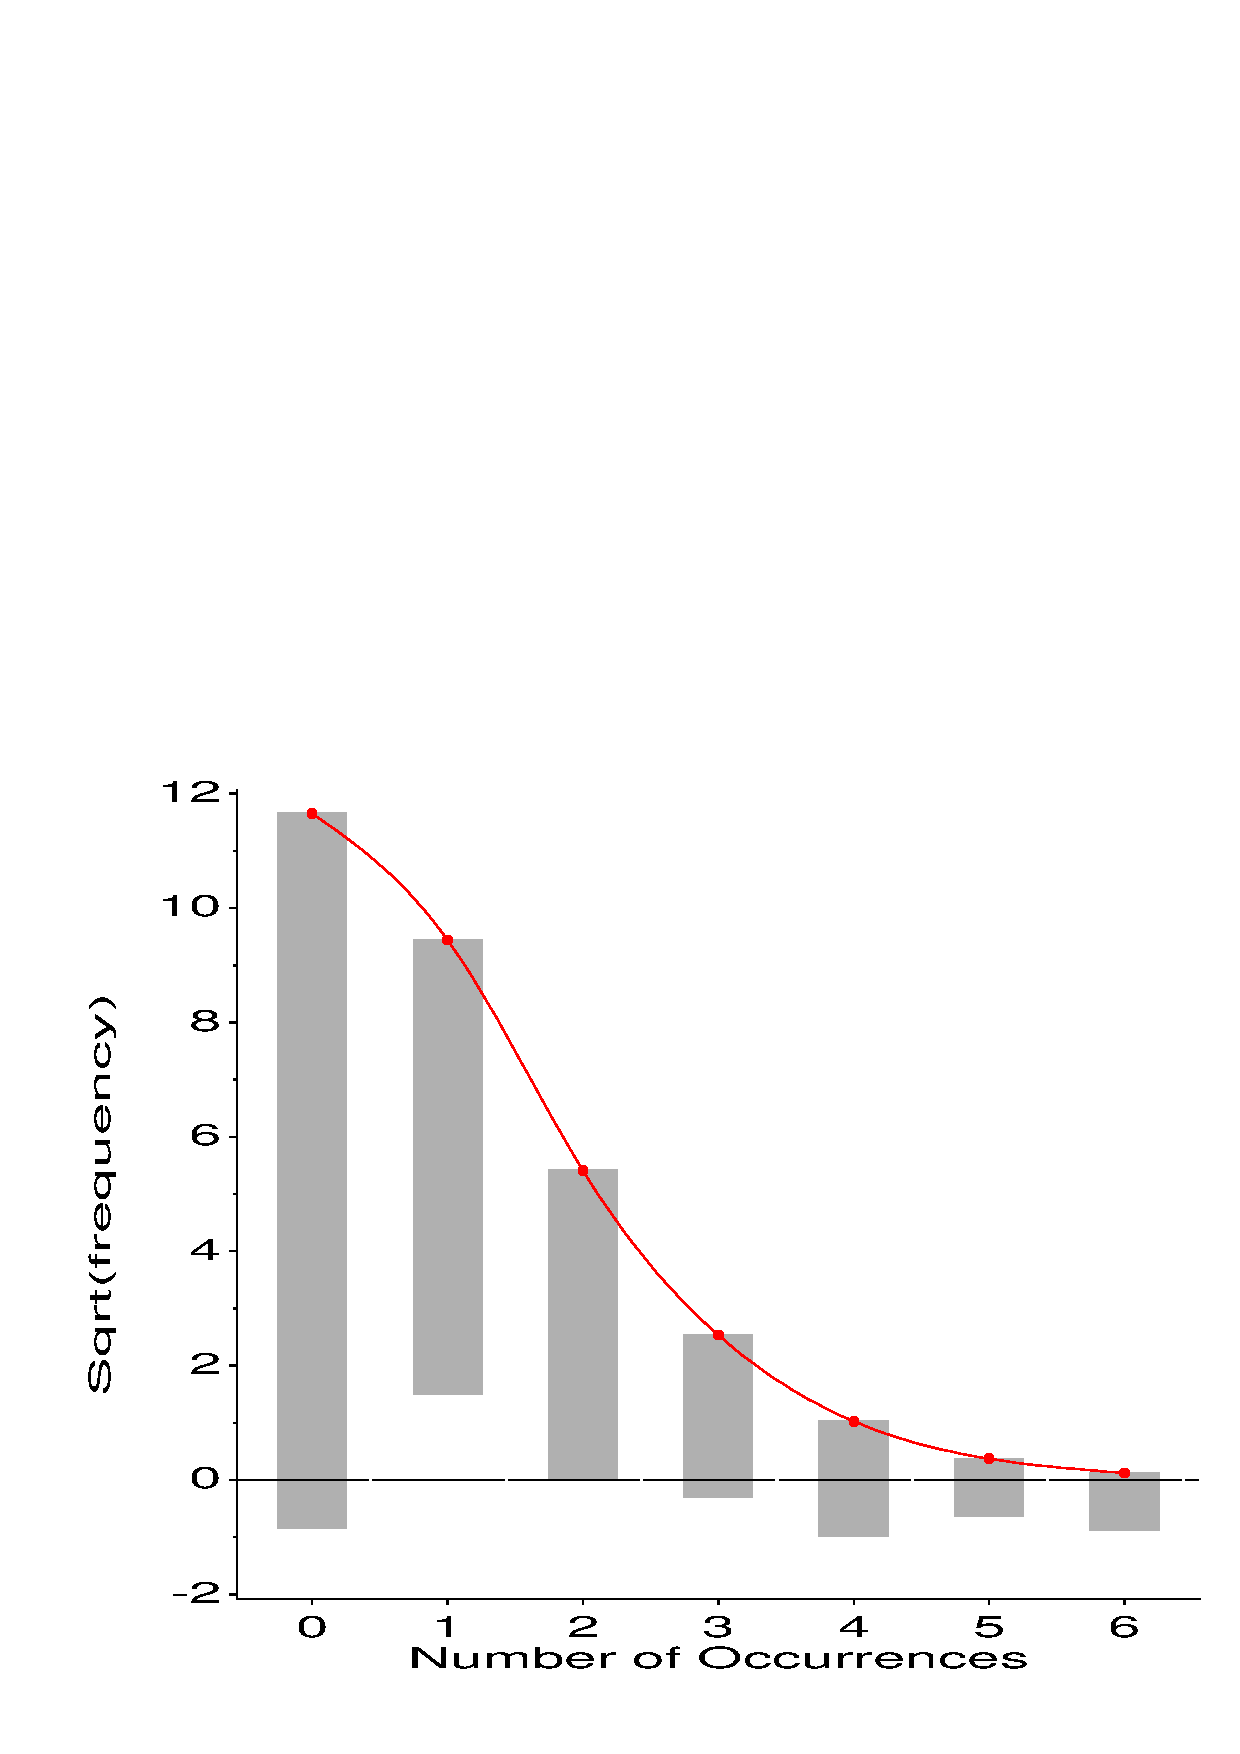
\includegraphics{madfit3}\graphicsfile{ch2/fig/madfit3.eps}{}
 }
 \subfigure[Deviation rootogram]{\label{fig:madfit4}%
  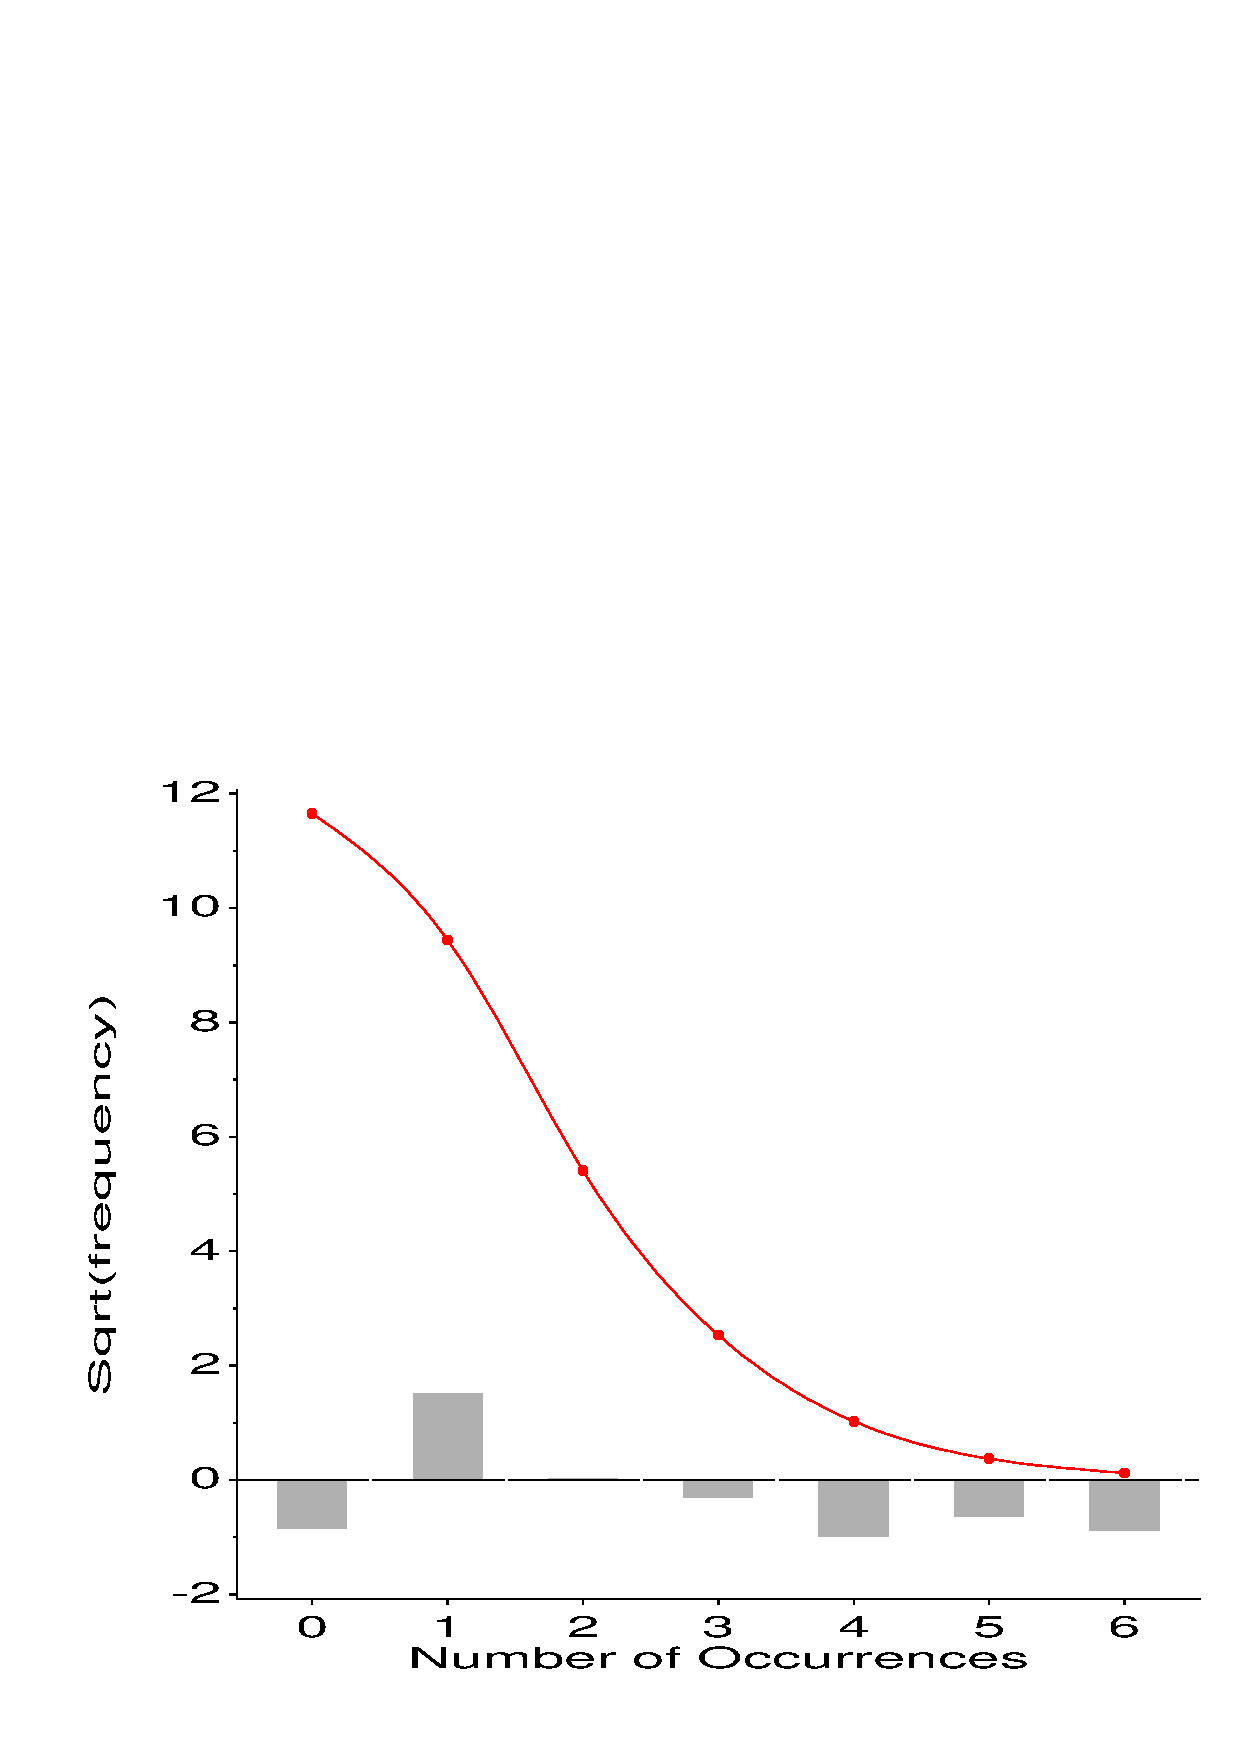
\includegraphics{madfit4}\graphicsfile{ch2/fig/madfit4.eps}{}
 }
 \end{subfigmatrix}
 \caption[Plots of observed and fitted frequencies]{Plots of observed and fitted frequencies
 for the Federalist Papers data, Poisson model.  Each panel shows the fitted frequencies as a smooth
 curve and observed frequencies as a bar.  Panel (a) raw frequencies;
 panels (b)-(d) on a square-root scale, to emphasize smaller frequencies.  Panel (c) is a hanging rootogram, where observed - fitted differences can be judged relative to the horizontal line. Panel (d) shows only the difference between the observed and fi

tted frequency.}\label{fig:madfit}
\end{figure}


\subsection{The \macro{ROOTGRAM}}\label{discrete-root}
The \macro{ROOTGRAM} (\macref{mac:rootgram}) displays observed and fitted frequencies
for a \Dset\ in any of the forms shown in \figref{fig:madfit}.
The input \Dset\ is usually of the form of the output
\texttt{OUT=} \Dset\ produced by the \macro{GOODFIT}.

\begin{Example}[federalist2]{Federalist papers}
We have seen that the negative binomial produces a better fit to the
Federalist Papers data.  The hanging rootogram (\figref{fig:madfit5}),
produced by the statements below, is characteristic of a decent fit.
\begin{listing}
%include catdata(madison);
%goodfit(data=madison, var=count, freq=blocks, dist=negbin, out=fit2);
%rootgram(data=fit2, var=count, obs=blocks, btype=dev);
\end{listing}
%\begin{figure}
%\fig{madfit5.eps}{scale=.7}{madfit5}{Hanging rootogram for the Federalist Papers data, Negative binomial model}
\fig{madfit5}{scale=.7}{Hanging rootogram for the Federalist Papers data, Negative binomial model}
%\end{figure}
\end{Example}


\begin{Example}[saxony1]{Families in Saxony}
Geissler
(cited in \citet{SokalRholf:69}
and \citet{Lindsey:95})
tabulated a huge \Dset\ on sex distributions in families in Saxony
in the 19th century.  Included were $N=6115$ families with $n=12$ children,
which might reasonably be expected to follow a Bin(12,$p$) distribution.
The data are input and fit as shown below.
%% input: /users/faculty/friendly/sasuser/catdata/saxony.sas
%% last modified: 08-Jan-98  9:29
\begin{listing}
title 'Number of males in 6115 families in Saxony';
data saxony;
   do males = 0 to 12;
      input families @;
      output;
      end;
   label males='Number of males'
      families='Number of families';
datalines;
3  24  104  286  670  1033  1343 1112  829  478  181  45  7
;

%goodfit(data=saxony, var=males, freq=families, dist=binomial);

title;
%rootgram(data=fit, var=males, obs=families, exp=exp);
\end{listing}


The fitted distribution, using the estimated proportion of males,
$p = .5192$ is shown in \outref{out:saxony.1};
the goodness of fit tests shown in \outref{out:saxony.2}
indicate that the fit of the Binomial is not good.
The hanging rootogram in \figref{fig:saxony} shows why---%
there is a systematic pattern of deviations from the Binomial,
which produces fitted frequencies too high in the middle and too small
in the tails.
The lack of fit might be ascribed to violations of the assumptions---%
a constant probability of a male birth over a long time span
is a good possibility.
\footnote{\citet[p. 131]{Lindsey:95}
fits a double binomial model with one extra parameter,
and achieves a much better fit, but this too
shows significant lack of fit, not surprising considering the
enormous sample size.}
\begin{Output}
\caption{Fit of the Binomial($12, p$) to the Families in Saxony data: Observed and fitted frequencies}\label{out:saxony.1}
\small
\verbatiminput{ch2/out/saxony.1}
\end{Output}
\begin{Output}
\caption{Fit of the Binomial($12, p$) to the Families in Saxiony data: Goodness of fit tests}\label{out:saxony.2}
\small
\verbatiminput{ch2/out/saxony.2}
\end{Output}

\begin{figure}[htb]
  \centering
  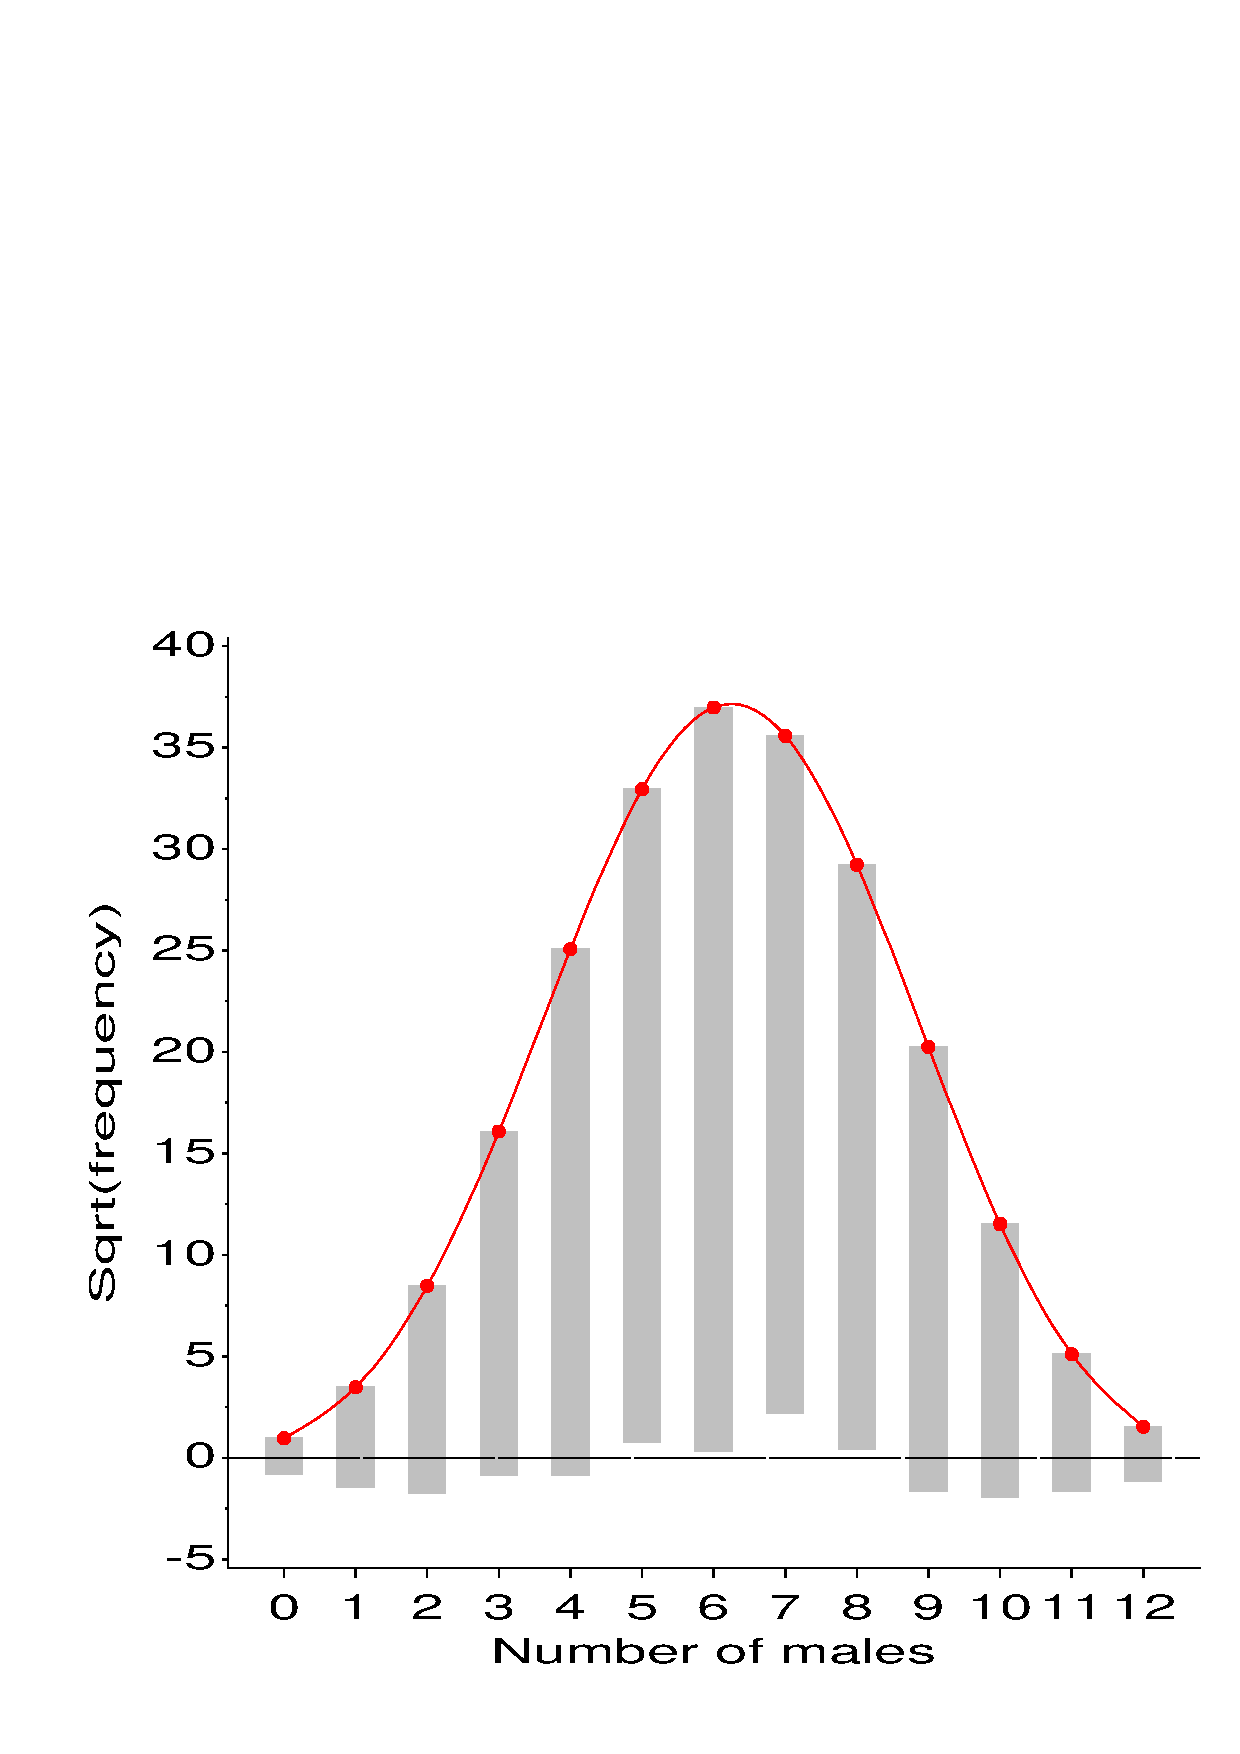
\includegraphics[scale=.5]{saxony}\graphicsfile{ch2/fig/saxony.eps}{}
  \caption[Hanging rootogram for Saxony families, Binomial model]{Hanging rootogram for Saxony families, Binomial($12, p$) model.
The systematic pattern of deviations shows that the Binomial model is not completely adequate for these data.}\label{fig:saxony}
\end{figure}
\end{Example}


\subsection{Maximum likelihood estimation}
\secref{sec:discrete-distrib} described the common discrete distributions,
their probability functions, and sample estimates.
Here we consider the general case.
Suppose we have a multinomial sample of
$K$ ``groups'', with frequencies of $n_k$ in group
$k$, and $\sum_k n_k = N$.
Suppose further that we have a probability model which specifies
the probability, \( \pi_k (\vec{\theta}), \: k = 1, 2, \dots ,  K \),
of an observation in group $k$, where $\vec{\theta}$ is a vector
of $s \geq 0$ parameters of the distribution
and $\sum_k \pi_k (\vec{\theta}) = 1$.

The likelihood, $\mathcal{L}$, is the probability of the data as
a function of the parameters,

\begin{equation*}
  \mathcal{L}(\vec{\theta}) = n ! \prod_{k=1}^K \frac{\pi_k (\vec{\theta})^{n_k}}{n_k !}
\end{equation*}

We can determine the value(s) of $\vec{\theta}$ which maximize $\mathcal{L}$
by maximizing the log-likelihood,

\begin{equation}\label{eq:loglikelihood}
 \ell(\vec{\theta}) \equiv
 \log \mathcal{L}(\vec{\theta}) = \log n ! +
  \sum_{k=1}^K n_k \log \pi_k (\vec{\theta}) - \sum_{k=1}^K \log n_k !
\end{equation}
The maximum likelihood estimate (MLE) of $\vec{\theta}$ will be
the value $\hat{\vec{\theta}}$ which is the solution of the
estimating equations
\begin{equation*}
\frac{\partial \log \mathcal{L}(\vec{\theta})}{\partial \vec{\theta}_i} = 0
\quad\quad i=1, 2, \dots s
\end{equation*}

For example, for the geometric distribution with probability
function \eqref{eq:geomf}, the log-likelihood is
\begin{equation*}
 \ell(\vec{\theta})   = n \log \theta +
  \sum_{k=1}^K (n_k - 1) \log (1-\theta)
\end{equation*}
which gives the estimating equation,
\begin{equation*}
\frac{\partial \ell(\theta)}{\partial \theta} =
\frac{(\sum_k n_k) - n}{1-\theta} + \frac{n}{\theta} = 0
\end{equation*}
whose solution is $\hat{\theta} = 1/\bar{k}$.  The fitted probabilities
under the geometric model
are then $\pi_k (\hat{\theta}) = (1 - \hat{\theta})^{k-1} \hat{\theta}$.

Having found the maximum likelihood estimate of the parameters, the
likelihood ratio
goodness-of-fit \GSQ{} statistic compares the maximized value of the
log-likelihood to the maximized log-likelihood of an unrestricted model
where the probabilities are only constrained so that $\sum_k \pi_k =1$.
In this case, there are $s=0$ parameters, and we symbolize the log-likelihood
by $ \ell(\theta_0) \equiv \ell(\vec{\pi})$.  For a multinomial sample this is

\begin{equation}\label{eq:loglikelihood0}
 \ell(\vec{\theta}_0)  = \log n ! +
  \sum_{k=1}^K n_k \log \pi_k  - \sum_{k=1}^K \log n_k !
\end{equation}
Maximizing \eqref{eq:loglikelihood0} subject to $\sum_k \pi_k =1$
gives $\hat{\pi}_k = n_k / N$.
The likelihood ratio statistic is

\begin{equation}\label{eq:likeratio}
 G^2 = -2 \log \left[
 \frac{\mathcal{L}(\vec{\theta}_0)}{\mathcal{L}(\vec{\theta})}
 \right]
 = 2 [ \ell(\vec{\theta}) - \ell(\vec{\theta}_0) ]
 = 2 \sum_{k=1}^{K} n_k \log \left( \frac{n_k}{N \pi_k (\hat{\theta}) } \right)
\end{equation}
which follows an asymptotic chi-square distribution with $K-1-s$ degrees
of freedom.


\subsection{Fitting discrete distributions as \loglin\ models}
In \secref{sec:pwrseries}, I described how the common discrete distributions
are all members of the general power series family.
Another general family of distributions---the exponential family---%
includes most of the common continuous distributions:
the normal, gamma, exponential, and others,
and is the basis of the class of generalized linear models fit
by \PROC{GENMOD}.

\citet{LindseyMersch:92}, \citet[6.1]{Lindsey:95} have shown how various discrete
(and continuous)
distributions can be fit to frequency data using Poisson \loglin{} models
available in \PROC{GENMOD}.  The uniform, geometric, binomial, and the
Poisson distributions may all be fit easily in this way.
A clear advantage is that this method gives estimated standard errors for the
distribution parameters as well as estimated confidence intervals
for fitted probabilities.

The essential idea is that, for frequency data, any distribution in the
exponential family may be represented by a linear model for the logarithm
of the cell frequency, with a Poisson distribution for errors,
otherwise known as a ``Poisson \loglin\ regression model''.
These have the form
\begin{equation*}
\log (N \pi_k) = \textrm{ offset } + \beta_0 + \vec{\beta}\trans \vec{S}(k)
 \comma
\end{equation*}
where $\vec{S}(k)$ is a vector of zero or more sufficient statistics for the
canonical parameters of the exponential family distribution,
and the offset term is a value which does not depend on the
parameters.  \tabref{tab:expfamily} shows the sufficient statistics and
offsets for several discrete distributions.
See \citet{LindseyMersch:92} for further details, and definitions
for the double-binomial distribution.

\begin{table}[tb]
 \caption{Poisson \loglin\ representations for some discrete distributions}\label{tab:expfamily}
 \begin{center}
{\renewcommand{\arraystretch}{1.2}
 \begin{tabular}{lll}
  \hline
  \tableheader
  Distribution & Sufficient statistics & Offset \\
  \hline
  Geometric & $k$ \\
  Poisson & $k$ & $-\log(k!)$ \\
  Binomial & $k$ & $\log{\binom{n}{k}}$ \\
  Double binomial & $k, k \log(k) + (n-k) \log(n-k)$ & $\log{\binom{n}{k}}$ \\
  \hline
 \end{tabular}
}
 \end{center}
\end{table}


\begin{Example}[saxony2]{Families in Saxony}
The binomial distribution and the double binomial can both be fit to frequency data as a Poisson
regression using $\log \binom{n}{k}$ as an offset.
We only display results for the binomial model.
\begin{listing}
*-- calculate offset variables for binomial and double binomial;
data saxony;
   set saxony;
   logkn = log( gamma(12+1) / (gamma(males+1) * gamma(12-males+1)) );
   if 0 < males < 12
      then ylogity = -males * log(males/(12-males));
      else ylogity = 0;

   *-- fit binomial (12,p);
proc genmod data=saxony;
   model families = males /
      dist=poisson offset=logkn obstats ;

   *-- fit double binomial (12,p, psi);
proc genmod data=saxony;
   model families = males ylogity /
      dist=poisson offset=logkn obstats ;
\end{listing}
The goodness of fit tests shown in \outref{out:saxony2.1}
are equivalent to those calculated directly by the
\macro{GOODFIT} in \outref{out:saxony.2}.
The parameter estimate for \texttt{MALES}, $\beta_1 = 0.0769$
is actually estimating the logit of $p$, $\log p / (1-p)$,
so the inverse transformation gives
$\hat{p} = \frac{\exp (\beta_1)}{1 + \exp (\beta_1)} = 0.5192$,
as we had before.
The fitted frequencies (shown in \outref{out:saxony2.2}), given by the \opt{OBSTATS}{GENMOD}
on the \stmt{MODEL}{GENMOD} are the same as those
in \outref{out:saxony.1}.
The standard error for \texttt{MALES}, $s_{\beta_1} = 0.0074$
could also be transformed back to the probability scale in the same
way.
\begin{Output}
\caption{Fit of the Binomial($12, p$) to the Families in Saxony data: Goodness of fit tests}\label{out:saxony2.1}
\small
\verbatiminput{ch2/out/saxony2.1}
\end{Output}
\begin{Output}
\caption{Fit of the Binomial($12, p$) to the Families in Saxony data: Observed and fitted frequencies}\label{out:saxony2.2}
\small
\verbatiminput{ch2/out/saxony2.2}
\end{Output}
\end{Example}


%\section{Two-way tables}\label{sec:loglin-twoway}
\section{Logit models}\label{sec:loglin-logit}
Because \loglin\ models are  formulated as models for the
log (expected) frequency, they make no distinction between
response and explanatory variables.
In effect, they treat all variables as responses.
Logit models, on the other hand,
describe how the log odds for one variable depends on other,
explanatory variables.
There is a close connection between the two:
When there is a response variable, each logit model for that response
is equivalent to a \loglin\ model.
This relationship often provides a simpler way to formulate and test
the model, and to plot and interpret the fitted results.
The price paid for this simplicity is that associations among the
explanatory variables are not expressed in the model.

Consider, for example, the model of homogeneous association,
\eqref{eq:lno3way} for a three-way table, and let variable $C$
be a binary response.  Under this model, the logit for variable $C$
is
\begin{eqnarray*}
  L_{ij}  =
  \log \left(  \frac{\pi_{ij|1}}{\pi_{ij|2}} \right) & = &
  \log \left(  \frac{m_{ij1}}{m_{ij2}} \right) \\
    &  = &
  \log (m_{ij1}) - \log (m_{ij2})
  \period
\end{eqnarray*}
Substituting from \eqref{eq:lno3way}, we find that all terms which do not
involve variable $C$ cancel, and we are left with

\begin{eqnarray} \label{eq:logitab1}
  L_{ij}  =
  \log ( m_{ij1} /  m_{ij2} )  & = &
  ( \lambda_1^C - \lambda_2^C )  +
  ( \lambda_{i1}^{AC} - \lambda_{i2}^{AC} )  +
  ( \lambda_{j1}^{BC} - \lambda_{j2}^{BC} )  \nonumber \\
  &  = &
  2 \lambda_1^C   +   2 \lambda_{i1}^{AC} +   2 \lambda_{j1}^{BC}
\end{eqnarray}
because all \(\lambda\) terms sum  to zero.  We are interested in how these
logits depend on $A$ and $B$, so we may replace the $\lambda$ parameters
with new parameters,
 \(\alpha  = 2
\lambda_1^C\), \(\beta _i^A = 2 \lambda_{i1}^{AC}\), etc., which express this relation more directly,
\begin{equation}\label{eq:logitab2}
  L_{ij}  =
  \alpha   +  \beta _i^A +  \beta _j^B
  \period
\end{equation}
In the logit model \eqref{eq:logitab2}, the response, $C$, is affected
by both $A$ and $B$, which have additive effects on the log odds of response
category $C_1$ compared to $C_2$.
The terms $\beta _i^A$ and  $\beta _j^B$
correspond directly to $[AC]$ and $[BC]$ in the \loglin\ model \eqref{eq:lno3way}. The association among the explanatory variables,
$[AB]$ is assumed in the logit model, but this model provides no explicit
representation of that association.  The logit model \eqref{eq:logitab1}
is equivalent to the \loglin\ model $[AB] [AC] [BC]$ in goodness-of-fit
and fitted values, and parameters in the two models correspond directly.

More generally, when there is a binary response variable, say $R$, and
one or more explanatory variables, $A, B, C, \dots$, any logit model
for $R$ has an equivalent \loglin\ form.
Every term in the logit model, such as $\beta_{ik}^{AC}$, corresponds to
an association of those factors with $R$, that is, $[ACR]$ in the
equivalent \loglin\ model.  The \loglin\ model must also include all
associations among the explanatory factors, the term $[A B C \dots]$.
Conversely, any \loglin\ model which includes all associations among
the explanatory variables has an equivalent logit form.
When the response factor has more than two categories, models for
generalized logits have equivalent \loglin\ form.

\begin{Example}[berkeley7]{Berkeley admissions}
The homogeneous association model, $[AD] [AG] [DG]$
did not fit the Berkeley admissions data very well,
and we saw that the term $[AG]$ was unnecessary.
Nevertheless, it is instructive to consider the equivalent logit model.
We illustrate the features of the logit model which lead to the same
conclusions and simplified interpretation from graphical displays.

Because Admission
is a binary response variable, model \eqref{eq:berk1} is equivalent
to the logit model,

\begin{equation}\label{eq:berk3}
  \log \left(
  \frac{m_{ \mbox{\scriptsize{Admit}} (ij) }} {m_{ \mbox{\scriptsize{Reject}} (ij) }}
  \right)
  =
  \alpha   +  \beta _i^{\mbox{\scriptsize Dept}}
  +  \beta _j^{\mbox{\scriptsize Gender}}
  \period
\end{equation}
That is, the logit model \eqref{eq:berk3} asserts that department and
gender have additive effects on the odds of admission.
This model may be fit with \PROC{CATMOD}
as shown below, using the variable \pname{admit} as the response
and \pname{dept} and \pname{gender} as predictors.
The option \pname{order=data} is used so that \PROC{CATMOD} will
form the logit for 'Admitted', the category which appears first
in the \Dset.
The \stmt{RESPONSE}{CATMOD} is used
to create an \ODS\
containing observed and fitted logits, which are graphed
(see \exref{ex:berkeley8}) in
\figref{fig:catberk2}.

\begin{listing}
proc catmod order=data
            data=berkeley;
   weight freq;
   response / out=predict;
   model admit = dept gender / ml noiter noprofile ;
\end{listing}

The model fit statistics and parameter estimates for the model
\eqref{eq:berk3} are shown in \outref{out:catberk2.1}.
Note that the \LR\ \GSQ\ for this model is the same as
that for the \loglin\ model $[AD][AG][DG]$
shown in \outref{out:catberk5.1} and in \outref{out:genberk2.1}
and the Wald \chisq\ values for \pname{dept} and \pname{gender}
in \outref{out:catberk2.1}
are similar to the \chisq\ values for the association of each
of these with \pname{admit}
in the \loglin\ model.

\begin{Output}[htb]
\caption{Berkeley admissions data, fit statistics and parameter estimates for the logit model \eqref{eq:berk3}}\label{out:catberk2.1}
\small
\verbatiminput{ch7/out/catberk2.1}
\end{Output}

As in logistic regression models, parameter estimates may be interpreted
as increments in the log odds, or $\exp(\beta)$ may be interpreted
as the multiple of the odds associated with the explanatory categories.
Because \PROC{CATMOD} uses zero-sum constraints,
$\sum \beta_i^{\mbox{\scriptsize   Dept}} =0$ and
$\sum \beta_j^{\mbox{\scriptsize   Gender}} =0$, the parameters for the
last level of any factor
is found as the negative of the sum of the parameters listed.

Thus, $\beta_1^{\mbox{\scriptsize   Gender}} = -0.0499$
is the increment to the log odds of admission for men,%
\footnote{$\beta_1^{\mbox{\scriptsize   Gender}}$ refers to
the first level of \pname{gender} to appear in the \pname{berkeley}
\Dset, because \pname{order=data} was used on the \PROC{CATMOD} statement.}
and therefore $\beta_2^{\mbox{\scriptsize Gender}} = +0.0499$ for women.
Overall, but controlling for department, women were $\exp(2 \times 0.0499) = 1.105$
times as likely to be admitted to graduate school than male applicants
in 1973.
The logit parameters for \pname{dept} in \outref{out:catberk2.1} decrease
over departments A--E; the value for department F is $-(1.274 + 1.231 + \cdots
-0.465) = -2.032$.
These values correspond to the decline in the fitted logits
over department seen in \figref{fig:catberk2}.

Logit models are easier to interpret than the corresponding \loglin\
models because there are fewer parameters,
and because these parameters pertain to the odds of a response category
rather than to cell frequency.
Nevertheless, interpretation is often easier still from a graph than from the
parameter values.
\end{Example}


\subsection{Plotting results for logit models}

Logit models may also be interpreted through plots of observed and
fitted values, either in terms of the logit for one response category
or in terms of the equivalent response probability.
Plots of log odds generally have a simpler, additive form, such as
the parallel curves in \figref{fig:catberk2},
but the effects may be easier to understand in terms of
probabilities.
As with logistic regression models, both goals may often be
achieved by plotting on the logit scale and adding a second vertical
axis showing the corresponding probabilities.
These plots are similar to those described in \secref{sec:logist-quant}
and \secref{sec:logist-qual}, but the plotting steps differ because
the output information from \PROC{CATMOD} is structured differently
from that provided by \PROC{LOGISTIC}.

Such plots are facilitated by the \macro{CATPLOT} (\macref{mac:catplot}).
The macro uses the \ODS\  produced with the \pname{OUT=} option on the \stmt{RESPONSE}{CATMOD}.
This \Dset\ normally contains both logit values
and probability values, and either type may be plotted, with observed
and fitted values, and optional confidence intervals.
A utility macro, \pname{PSCALE} (\macref{mac:pscale}) may be used to add a probability scale
to a plot of log odds.
\begin{Example}[berkeley8]{Berkeley admissions}
The \ODS\ \pname{predict} from the logit model, \pname{admit = dept gender},
for the Berkeley data is shown partially in \outref{out:catberk2.2}.
Each of the $ 2 \times 6$ samples defined by the explanatory factors
\pname{dept, gender}
gives rise to three observations: two response probabilities and
one logit, distinguished by the variable \verb|_TYPE_|.
\begin{Output}[htb]
\caption{Output \Dset\ \pname{predict} from the logit model for Berkeley admissions (partial)}\label{out:catberk2.2}
\small
\verbatiminput{ch7/out/catberk2.2}
\end{Output}

%% one figure
\begin{figure}[htb]
  \centering
  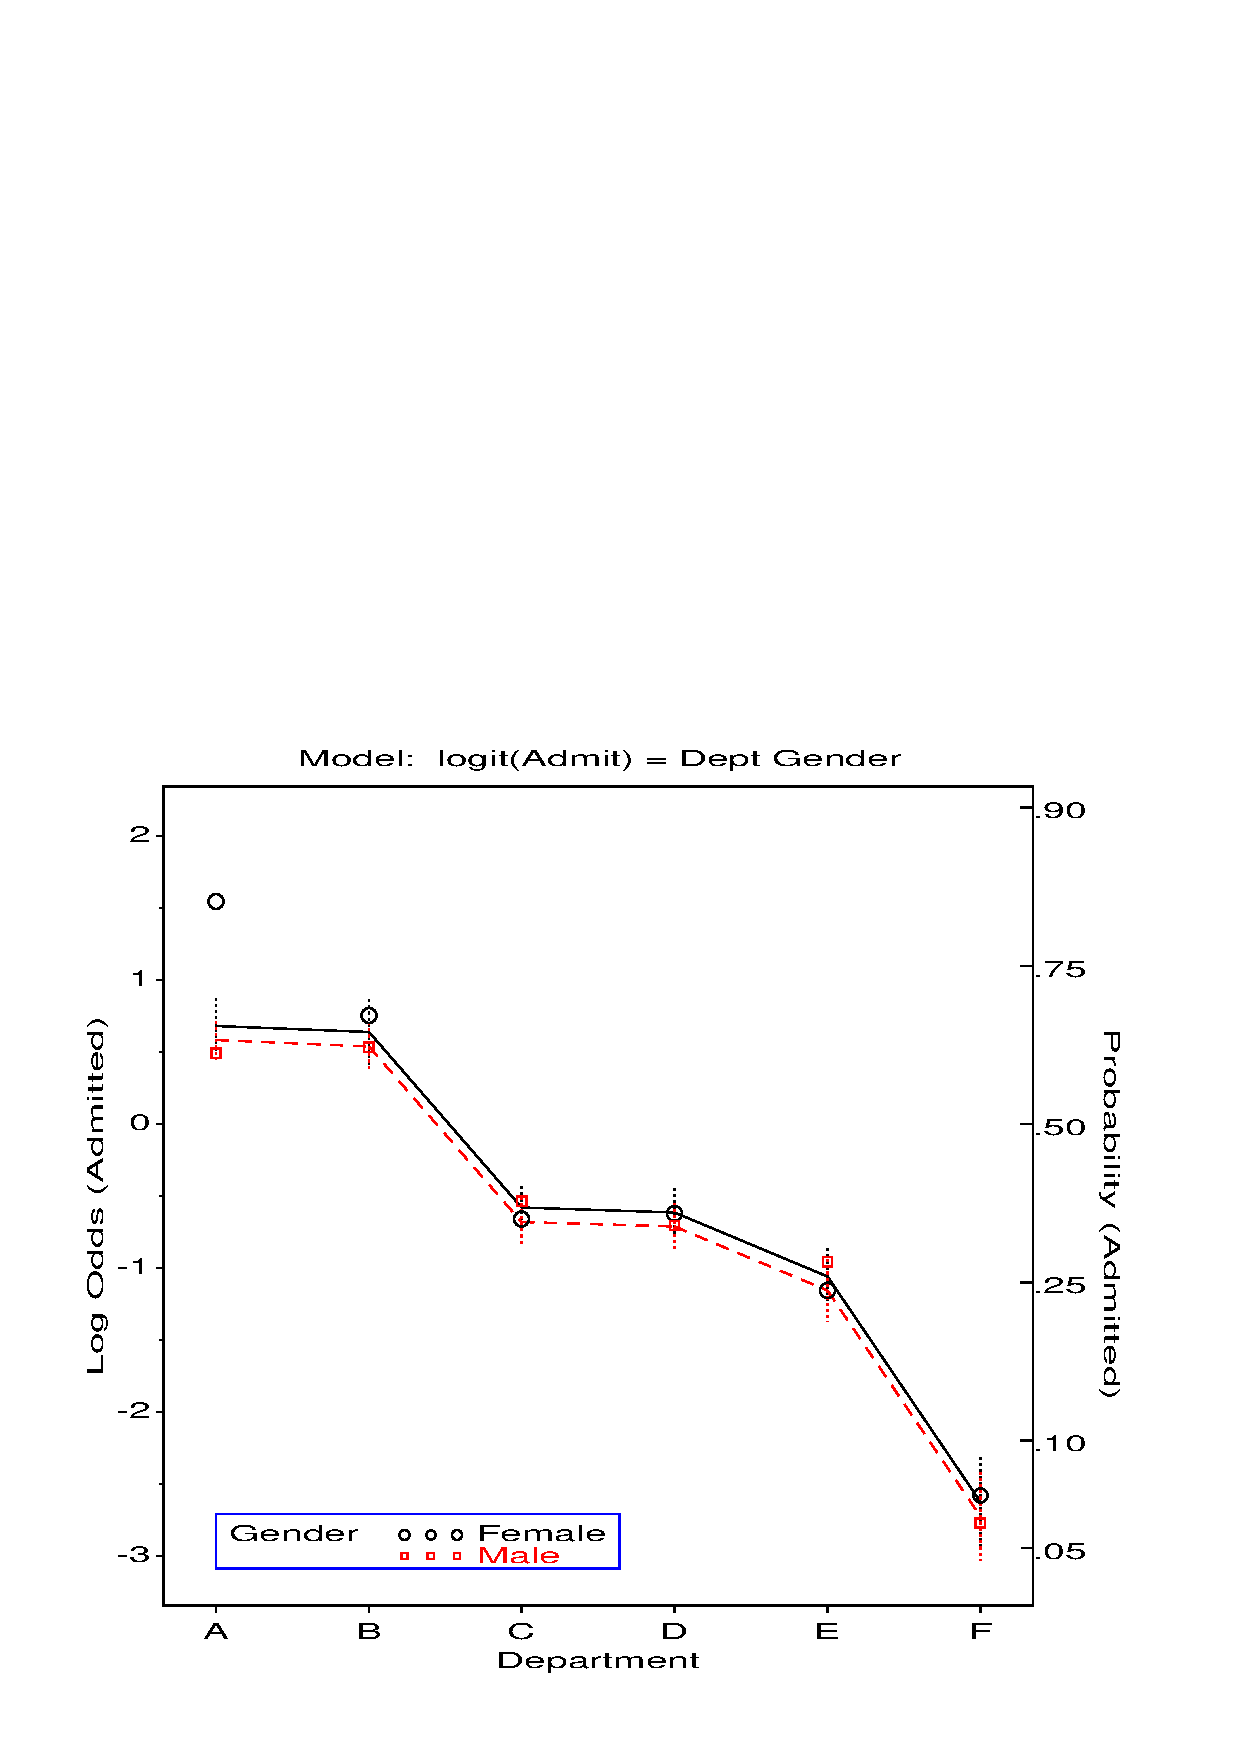
\includegraphics[scale=.6]{catberk2}
  \caption[Observed and fitted log odds of admission in the logit model]{Observed (points) and fitted (lines) log odds of admission in the logit model
  corresponding to [AD][AG][DG].  The error bars show individual 95\%
  confidence intervals around each fitted logit.}%
  \label{fig:catberk2}
\end{figure}

The statements below draw the plot of observed and predicted logits
(\verb|_type_='FUNCTION'|) shown in \figref{fig:catberk2}.
The \macro{PSCALE} constructs an \ADS\
which draws the probability values on the right vertical axis in the
plot.
The label for this axis is specified in the \stmt{TITLE}{GPLOT}, with
an angle, \pname{A=-90}, meaning the right-hand side, rotated \degree{90}.
By default, the macro uses the \pname{AXIS} and \pname{SYMBOL}
statements defined before the macro call.
Separate curves are
drawn for each level of the \pname{CLASS=GENDER} variable.
The values of the \pname{CLASS} variable may be labeled in the plot
or supplied in a \stmt{LEGEND}{CATPLOT}.
The parameter \pname{Z=1.96} specifies the multiple of
the standard error of the fitted logit (\verb|_SEPRED_|) used to
draw the error bars in the plot,
giving (asymptotic) 95\% individual confidence intervals.
\begin{listing}
%pscale(lo=-4, hi=3, anno=pscale, prob=%str(0.05,.1,.25,.5,.75,.9));

title h=1.6 'Model:  logit(Admit) = Dept Gender'
            a=-90 'Probability (Admitted)'
      h=3.5 a=-90 ' ';
legend1 position=(bottom inside left)  offset=(4,3)
        mode=share cborder=blue across=1
        shape=symbol(6,1.5) label=('Gender')
        value=(c=black 'Female'
               c=red   'Male');
axis1 order=(-3 to 2) offset=(4)
      label=(a=90 'Log Odds (Admitted)');
axis2 label=('Department') offset=(4);
symbol1 i=none v=circle h=1.7 c=black;
symbol2 i=none v=dot    h=1.7 c=red  ;
%catplot(data=predict,
   xc=dept, y=_obs_, class=gender,
   type=FUNCTION,
   z=1.96, anno=pscale, legend=legend1);
\end{listing}

The effects seen in our earlier analyses (Examples~\ref{ex:berkeley4}
and \ref{ex:berkeley4b})
may all be observed in this
plot.
The effect of gender is shown by the constant separation
between the two curves.
From the plot we see that this effect is very small and nonsignificant (compared
with the error bars).
If the gender effect were omitted from the model,
the fitted logits would be the same
for men and women applying to each department, and would plot as a curve
parallel to, but in between, the two shown in the graph.
Most of the observed points are quite close to their predicted values,
except in Department A,
where the probability of admittance for women is substantially
greater than that for men.
In \exref{ex:berkeley6} we dealt with this by allowing one extra parameter
for an association between admission and gender in department A,
giving the \loglin\ model \eqref{eq:berk2}.

We can see what this model ``looks like'' by recasting it in logit form.
The \loglin\ model \eqref{eq:berk2}
has an equivalent logit formulation, which also adds a 1 df term for an
effect of gender in department A,
\begin{equation}\label{eq:berk4}
  L_{ij} =
  \alpha   +  \beta _i^{\mbox{\scriptsize Dept}}
  +  \delta_{j=1} \beta^{\mbox{\scriptsize Gender}}
  \period
\end{equation}

This model may be fit
with \PROC{CATMOD} as shown below.  The association term between admission
and gender for Dept. A (\texttt{dept1AG}) is fit as a \pname{DIRECT}
variable.  The \pname{gender} variable is not included in the
\stmt{MODEL}{CATMOD}, so it must be listed in the
\stmt{POPULATION}{CATMOD}.
Because the \macro{CATPLOT}
uses the values in the \ODS, the plotting step is unchanged.

\begin{listing}
data berkeley;
   set berkeley;
   dept1AG = (gender='F') * (dept=1);

proc catmod order=data
            data=berkeley;
   weight freq;
   population dept gender;
   direct dept1AG;
   response / out=predict;
   model admit = dept dept1AG / ml noiter noprofile ;
%catplot(data=predict, xc=dept, class=gender, type=FUNCTION,
   z=1.96, legend=legend1);
\end{listing}

%% one figure
\begin{figure}[htb]
  \centering
  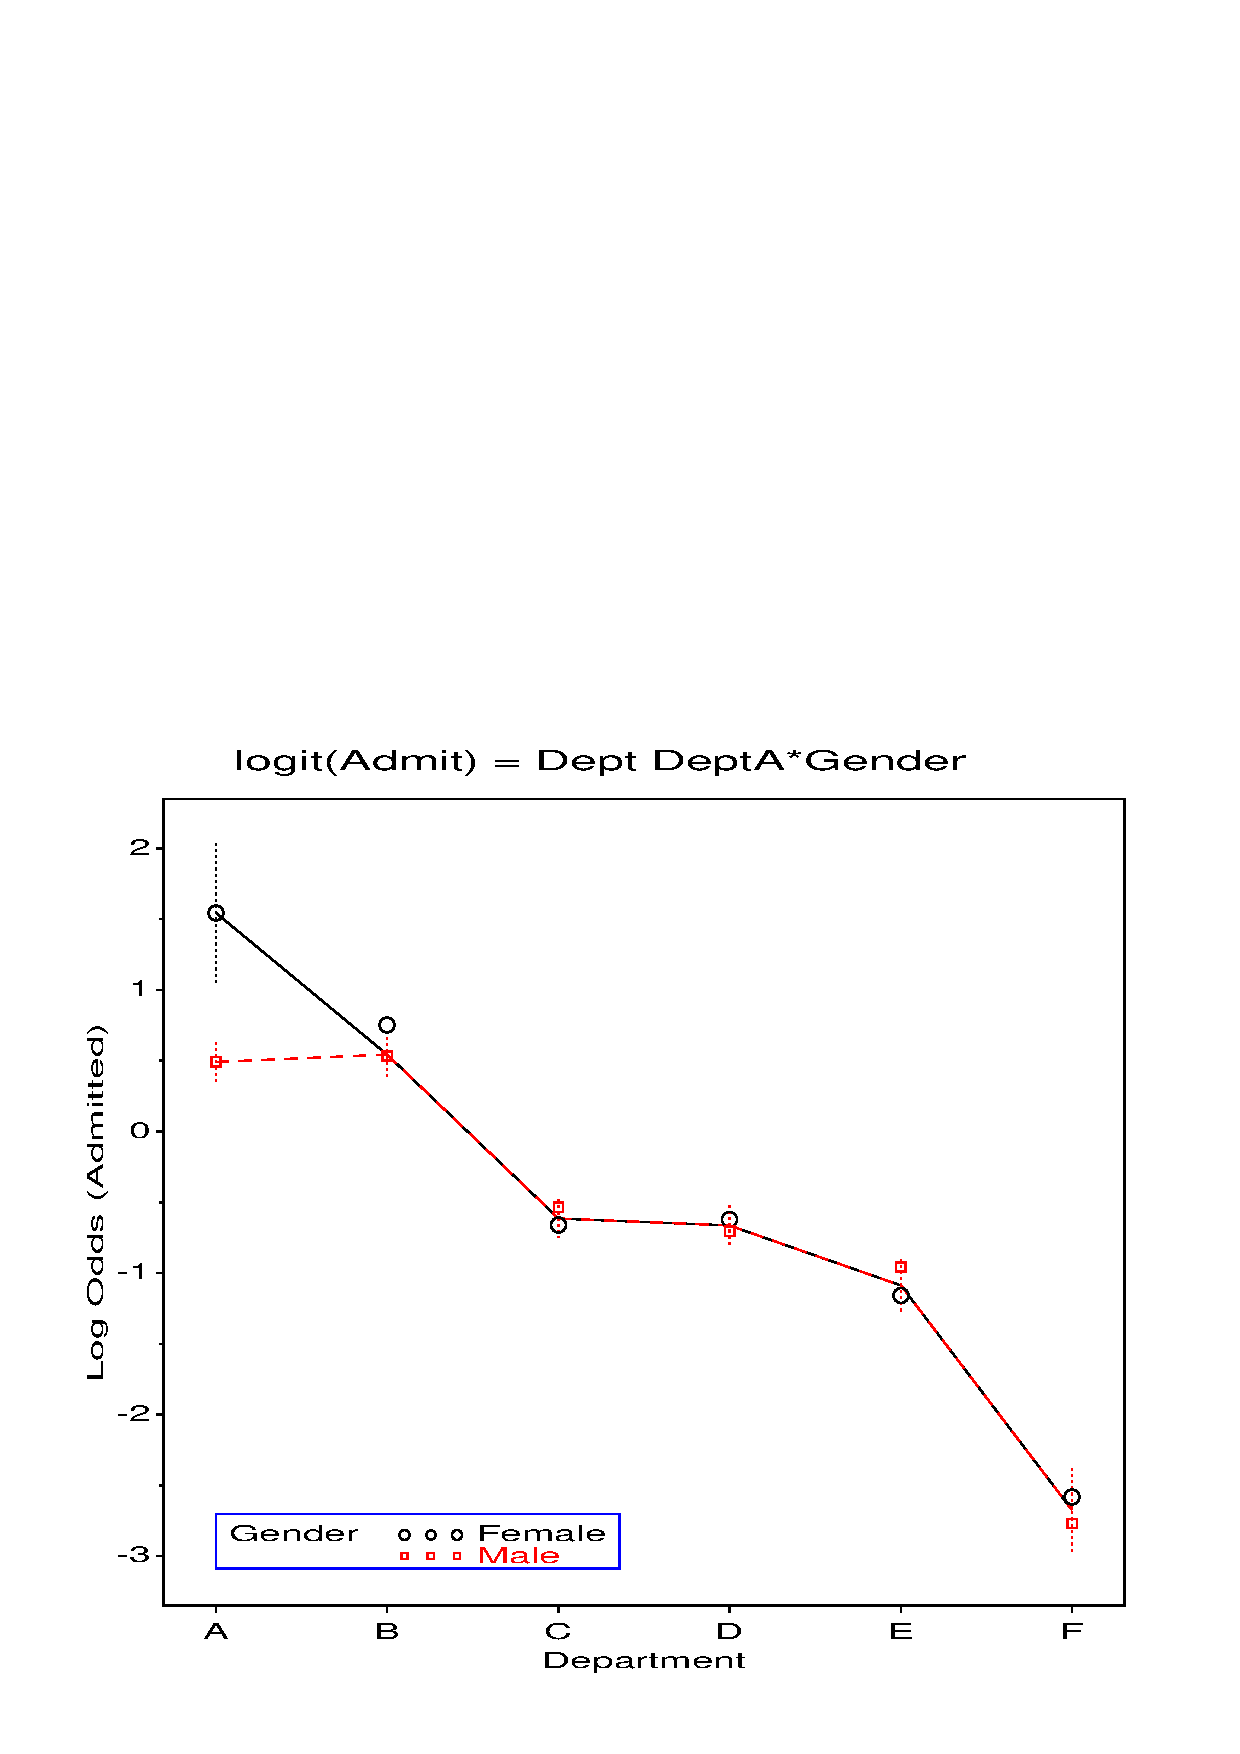
\includegraphics[scale=.6]{catberk6}
  \caption{Observed and fitted logits for model \eqref{eq:berk2}}%
  \label{fig:catberk6}
\end{figure}
The resulting plot for this model is shown in \figref{fig:catberk6}.
The graph gives a visual interpretation of the model
\eqref{eq:berk2} and its logit form, \eqref{eq:berk4}:
No effect of gender on admission, except in department A, where the
extra parameter allows perfect fit.
\end{Example}


\subsection{Zero frequencies}
Cells with frequencies of zero create problems for \loglin\ and logit
models.  For \loglin\ models, most of the derivations of expected
frequencies and other quantities assume $n_{ijk\cdots} > 0$.
In logit models, the observed log odds (e.g., for a three-way table),
$\log ( n_{ij1} / n_{ij2} )$, will be undefined if either frequency is
zero.

Zero frequencies may occur in \ctabs\ for two different reasons:
\begin{description}
\item[structural zeros] (also called \emph{fixed zeros}) will occur when it is impossible to observe
values for some combinations of the variables.
For example, suppose we have three different methods of contacting
people at risk for some obscure genetically inherited disease:
newspaper advertisement, telephone campaign, and radio appeal.
If each person contacted in any way is classified dichotomously
by the three methods of contact, there can never be a non-zero
frequency in the `No-No-No' cell.%
\footnote{Yet, if we fit an unsaturated model, expected frequencies
may be estimated for all cells, and provide a means to estimate
the total number at risk in the population.
See \citet[Section 5.4]{Lindsey:95}.}
\item[sampling zeros] (also called \emph{random zeros})
occur when the total size of the sample is not large enough in relation to the probabilities in each of the cells to assure that someone will be observed
in every cell.
For example, in a European survey of religious affiliation and occupation,
we may not happen to observe any Muslim vineyard-workers in France, although such individuals surely exist.
Even when zero frequencies do not occur, tables with many cells relative to
the total frequency tend to produce small expected frequencies in at
least some cells, which tends to make  the \chisq\ statistics for model fit
and Wald statistics for individual terms unreliable.
\end{description}

\PROC{CATMOD} takes a simple approach to distinguishing these two cases:
Cells with zero frequency are simply deleted from the \ctab,
and thus are treated as structural zeros.  To avoid this, some corrective
action is needed.
One solution (for sampling zeros) is to collapse categories of some variables,
but we are often loath to do this for fear of loss of information.

Other suggestions are:
\begin{seriate}
\item Add a small positive quantity (0.5 is usually recommended) to every
cell in the \ctab\ \citep{Goodman:70}, as is done in calculating
empirical log odds (\secref{sec:logist-logodds});
\PROC{CATMOD} provides the \opt{ADDCELL}{CATMOD} in the \stmt{MODEL}{CATMOD} for this purpose,
but this option is ignored for maximum likelihood estimation.
\item Replace sampling zeros by some small number, typically
$10^{-10}$ or smaller \citep{Agresti:90}.
\item Add a small quantity, like 0.1, to all zero cells
\citep{EversNamboodiri:77}.
\end{seriate}

\begin{Example}[reagan]{Race and politics in the 1980 US Presidential vote}
\tabref{tab:reagtab} shows data (\citet[Table 4.12]{Agresti:90}, from \citet{CloggShockey:88})
from the 1982 General Social Survey on
votes in the 1980 US Presidential election for Reagan or for Carter
or other in relation to race and conservatism (1=most liberal,
7=most conservative).
The \Dset\ \pname{vote}, containing the
variables \pname{race}, \pname{cons}, \pname{votefor}, and
\pname{count} is listed in \datref{dat:vote}.

\begin{table}[htb]
 \caption{1982 General Social Survey: Reagan vs. Carter, by Race and Conservatism}\label{tab:reagtab}
 \begin{center}
 \begin{tabular}{c rr rr}
  \hline
       & \multicolumn{4}{c}{Race} \\
  Political & \multicolumn{2}{c}{White} & \multicolumn{2}{c}{Non White} \\ 
  \cline{2-5}
  Conservatism & Reagan & Carter/other  & Reagan & Carter/other \\ 
  \hline
  1 & 1 & 12 & 0 & 6 \\ 
  2 & 13 & 57 & 0 & 16 \\ 
  3 & 44 & 71 & 2 & 23 \\ 
  4 & 155 & 146 & 1 & 31 \\ 
  5 & 92 & 61 & 0 & 8 \\ 
  6 & 100 & 41 & 2 & 7 \\ 
  7 & 18 & 8 & 0 & 4 \\ 
  \hline
 \end{tabular}
 \end{center}
\end{table}


It is natural to treat vote for Reagan vs. (Carter or other) as the response,
and race and conservatism as predictors in this $2 \times 2 \times 7$
table, with variables VoteFor ($V$), Race ($R$) and Conservatism ($C$).
Before fitting models, it is useful to take an exploratory look
at the data.
The fourfold display shown in \figref{fig:reagan1a}
shows separate panels for each level of conservatism.
In order to focus on the tendency to vote for Reagan vs.\ (Carter or other)
among Whites compared to Non Whites,
the number of White and Non White respondents were equated in each
panel in this figure.
With this standardization confidence rings will overlap in the left
and right quadrants ( Reagan vs.\ Carter or other) when the (conditional)
odds ratio
does not differ significantly from 1.

%% one figure
\begin{figure}[htb]
  \centering
  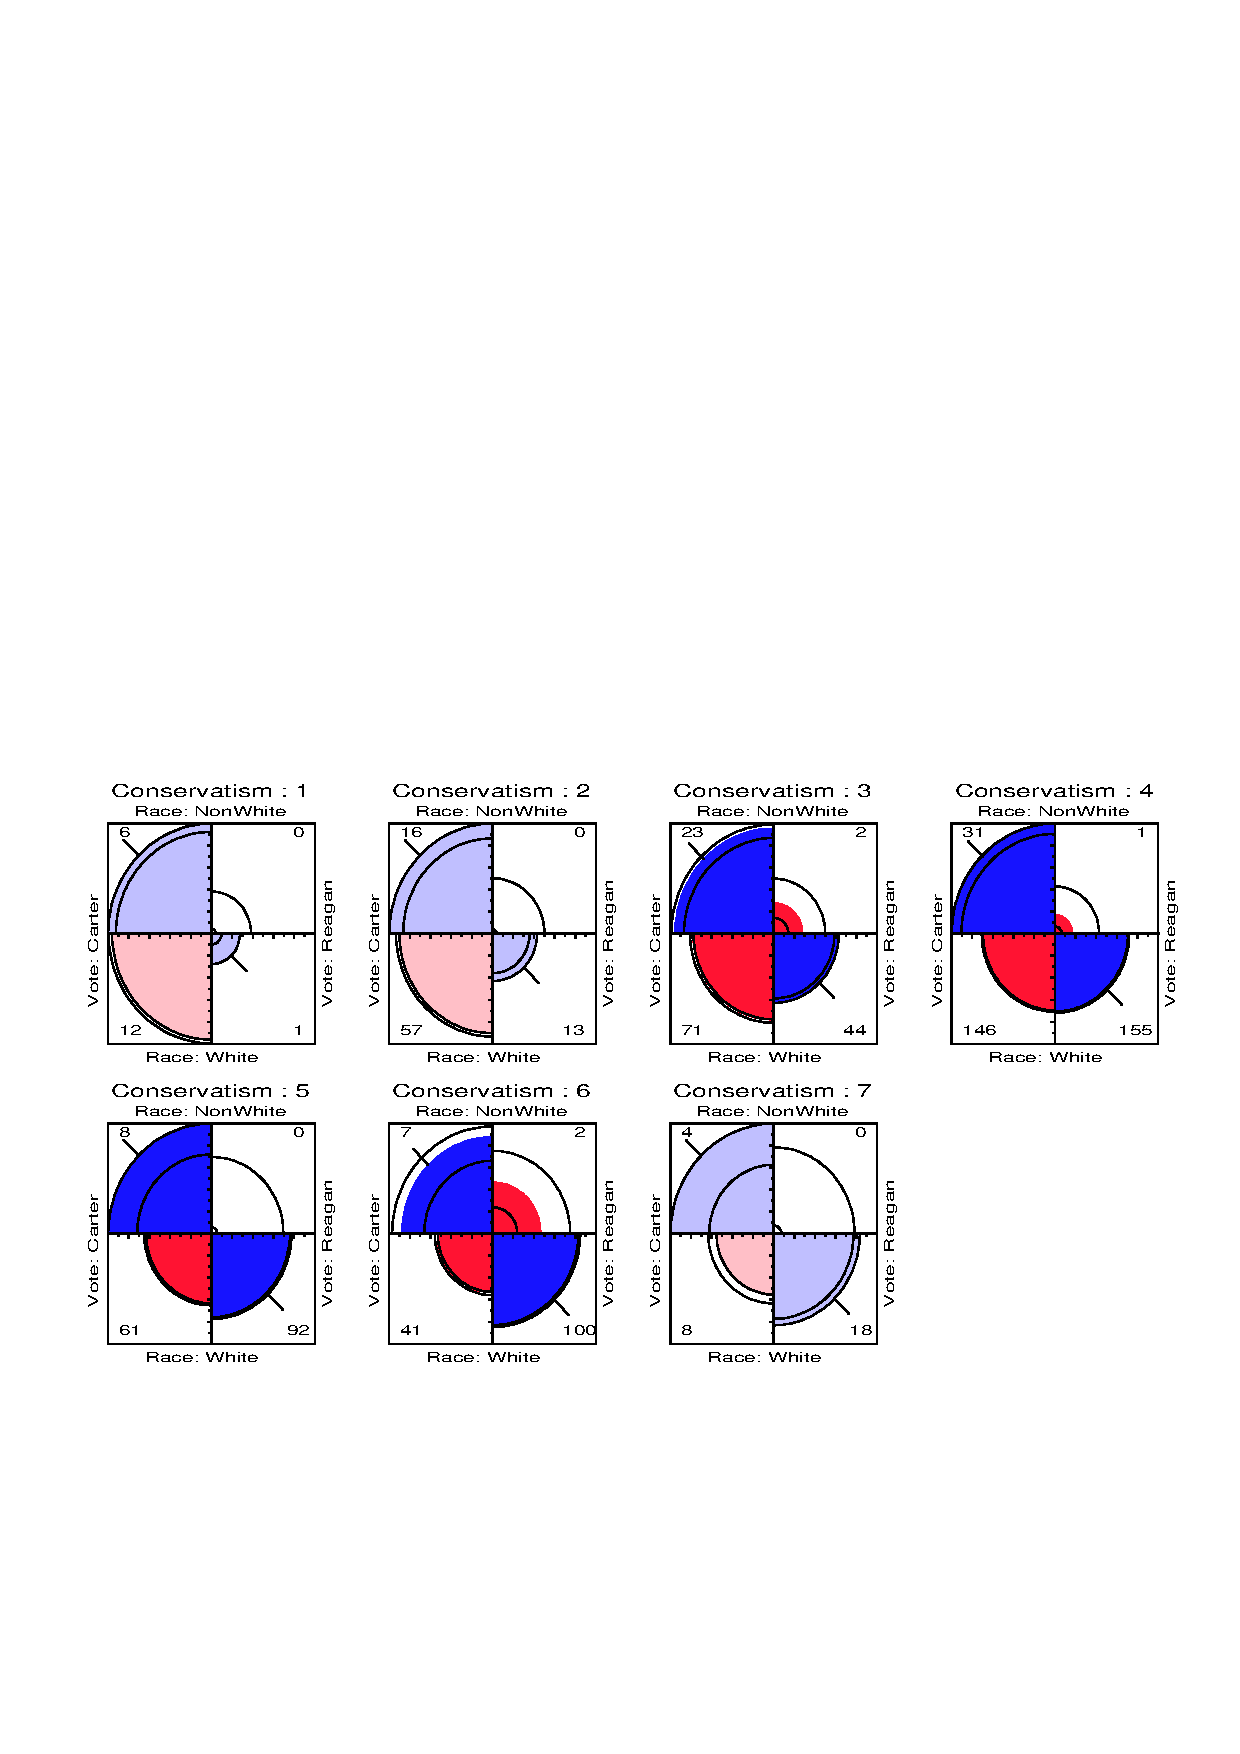
\includegraphics[width=\textwidth,clip]{reagan1a}
  \caption[Fourfold display for Vote, by Race and Conservatism]{Fourfold display for Vote, by Race and Conservatism, equating the number of White and Non White respondents at each level of Conservatism}%
  \label{fig:reagan1a}
\end{figure}

Thus, among Whites, in the bottom half of each panel,
we may compare the areas of the left and right quadrants,
and see that the propensity to vote for Reagan increases with
conservatism.
A similar trend is evident among Non White respondents, but there
are a number of zero frequencies here, among Non Whites who indicated they
voted for Reagan.

The conditional odds ratios for Vote and Race given Conservatism are all in the same direction, indicating that Whites were more likely to vote for
Reagan at \emph{any} level of Conservatism.
The \sasprog{fourfold}  gives the test of homogeneity of odds ratios
shown in \outref{out:reagan1.1},
which is equivalent to a test for lack-of-fit of the
homogeneous association \loglin\ model $[RC] [VR] [VC]$.
The tests of conditional independence, $V \perp R \given C$,
suggest that voting preference depends on race, and possibly conservatism.

\ixon{zero cells}
To illustrate the problem of zero cells, consider tests of fit of the
saturated model, $[RCV]$, and of the homogeneous association model,
$[RC] [VR] [VC]$, fit as \loglin\ models under three conditions:
\begin{seriate}
\item no adjustment for zeros,
\item replace zeros by $10^{-10}$, and
\item add 0.5 to each cell.
\end{seriate}
In each case, the models are fit
with the statements below, after possible adjustment to the \pname{count}
variable.
The results are summarized in \tabref{tab:reagzero}.
\begin{listing}
proc catmod data=vote;
   weight count;
   model cons*race*votefor = _response_ / ml noiter noresponse noprofile;
   loglin cons|race|votefor / title='Saturated model';
  run;
   loglin cons|race|votefor @2 / title='No 3-way association';
\end{listing}
In case (a), the four zero cell are treated as structural zeros, and
deleted, leaving only 2 df for the test of lack-of-fit in the
no-3-way model.
In case (b), the main effect parameter for Race cannot be estimated
and there is, paradoxically, 1 df for the test of the saturated model.
Case (c), adding 0.5 to each cell, has no anomalies, and we adopt this
solution for this example. In other cases it is recommended to compare
several approaches to determine if any conclusions are affected by
the presence of zero cells.
\ix{zeros!structural}

\begin{table}[htb]
 \caption{Effects of zero-cell actions on \loglin\ models for \pname{vote} data}\label{tab:reagzero}
 \begin{center}
 \begin{tabular}{l rrrr}
  \hline
   \multicolumn{1}{r}{Model:}  & \multicolumn{2}{c}{$[RCV]$} & \multicolumn{2}{c}{$[RC] [VR] [VC]$} \\
  Action                     & df & \GSQ\ & df & \GSQ\ \\ 
  \hline
(a)  None                       & 0 & . & 2 & 1.89 \\ 
(b)  $n=0 \rightarrow 10^{-10}$ & 1 & 0.00 & 6 & 4.96 \\ 
(c)  $n	\rightarrow n+\frac12$ & 0 & . & 6 & 3.45 \\ 
  \hline
 \end{tabular}
 \end{center}
\end{table}

\ixoff{zero cells}

\begin{Output}[htb]
\caption{Vote data: Test of Homogeneity of odds ratios}\label{out:reagan1.1}
\small
\verbatiminput{ch7/out/reagan1.1}
\end{Output}

We proceed to fit a main effects logit model.
Treating the vote for Reagan vs. Carter or other as the response, the
logit model with nominal main effects for race and conservatism is

\begin{equation} \label{eq:logrnom}
    \logit ( \mbox{Reagan} / \mbox{Carter} )  =
    \alpha   +
    \beta _i^{\mbox{\scriptsize Race}}  +
    \beta _j^{\mbox{\scriptsize Cons}}
	 \period
\end{equation}
Model \eqref{eq:logrnom} may be fit with \PROC{CATMOD} as follows. \begin{listing}
data vote;
    set vote;
    count = count + 0.5;
proc catmod data=vote order=data;
   weight count;
   response / out=predict;
   model votefor = race cons / noiter noresponse noprofile;
\end{listing}

The model fit statistics and parameter estimates for the logit model
\eqref{eq:logrnom} are shown in \outref{out:glogit1.1}.
The model fits quite well.
\begin{Output}[htb]
\caption{Vote data: Fit of the nominal main effects model}\label{out:glogit1.1}
\small
\verbatiminput{ch7/out/glogit1.1}
\end{Output}

To interpret the model, we plot the observed and predicted logits, with
90\% confidence intervals, as shown below.  The \macro{CATPLOT}
gives \figref{fig:glogit11}.
\begin{listing}
%pscale(lo=-5, hi=2.3, anno=pscale, prob=%str(0.01,.05,.1,.25,.5,.75,.9));

axis1 order=(-5 to 2) offset=(0,3)
      label=(a=90 'Logit (Reagan / Carter)');
axis2 label=('Conservatism') offset=(2);
symbol1 i=none v=circle h=1.9 c=black;
symbol2 i=none v=square h=1.7 c=red  ;
legend1 position=(bottom inside center) offset=(,2);
%catplot(data=predict, class=race, x=cons, z=1.65, anno=pscale,
   legend=legend1);
\end{listing}

%% one figure
\begin{figure}[htb]
  \centering
  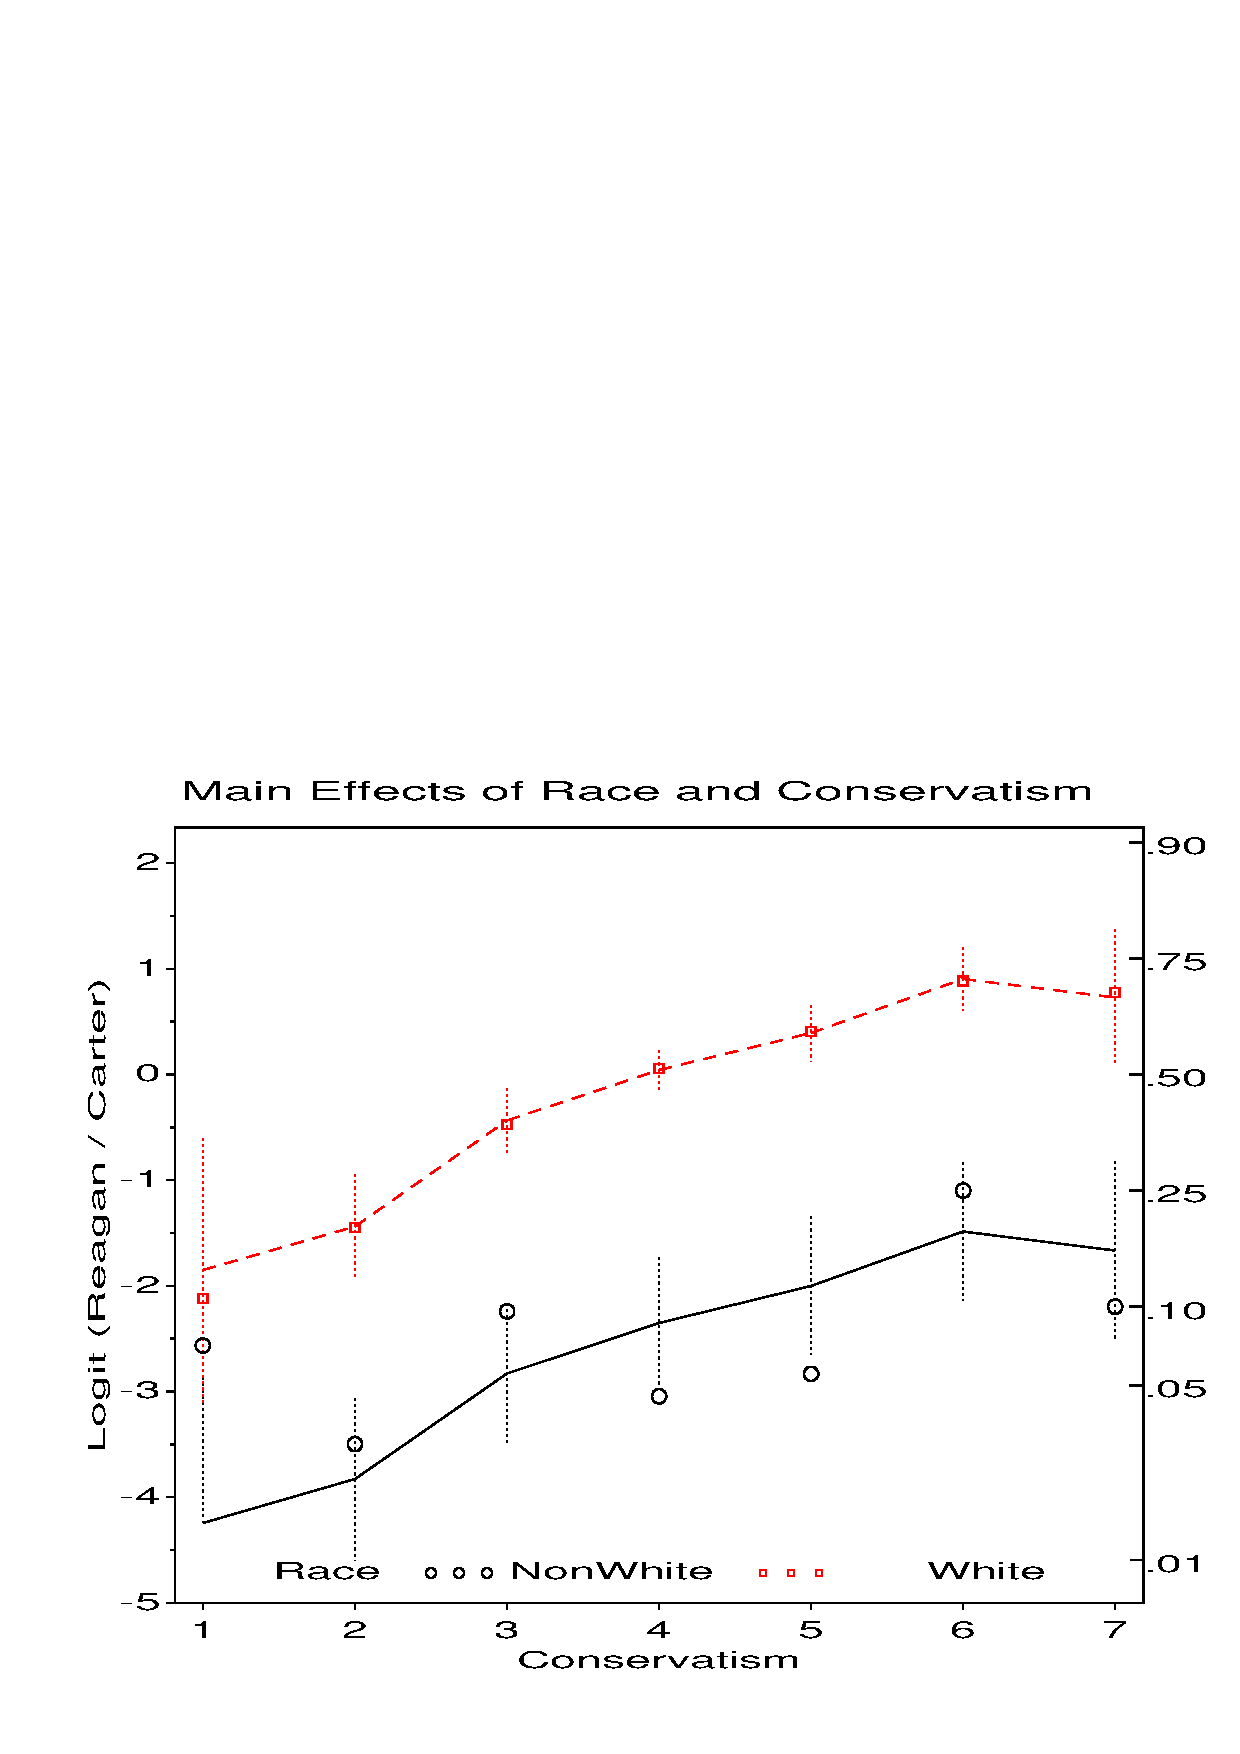
\includegraphics[scale=.6]{glogit11}
  \caption[Observed and fitted logits for main effects model]{Observed (points) and fitted (lines) logits for main effects model.  Dotted lines show a 90\% confidence interval around the predicted log odds.}%
  \label{fig:glogit11}
\end{figure}
Notice that for both Whites and Non Whites, the log odds of voting for
Reagan increases with conservatism.  This is also reflected in the
parameter estimates for \pname{cons} in \outref{out:glogit1.1},
which increase in approximately equal steps.
Model \eqref{eq:logrnom} does not use the ordinal nature of conservatism.
A model which uses conservatism as a direct,
quantitative independent variable ($c$) can be expressed as

\begin{equation} \label{eq:logrlin}
  \mbox{logit ( Reagan / Carter )}  =
  \alpha   +
  \beta _i^{\mbox{\scriptsize Race}}  +
  \beta ^{\mbox{\scriptsize Cons}} \,  c
\end{equation}
Note that there is just one parameter for conservatism,
$ \beta ^{\mbox{\scriptsize Cons}}$, which is interpreted as
an increase in the log odds of a vote for Reagan for each
change of 1 unit in conservatism.
Model \eqref{eq:logrlin} may be fit with \PROC{CATMOD}
just by adding the statement \pname{DIRECT CONS;}
\begin{listing}
proc catmod data=vote order=data;
   direct cons;
   weight count;
   response / out=predict;
   model votefor = race cons / noiter noresponse noprofile ;
   title 'Linear Effect for Conservatism' h=2.5 a=-90 ' ';
\end{listing}
The \LR\ \GSQ\ for this model is $\GSQ (11) = 9.58$, and
the difference in \GSQ\ for Models
\eqref{eq:logrlin} and \eqref{eq:logrnom} is
$\Delta \GSQ (5) = 6.13$,
so the linear model cannot be rejected, given that the nominal
model fits.  The estimate $\widehat{\beta} ^{\mbox{\scriptsize Cons}} = 0.472$
indicates that the odds of voting for Reagan increase by a factor of
$\exp(0.472) = 1.60$ (60\%) for each step of increasing conservatism.

%\begin{Output}[htb]
%\caption{}\label{out:glogit1.2}
%\small
%\verbatiminput{ch7/out/glogit1.2}
%\end{Output}

The observed and fitted logits are plotted exactly as before, using
the same \macro{CATPLOT} call with the new \ODS\ \pname{predict}.
The plot is shown in \figref{fig:glogit12}.
Note that the 90\% confidence limits around predicted values are
noticeably smaller than in \figref{fig:glogit11}.
This is but one advantage of models for ordinal variable,
which we discuss in the following section.
%% one figure
\begin{figure}[htb]
  \centering
  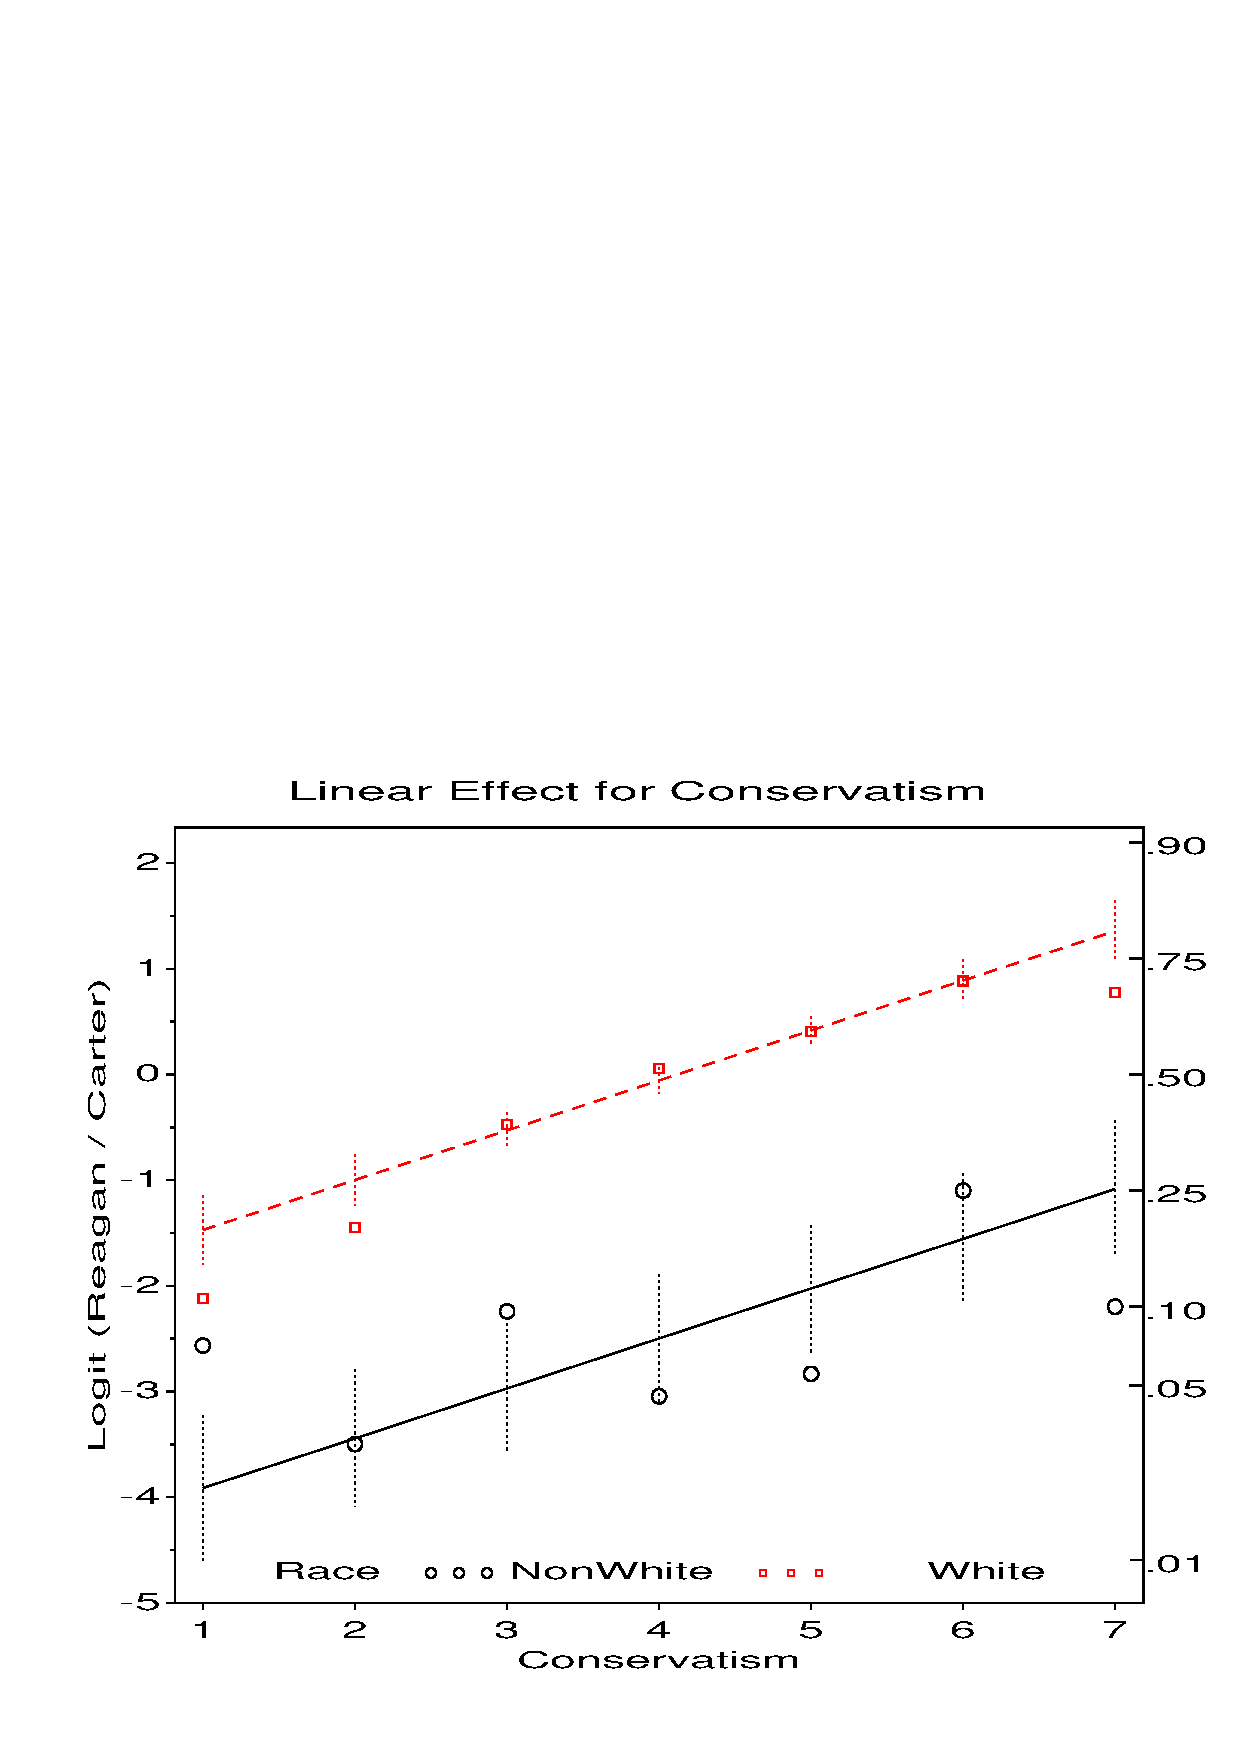
\includegraphics[scale=.6]{glogit12}
  \caption[Observed and fitted logits for linear effect of conservatism]{Observed (points) and fitted (lines) logits for linear effect of conservatism.  Dotted lines show a 90\% confidence interval around the predicted log odds.}%
  \label{fig:glogit12}
\end{figure}
\end{Example}


\section{Models for ordinal variables}\label{sec:loglin-ordinal}
Standard \loglin\ models treat all classification variables as
nominal, unordered factors;
all statistical tests are identical
and parameter estimates are equivalent
if the categories of any variable are reordered.
Yet we have seen that the ordering of categories often provides
important information about the nature of associations
and we showed (\secref{sec:ordinaltests}) that non-parametric
tests which take into account the ordered nature of a factor
are more powerful.

In a mosaic display, an ordered associative effect is seen when
the residuals have an opposite-corner pattern of positive and negative
signs and magnitudes (e.g., for the hair-eye color data,
\figref{fig:mosaic34} or the Titanic data, \figref{fig:mostitanic1}).
In a correspondence analysis plot,
an association has an ordered effect when the points for two factors are
ordered similarly.
In these cases \loglin\ and logit models which use the ordered nature of the factors
offer several advantages.
\begin{itemize}
\item Because they are more focused, tests which use the ordinal
structure of the table variables are more powerful when the association
varies systematically with the ordered values of a factor.

\item Because they consume fewer degrees of freedom,
we can fit unsaturated models where the corresponding model for
nominal factors would be saturated.
In a two-way table, for example, a variety of models for ordinal
factors may be proposed which are intermediate between the independence
model and the saturated model.

\item Parameter estimates from these models are fewer in number, and are
easier to interpret, and quantify the nature of effects better
than corresponding quantities in models for nominal factors.
Estimating fewer parameters typically gives smaller standard errors,
as we saw in \exref{ex:reagan}.
\end{itemize}
These advantages are analogous to the use of tests for trends or
polynomial effects in ANOVA models.

Models for ordinal variables may be specified in \loglin\ form,
as described in \secref{sec:loglin-ordlog}.  When there is an ordinal
response variable, related models may be specified in terms of
logits for adjacent categories (\secref{sec:loglin-ordadj}),
or cumulative logits (\secref{sec:loglin-ordcum}).
The descriptions here are brief. For further information refer to
\citet{Agresti:84}, \citet[Ch. 9]{Agresti:90} and
\citet{Goodman:79,Goodman:83}.

\subsection{Loglinear models for ordinal variables}\label{sec:loglin-ordlog}
For a two-way table, when either the row variable or the column variable,
or both, are ordinal, one simplification comes from assigning ordered
scores, $\{a_i\}, a_1 \le a_2 \le \cdots a_I$, and/or
$\{b_j\}, b_1 \le b_2 \le \cdots b_J$
to the categories
so that the ordinal relations are necessarily included in the model.
Typically, equally spaced scores are used, for example, integer
scores, $\{a_i\}=i$, or the zero-sum equivalent, $\{a_i\}=i-(I+1)/2$
(e.g., $\{a_i\}= \{-1, 0, 1\}$ for $I=3$).
These give simple interpretations of the
association parameters in terms of \emph{local odds ratios},
\begin{equation*}
 \theta_{ij} =
 \frac{ m_{ij} \: m_{i+1, j+1} } { m_{i,j+1} \: m_{i+1, j} }
 \comma
\end{equation*}
the odds ratio for adjacent rows and adjacent columns.

When both variables are assigned scores, we have the \glossterm{linear-by-linear model},
\begin{equation}\label{eq:linlin}
\log ( m_{ij} ) = \mu  +  \lambda_i^A
+  \lambda_j^B  +  \gamma \: a_i b_j \period
\end{equation}
Because the scores are fixed, this model has only one extra parameter, $\gamma$, compared to the
independence model, which is the special case, $\gamma=0$.
The terms  $\gamma a_i b_j $ describe a pattern of association
where deviations from independence increase linearly with $a_i$
and $b_j$ in opposite directions towards the opposite corners of
the table.

In the linear-by-linear association model, the local log odds ratios
are
\begin{equation*}
\log \theta_{ij} =
 \gamma (a_{i+1} - a_i) (b_{j+1} - b_j)
 \comma
\end{equation*}
which reduces to
\begin{equation*}
\log \theta_{ij} =
 \gamma
\end{equation*}
for integer-spaced scores, so $\gamma$ is the common local log odds ratio.
As a result, the linear-by-linear model is sometimes called the
model of \emph{uniform association} \citep{Goodman:79}.
\ix{uniform association model}
\ix{linear-by-linear model}
\ix{log odds ratio!local}

Generalizations of the linear-by-linear model result when only one
variable is assigned scores.
In the \glossterm{row-effects model},
the row variable, say, $A$ is treated as nominal, while
the column variable, $B$, is assigned ordered scores $\{b_j\}$.
The \loglin\ model is then
\begin{equation}\label{eq:roweff}
 \log ( m_{ij} ) = \mu  +  \lambda_i^A
  +  \lambda_j^B  +  \alpha_i b_j
 \comma
\end{equation}
where the $\alpha_i$ parameters are the \emph{row effects}.
An additional constraint,
$\sum_i \alpha_i =0$ or $\alpha_I =0$
 is imposed, so that model \eqref{eq:roweff}
has $(I-1)$ more parameters than the independence model.
The linear-by-linear model is the special case where the row effects
are equally spaced, and the independence model is the special case
where all $\alpha_i = 0$.

The row-effects model \eqref{eq:roweff} also has a simple odds ratio interpretation.
The local log odds ratio for adjacent pairs of rows and columns is
\begin{equation*}
\log \theta_{ij} =
  \alpha_{i+1} - \alpha_i
  \comma
\end{equation*}
which is constant for all pairs of adjacent columns.  Plots of the
local log odds ratio against $i$ would appear as a set of parallel
curves.

In the analogous \glossterm{column-effects model}, $(J-1)$ linearly independent
column effect
parameters $\beta_j$ are estimated for the column variable, while fixed
scores $\{a_i\}$ are assigned to the row variable.

The linear-by-linear model \eqref{eq:linlin} and the row-effects model
\eqref{eq:roweff} can be fit using \PROC{CATMOD},
but to do so requires that you enter the complete model matrix explicitly.
With \PROC{GENMOD} you need only create a numeric variable with score
values in the input \Dset, a much easier task.
\begin{Example}[mental2]{Mental impairment and parents' SES}
In \exref{ex:mental1} \CA\ was used to explore the relationship between
ratings of the mental health status of young New Yorkers and
their parents' socioeconomic status (SES).
\figref{fig:correses} showed that most of the association in the
table was accounted for by a single dimension along which both factors
were ordered, consistent with the view that mental health increased
in relation to parents' SES.

For comparison, we first fit the independence model with both
\PROC{CATMOD} and \PROC{GENMOD}.
As we expect, this model fits quite badly,
with $\GSQ\ (15) = 47.418$.
\begin{listing}
%include catdata(mental);
proc catmod data=mental;
   weight count;
   model mental*ses = _response_ / noiter noprofile noresponse;
   loglin mental ses / title='Independence';
   run;
\end{listing}
For illustration, the standardized (adjusted) deviance residuals,
$g_i / \sqrt ( 1 - h_i )$
are obtained in the \PROC{GENMOD}
step (named \pname{stresdev} in the \pname{obstats} \Dset),
and used with the \macro{MOSAIC} to produce the mosaic
display shown in the left panel of \figref{fig:mental2}.%
\footnote{To ensure that the the levels of both factors are ordered
correctly, \pname{MENTAL} and \pname{SES} were entered as numeric
variables in the \Dset\ \pname{MENTAL}, and user-formats were used
to provide the character labels shown in \figref{fig:mental2}.
Because \IML\ does not make use of formatted values, the \macro{TABLE}
was used to convert the numeric variables to character.
}
The parameter \pname{cellfill=dev 0.5}
causes the program to write the value of all residuals greater than 0.5
in absolute value in the corresponding tile.
\begin{listing}
proc genmod data=mental;
   class mental ses;
   model count = mental ses / dist=poisson obstats residuals;
   make 'obstats' out=obstats noprint;
run;

%table(data=mental, var=Mental SES, weight=count, char=Y,
       format=mental mental. ses ses., order=data, out=mental2);
data obstats;
   merge mental2 obstats;
%mosaic(data=obstats, vorder=Mental SES, plots=2, split=H V, resid=stresdev,
   title=Mental Impairment and SES: Independence, cellfill=dev 0.5);
\end{listing}
%% two subfig side-by-side
\begin{figure}[htb]
 \begin{minipage}[t]{.49\linewidth}
  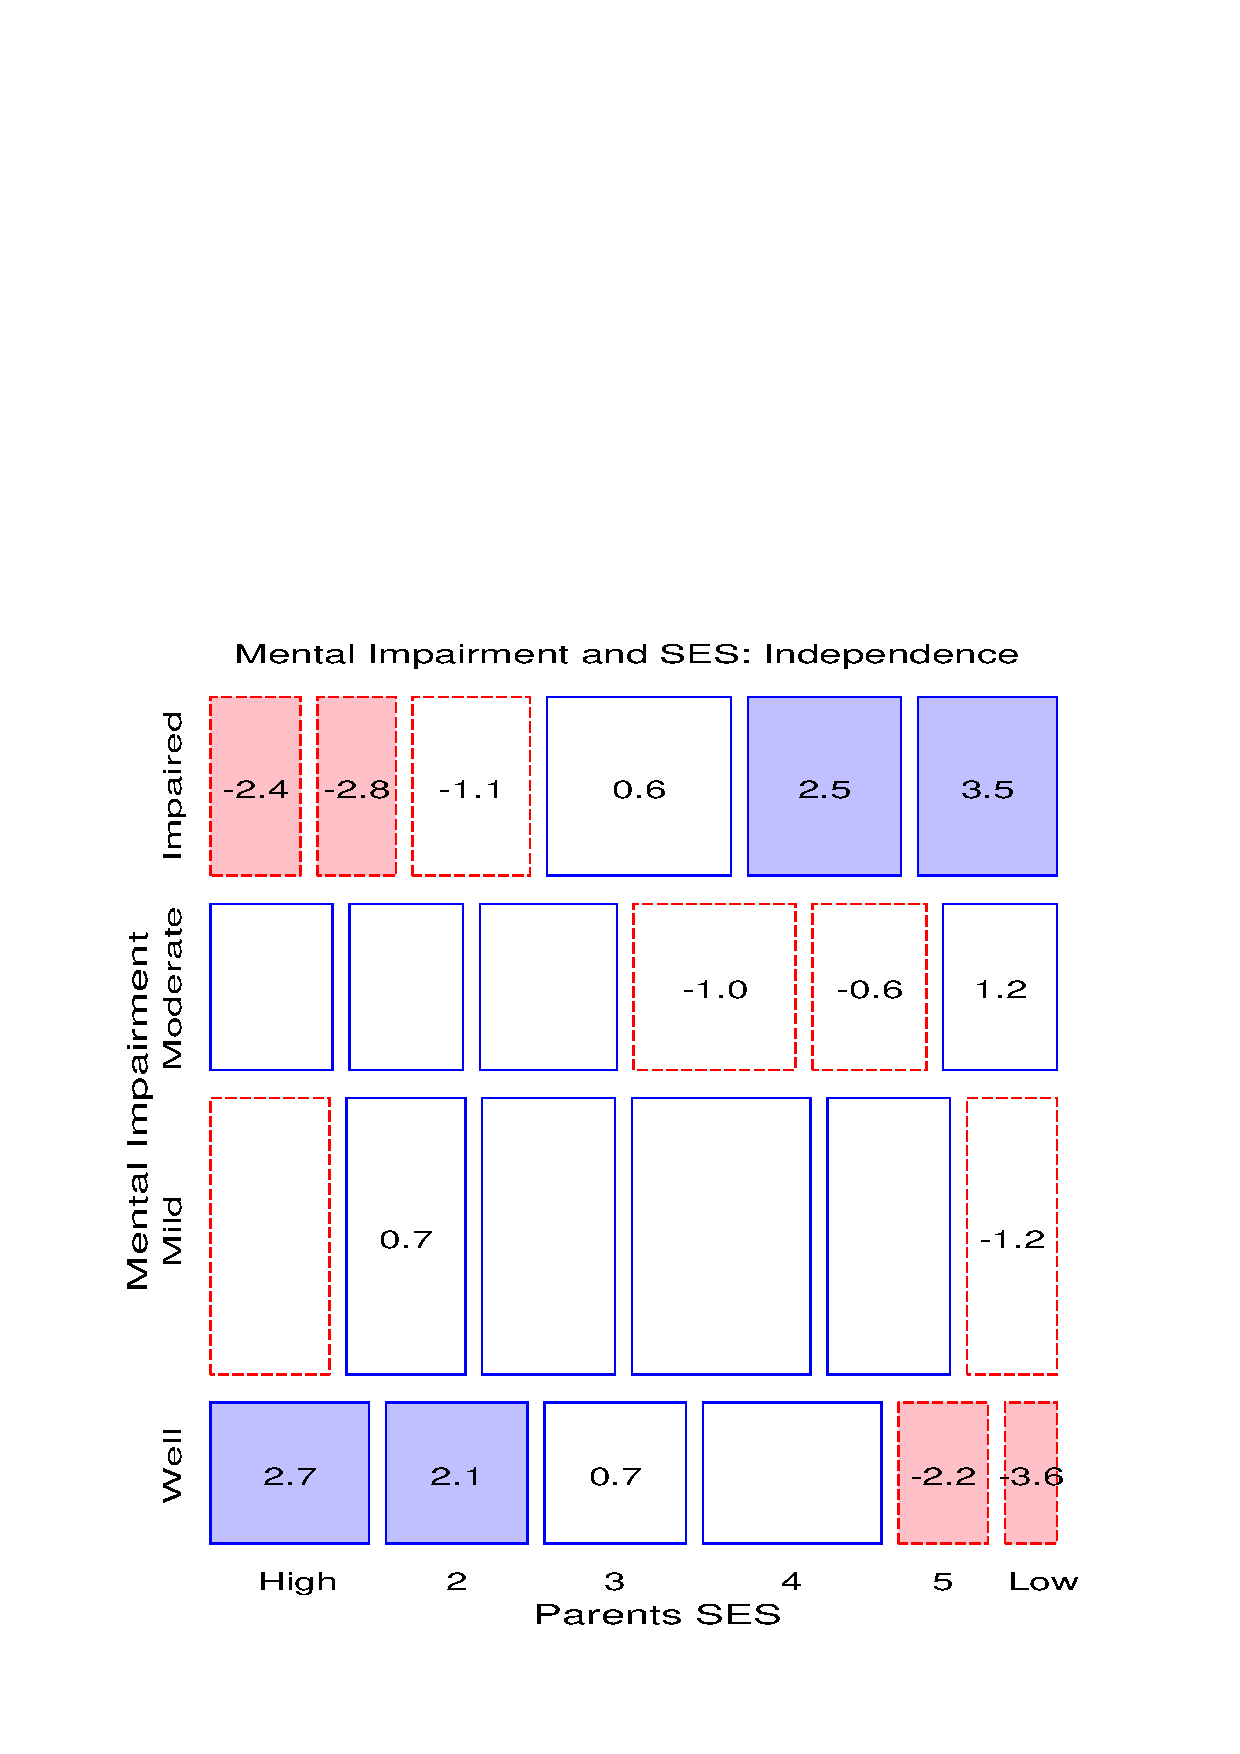
\includegraphics[width=1\linewidth]{mental21}
 \end{minipage}%
 \hfill
 \begin{minipage}[t]{.49\linewidth}
  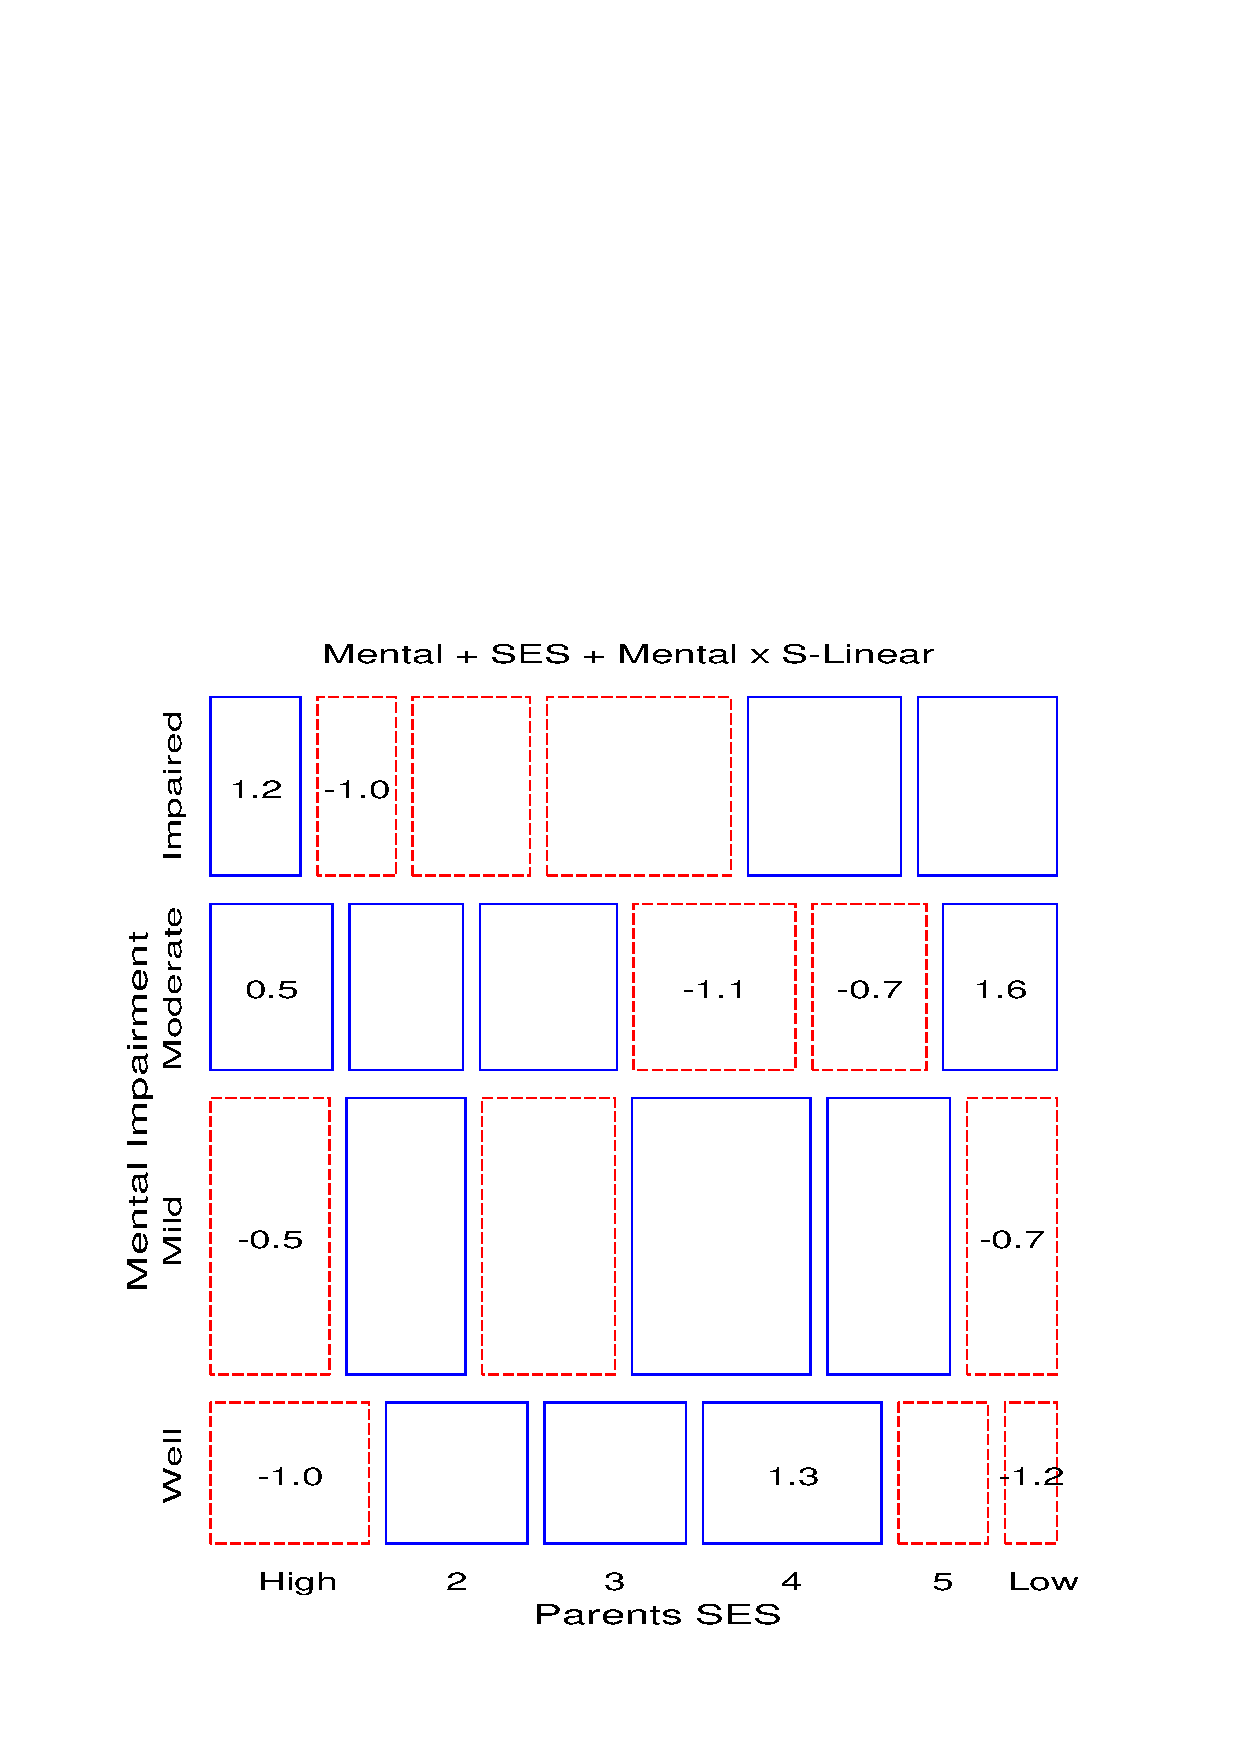
\includegraphics[width=1\linewidth]{mental22}
 \end{minipage}
 \caption[Mental health and SES: Residuals]{Mental health and SES: Residuals from Independence (left) and Row Effects (right) Models}\label{fig:mental2}
\end{figure}
Note that the residuals in \figref{fig:mental2} for the
independence model have the opposite-corner pattern which would
arise if either the row-effects model (with ordered row effects)
or the linear-by-linear
association model described the association between mental health
and SES.
\begin{table}[htb]
 \caption{Mental health data: Goodness-of-fit statistics for ordinal \loglin\ models}\label{tab:mentab2}
 \begin{center}
 \begin{tabular}{l rrrr r}
  \hline
  Model                & df & $\chisq$ & $\GSQ$ & $\Delta \GSQ$  & AIC \\ 
  \hline
  Independence         & 15 & 45.985 & 47.418 & .    &  17.42\\ 
  Linear-by-linear     & 14 & 9.732 & 9.895 & 37.523 & -18.18\\ 
  Row-effects (Mental) & 12 & 6.289 & 6.281 & 41.137 & -17.72\\ 
  \hline
 \end{tabular}
 \end{center}
\end{table}



To fit models in which the association terms for \pname{mental} and/or
\pname{ses} use quantitative scores, create copies, \pname{M} and
\pname{S} of these variables.  They are used as quantitative variables
when they appear in the \stmt{MODEL}{GENMOD}, but are \emph{not} listed
as \pname{CLASS} variables.
The following statements fit the row-effects model, using SES
as a linear effect, and then the linear-by-linear model.
Goodness-of-fit statistics for all three models are shown in
\tabref{tab:mentab2}.

\begin{listing}
data mental;
   set mental;
   m = mental;    *-- copy m and s as quantitative, non-class;
   s = ses;

title 'Linear SES';
proc genmod data=mental;
   class mental ses;
   model count = mental ses mental*s / dist=poisson obstats residuals;
   make 'obstats' out=obstats noprint;
run;
data obstats;
   merge mental obstats;
%mosaic(data=obstats, var=Mental SES, resid=stresdev,  split=H V,
   title=Mental + SES + Mental x S-Linear, cellfill=dev 0.5);

title 'Linear x Linear';
proc genmod data=mental;
   class mental ses;
   model count = mental ses m*s / dist=poisson obstats residuals;
run;
\end{listing}
The $\Delta \GSQ$ values in \tabref{tab:mentab2} each test whether
the corresponding model results in a significant reduction in the
residual $\GSQ$ compared to the independence model.  Both are
highly significant.

Similarly, the difference in $\GSQ$ between the linear-by-linear
and row-effects model, $\Delta \GSQ\ (2) = 9.732-6.289 = 3.443$ suggests that the 
row-effects model
is \emph{not} a significant improvement over the
linear-by-linear model.
The AIC values suggest a slight preference for the linear-by-linear model.
The residuals for the row effects model are shown in the right
panel of \figref{fig:mental2}; residuals for the linear-by-linear
model (not shown) have the same signs, but are slightly smaller
in some cells.

\begin{Output}[htb]
\caption{Parameter estimates for the row-effects \loglin\ model, Mental health data}\label{out:mental2.1}
\small
\verbatiminput{ch7/out/mental2.1}
\end{Output}

Under the linear-by-linear model, the estimate of the coefficient of
\pname{M*S} is $\hat{\gamma} = 0.0907$ (s.e.=0.015) with unit-spaced scores.
This corresponds to a local odds ratio, $\hat{\theta}_{ij} = \exp (0.0907) = 1.095$.
This single number describes the association succinctly:
each step down socioeconomic scale increases the odds of being classified
one step poorer in mental health by 9.5\%.

Parameter estimates for the row-effects model are shown in
\outref{out:mental2.1}.  The row effects are the values of
the \pname{S*MENTAL} terms.  These values are ordered, consistent with
mental health status having ordinal associative effects,
but (with integer scores for both variables) they are not equally
spaced, as the linear-by-linear model would imply.
The spacing of these parameter estimates is similar to what we saw
in the \CA\ plot (\figref{fig:correses}), with the middle categories
Mild Impairment, and Moderate Impairment relatively close together
compared to the extreme categories.

These \loglin\ models and the associated mosaic displays do not
provide a clear preference between the row-effects and linear-by-linear
models here.
We turn now to other models and graphical displays which may distinguish them better.
\end{Example}


\subsection{Adjacent category logit models}\label{sec:loglin-ordadj}
When there is a single response variable, logit models provide a
simple way to model the dependence of the response on the other,
explanatory variables.  For an ordinal response,
models for the logits between adjacent response categories
allow the ordered nature of the response to be taken into account.
For the model of independence, the \emph{adjacent category logits} are
\begin{eqnarray}
A_{j| i} \equiv
\log \left(
 \frac{ \pi_{j+1|i} } { \pi_{j|i} }
 \right) =
\log \left(
 \frac{ m_{i, j+1} } { m_{ij} }
 \right)
  & = &
( \mu  +  \lambda_i^A +  \lambda_{j+1}^B ) -
( \mu  +  \lambda_i^A +  \lambda_j^B )  \nonumber \\
  & = &  \lambda_{j+1}^B -  \lambda_{j}^B \label{eq:aindep}
\end{eqnarray}
which are constants, say, $\beta_j = (\lambda_{j+1}^B -  \lambda_{j}^B )$
not depending on the explanatory variable(s).
If an explanatory variable is also ordinal, we may use scores, $\{a_i\}$
as before.
The analog of the linear-by-linear model with unit-spaced scores
allows the value of $A_{j| i}$ to vary linearly with the quantitative value,
\begin{equation}\label{eq:alin}
A_{j| i} = \beta_j + \gamma \: a_i
\end{equation}
The slope parameter $\gamma$ has a similar log odds interpretation:
the log odds of a response in category $j+1$
as opposed to category $j$ increases by $\gamma$
for each unit increase in the explanatory variable.
% The intercept parameters, $\beta_j$ ...

In a similar way, the fixed scores $a_i$ may be replaced by row effect
parameters, $\alpha_i$ to be estimated (with the constraint $\sum_i \alpha_i =0$ or $\alpha_I =0$)
to give the row-effects adjacent logit model
\begin{equation}\label{eq:arow}
A_{j| i} = \beta_j + \alpha_i
\end{equation}
A plot of the fitted logits against $i$ for this model appears as parallel
curves (rather than parallel lines under the linear-by-linear model
\eqref{eq:alin}).

Even less restrictive models, which are still unsaturated, may be fit if the row-effects model fits poorly.  For example, each adjacent logit may be
linearly related to an assigned score for an explanatory variable,
but the slopes may differ over the adjacent response categories
(the \emph{linear-interaction model}):
\begin{equation}\label{eq:alin-int}
A_{j| i} = \beta_j + \gamma_j \: s_i \period
\end{equation}
Alternatively, a quadratic relation between the
adjacent logits, $A_{j| i}$ and the scores,
$A_{j| i} = \beta_j + \gamma_1 \: a_i + \gamma_2 a_i^2$
may be fit.
These possibilities are illustrated below.

\begin{Example}[mental4]{Mental impairment and parents' SES}
We consider here adjacent category logit models for the Mental Health
data, treating \pname{MENTAL} as an ordinal response.
Adjacent logit models are easily fit with \PROC{CATMOD}
using the \pname{RESPONSE ALOGIT;} statement.
Differences among the logits for adjacent categories (the intercepts, $\beta_j$, in models \eqref{eq:alin} and \eqref{eq:arow}) are
specified by the \verb|_RESPONSE_| keyword in the
\stmt{MODEL}{CATMOD}.  Nominal explanatory variables are included
as main effects (and possibly, interactions) on the left-hand side
of the \stmt{MODEL}{CATMOD}.  An explanatory variable is treated
as quantitative when declared in a \stmt{DIRECT}{CATMOD}.

The following statements fit a series of adjacent category logit models
to the Mental Health data.  Model 0 has only a \verb|_RESPONSE_|
effect, and is analogous to the independence model.
In Model 1, the adjacent logits for mental impairment are affected
by SES, as a nominal variable.
Model 2 is the linear-by-linear model for adjacent logits, with
SES as a direct variable,
while Model 3 allows different slopes for each adjacent logit.
%% input: /users/faculty/friendly/sasuser/catdata/mental4.sas
%% last modified: 01-Dec-98 12:07
\begin{listing}
%include catdata(mental);

*-- Adjacent logit models;
proc catmod data=mental;
   weight count;
   population ses;
   response alogit / out=pred0;
   model mental = _response_ / noprofile noresponse title='Model 0:  _R_';
  run;
   response alogit / out=pred1;
   model mental = _response_  ses / noprofile noresponse title='Model 1: _R_ SES';
  run;
   direct ses;
   response alogit / out=pred2;
   model mental = _response_  ses / noprofile noresponse title='Model 2: _R_ S';
  run;
   direct ses;
   response alogit / out=pred3;
   model mental = _response_ | ses / noprofile noresponse title='Model 3: _R_|S';
  run;
\end{listing}

%% two subfig side-by-side
\begin{figure}[htb]
 \begin{minipage}[t]{.49\linewidth}
  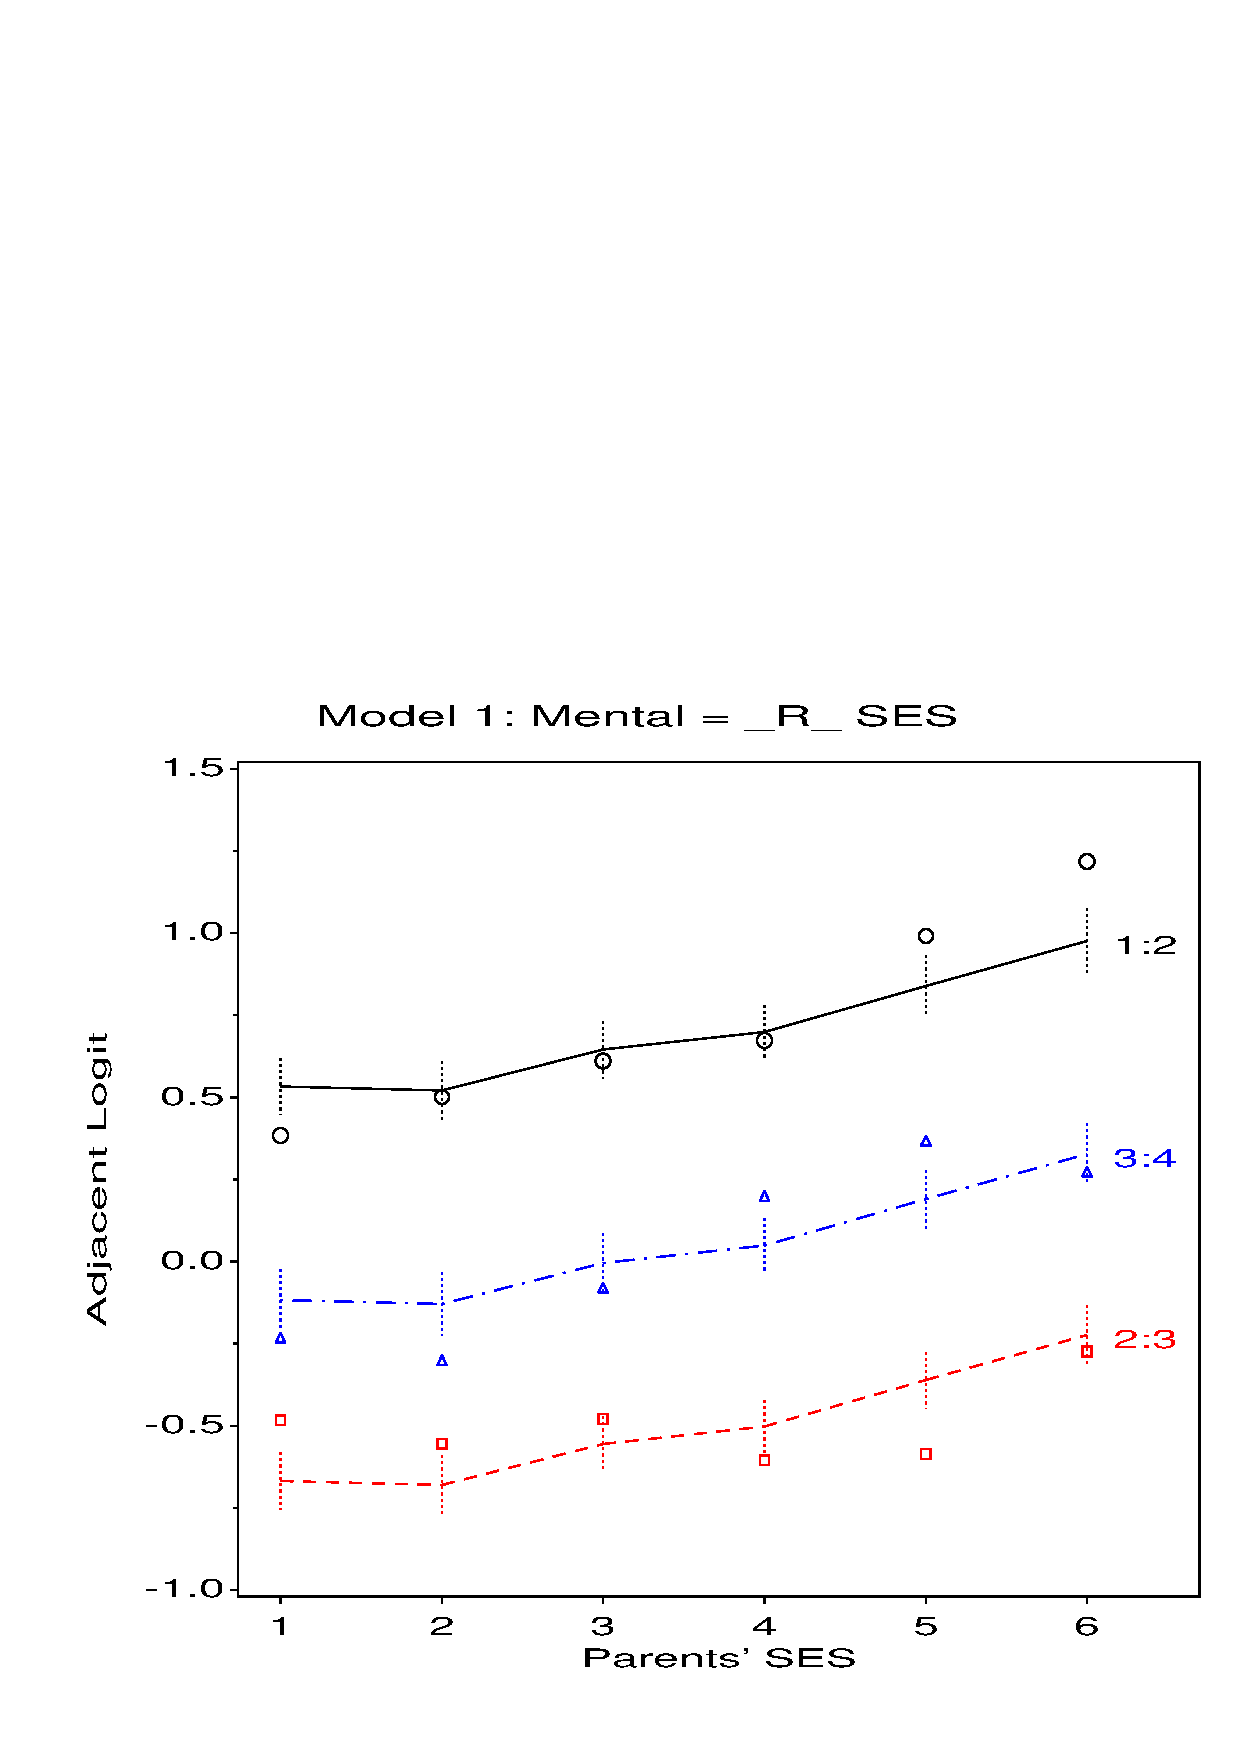
\includegraphics[width=1\linewidth]{mental41}
 \end{minipage}%
 \hfill
 \begin{minipage}[t]{.49\linewidth}
  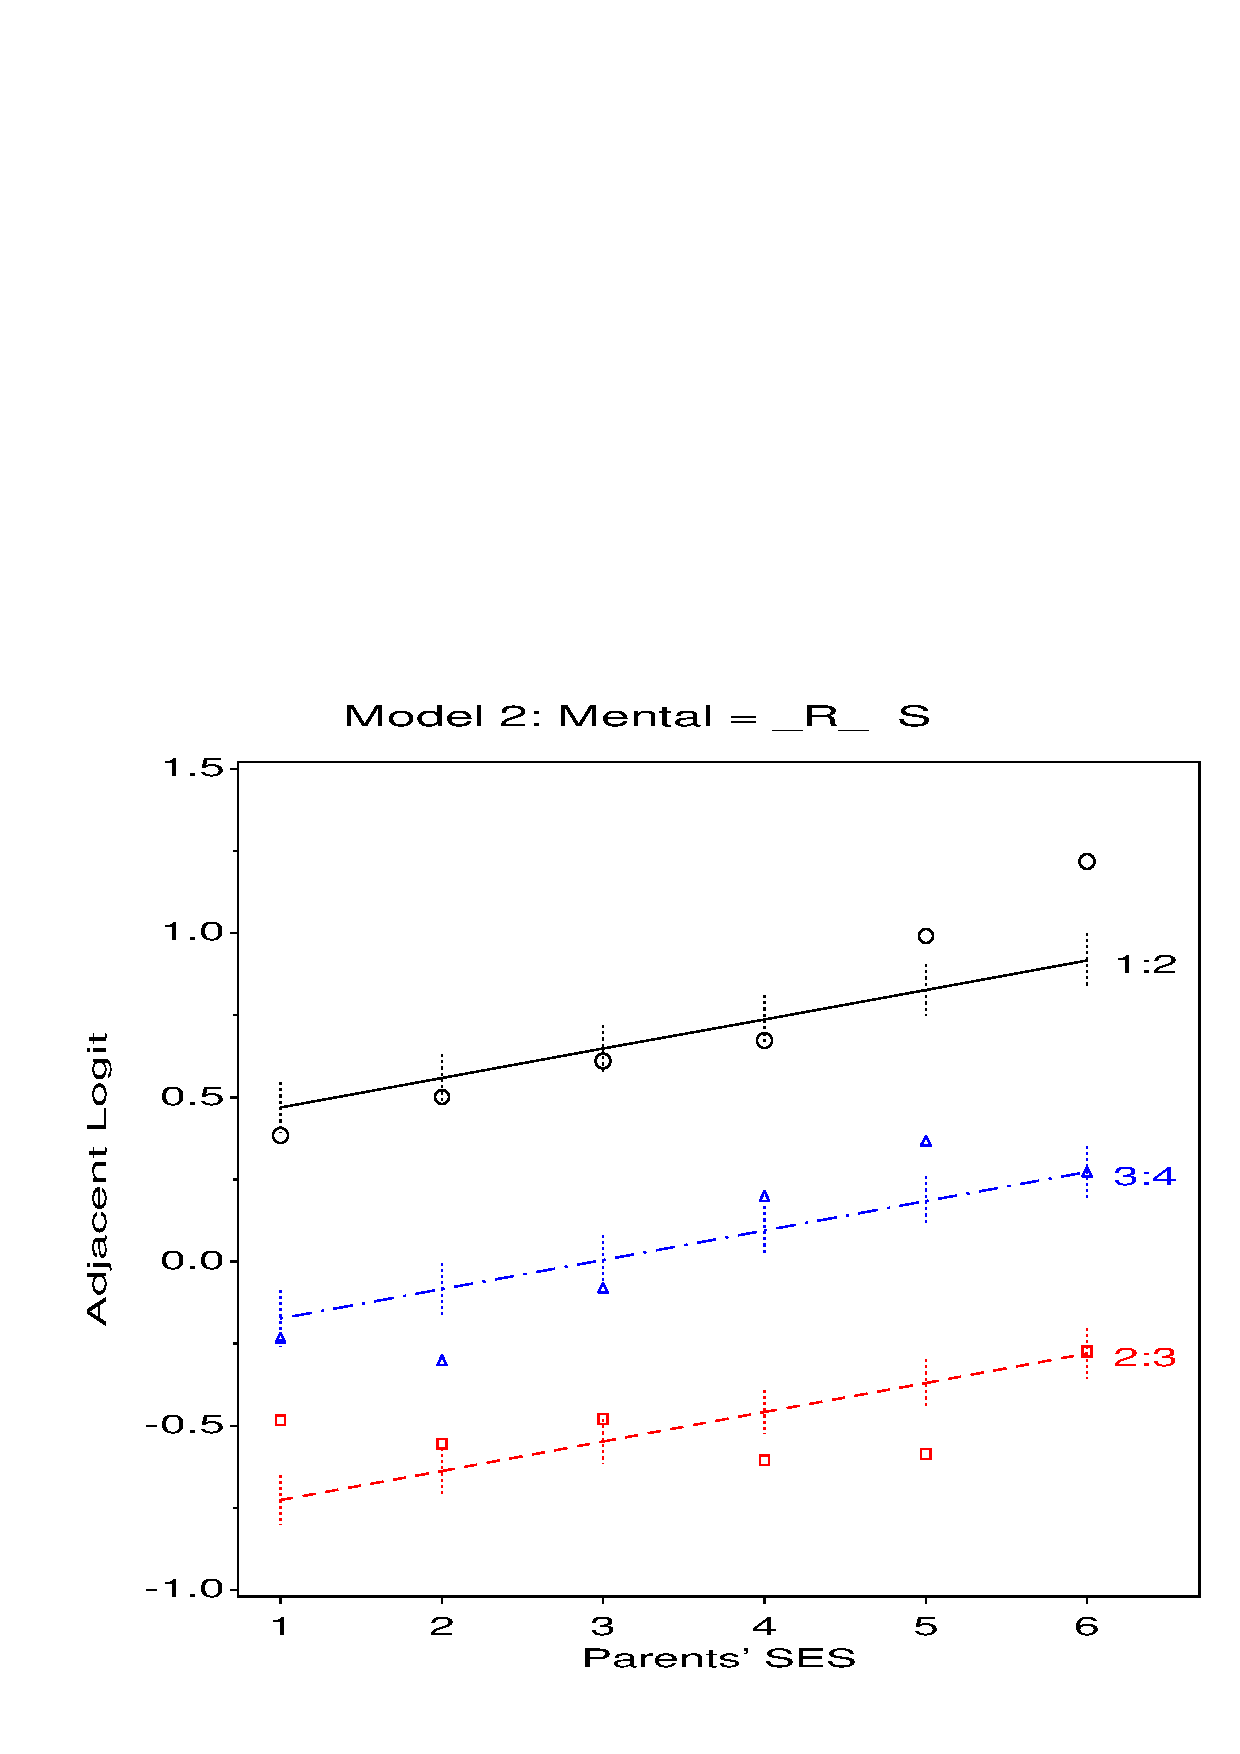
\includegraphics[width=1\linewidth]{mental42}
 \end{minipage}
 \caption{Adjacent category logit models for Mental Health data, Model 1 and Model 2}\label{fig:mental4a}
\end{figure}
\begin{table}[htb]
 \caption{Adjacent category logit models for Mental Health data}\label{tab:mentab4}
 \begin{center}
 \renewcommand{\arraystretch}{1.1}
 \begin{tabular}{c ll rrr r}
  \hline
  Model & Formula & Terms & df & \chisq\ & $p$-value & AIC\\ 
  \hline
  0 & $A_{j| i} = \beta_j $                  & \verb\_R_\     & 15 & 44.35 & 0.0001 & 14.35\\ 
  1 & $A_{j| i} = \beta_j + \alpha_i$        & \verb\_R_ SES\ & 10 & 6.76 & 0.7478  & -13.24\\ 
  2 & $A_{j| i} = \beta_j + \gamma \: a_i$   & \verb\_R_ S\   & 14 & 9.68 & 0.7849  & -18.32\\ 
  3 & $A_{j| i} = \beta_j + \gamma_j a_i$    & \verb\_R_|S\   & 12 & 6.26 & 0.9023 & -17.74\\ 
  4 & $A_{j| i} = \beta_j + \gamma_1 a_i + \gamma_2 a_i^2$ & \verb\_R_ S S^2\ & 13 & 7.39 & 0.8809 & -18.61\\ 
  5 & $A_{j| i} = \beta_j + \gamma_j a_i + \delta a_i^2$ & \verb\_R_|S S^2\ & 11 & 3.69 & 0.9782 & -18.69\\ 
  \hline
 \end{tabular}
 \end{center}
\end{table}

For each model, an \ODS, which contains the observed and fitted logits,
is requested with the \opt{OUT=}{CATMOD} in the \stmt{RESPONSE}{CATMOD}.
Plotting the observed and fitted logits
makes it easy to see what relationships are implied by each model.
The plots for Model 1 and Model 2, shown in \figref{fig:mental4a},
are produced with the \macro{CATPLOT}
as shown below.
The macro call requests a plot of the observed logit
(\verb|_OBS_|) against \pname{SES}, with separate curves for each
adjacent logit (\verb|CLASS=_NUMBER_|).
By default, the macro also draws curves connecting the predicted
values (\verb|_PRED_| in the \ODS) and $\pm 1$ standard error bars
around each fitted logit.
\begin{listing}
axis1 label=(a=90) order=(-1 to 1.5 by .5);
axis2 offset=(3,8);
proc format;
   value cum 1='1:2'  2='2:3'  3='3:4';
title 'Model 1: Mental = _R_ SES';
%catplot(data=pred1, x=ses, y=_obs_, class=_number_, clfmt=cum.,
   type=FUNCTION, ylab=Adjacent Logit);

title 'Model 2: Mental = _R_  S';
%catplot(data=pred2, x=ses, y=_obs_, class=_number_, clfmt=cum.,
   type=FUNCTION, ylab=Adjacent Logit);
\end{listing}

For illustration, we also fit less restrictive models,
allowing a quadratic relation between the adjacent logit and SES (Model 4).
Model 5 adds a quadratic term
to the unequal slopes allowed in Model 3.
Plots for Model 3 and Model 5 are shown in \figref{fig:mental4b}.
%% input: /Users/friendly/sasuser/catdata/mental4.sas
%% last modified: 19-Aug-99 11:31
\begin{listing}
proc catmod data=mental;
   weight count;
   population ses;
   direct ses;
   response alogit / out=pred4;
   model mental = _response_ ses ses*ses / noprofile noiter title='Model 4: _R_ S S^2';
  run;
   response alogit / out=pred5;
   model mental = _response_|ses ses*ses / noprofile noiter title='Model 5: _R_|S S^2';
  run;
\end{listing}


%% two subfig side-by-side
\begin{figure}[htb]
 \begin{minipage}[t]{.49\linewidth}
  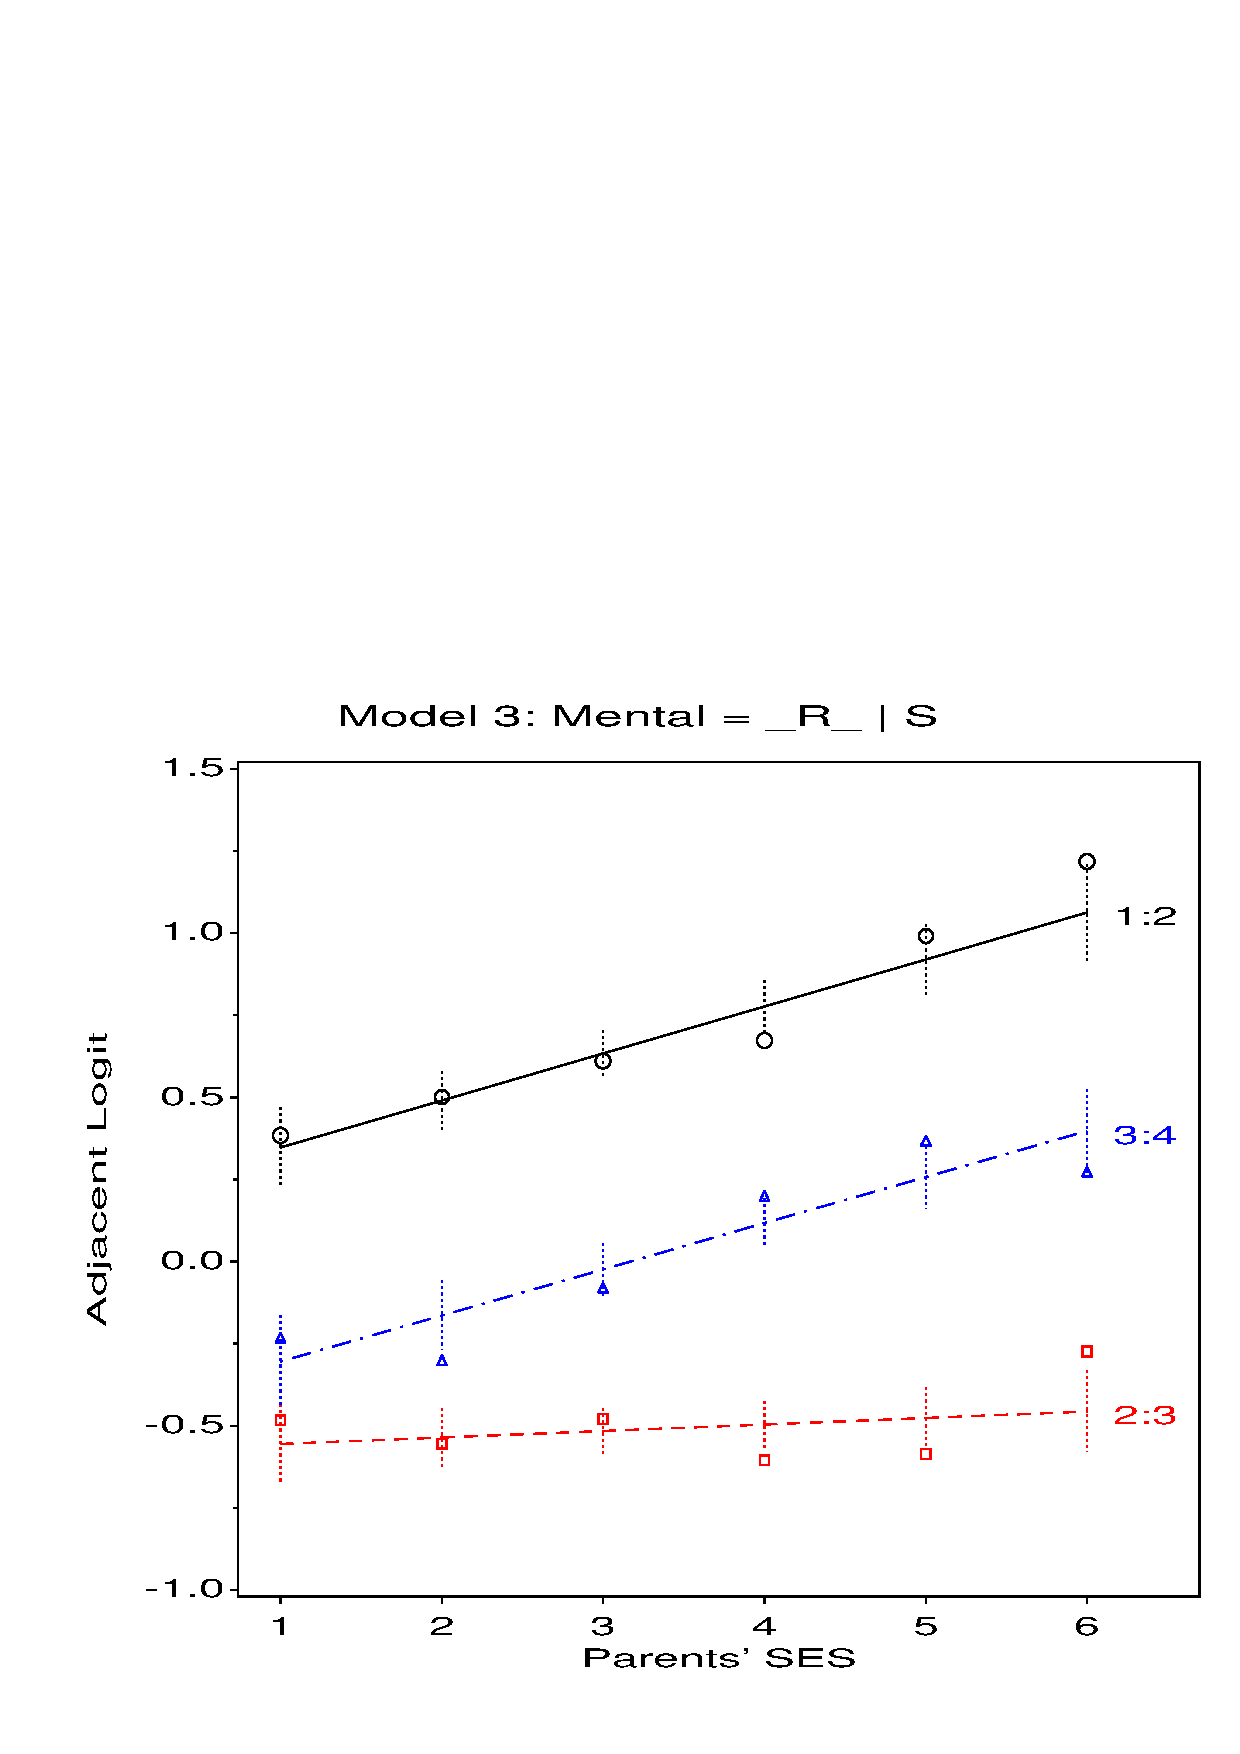
\includegraphics[width=1\linewidth]{mental43}
 \end{minipage}%
 \hfill
 \begin{minipage}[t]{.49\linewidth}
  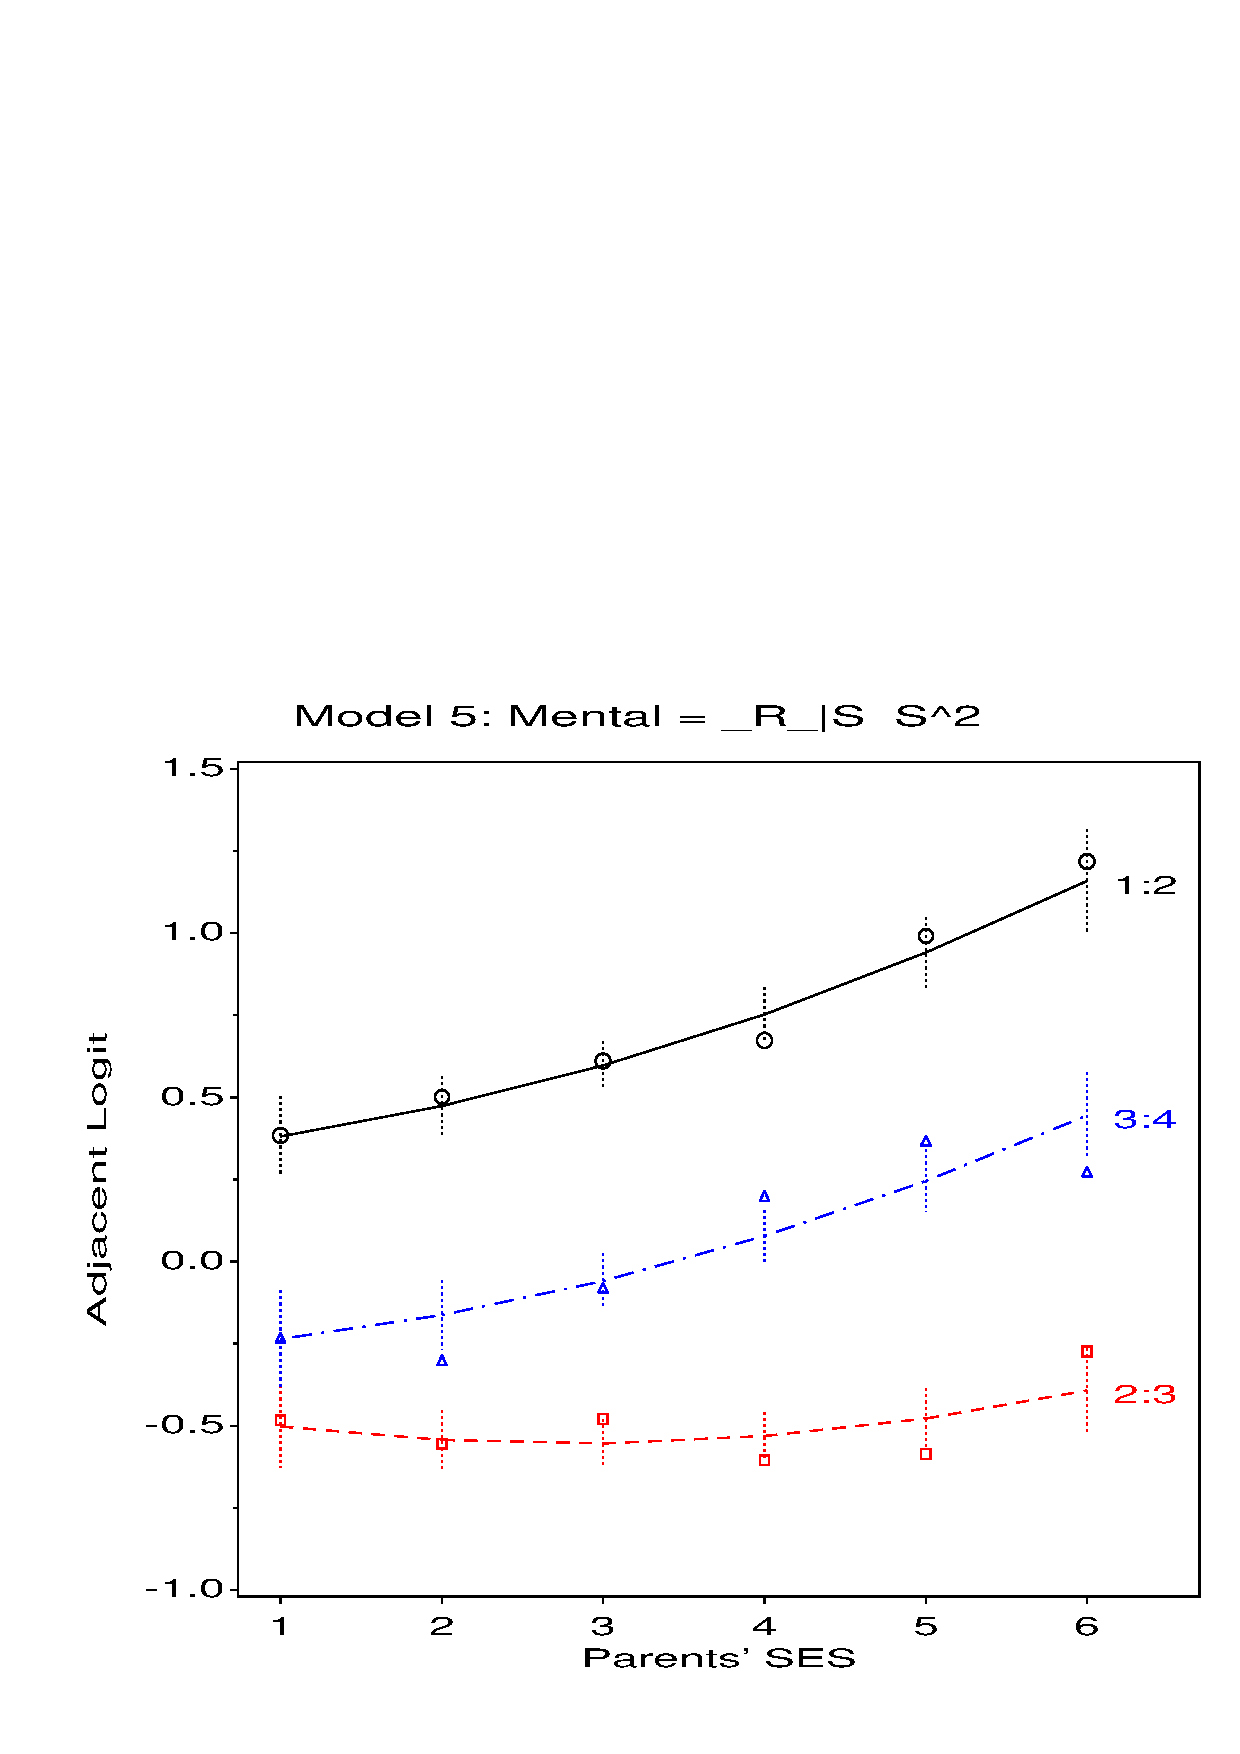
\includegraphics[width=1\linewidth]{mental44}
 \end{minipage}
 \caption{Adjacent category logit models for Mental Health data: Model 3 and Model 5}\label{fig:mental4b}
\end{figure}

What may we conclude from this?
From \tabref{tab:mentab4}, all models except the independence model
have acceptable fit according to the \chisq\ values;
Models 2--5 all have smaller AIC values than Model 1;  of these,
Model 2, the linear-by-linear is the most parsimonious, but Models
4 and 5 have slightly smaller AIC values.

One interpretation, from the plots in \figref{fig:mental4a} and \figref{fig:mental4b}
is that there is evidence that not both of SES and mental impairment
can be considered linear with unit spacing.
The intercepts suggest that the gap between categories 1 and 2
(`Well', 'Mild impairment') is greatest on the mental health scale,
and that between categories 2 and 3 (`Mild', `Moderate impairment')
is smallest.
The evidence regarding the metric for SES is more ambiguous:
there is a suggestion of a mildly quadratic relationship with SES,
particularly for the logit between response categories 1 and 2,
but this may be due to the points for (lowest) SES categories 5 and 6,
where the large logit values imply
a relatively larger number of people
classified as mildly impaired as opposed to well.
\end{Example}


\subsection{Cumulative logit models}\label{sec:loglin-ordcum}
When there is an ordinal response factor, cumulative logit models
\citep{WilliamsGrizzle:72} provide
an alternative way to take the ordinal nature of the response into account,
without assigning arbitrary scores to the response categories.

Let $F_j$ be the cumulative probability of a response less than or equal
to category $j$,
\begin{equation*}
F_j = \pi_1 + \pi_2 + \cdots + \pi_j  = \sum_{h=1}^{h=j} \pi_h
 \period
\end{equation*}
Then the \emph{cumulative logit} is defined as
\begin{equation*}%\label{eq:cumlogit}
C_j \equiv \logit ( 1 - F_j ) =
  \log \left( \frac { 1 - F_j }{F_j} \right) \period
\end{equation*}
$C_j$ gives the log odds that the response is in a category \emph{greater} than
category $j$, as opposed to a category less than or equal to $j$.
By this definition, the cumulative logits are necessarily
monotone decreasing over the response categories:
$C_1 \ge C_2 \ge \cdots \ge C_{J-1}$.
Models for the cumulative logit are particularly useful when the
response may be considered a discrete realization of an underlying
continuous variable.

In terms of cumulative logits, the model of independence is
\begin{equation*}%\label{eq:cindep}
C_{j|i} = \beta_j \comma
\end{equation*}
that is, the logit does not depend on explanatory variable(s) indexed
by subscript $i$.
Here, the response category parameters $\beta_j$ refer to the
cutpoints between adjacent categories, rather than to the distances
between adjacent ones as in the analogous adjacent category logit
model \eqref{eq:aindep}.

For quantitative scores, $a_i$, assigned to an explanatory variable,
the analog of the linear-by-linear model is
\begin{equation}\label{eq:clin}
 C_{j| i} = \beta_j + \gamma \: a_i
 \period
\end{equation}
which again has one more parameter than the independence model.
For any two rows, the difference in logits,
$C_{j| i} - C_{j| i'}$
is the log odds ratio in the $2\times 2$ table
for those two rows, with columns dichotomized following response category $j$.
Under model \eqref{eq:clin}, $C_{j| i} - C_{j| i'} = \gamma ( a_i - a_{i'})$,
so the log odds ratio is proportional to the difference in scale values,
and is the same at all cutpoints.
When unit-spaced scores, $\{a_i\} = i$ are used, the logit difference for
adjacent rows is then constant:
\begin{equation*}
 C_{j| i} - C_{j| i'} = \gamma
 \period
\end{equation*}

As with the adjacent category logits, a variety of models analogous to
the row effects model \eqref{eq:arow}, and
the linear-interaction model \eqref{eq:alin-int}
may be defined for the cumulative logits.
We illustrate these below, primarily to look at the shapes of plots
of observed and fitted logits, and to compare them with what we saw for
adjacent category logits.
\begin{Example}[mental3]{Mental impairment and parents' SES}
Cumulative logit models may be fit using \PROC{CATMOD} with the
\pname{RESPONSE CLOGIT;} statement.
The model is specified in the same way as for adjacent category
logits, but now the \verb|_RESPONSE_| keyword refers to
differences among the cumulative response probabilities.
As before,
an independent variable is treated as a quantitative variable,
when it is declared in a \stmt{DIRECT}{CATMOD}.

The following statements fit
the same models as in \exref{ex:mental4}: first Models 0--3
in which SES has no effect on mental health (Model 0), then SES with
a nominal effect (Model 1), a constant linear effect (Model 2)
and different linear effects for each cumulative logit (Model 3).
%% input: /users/faculty/friendly/sasuser/catdata/mental3.sas
%% last modified: 26-Nov-98 17:27
\begin{listing}
%include catdata(mental);

*-- Cumulative logit models;
proc catmod data=mental;
   weight count;
   population ses;
   response clogit / out=pred0;
   model mental = _response_ / noprofile noresponse title='Model 0: _R_';
  run;
   response clogit / out=pred1;
   model mental = _response_  ses / noprofile noresponse title='Model 1: _R_ SES';
  run;
   direct ses;
   response clogit / out=pred2;
   model mental = _response_  ses / noprofile noresponse title='Model 2:  _R_ S';
  run;
   direct ses;
   response clogit / out=pred3;
   model mental = _response_ | ses / noprofile noresponse title='Model 3:  _R_|S';
  run;
\end{listing}


For comparison, we also fit models with both linear and quadratic
effects on the cumulative logits,
first with equal slopes and curvature
for all response categories (Model 4), and second with separate slopes and
equal curvatures (Model 5).
%% input: /users/faculty/friendly/sasuser/catdata/mental3.sas
%% last modified: 29-Nov-98 11:55
\begin{listing}
data mental;
   set mental;
   ses2 = ses**2;

proc catmod data=mental;
   weight count;
   population ses;
   direct ses ses2;
   response clogit / out=pred4;
   model mental = _response_ ses ses2 / noprofile noiter title='Model 4: _R_ S S^2';
  run;
   response clogit / out=pred5;
   model mental = _response_|ses ses2 / noprofile noiter title='Model 5: _R_|S S^2';
  run;
\end{listing}


The model fit statistics for these models are shown in \tabref{tab:mentab3}.
The values are quite similar to those for the adjacent category logits
(\tabref{tab:mentab2}).
\begin{table}[htb]
 \caption{Cumulative logit models for Mental Health data}\label{tab:mentab3}
 \begin{center}
 \begin{tabular}{c l rrr r}
  \hline
  Model & Terms        & df & \chisq & $p$-value & AIC\\ 
  \hline
  0 & \verb\_R_\       & 15 & 45.92 & 0.0001 &  15.92\\ 
  1 & \verb\_R_| SES\  & 10 &  7.75 & 0.6536 & -12.25\\ 
  2 & \verb\_R_ S\     & 14 & 10.72 & 0.7080 & -17.28\\ 
  3 & \verb\_R_|S\     & 12 &  6.48 & 0.8897 & -17.52\\ 
  4 & \verb\_R_ S S^2\ & 13 &  8.36 & 0.8192 & -17.64\\ 
  5 & \verb\_R_|S S^2\ & 11 &  3.94 & 0.9716 & -18.06\\ 
  \hline
 \end{tabular}
 \end{center}
\end{table}


For any such model, the \macro{CATPLOT} displays the observed and fitted
cumulative logits using the \ODS\ specified on the
\stmt{RESPONSE}{CATMOD}.
The statements below produce the graphs of the logits for Model 0,
and Model 1,
shown in \figref{fig:mental3a}.
Similar statements, using the \ODS s \pname{PRED2} and \pname{PRED4},
give the graphs for Model 2 and Model 4 in \figref{fig:mental3b}.
%% input: /users/faculty/friendly/sasuser/catdata/mental3.sas
%% last modified: 02-Dec-98 15:47
\begin{listing}
axis1 label=(a=90);
axis2 offset=(3,6);
proc format;
   value cum 1='>1'  2='>2'  3='>3';
title 'Model 0: Mental = _R_';
%catplot(data=pred0, x=ses, y=_obs_, class=_number_, clfmt=cum.,
   type=FUNCTION, ylab=Cumulative Logit);
title 'Model 1: Mental = _R_ SES';
%catplot(data=pred1, x=ses, y=_obs_, class=_number_, clfmt=cum.,
   type=FUNCTION, ylab=Cumulative Logit);
\end{listing}


%% two subfig side-by-side
\begin{figure}[htb]
 \begin{minipage}[t]{.49\linewidth}
  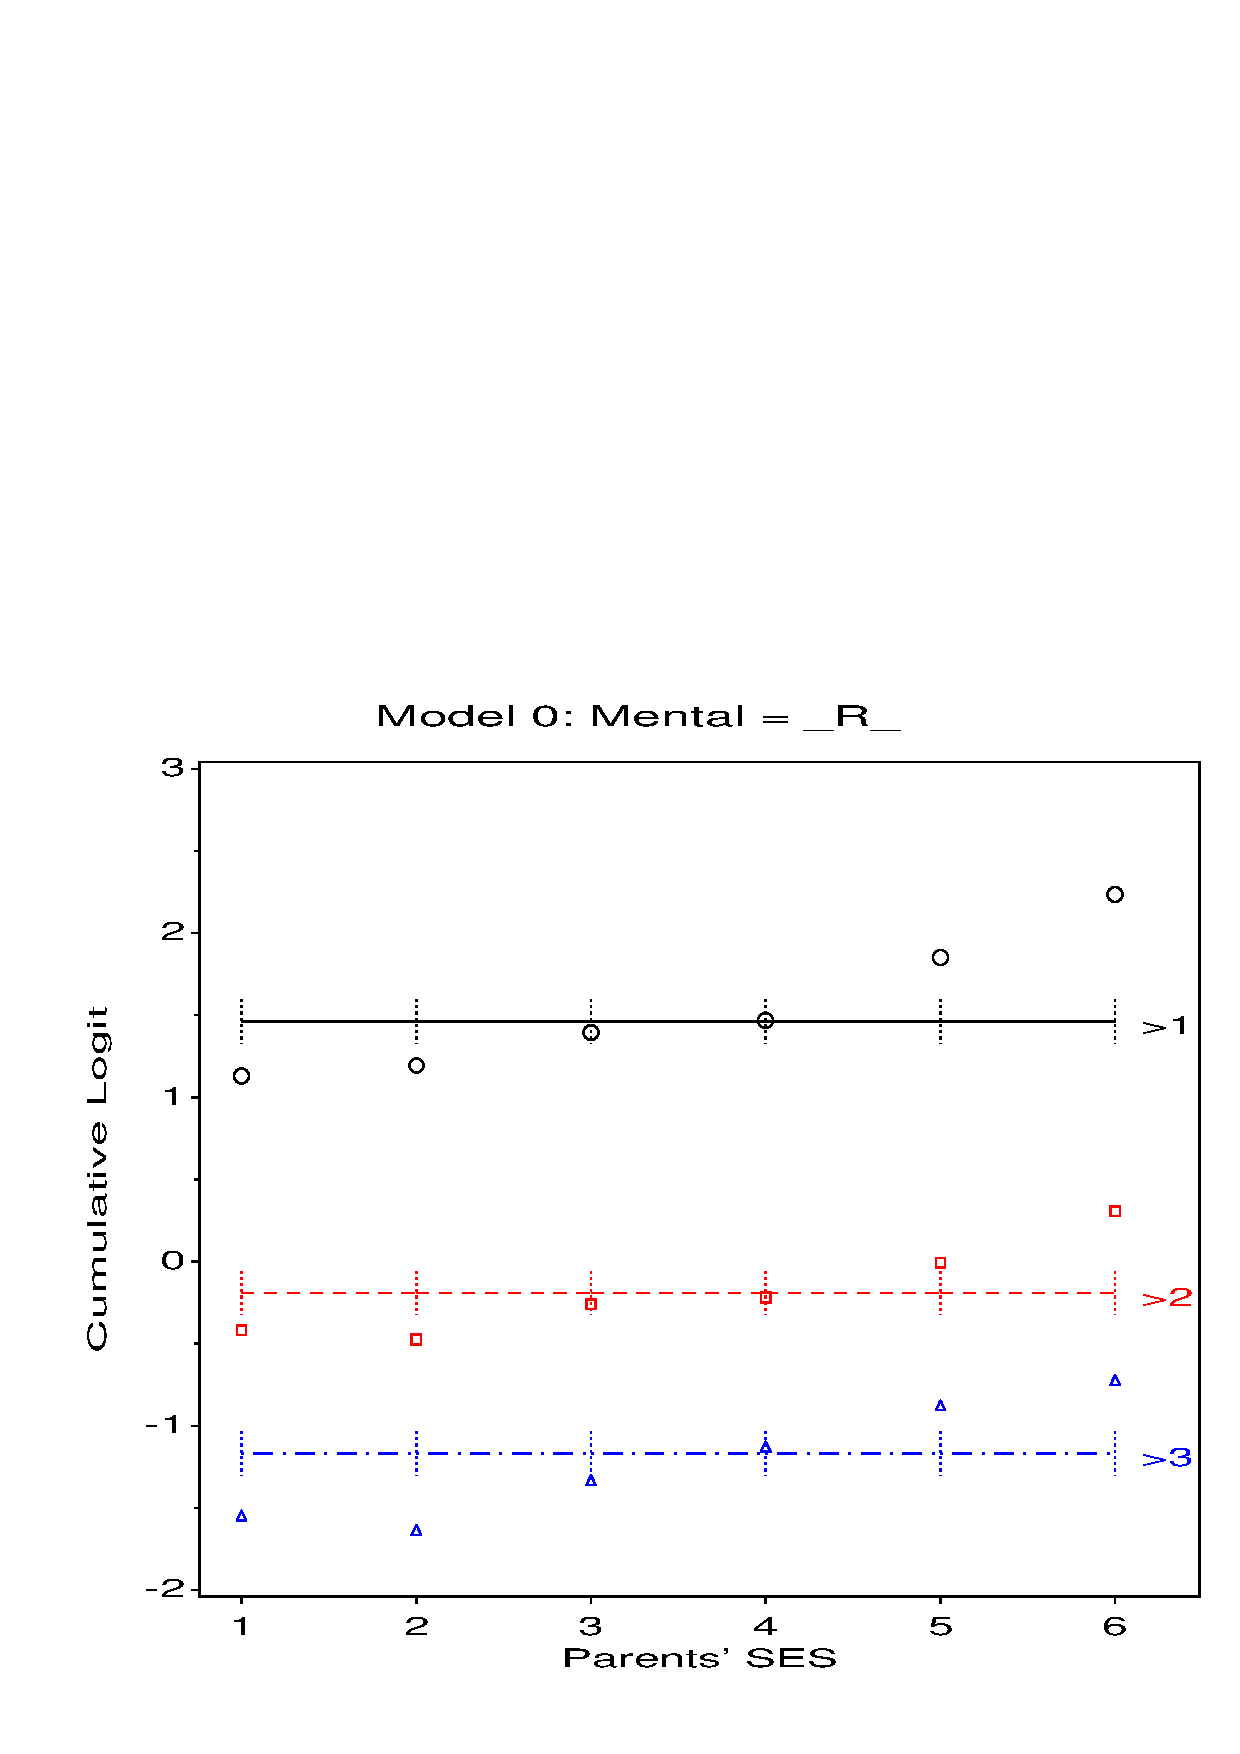
\includegraphics[width=1\linewidth]{mental31}
 \end{minipage}%
 \hfill
 \begin{minipage}[t]{.49\linewidth}
  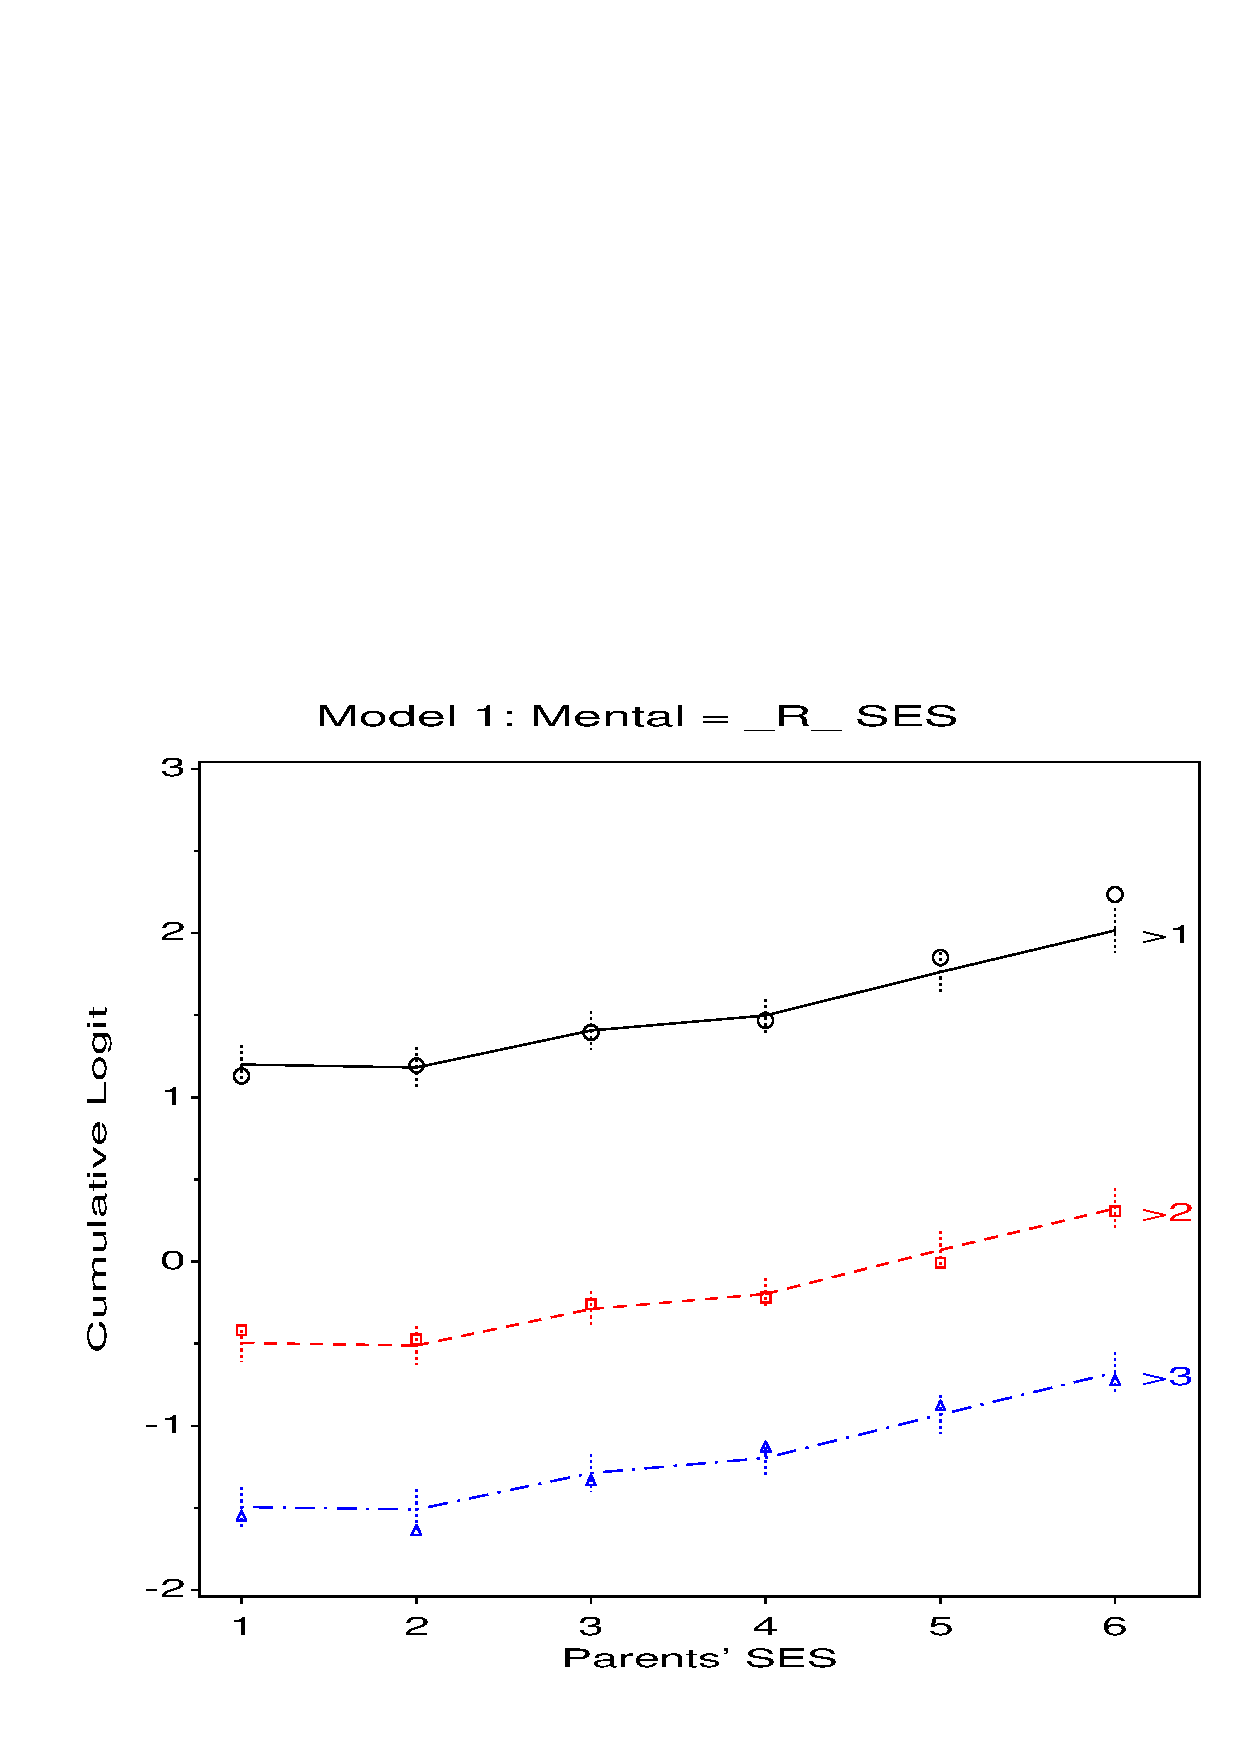
\includegraphics[width=1\linewidth]{mental32}
 \end{minipage}
 \caption{Cumulative logit models for Mental Health data, Model 0 and Model 1}\label{fig:mental3a}
\end{figure}

%% two subfig side-by-side
\begin{figure}[htb]
 \begin{minipage}[t]{.49\linewidth}
  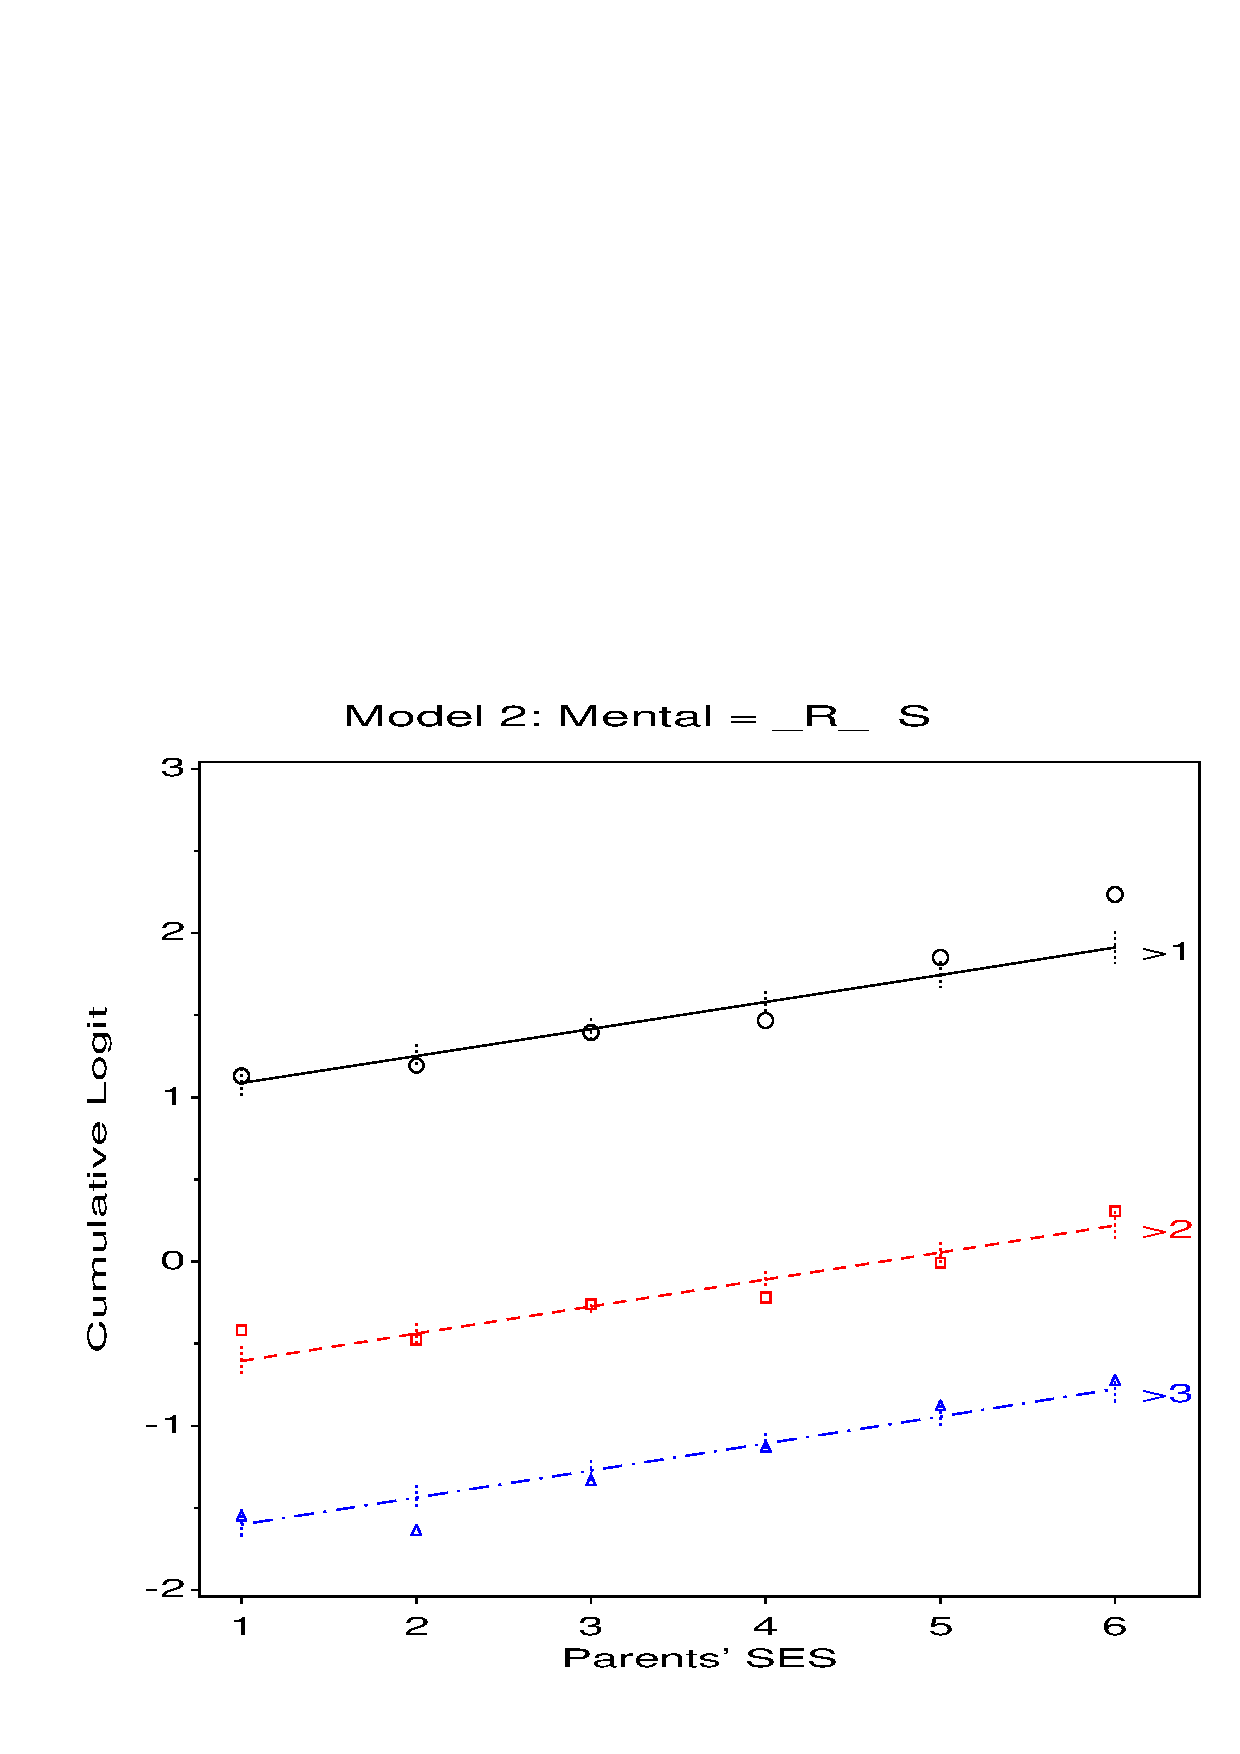
\includegraphics[width=1\linewidth]{mental33}
 \end{minipage}%
 \hfill
 \begin{minipage}[t]{.49\linewidth}
  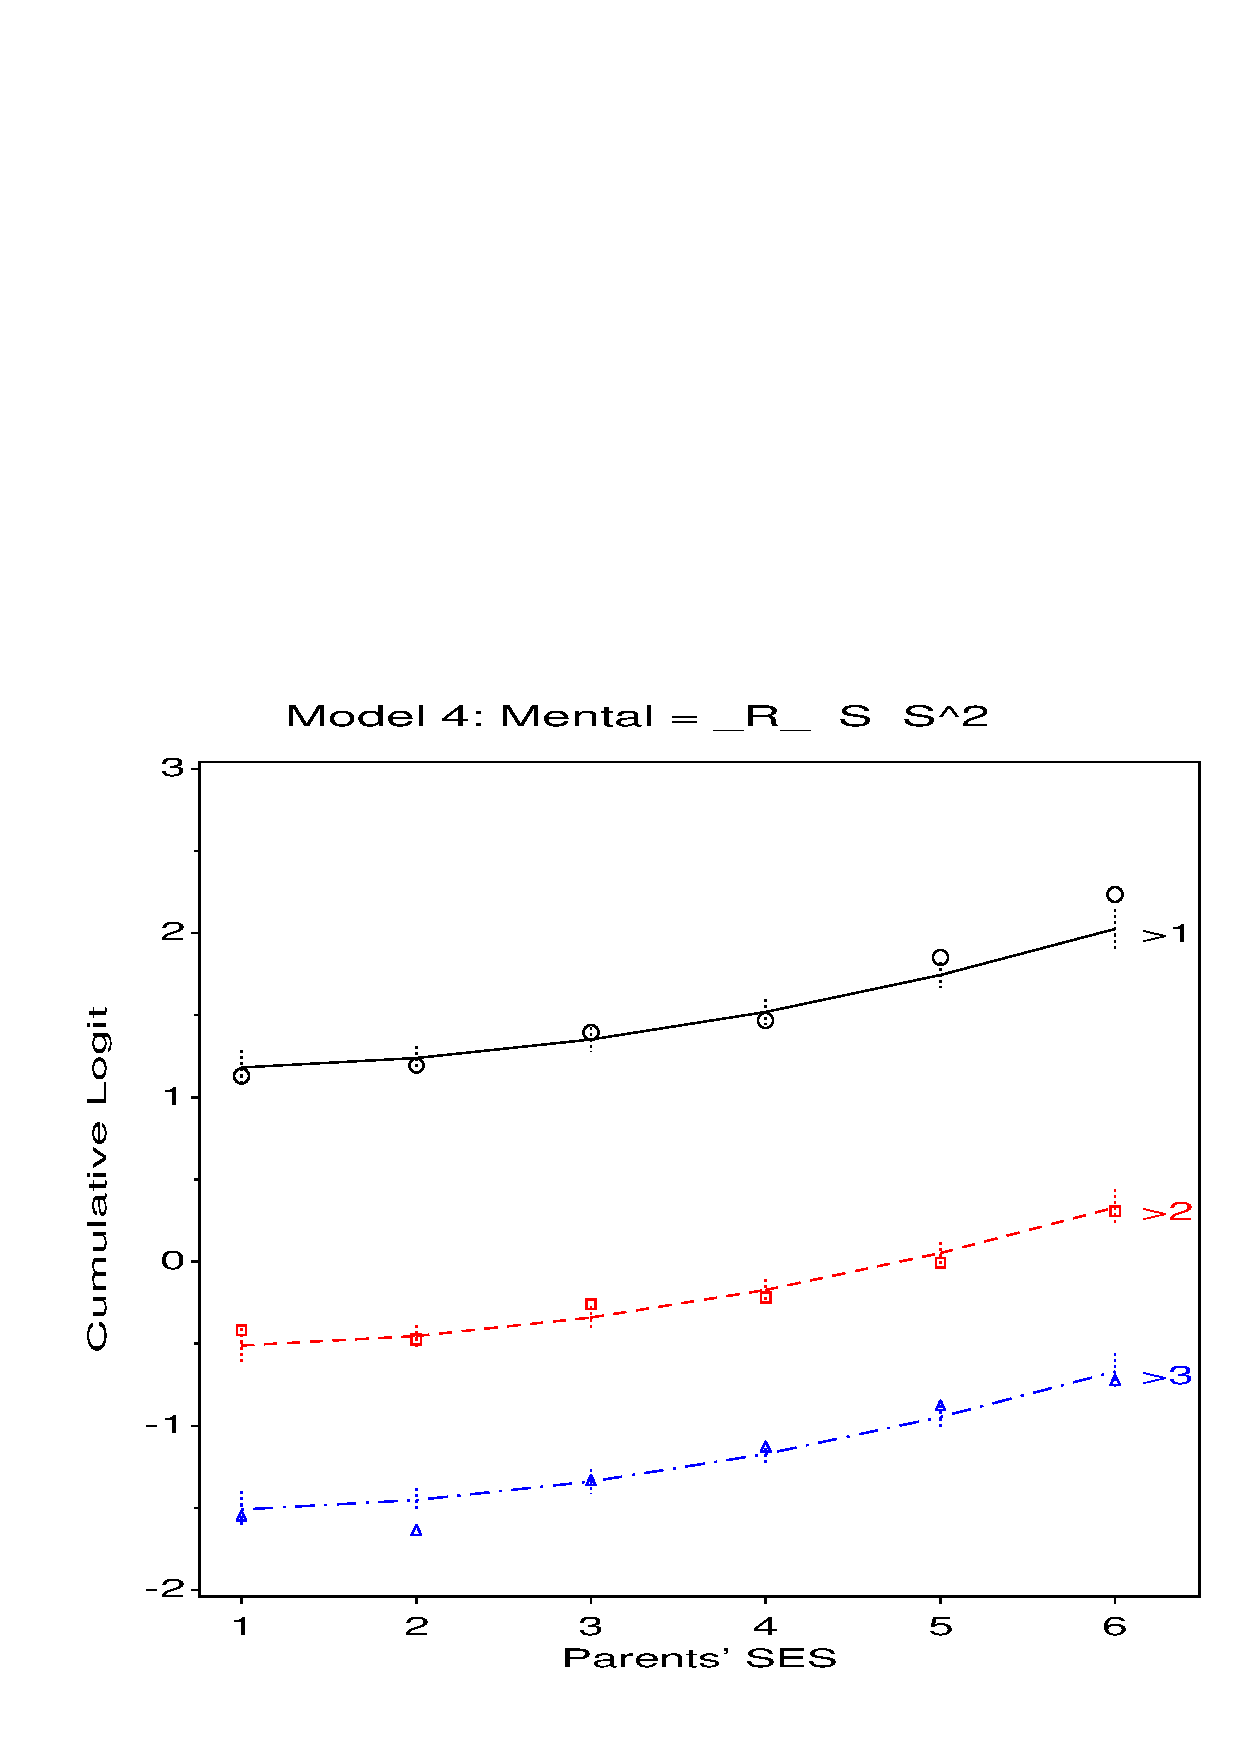
\includegraphics[width=1\linewidth]{mental35}
 \end{minipage}
 \caption{Cumulative logit models for Mental Health data: Model 2 and Model 4}\label{fig:mental3b}
\end{figure}
\end{Example}


\section{An extended example}\label{sec:loglin-vietnam}
Any model is a summary, and even a reasonably good-fitting model is not always sensible or faithful to the details of the data.
The interplay between graphing and fitting is important in arriving at
an understanding of the relations among the variables
and an adequate descriptive model.
This section describes the analysis of a moderately large three-way
table, where we find that graphical displays play a crucial role
in directing our understanding and model representation.

\begin{Example}[vietnam1]{Student opinion about the Vietnam war}
In May 1967 a survey of student opinion on U.S. policies toward the war in Vietnam was undertaken at the University of North Carolina at Chapel Hill.
Students were asked which of four policies they supported.  The alternatives stated that the US should \dots:
\begin{description*}
\item[A] defeat North Vietnam by widespread bombing and by land invasion.
\item[B] follow the present policy.
\item[C] de-escalate military activity, stop bombing, and intensify efforts to begin negotiations.
\item[D] withdraw military forces immediately.
\end{description*}
The responses were classified by gender and by student status (undergraduate year, or graduate student),  published in the student newspaper, and subsequently analyzed by \citet{Aitkin-etal:89}.  The data are shown in
\tabref{tab:vietnam1} and listed in the \Dset\ \pname{VIETNAM}
in \datref{dat:vietnam}.
\begin{table}[htb]
 \caption{Student opionion on Vietnam war policy}\label{tab:vietnam1}
 \begin{center}
 \begin{tabular}{ll rrrr rrr}
  \hline
       &       &  \multicolumn{4}{c}{Response} \\ \cline{3-6}
Sex    & Year  &   A  &  B  &  C  &  D  & Total & Enroll & \% Resp \\ \hline
Male   & 1     &  175 & 116 & 131 &  17 & 439 & 1768 & 24.8 \\ 
       & 2     &  160 & 126 & 135 &  21 & 442 & 1792 & 24.7 \\ 
       & 3     &  132 & 120 & 154 &  29 & 435 & 1693 & 25.7 \\ 
       & 4     &  145 &  95 & 185 &  44 & 469 & 1522 & 30.8 \\ 
       & Grad  &  118 & 176 & 345 & 141 & 780 & 3005 & 26.0 \\[.5ex] 
Female & 1     &   13 &  19 &  40 &   5 &  77 &  487 & 15.8 \\ 
       & 2     &    5 &   9 &  33 &   3 &  50 &  326 & 15.3 \\ 
       & 3     &   22 &  29 & 110 &   6 & 167 &  772 & 21.6 \\ 
       & 4     &   12 &  21 &  58 &  10 & 101 &  608 & 16.6 \\ 
       & Grad  &   19 &  27 & 128 &  13 & 187 & 1221 & 15.3 \\ 
  \hline
 \end{tabular}
 \end{center}
\end{table}


The survey was not designed to yield a representative sample
(survey ballots were merely made available in the student council building)
and the response rates, shown in \tabref{tab:vietnam1}, were low overall
and varied somewhat according to year and gender.
We cannot, therefore, draw conclusions about the attitudes of the whole student population.
However, we can study how the preferred policy varies with sex and year of study, among those who responded.
This means that the total numbers of each sex and year should be regarded
as fixed, and the [SexYear] term must be included in any model.
Note that both the response and year might reasonably be treated as ordinal
variables.

The \Dset\ \pname{vietnam}, listed in \datref{dat:vietnam}, is created in frequency form
with the variables \pname{sex}, \pname{year}, \pname{response}, and
\pname{count}.  Both \pname{year} and \pname{response} are created as
numeric variables to allow them to be treated as ordinal (or interval)
variables, and formats are created to associate descriptive labels
as needed.

Because response choice is the natural outcome variable, it is useful
to begin with a simple graph showing the proportions of choices
for each Sex-Year group, shown in \figref{fig:vietprob}.
%% two subfig side-by-side
\begin{figure}[htb]
 \begin{minipage}[t]{.49\linewidth}
  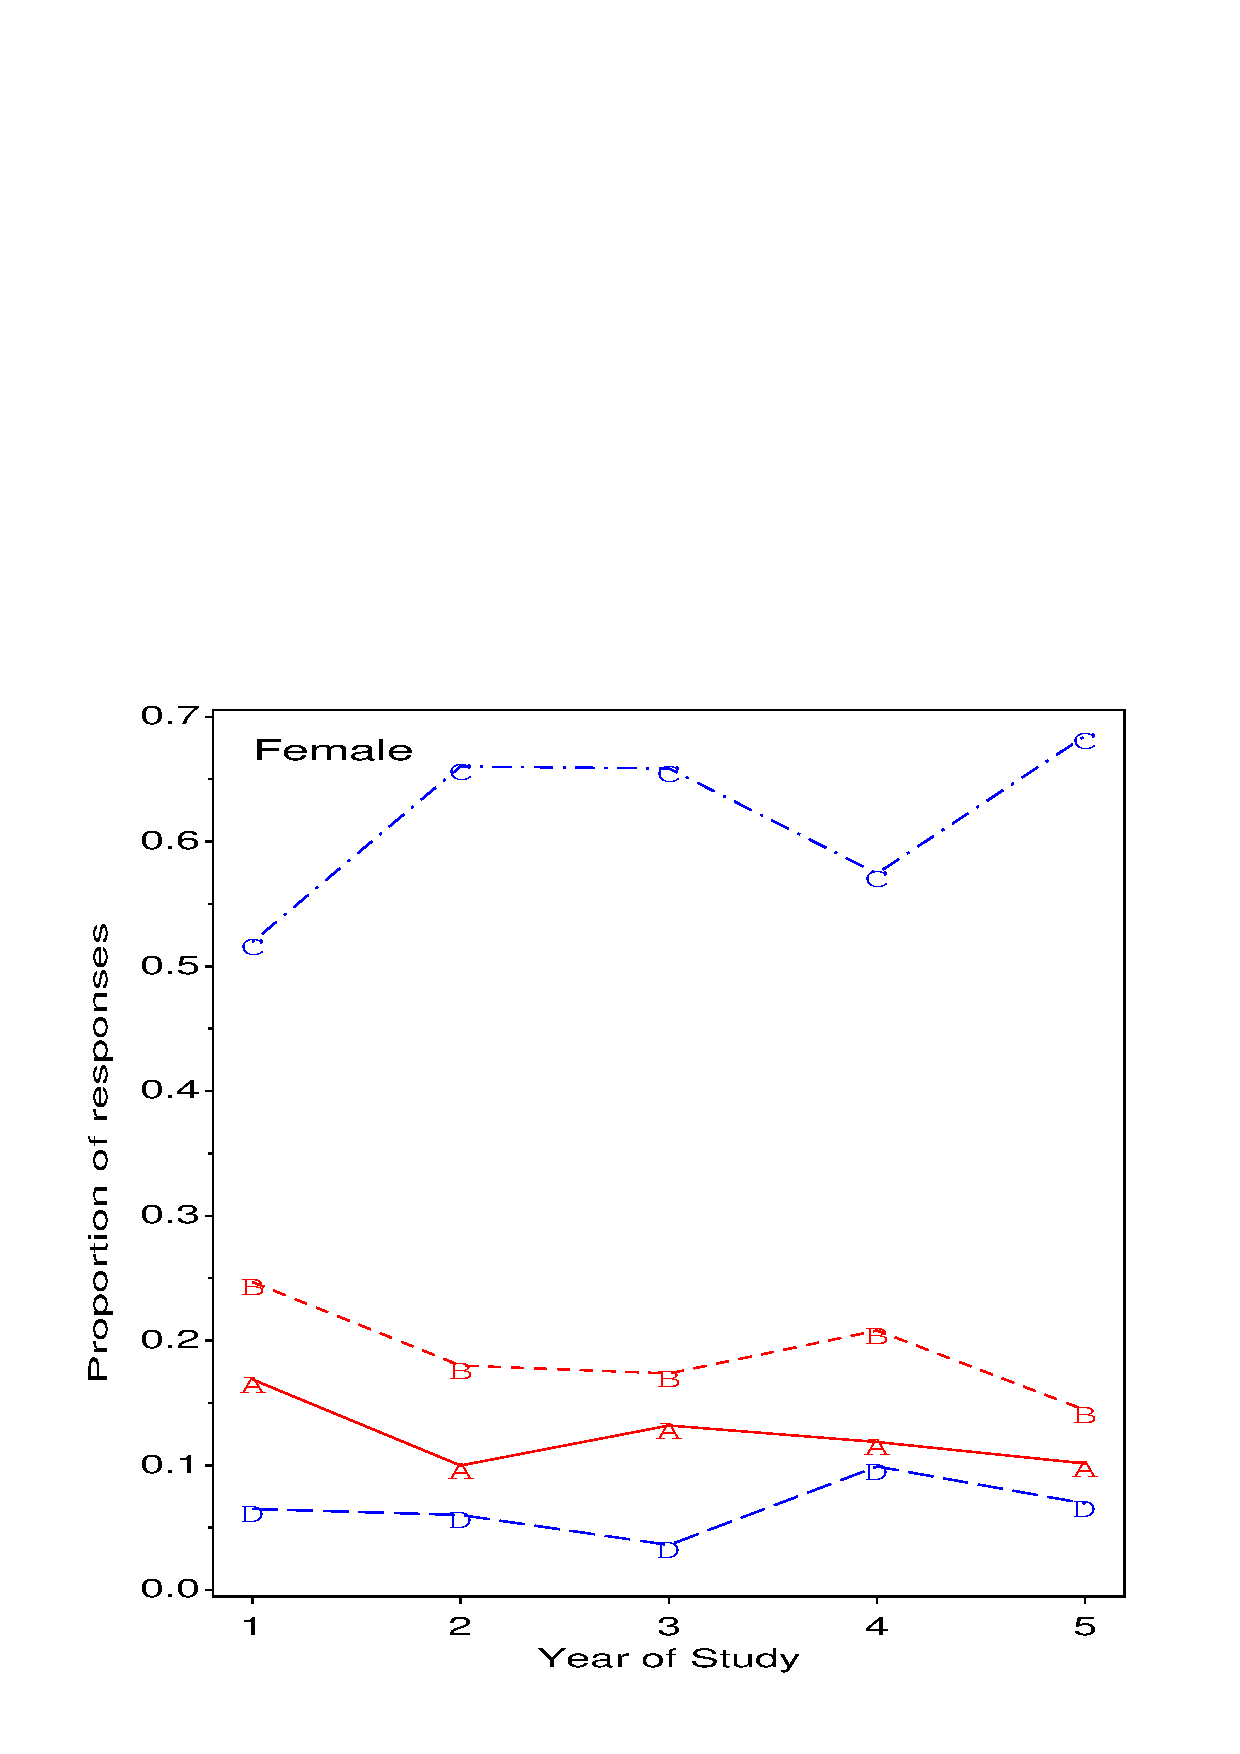
\includegraphics[width=1\linewidth]{vietprob1}
 \end{minipage}%
 \hfill
 \begin{minipage}[t]{.49\linewidth}
  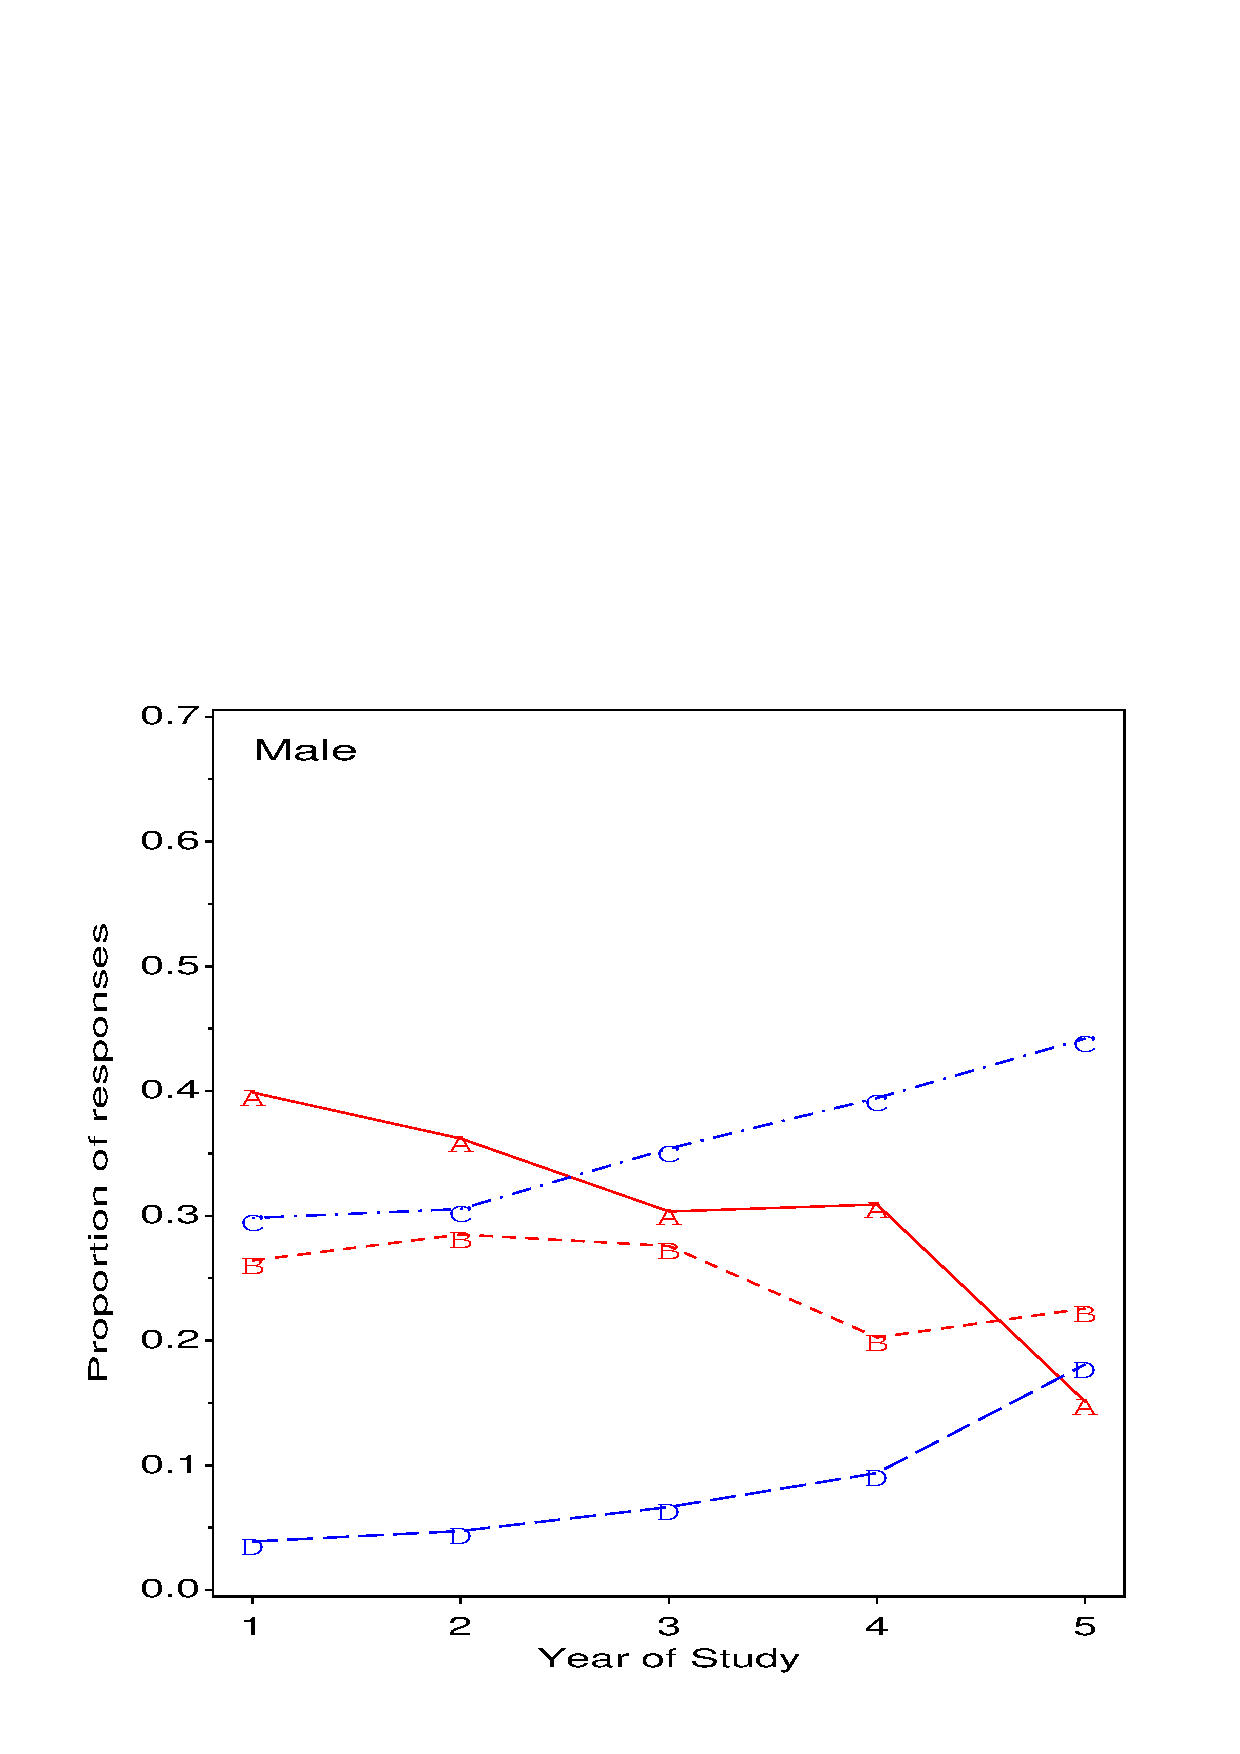
\includegraphics[width=1\linewidth]{vietprob2}
 \end{minipage}
 \caption[Response probabilities for Vietnam data]{Response probabilities for Vietnam data.  Point labels indicate the response category.}\label{fig:vietprob}
\end{figure}
To do this, we find the total number of respondents in each group,
merge this with the data, and calculate the proportions.
%% input: /users/faculty/friendly/sasuser/catdata/vietprob.sas
%% last modified: 23-Oct-98  9:38
\begin{listing}
%include catdata(vietnam);

*-- Get row totals for sex-year;
proc summary data=vietnam nway;
   class sex year;
   var count;
   output out=totals sum=total;

*-- Merge, compute proportions;
data vietnam;
   merge vietnam totals(keep=sex year total);
   by sex year;
   p = count / total;
   label p='Proportion of responses';
\end{listing}

Then, we can plot \pname{p} against \pname{year} for each \pname{sex},
giving the graphs shown in \figref{fig:vietprob}:
%% input: /users/faculty/friendly/sasuser/catdata/vietprob.sas
%% last modified: 23-Oct-98  9:38
\begin{listing}
goptions hby=0;
proc gplot data=vietnam;
   plot p * year = response / 
      frame vaxis=axis1 haxis=axis2 hm=0 vm=1 nolegend anno=label;
   by sex;
   symbol1 v=A h=2 i=join c=red  l=1;
   symbol2 v=B h=2 i=join c=red  l=20;
   symbol3 v=C h=2 i=join c=blue l=41;
   symbol4 v=D h=2 i=join c=blue l=21;
   axis1 label=(a=90) order=(0 to .7 by .1);
   axis2 offset=(3);
\end{listing}


From these graphs, we see that women choose response C, ``begin negotiations''
most often, and the ranking of their choices is relatively
constant over years.
For men, however, the proportions choosing ``doveish'' responses C and D increase
consistently over years, while the proportions for A and B decrease.
We keep these observations in mind as we begin to search for a descriptive model.

We begin by fitting the baseline ``null'' model, $[SY][R]$, which includes the
$[SY]$ association, but no association between response and sex or year.
This model implies that the response curves in \figref{fig:vietprob}
should all be flat (no year effect) and at the same levels in the two
panels (no sex effect).
The model fit is very poor ($G^2$ (27) = 361.72), and the patterns in
\figref{fig:vietprob} lead us to add sex and year effects, giving
the model $[SY][RS][RY]$.
These two models are fit using \PROC{CATMOD} using the
\stmt{LOGLIN}{CATMOD} as follows:
%% input: /users/faculty/friendly/sasuser/catdata/vietnam1.sas
%% last modified: 23-Oct-98  9:59
\begin{listing}
*-- Fit as loglin models;
proc catmod data=vietnam;
   weight count;
   model response * sex * year = _response_ /
         ml noiter noresponse nodesign nogls noprofile;
   loglin response sex|year / title='Null model';
 run;
   loglin sex|year response|sex response|year / title='Sex+Year';
 run;
\end{listing}


The model summary statistics from this step are shown in
\outref{out:vietnam1.1}.  For the second model, the
$[RS]$ and $[RY]$ terms are both large, and the model
fit is dramatically improved.
Given the large sample size, we might accept this as
an adequate model, particularly if we had not plotted the data.

\begin{Output}[htb]
\caption{Model fit summaries for initial models, Vietnam war data}\label{out:vietnam1.1}
\small
\verbatiminput{ch7/out/vietnam1.1}
\end{Output}

%% two subfig side-by-side
\begin{figure}[htb]
 \begin{minipage}[t]{.49\linewidth}
  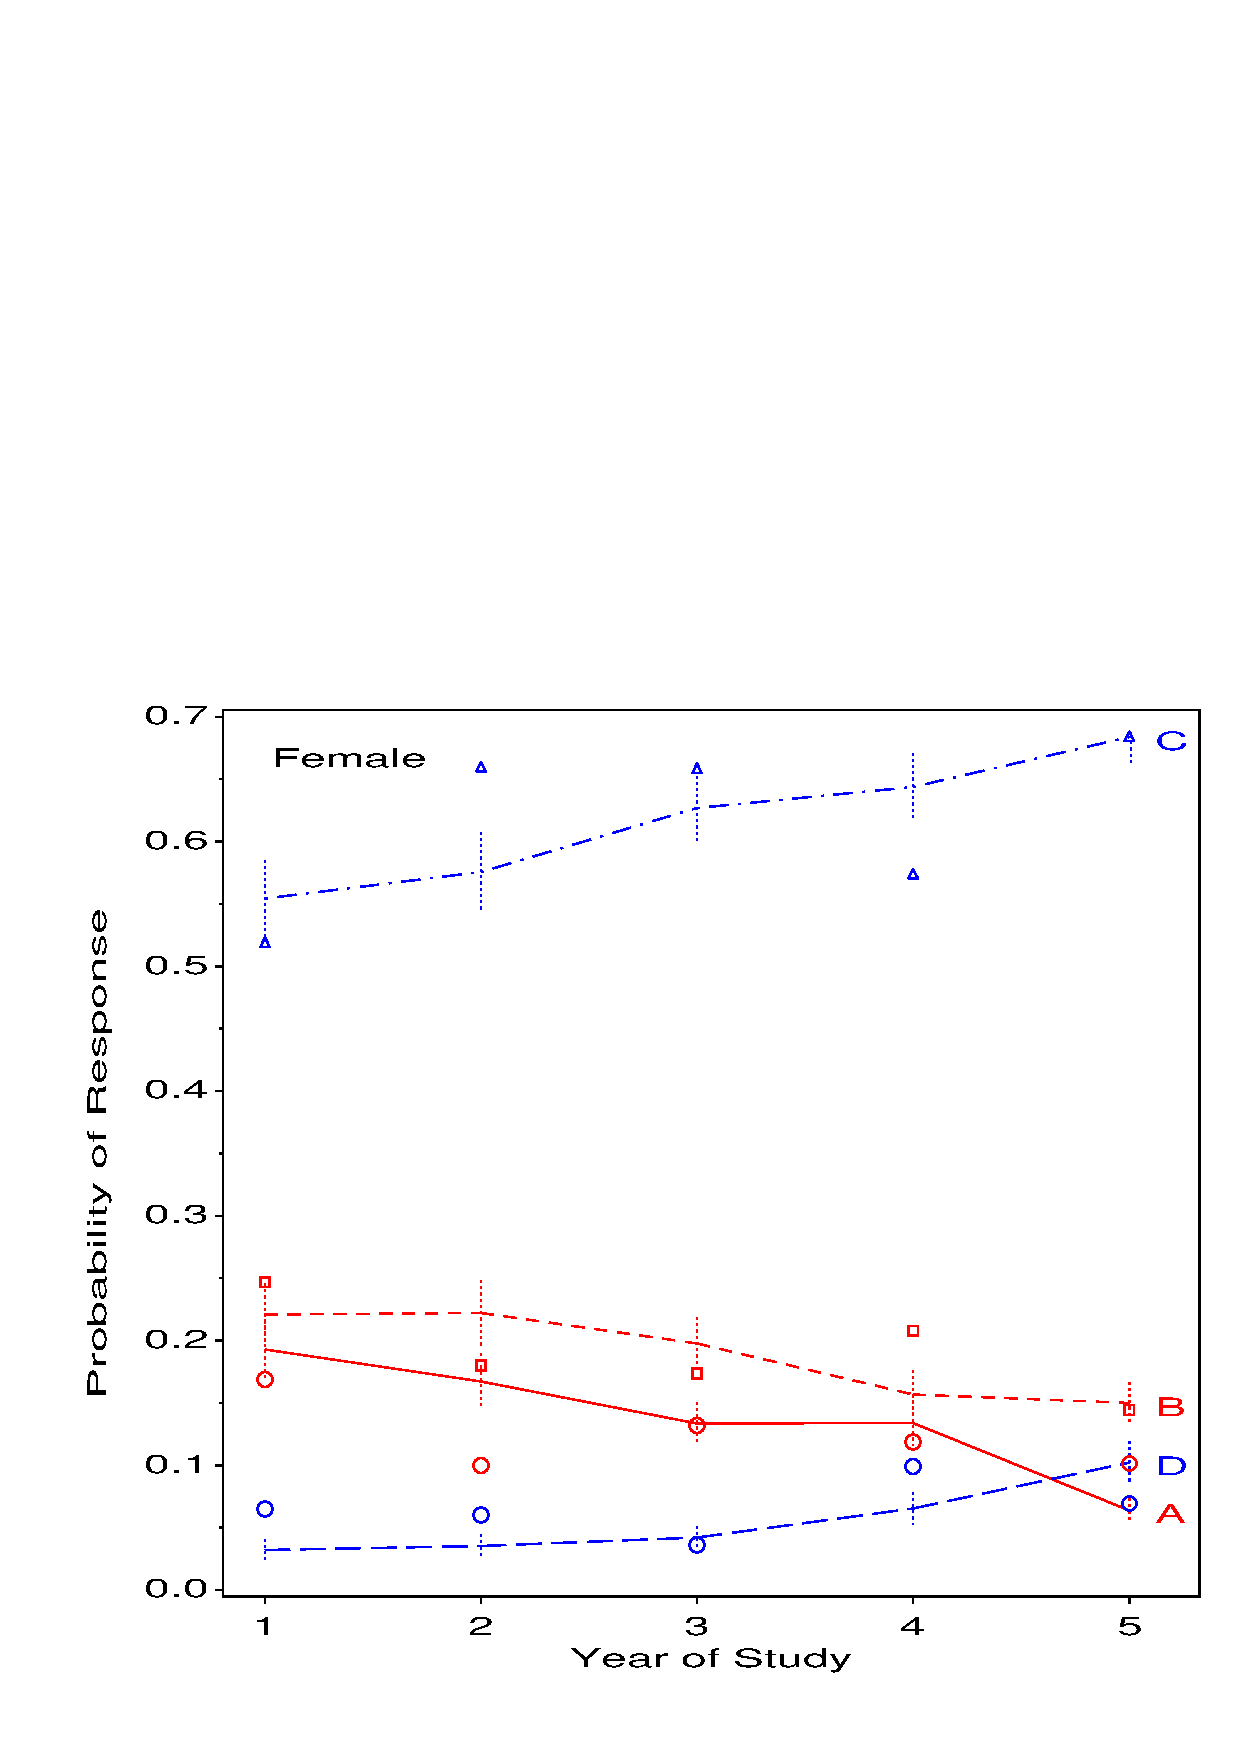
\includegraphics[width=1\linewidth]{vietnam11}
 \end{minipage}%
 \hfill
 \begin{minipage}[t]{.49\linewidth}
  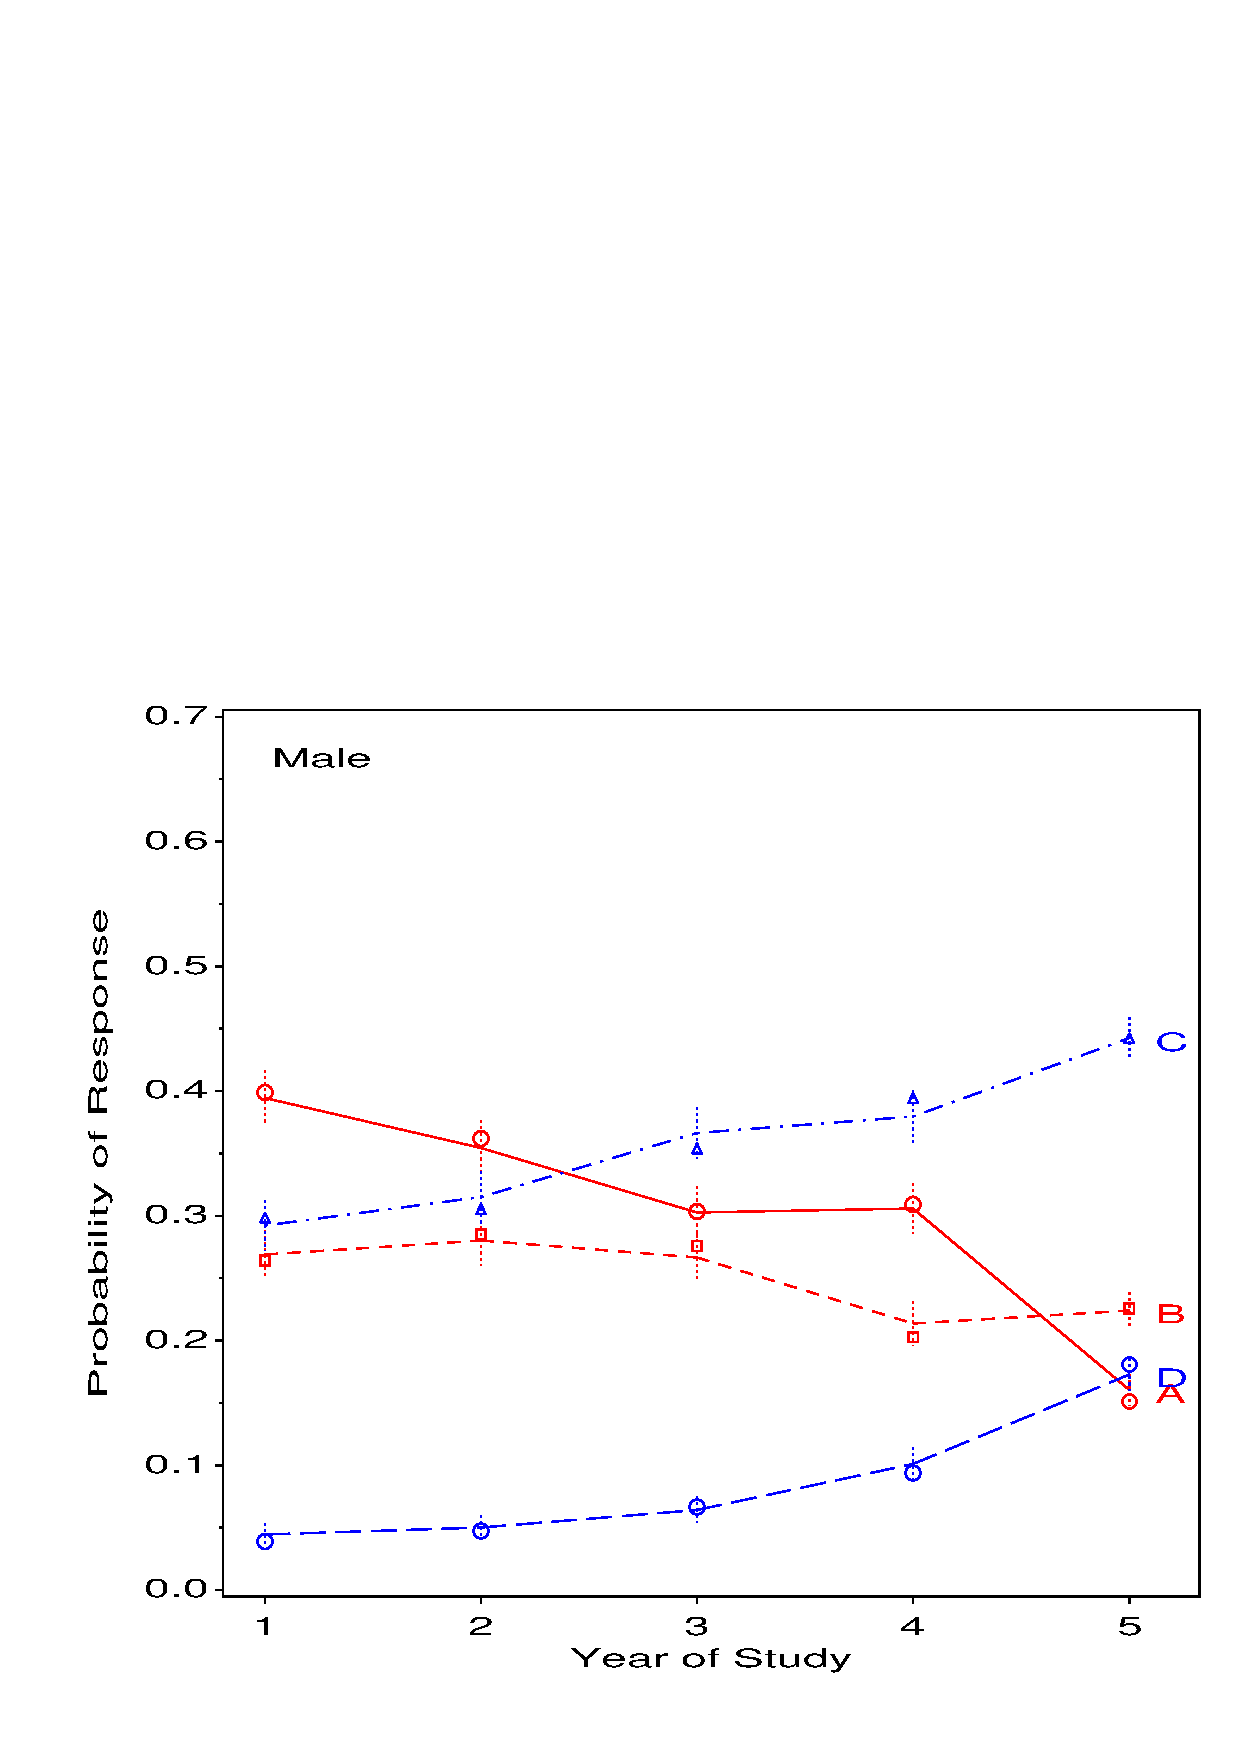
\includegraphics[width=1\linewidth]{vietnam12}
 \end{minipage}
 \caption{Observed and fitted probabilities for model $[SY][RS][RY]$}\label{fig:vietnam1}
\end{figure}

The \LR\ \GSQ\ for the Sex+Year model, 19.19 on 12 df, corresponds to the three-way
term, $[RSY]$.  Excluding it from the model means that the
relationship between response and year is the same for men and
women, yet we have seen in \figref{fig:vietprob} that this
is unlikely to be true.  There is something wrong with the Sex+Year
model.

We can confirm these suspicions by plotting predicted probabilities
under the model together with the observed response probabilities.
For a \loglin\ model,
\PROC{CATMOD} gives fitted \emph{frequencies}, and we could divide these
by the totals as we did to produce \figref{fig:vietprob}.
It is somewhat easier to fit the equivalent logit model for \pname{response},
for which the fitted values (with \verb|_TYPE_='PROB'| in the \ODS) are probabilities.
The \macro{CATPLOT} produces \figref{fig:vietnam1}.
%% input: /users/faculty/friendly/sasuser/catdata/vietnam1.sas
%% last modified: 23-Oct-98  9:59
\begin{listing}
*-- Fit as logit models;
proc catmod data=vietnam;
   weight count;
   population sex year;
   response logit;
   model response = / ml noiter noprofile title='Null model';
 run;
   response logit / out=fit;
   model response = sex year/ ml noiter noprofile title='Sex+Year';
 run;

axis1 label=(a=90) order=(0 to .7 by .1);
axis2 offset=(3,5);
%catplot(data=fit,
   x=year, y=_obs_,
   type=PROB,
   class=response, clfmt=letter.,
   byvar=sex, byfmt=$sex.,
   vaxis=axis1, haxis=axis2,
   colors=red red blue blue,
   ylab=Probability of Response);
\end{listing}


The fitted probabilities are reasonably close for males, but quite poor for females.  Perhaps we need to fit different models for men and women.
The saturated \loglin\ model, $[RSY]$ corresponds to the logit model
$R = S | Y = S + Y + S*Y$.
We can examine the possibility of different year effects for men and women within the logit formulation by nesting the effect of year within sex.
(This is equivalent to fitting separate models, $R = Y$, by sex.)
%% input: /users/faculty/friendly/sasuser/catdata/vietnam1.sas
%% last modified: 20-Nov-98  9:49
\begin{listing}
*-- Year within Sex;
proc catmod data=vietnam;
   weight count;
   population sex year;
   model response = sex  year(sex='F')  year(sex='M')
     / ml noiter noprofile title='Year within Sex';
   response logit ;
\end{listing}


The output, shown in \outref{out:vietnam1.2}, indicates that the year
effect for women is quite small ($\GSQ(12) = 12.96$) and can be dropped
from the model.
Removing the term \pname{year(sex='F')} from the \pname{model} statement
gives an adequate model;
the residual $\GSQ(12) = 12.96$ in the revised model
is (coincidently) just that for the term dropped.
\begin{Output}[htb]
\caption{Vietnam war data, Nested year effect model}\label{out:vietnam1.2}
\small
\verbatiminput{ch7/out/vietnam1.2}
\end{Output}

We noticed earlier that the response probabilities for men were consistently
increasing or decreasing with year.  Perhaps we can simplify the model
by using year as a linear effect.  To do this, we just add the statement
\pname{DIRECT YEAR;}.
%% input: /users/faculty/friendly/sasuser/catdata/vietnam2.sas
%% last modified: 20-Nov-98 11:05
\begin{listing}
*-- Year-linear within Males;
proc catmod data=vietnam;
   weight count;
   population sex year;
   direct year;
   model response = sex year(sex='M')
       / ml noiter noprofile title='Year-linear within Males';
   response / out=fit;
\end{listing}


The model fit statistics for this model (\outref{out:vietnam2.1})
suggests there is some lack-of-fit, however, with $\GSQ (21) = 38.10$.
To see why, plot the observed and fitted probabilities again.
Because the plot is determined completely by the \ODS\ \pname{fit},
we use exactly the same \pname{\%catplot} call as for \figref{fig:vietnam1}.
The result is shown in \figref{fig:vietnam2}.
\begin{Output}[htb]
\caption{Vietnam war data, Linear year effect for males}\label{out:vietnam2.1}
\small
\verbatiminput{ch7/out/vietnam2.1}
\end{Output}

Most of the observed points in \figref{fig:vietnam2} are quite close to
the fitted values (the error bars show $\pm 1$ standard error
around the predicted probability). However, there are a few scattered points for
females and a couple for males (4th year, responses A and B) which appear poorly fit.

We should certainly examine residuals more closely
to see if the lack-of-fit is localized to these few cells
or whether there is a more general way to improve the model.
For example,  the two points for 4th year men
indicate a tendency for them to select response B less than the model predicts, and to select
response A more often.
 \citet{Aitkin-etal:89} make the reasonable
suggestion that these draft-eligible men would eschew the ``present policy''
under which their chances of being drafted would increase.
But perhaps it's time to look at these data from another perspective.

%% two subfig side-by-side
\begin{figure}[htb]
 \begin{minipage}[t]{.49\linewidth}
  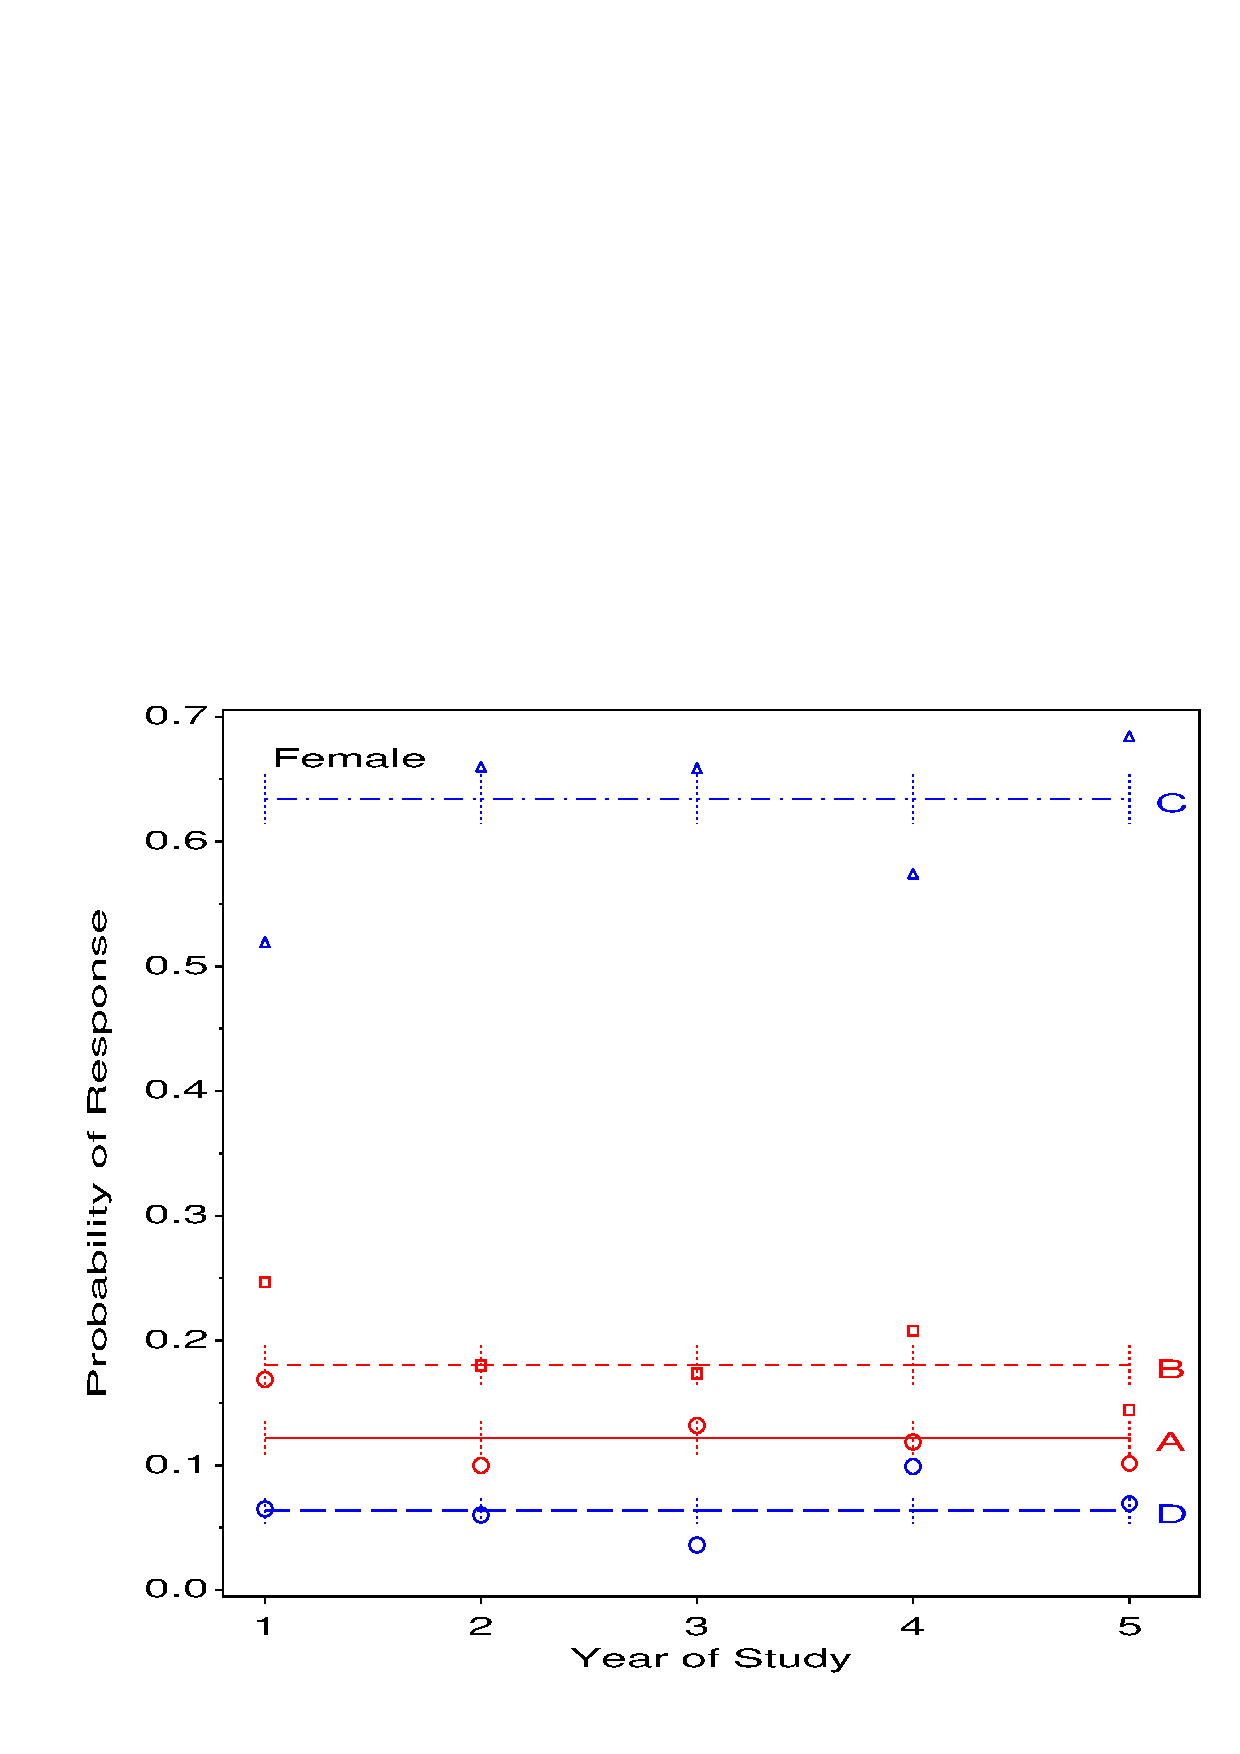
\includegraphics[width=1\linewidth]{vietnam21}
 \end{minipage}%
 \hfill
 \begin{minipage}[t]{.49\linewidth}
  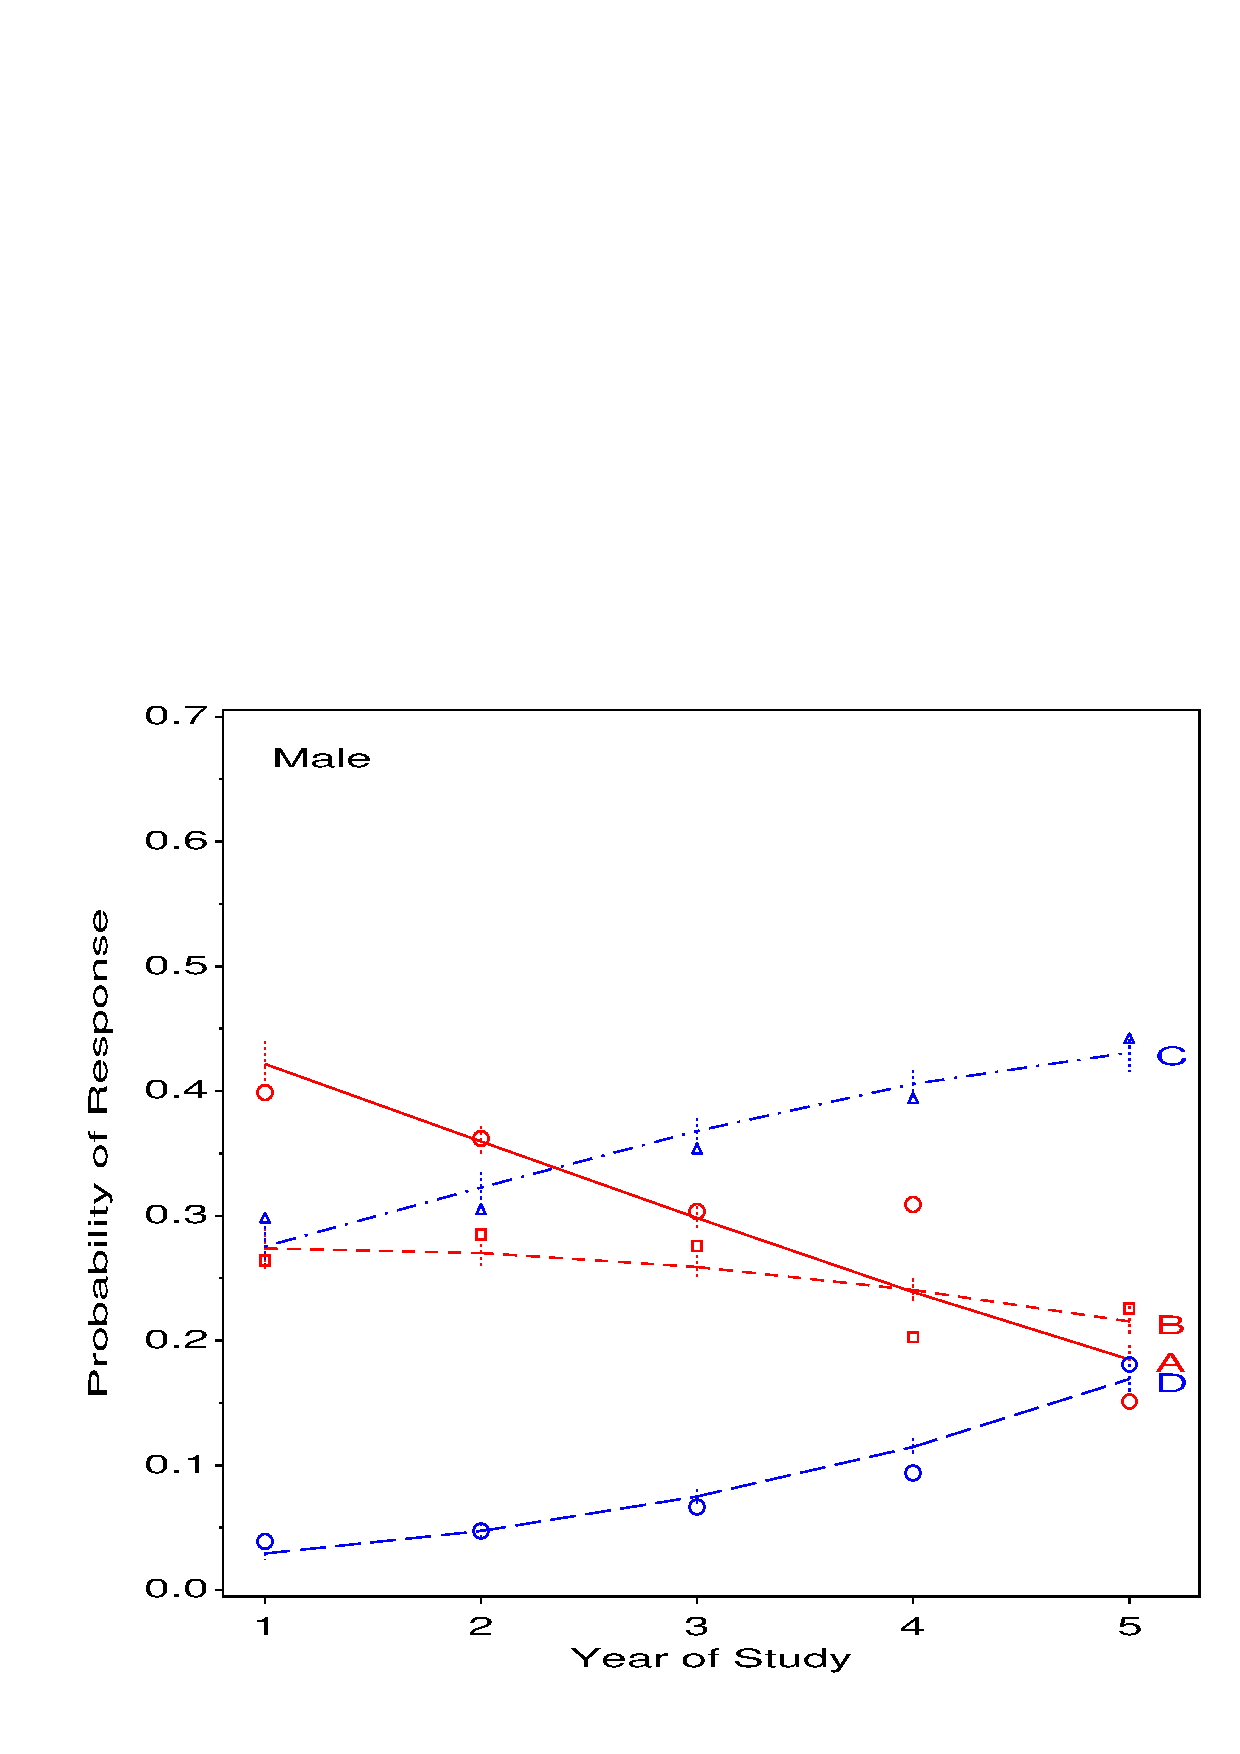
\includegraphics[width=1\linewidth]{vietnam22}
 \end{minipage}
 \caption{Observed and fitted probabilities for model $R = S + Y_{lin}(M)$}\label{fig:vietnam2}
\end{figure}
\end{Example}

\subsection{A fresh look}
Plots of observed and fitted values can tell part of the story,
but it is the \emph{comparison} of the two, in relation to the structure of
the data, which is most effective in suggesting ways to modify a
given model.  Probability plots or index plots of residuals can be useful,
but these do not relate to the structure of the contingency table
or to the pattern of association.
Mosaic displays and \CA\ are more useful for understanding the nature of associations,
which they reveal in different ways.

\begin{Example}[vietnam2]{Student opinion about the Vietnam war}
Because we have seen that the associations of response with year
differ for men and women, it is natural to examine partial mosaic
plots for the two sexes.
This is easily done with the \macro{MOSAIC}, using \pname{by=sex}.
First, a \Dstp\ is used to create more meaningful labels for
\pname{response} and \pname{year}. These statements create the two
graphs shown in \figref{fig:mosviet}.
\subsection{A fresh look}
Plots of observed and fitted values can tell part of the story,
but it is the \emph{comparison} of the two, in relation to the structure of
the data, which is most effective in suggesting ways to modify a
given model.  Probability plots or index plots of residuals can be useful,
but these do not relate to the structure of the contingency table
or to the pattern of association.
Mosaic displays and \CA\ are more useful for understanding the nature of associations,
which they reveal in different ways.

\begin{Example}[vietnam2]{Student opinion about the Vietnam war}
Because we have seen that the associations of response with year
differ for men and women, it is natural to examine partial mosaic
plots for the two sexes.
This is easily done with the \macro{MOSAIC}, using \pname{by=sex}.
First, a \Dstp\ is used to create more meaningful labels for
\pname{response} and \pname{year}. These statements create the two
graphs shown in \figref{fig:mosviet}.
\subsection{A fresh look}
Plots of observed and fitted values can tell part of the story,
but it is the \emph{comparison} of the two, in relation to the structure of
the data, which is most effective in suggesting ways to modify a
given model.  Probability plots or index plots of residuals can be useful,
but these do not relate to the structure of the contingency table
or to the pattern of association.
Mosaic displays and \CA\ are more useful for understanding the nature of associations,
which they reveal in different ways.

\begin{Example}[vietnam2]{Student opinion about the Vietnam war}
Because we have seen that the associations of response with year
differ for men and women, it is natural to examine partial mosaic
plots for the two sexes.
This is easily done with the \macro{MOSAIC}, using \pname{by=sex}.
First, a \Dstp\ is used to create more meaningful labels for
\pname{response} and \pname{year}. These statements create the two
graphs shown in \figref{fig:mosviet}.
\input{ch7/sas/mosviet}

%% two subfig side-by-side
\begin{figure}[htb]
 \begin{minipage}[t]{.49\linewidth}
  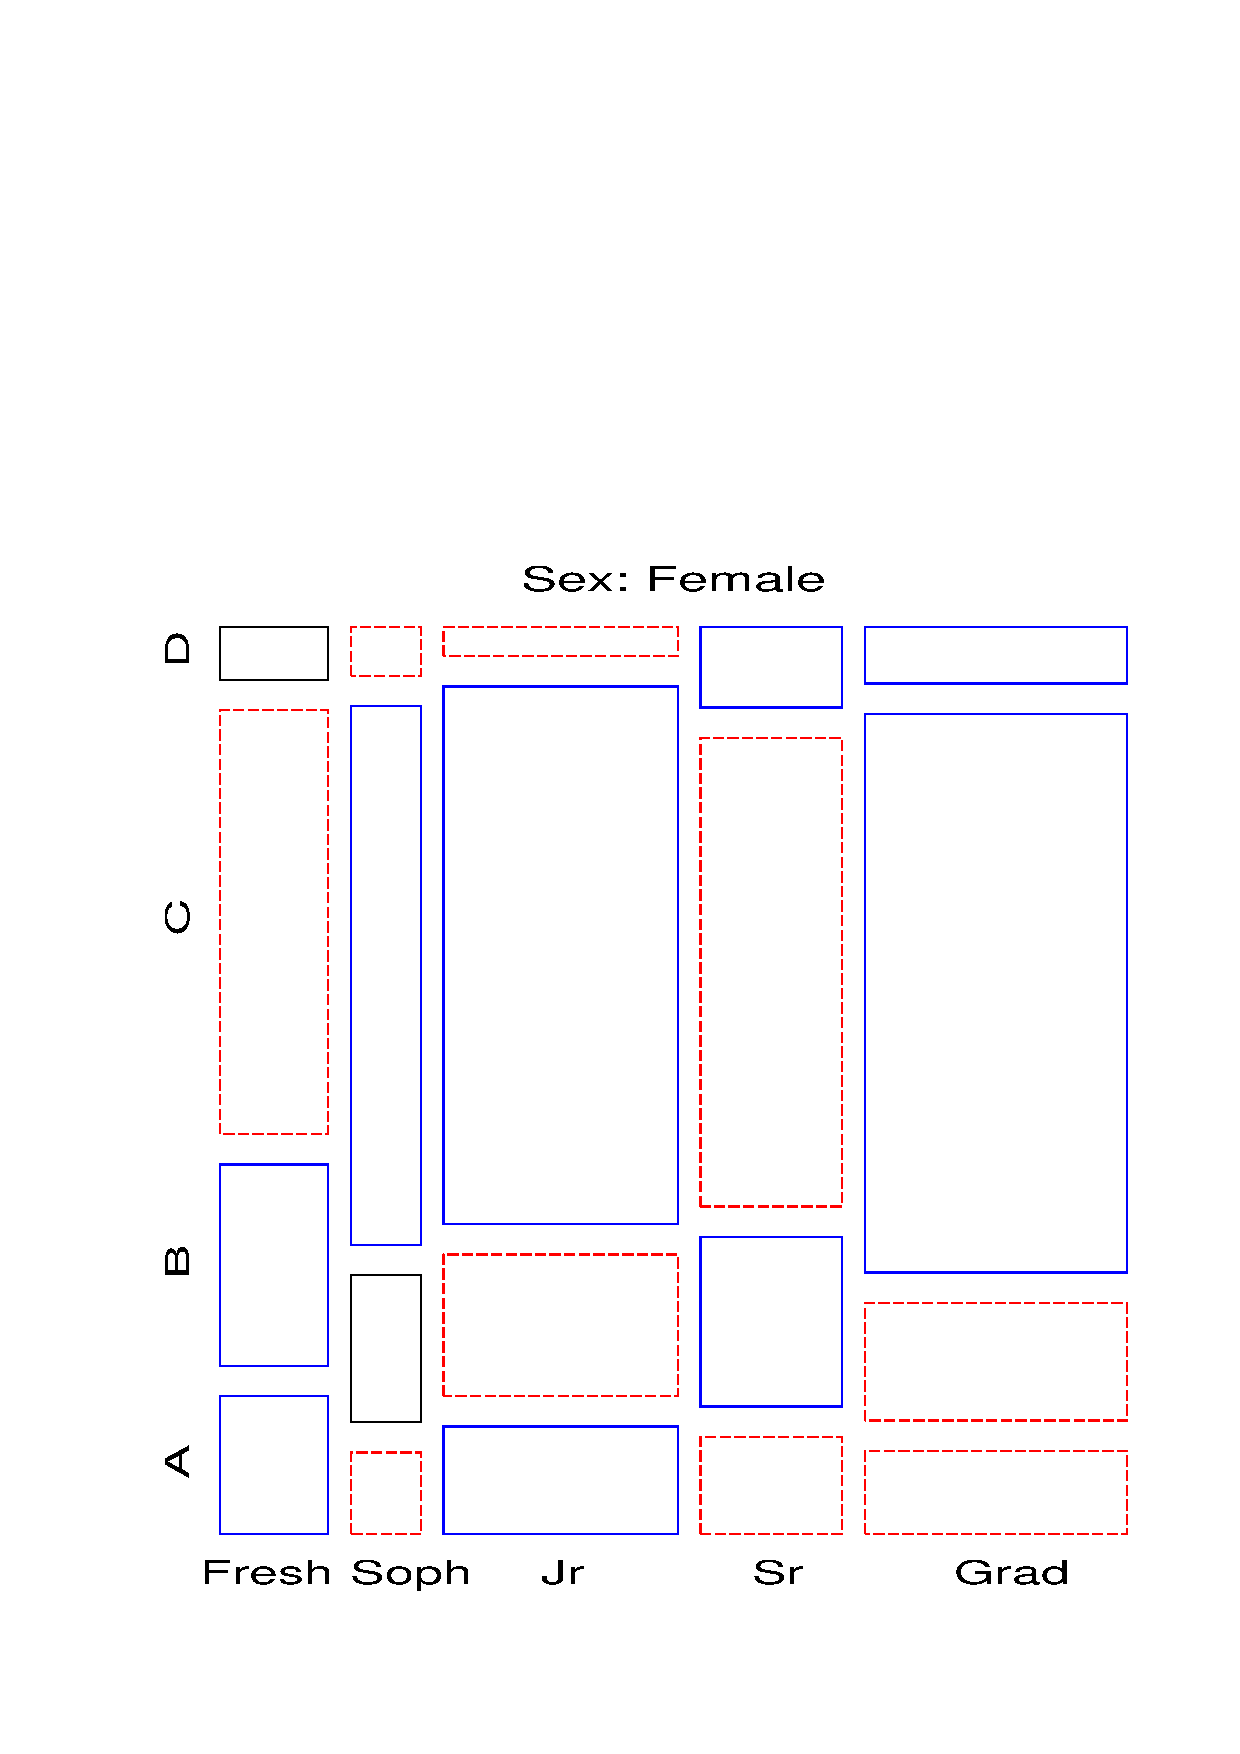
\includegraphics[width=1\linewidth,clip]{mosviet1}
 \end{minipage}%
 \hfill
 \begin{minipage}[t]{.49\linewidth}
  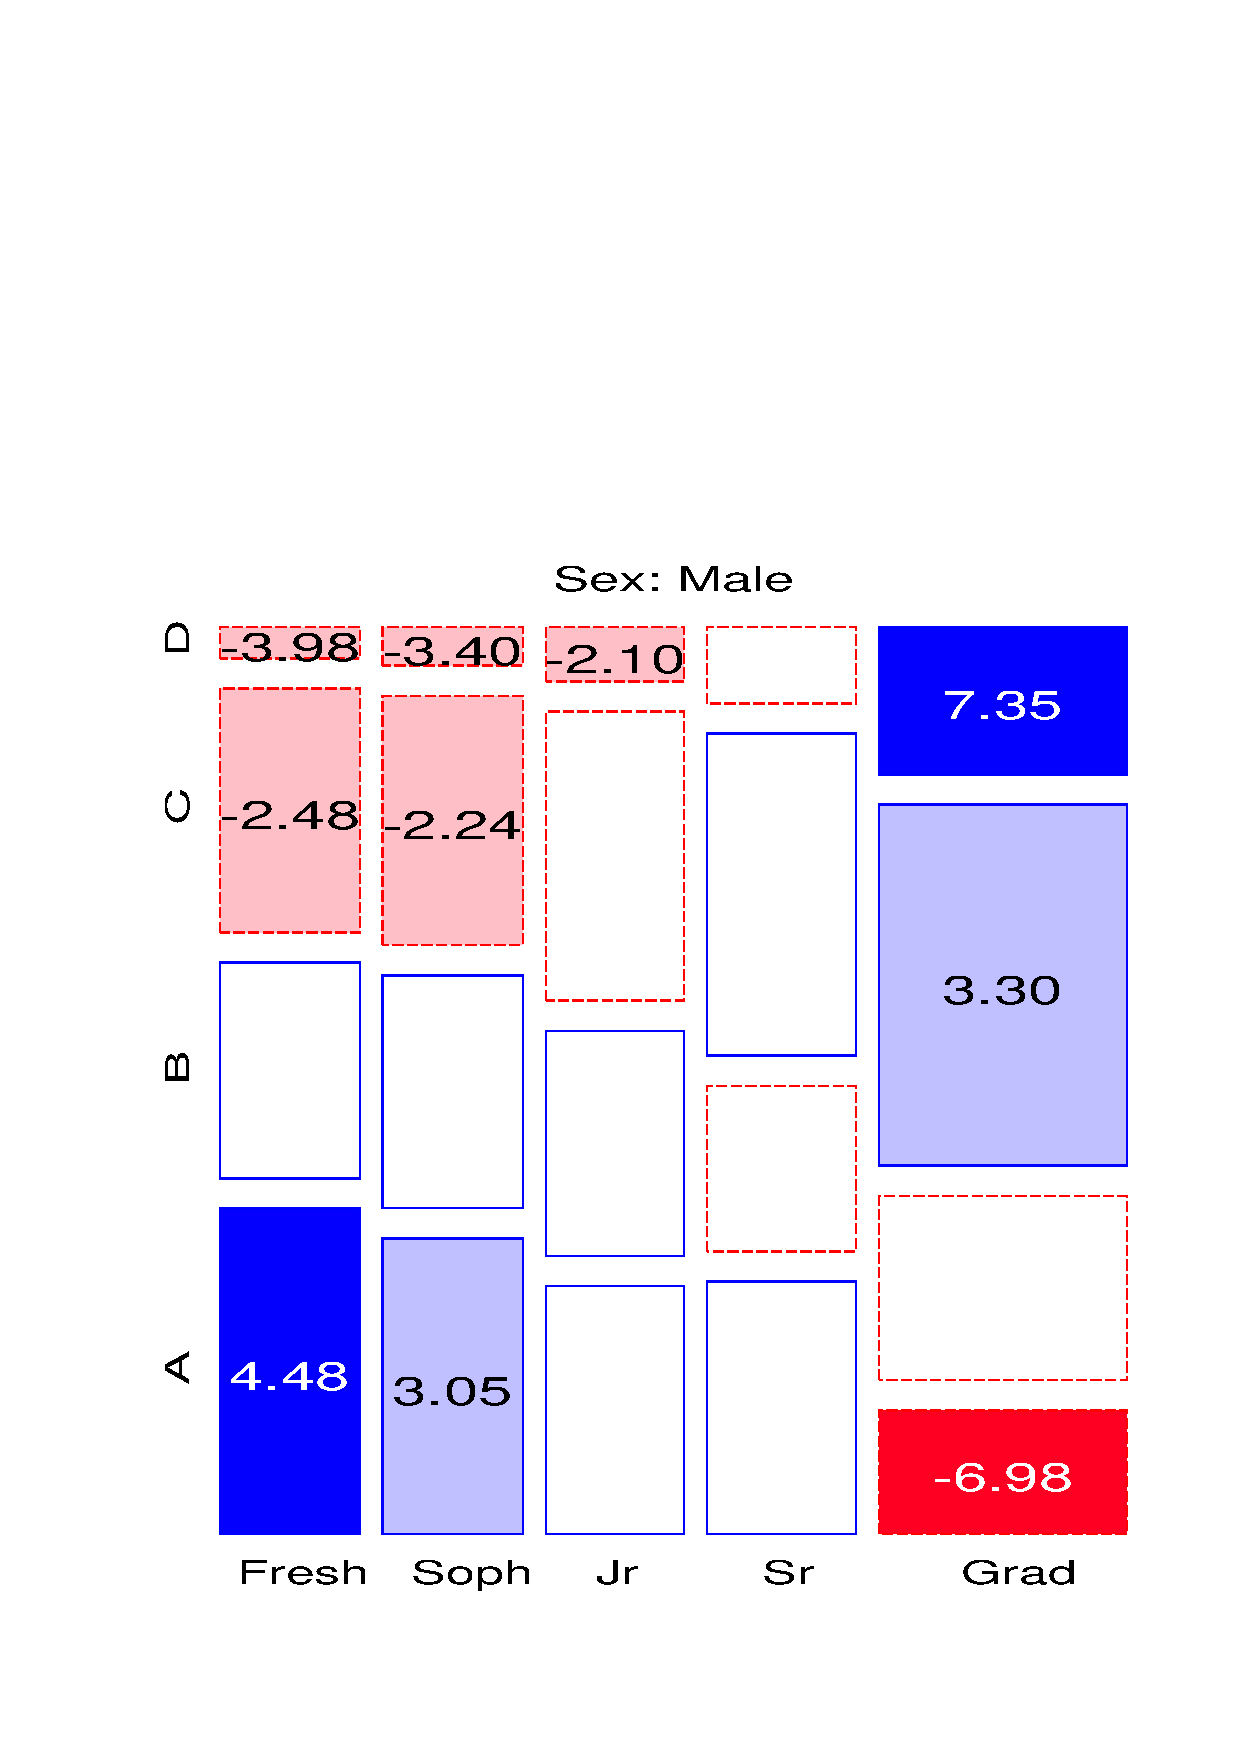
\includegraphics[width=1\linewidth,clip]{mosviet2}
 \end{minipage}
 \caption{Partial mosaic plots, by sex, for Vietnam war data}\label{fig:mosviet}
\end{figure}
With the variables in each mosaic ordered Year, Response,
recall that the height of each bar shows the (conditional) proportion
of students in each year who chose each response. There is no systematic
pattern for women, but the pattern of heights of the boxes, and of the
residuals from independence for men is very systematic.
The trend over years is easiest to see for responses A and D;
note that there is a large jump in proportion choosing these responses
between 4th year students and graduate students.
Perhaps our assumption of a linear trend with year for males needs
adjustment.

A \CA\ plot also displays residuals from a background model.  Here
we choose the null-response model of joint independence, $[SY] [R]$, so that all associations
between the response and the sex-year combinations will be shown.
To do this, we first transpose the data so that the responses
are columns and the sex-year populations are rows.
\begin{listing}
%include catdata(vietnam);

*-- Reshape to two-way table, SexYr x Response;
proc transpose data=vietnam prefix=R out=viet2way;
   var count;
   by sex year;

data viet2way;
   set viet2way;
   rename r1=A r2=B r3=C r4=D;
   sexyr = sex || put(year,1.);
   drop _name_;
proc print;

%corresp(data=viet2way, var=A--D, id=sexyr, interp=none join);
\end{listing}

The plot, shown in \figref{fig:vietcores} is quite revealing.
The response points, A--D
largely define the first dimension,
which accounts for 73.6\% of the association from the null-response model.
The year points for men, M1--M5,
are also ordered along this dimension, but male graduate students are far
from the male undergraduates.
The year points for women are tightly clustered, and aligned closest to
response C, their most preferred alternative.
The second dimension seems largely to do with the contrast between the relatively high choice for response D (``immediate withdrawal'')
among male graduate students and general preference for response C
(``de-escalate'') among most women.

%% one figure
\begin{figure}[htb]
  \centering
  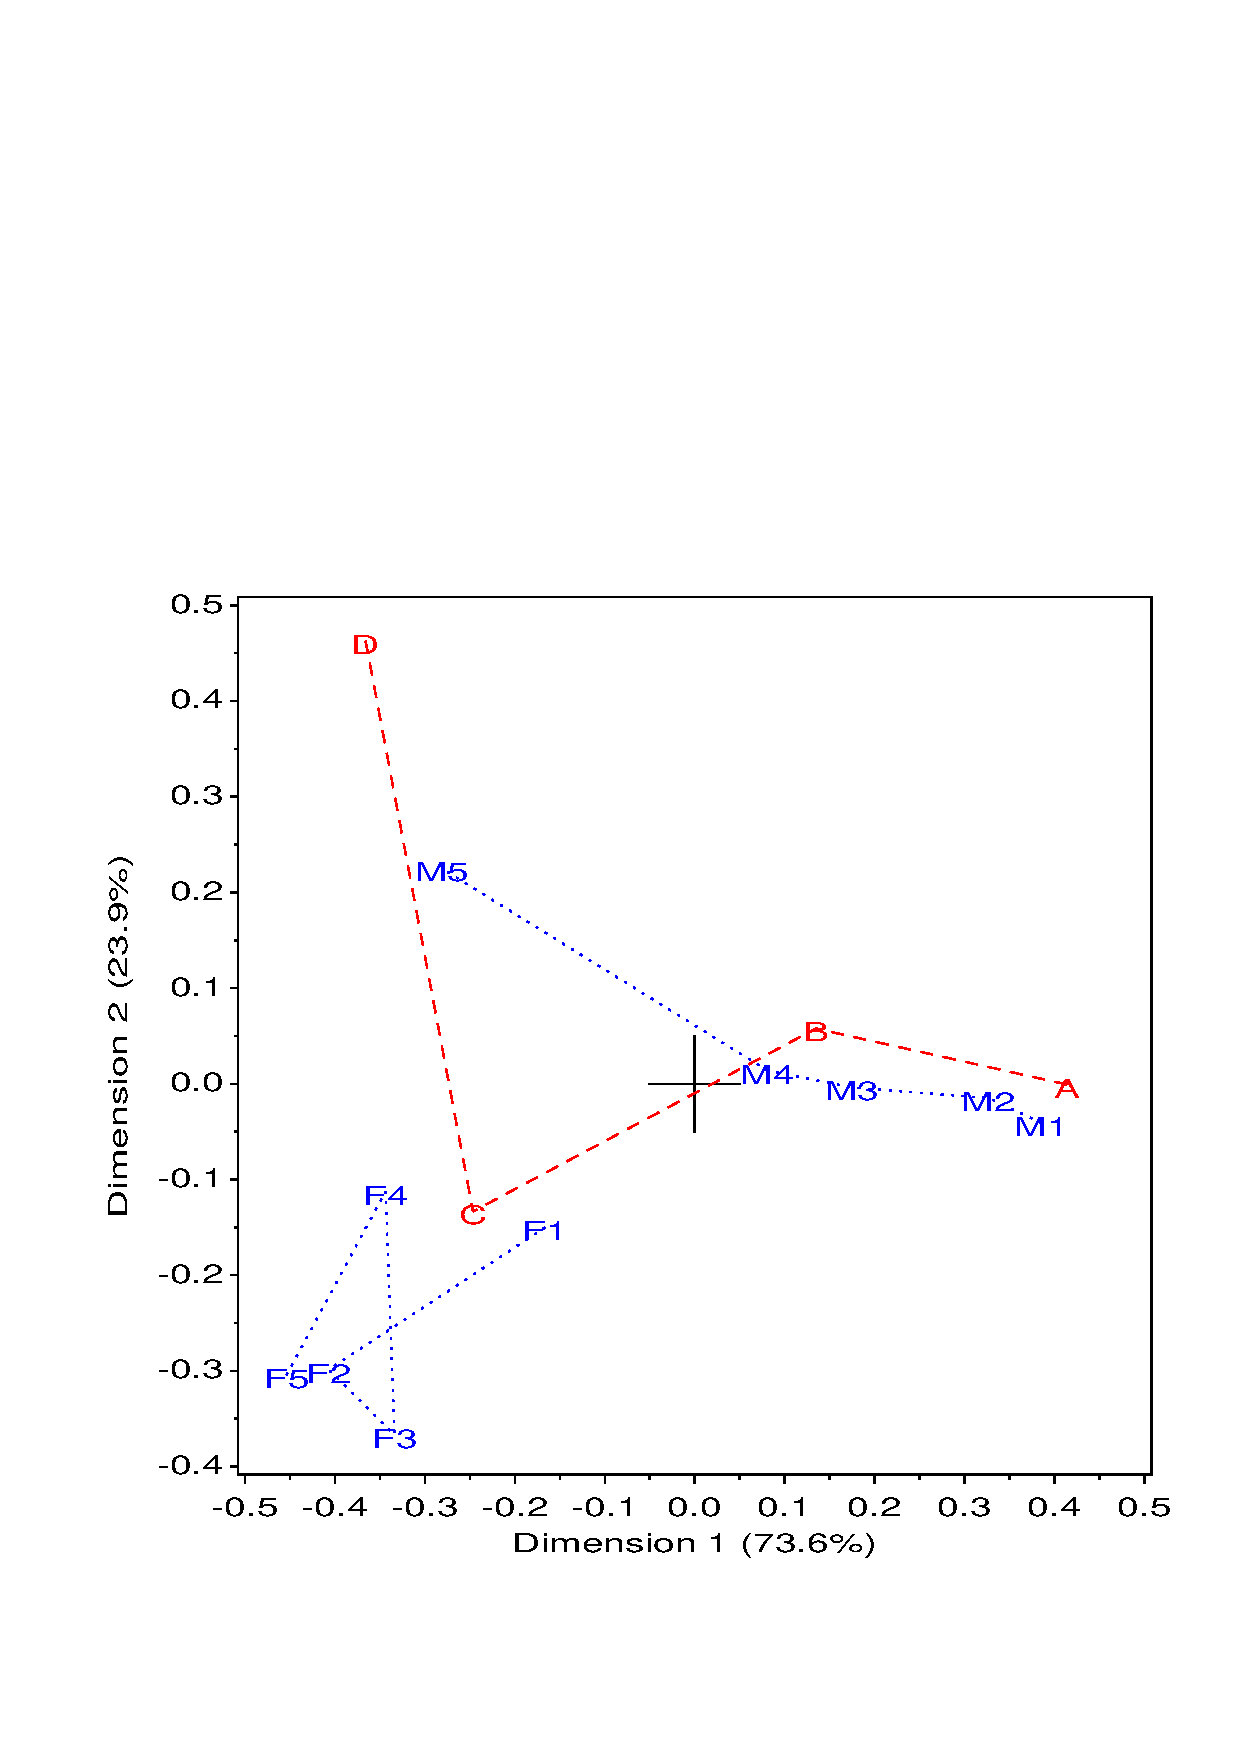
\includegraphics[scale=.6,clip]{vietcores}
  \caption{Correspondence analysis display for model $[SY][R]$}%
  \label{fig:vietcores}
\end{figure}

Both \figref{fig:mosviet} and \figref{fig:vietcores} indicate that our
assumption of linear spacing of year for men is incorrect, particularly
for graduate students.
A simple approach is to replace the variable \pname{year} with a new
variable, \pname{YR}, for which graduate students are some number
greater than 5.
Varying the year for graduate students over the range 5--10 gives
the residual \GSQ\ values (with 21 df)
in \tabref{tab:vietgrad}, and suggests that
7 years for graduate students gives the best fit.  The plot
of fitted and observed values under the revised model is shown in \figref{fig:vietnam3}.
\input{ch7/sas/vietnam3}
\input{ch7/tab/vietgrad}

%% two subfig side-by-side
\begin{figure}[htb]
 \begin{minipage}[t]{.49\linewidth}
  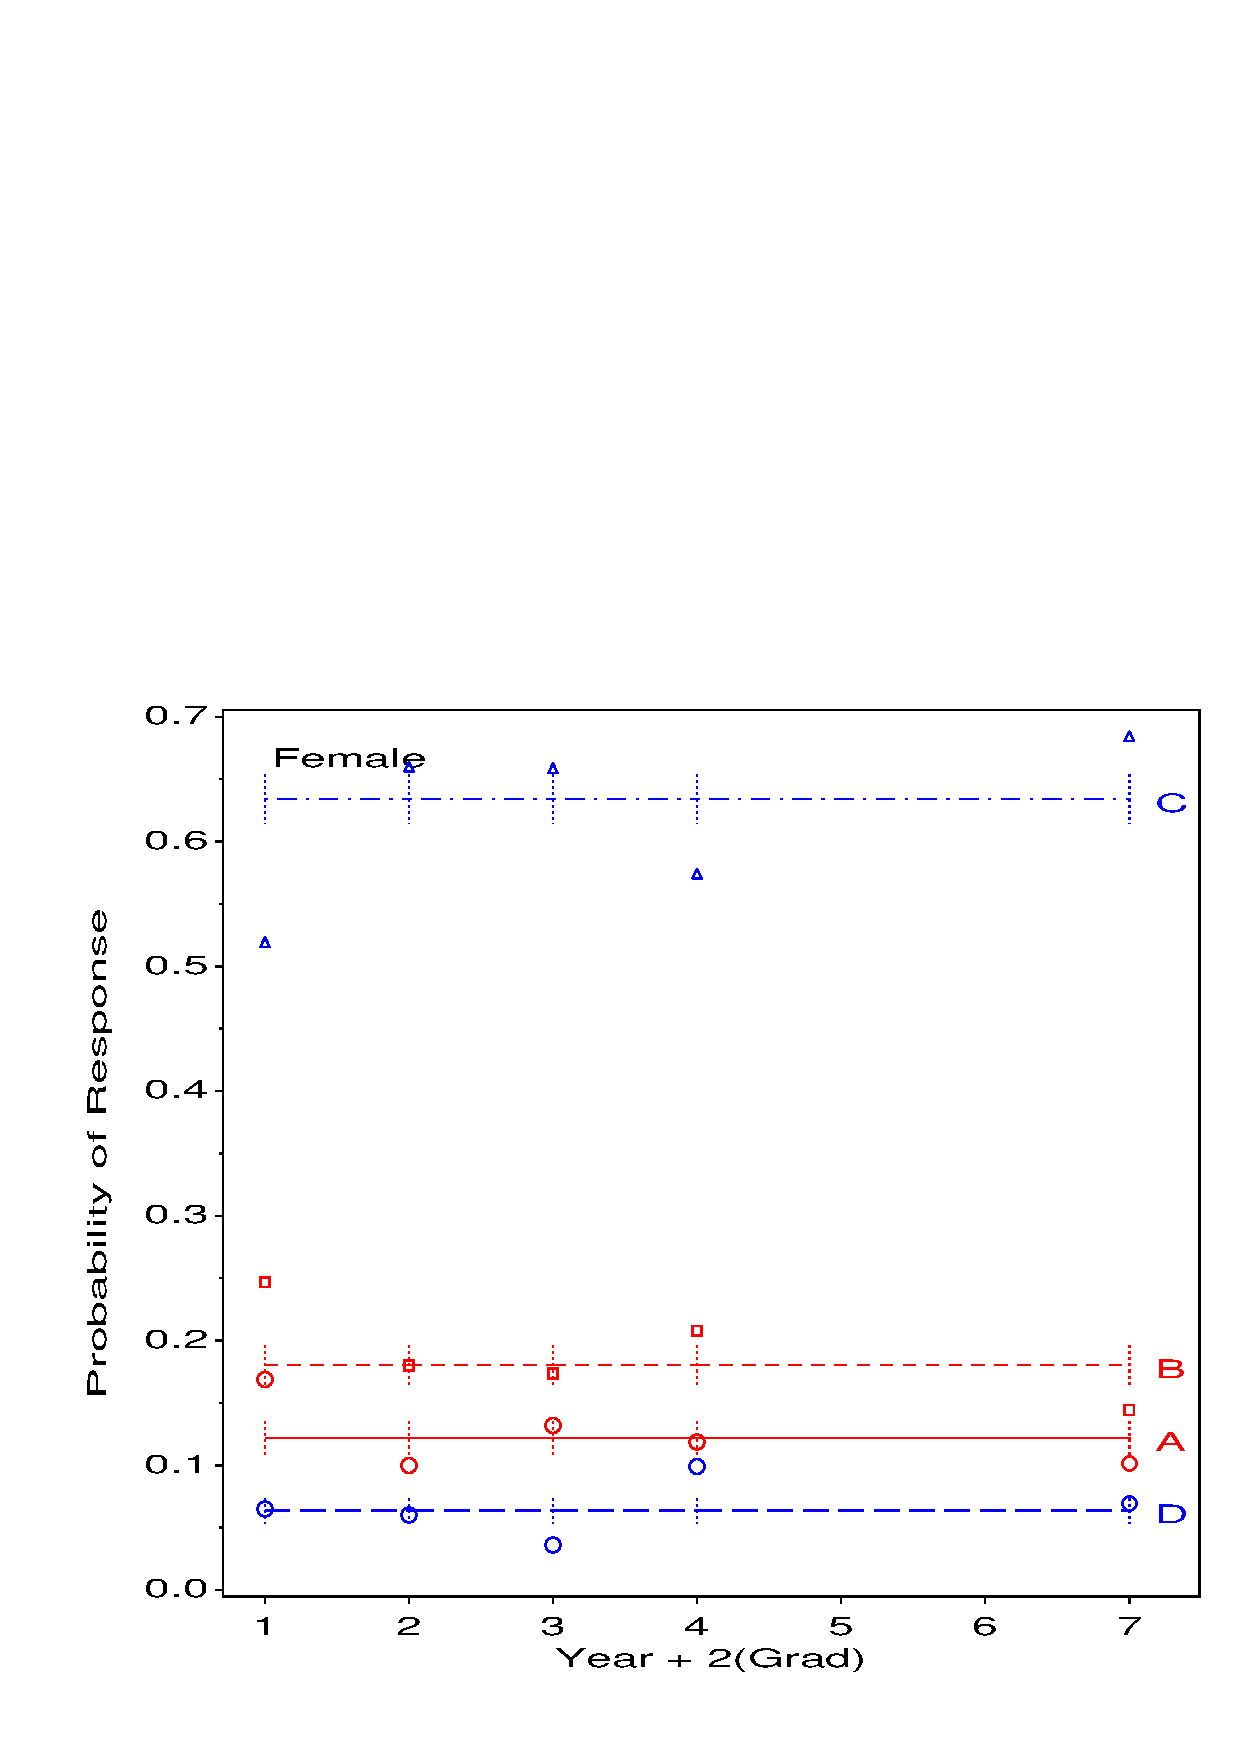
\includegraphics[width=1\linewidth]{vietnam31}
 \end{minipage}%
 \hfill
 \begin{minipage}[t]{.49\linewidth}
  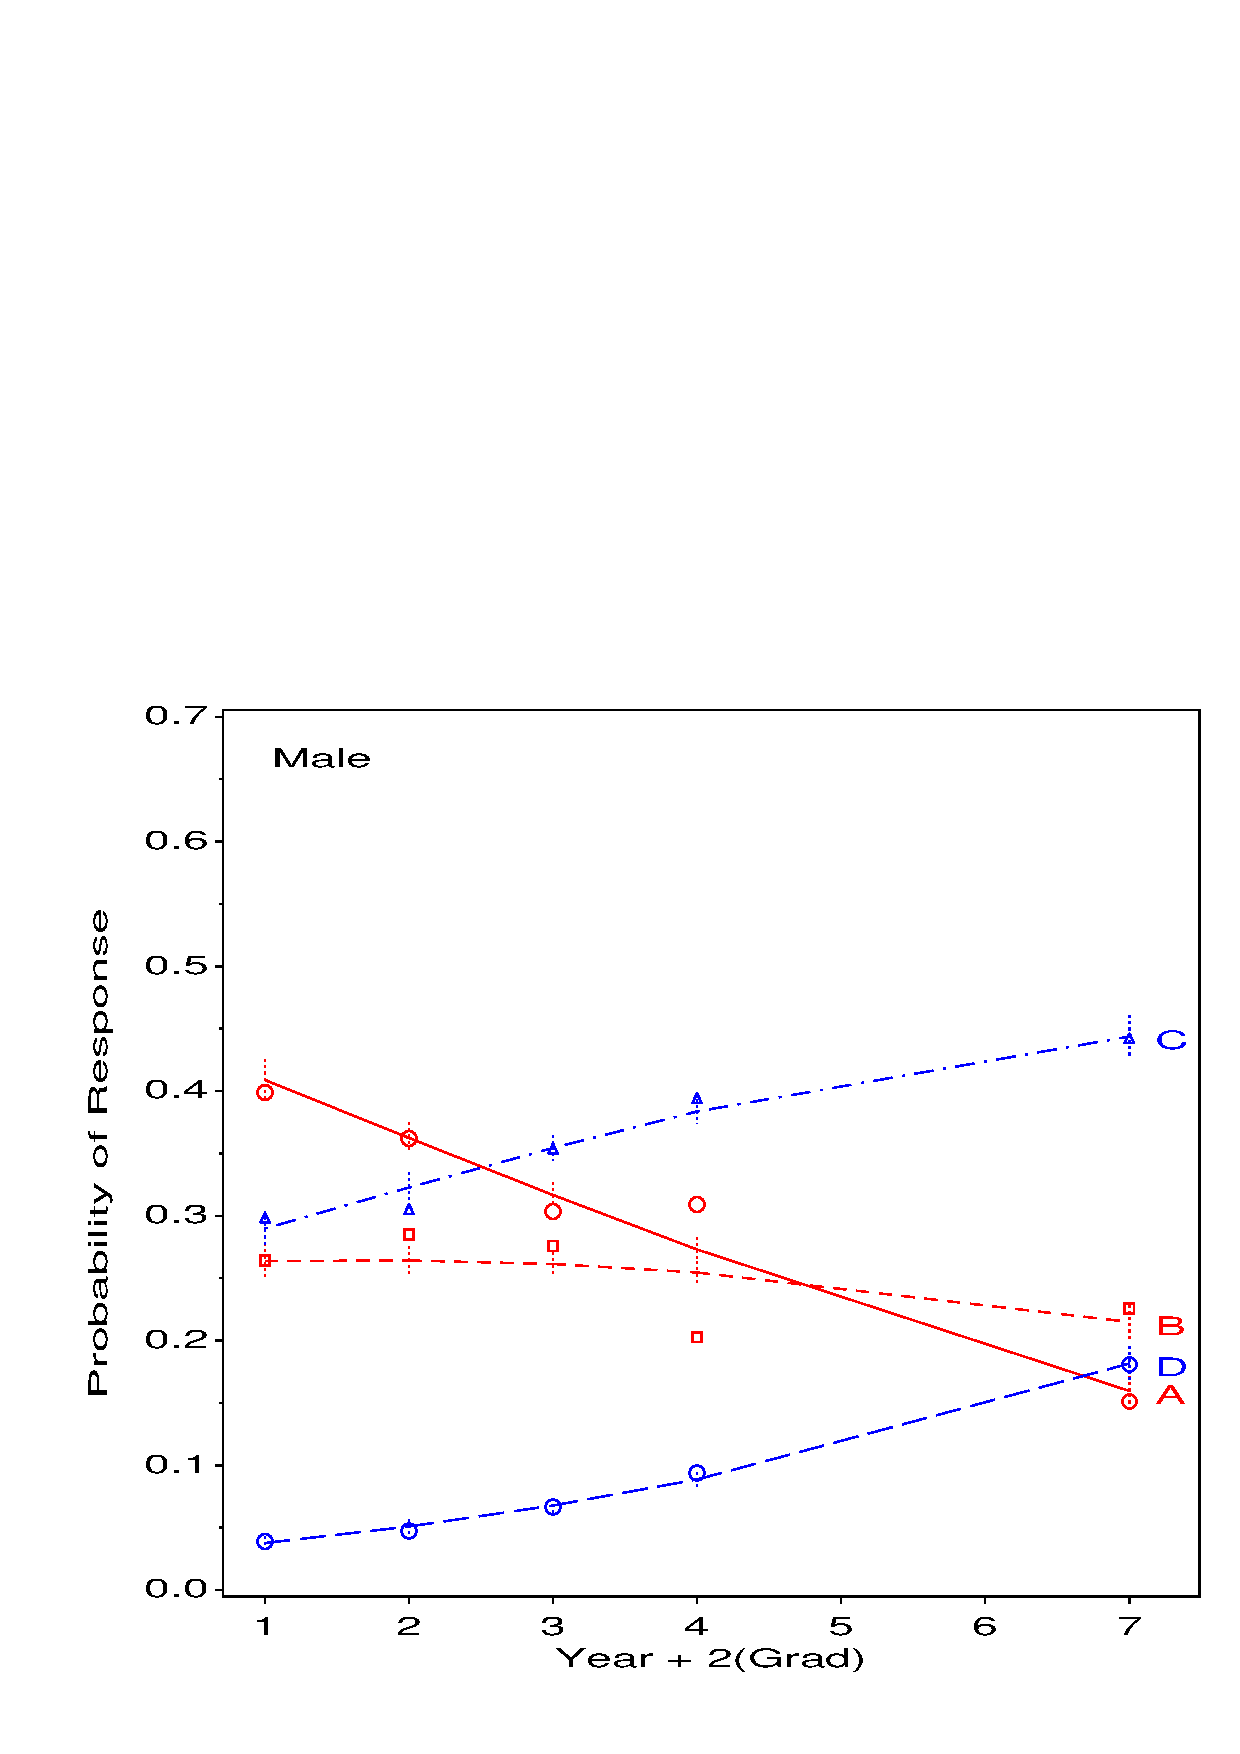
\includegraphics[width=1\linewidth]{vietnam32}
 \end{minipage}
 \caption{Observed and fitted probabilities for model $R = S + Y_{lin}(M)$, Graduate students=7}\label{fig:vietnam3}
\end{figure}

This model fits quite well overall, but there are still several
discrepant points.
We examine residuals and influence diagnostics for this model in
the following section
(\exref{ex:vietnam3}).
\end{Example}


%% two subfig side-by-side
\begin{figure}[htb]
 \begin{minipage}[t]{.49\linewidth}
  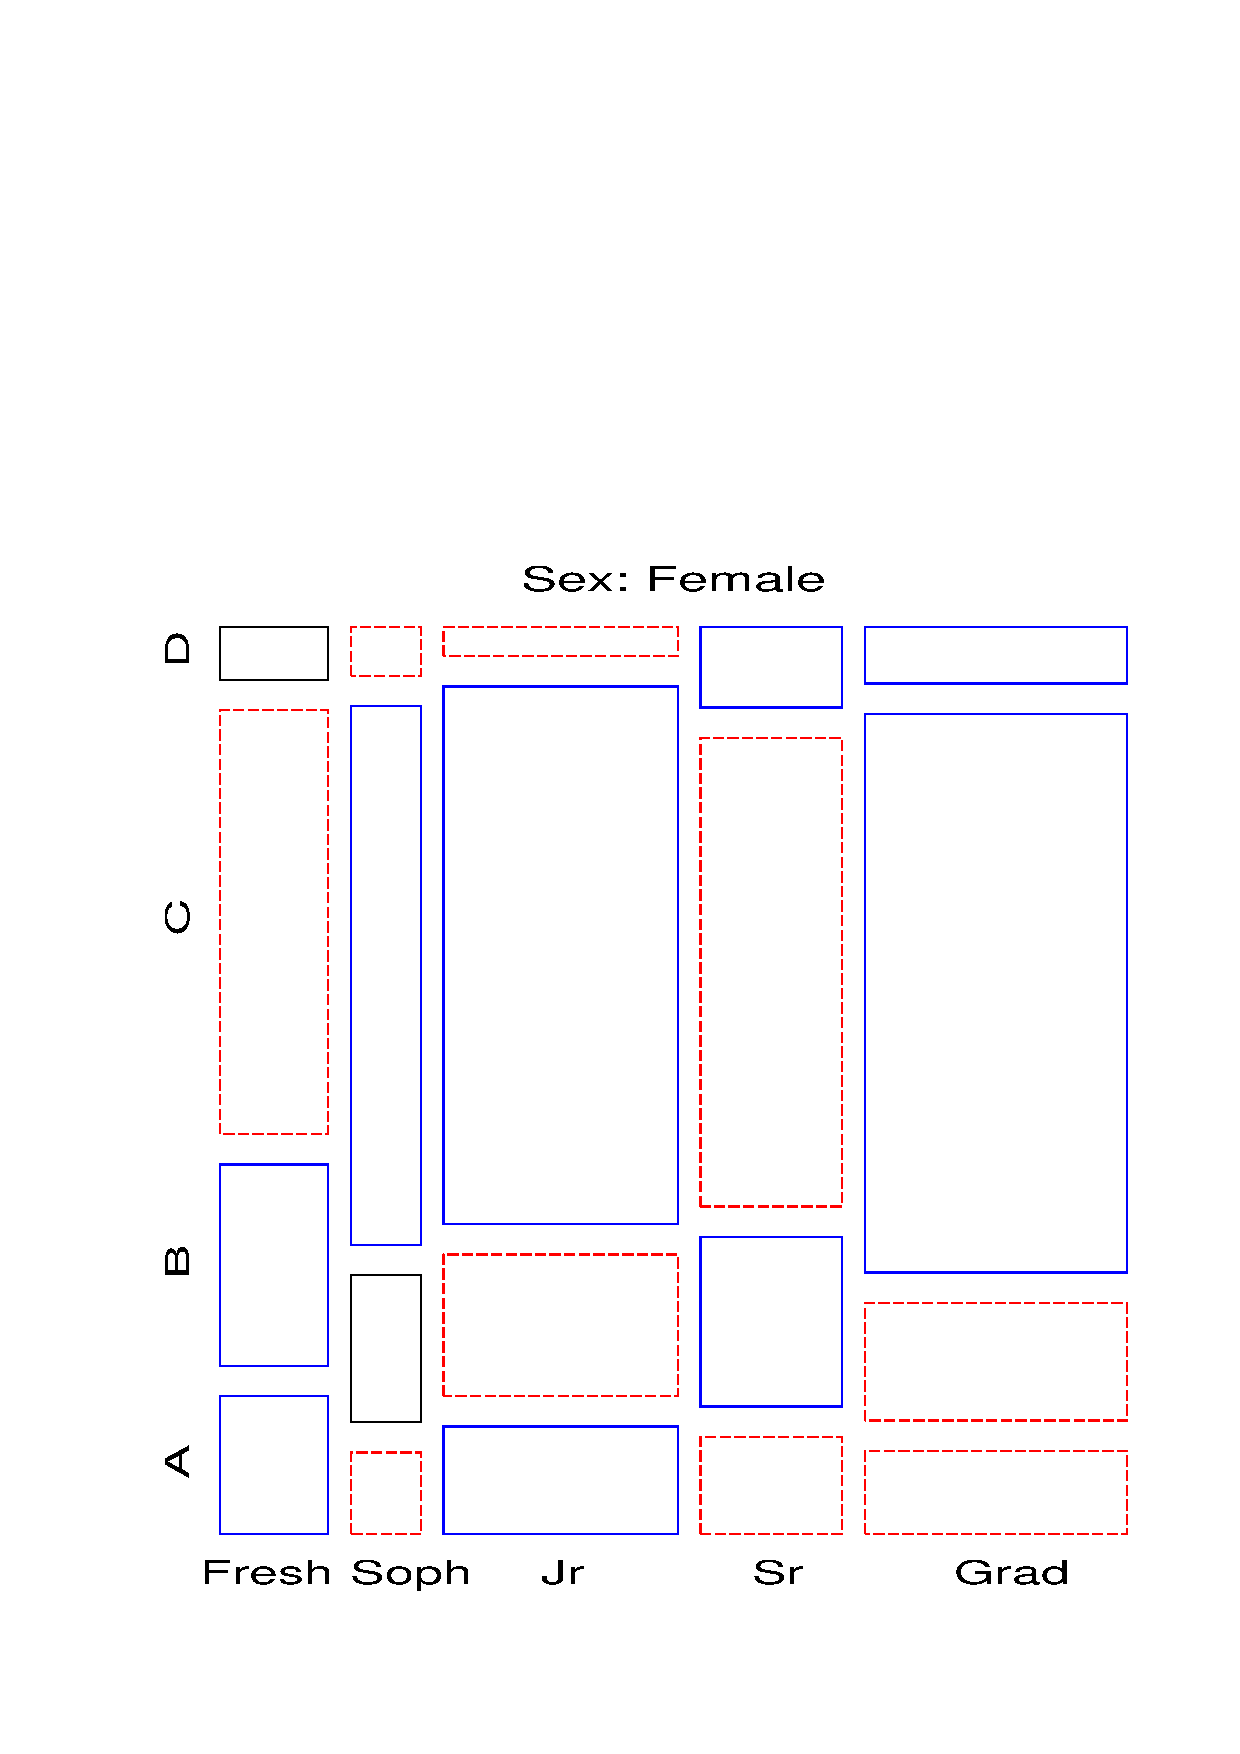
\includegraphics[width=1\linewidth,clip]{mosviet1}
 \end{minipage}%
 \hfill
 \begin{minipage}[t]{.49\linewidth}
  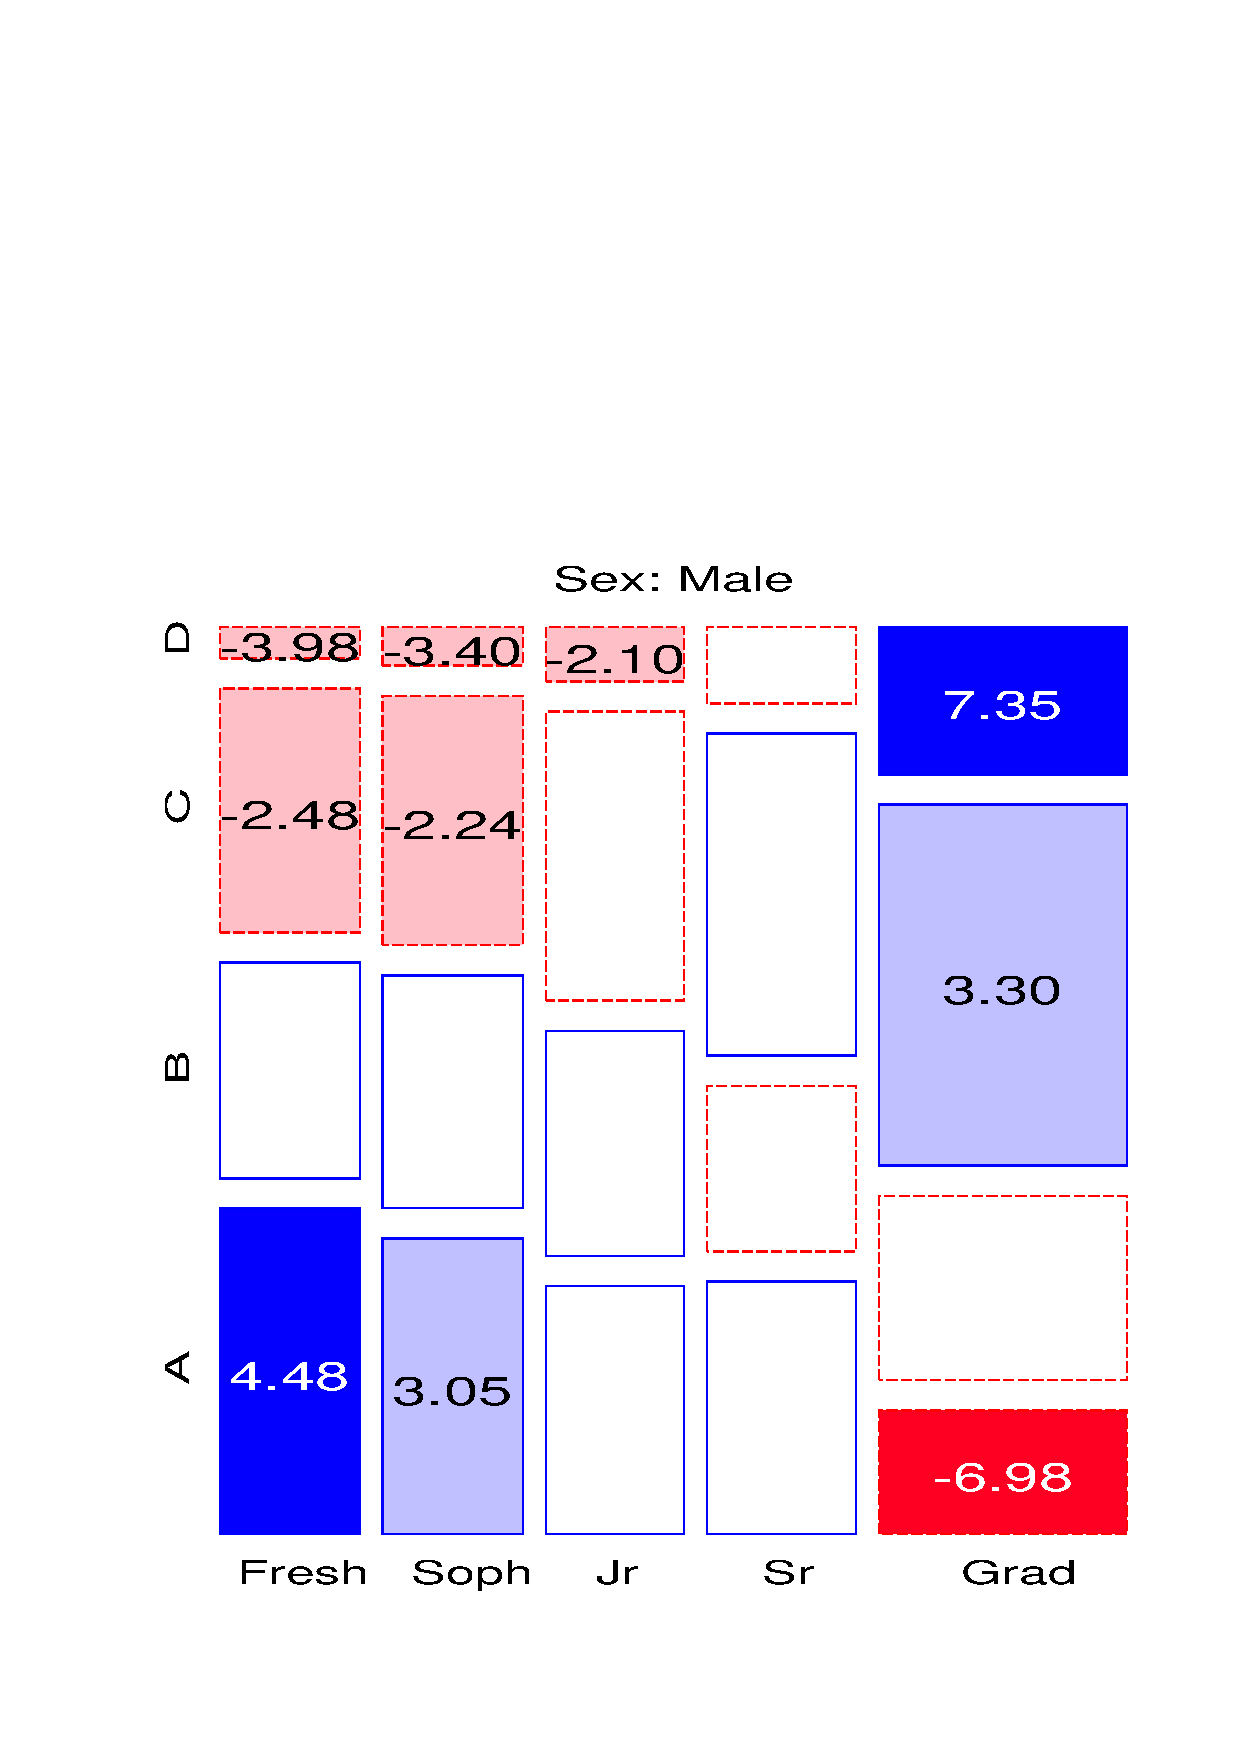
\includegraphics[width=1\linewidth,clip]{mosviet2}
 \end{minipage}
 \caption{Partial mosaic plots, by sex, for Vietnam war data}\label{fig:mosviet}
\end{figure}
With the variables in each mosaic ordered Year, Response,
recall that the height of each bar shows the (conditional) proportion
of students in each year who chose each response. There is no systematic
pattern for women, but the pattern of heights of the boxes, and of the
residuals from independence for men is very systematic.
The trend over years is easiest to see for responses A and D;
note that there is a large jump in proportion choosing these responses
between 4th year students and graduate students.
Perhaps our assumption of a linear trend with year for males needs
adjustment.

A \CA\ plot also displays residuals from a background model.  Here
we choose the null-response model of joint independence, $[SY] [R]$, so that all associations
between the response and the sex-year combinations will be shown.
To do this, we first transpose the data so that the responses
are columns and the sex-year populations are rows.
\begin{listing}
%include catdata(vietnam);

*-- Reshape to two-way table, SexYr x Response;
proc transpose data=vietnam prefix=R out=viet2way;
   var count;
   by sex year;

data viet2way;
   set viet2way;
   rename r1=A r2=B r3=C r4=D;
   sexyr = sex || put(year,1.);
   drop _name_;
proc print;

%corresp(data=viet2way, var=A--D, id=sexyr, interp=none join);
\end{listing}

The plot, shown in \figref{fig:vietcores} is quite revealing.
The response points, A--D
largely define the first dimension,
which accounts for 73.6\% of the association from the null-response model.
The year points for men, M1--M5,
are also ordered along this dimension, but male graduate students are far
from the male undergraduates.
The year points for women are tightly clustered, and aligned closest to
response C, their most preferred alternative.
The second dimension seems largely to do with the contrast between the relatively high choice for response D (``immediate withdrawal'')
among male graduate students and general preference for response C
(``de-escalate'') among most women.

%% one figure
\begin{figure}[htb]
  \centering
  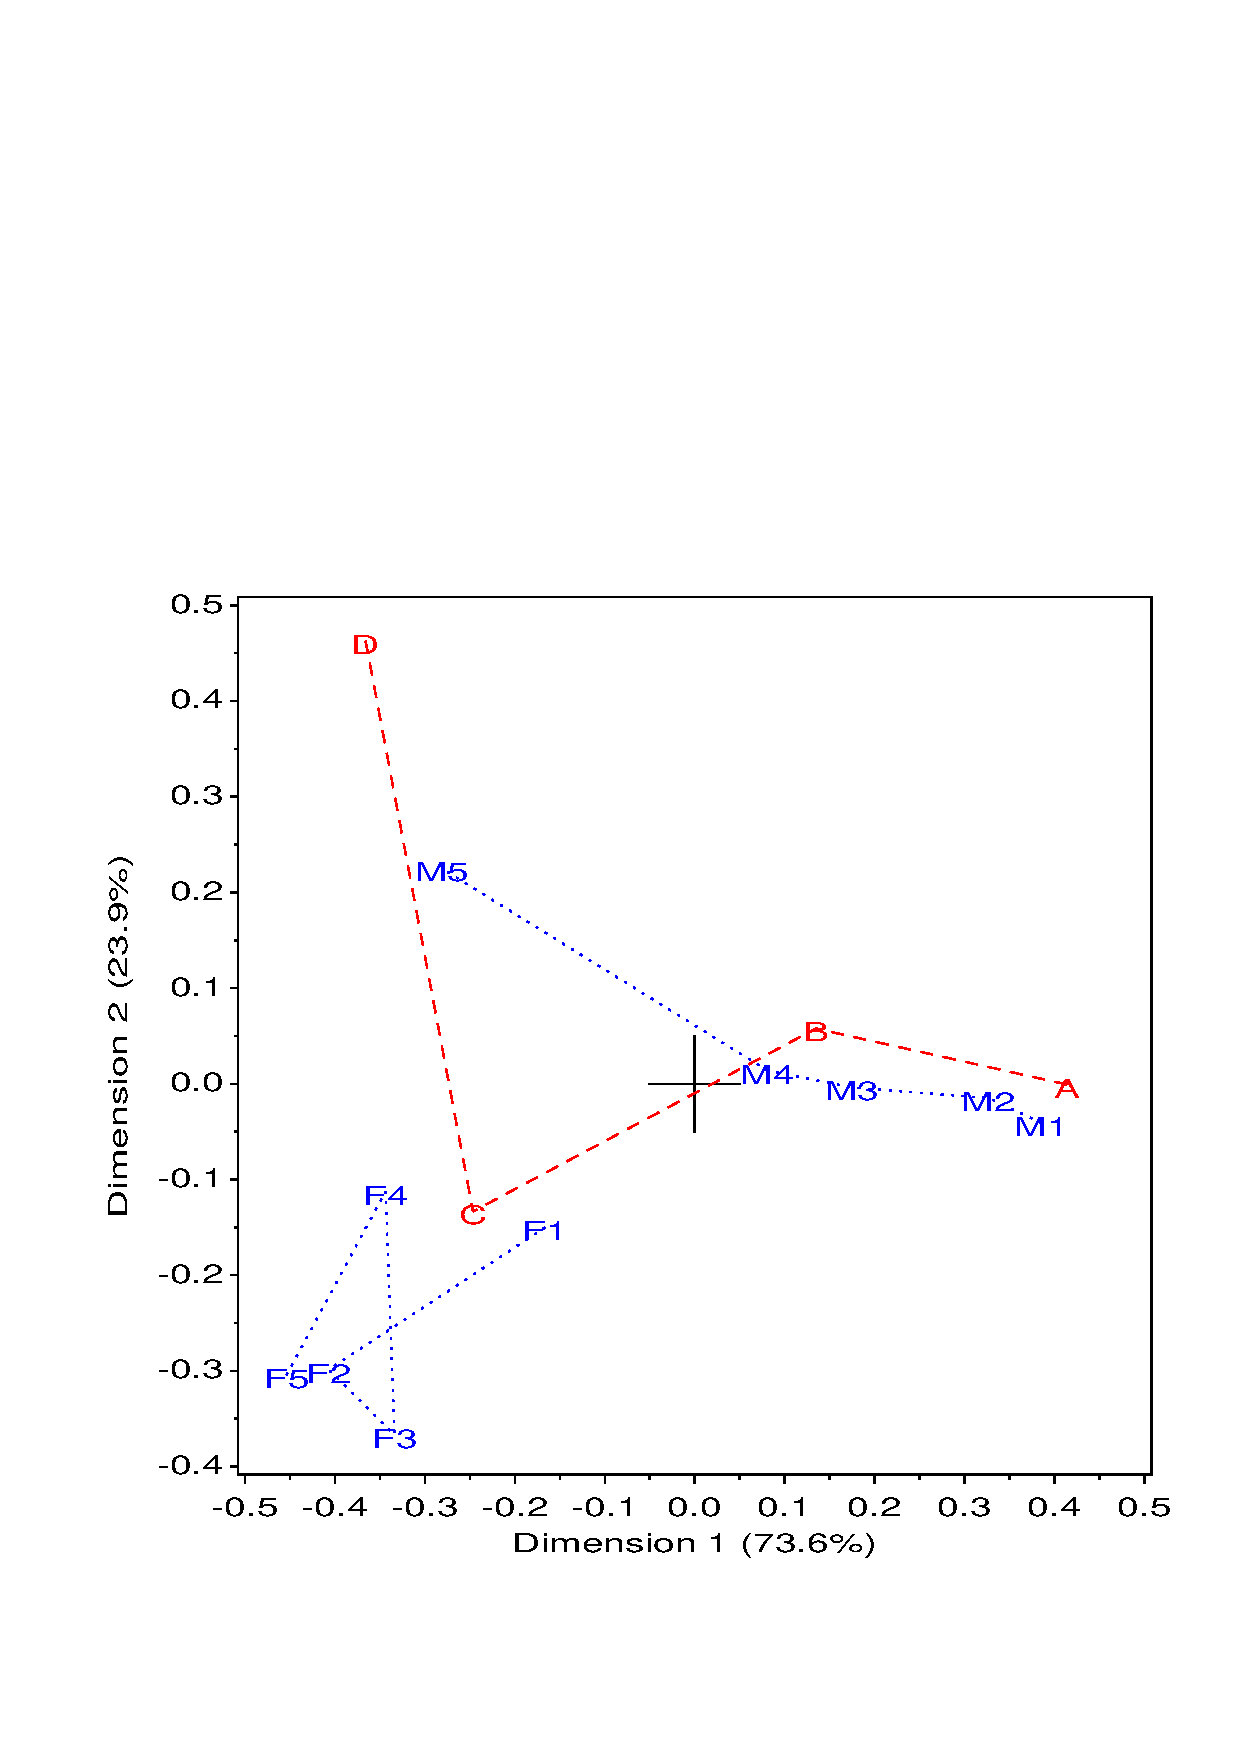
\includegraphics[scale=.6,clip]{vietcores}
  \caption{Correspondence analysis display for model $[SY][R]$}%
  \label{fig:vietcores}
\end{figure}

Both \figref{fig:mosviet} and \figref{fig:vietcores} indicate that our
assumption of linear spacing of year for men is incorrect, particularly
for graduate students.
A simple approach is to replace the variable \pname{year} with a new
variable, \pname{YR}, for which graduate students are some number
greater than 5.
Varying the year for graduate students over the range 5--10 gives
the residual \GSQ\ values (with 21 df)
in \tabref{tab:vietgrad}, and suggests that
7 years for graduate students gives the best fit.  The plot
of fitted and observed values under the revised model is shown in \figref{fig:vietnam3}.
\begin{Example}[vietnam3]{Student opinion about the Vietnam war}
The revised model, with linear effects of year on each logit,
and with graduate students treated as \pname{yr=7}
 shown in \figref{fig:vietnam3} was fit using
\PROC{CATMOD}.  However, influence diagnostics are
easier to obtain using
\PROC{GENMOD}.
The same model can be fit using \PROC{GENMOD} by defining a dummy variable
for women and an interaction between \pname{yr} and a dummy variable
for men.
\begin{listing}
data vietnam;
   set vietnam;
   yr = year + 2*(year=5);
   mlin =  yr * (sex='M');
   female = (sex='F');
   cell = trim(sex)|| put(year,1.)|| trim(put(response,letter.));
   label yr="Year + 2(Grad)";

proc genmod data=vietnam;
   class year sex response;
   model count = year|sex response|mlin  response|female /
         dist=poisson obstats residuals;
   make 'obstats' out=obstats;
\end{listing}
Normally, one would need to merge the input \Dset\ with the \pname{obstats},
and calculate hat values, Cook's D or other quantities for plotting:
\begin{listing}
%let k=8;
data obstats;
   merge vietnam obstats;
   h = hesswgt * std**2;
   cookd = streschi**2 * h/((1-h) * &k);
\end{listing}
where \pname{k=8} is the number of estimated parameters.

Instead, the \macro{INFLGLIM} (\macref{mac:inflglim}) automates these steps, and
gives various influence plots of residuals from a given
model.  The macro plots all combinations of the variables given
by the \mparm{GY}{INFLGLIM} against the variables given by the \mparm{GX}{INFLGLIM},
using a bubble symbol whose size is proportional to the
\mparm{BUBBLE}{INFLGLIM}, usually Cook's D.

Here, we plot the one-step estimates of change in deviance
($\Delta G_{(-i)}^2$, or \pname{DIFDEV})
due to deleting each cell against hat values,
using bubble symbols with area proportional to Cook's D.
The \mparm{infl}{INFLGLIM} determines the criterion for labeling
potentially influential points.
\begin{listing}
%inflglim(data=vietnam, resp=count,
    class=year sex response,
    model= year|sex  response|mlin  response|female,
    dist=poisson, id=cell,
    infl=%str(difdev>4 or &bubble>1 or hat>1.5*&hcrit),
    gy=difdev, gx=hat, bubble=cookd);
\end{listing}

This plot (\figref{fig:vietgen3}) shows that there are still two
large residuals: 4th year men choose response B substantially less often
than predicted (accounting for over one-third of the model deviance), and first year women choose response C less than
predicted.
%% one figure
\begin{figure}[htb]
  \centering
  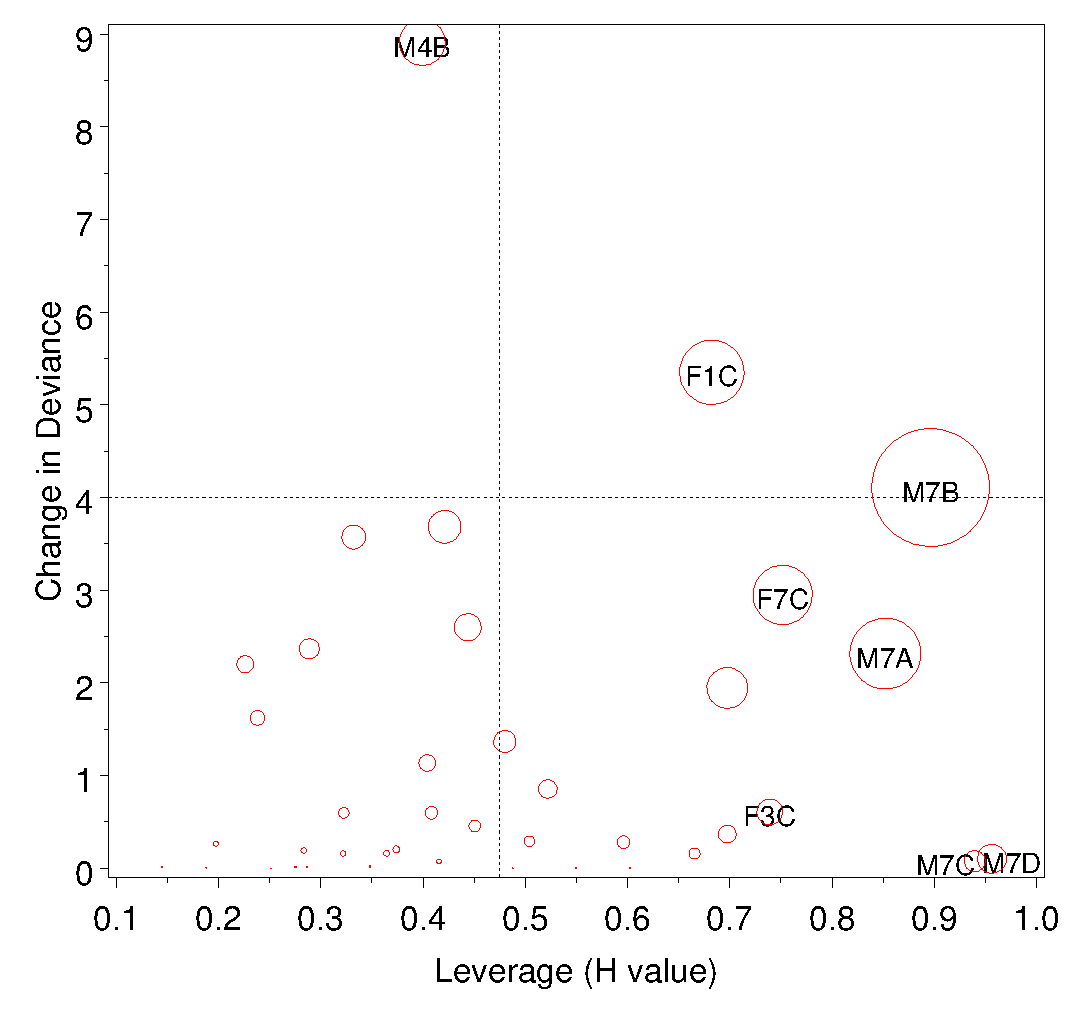
\includegraphics[scale=.6]{vietgen3}
  \caption{Influence plot for model $R = S + Y_{lin}(M)$, Graduate students=7}%
  \label{fig:vietgen3}
\end{figure}
We complete the analysis and this example with a half-normal plot of
these residuals, shown in \figref{fig:vietgen4}.  Although there is
evidence of non-normality in the distribution of residuals,  even the largest
values are within the simulated envelope.
\begin{listing}
%halfnorm(data=vietnam, resp=count,
   class=sex year response,
   model=year|sex  response|mlin  response|female,
   dist=poisson, id=cell);
\end{listing}

\begin{figure}[htb]
  \centering
  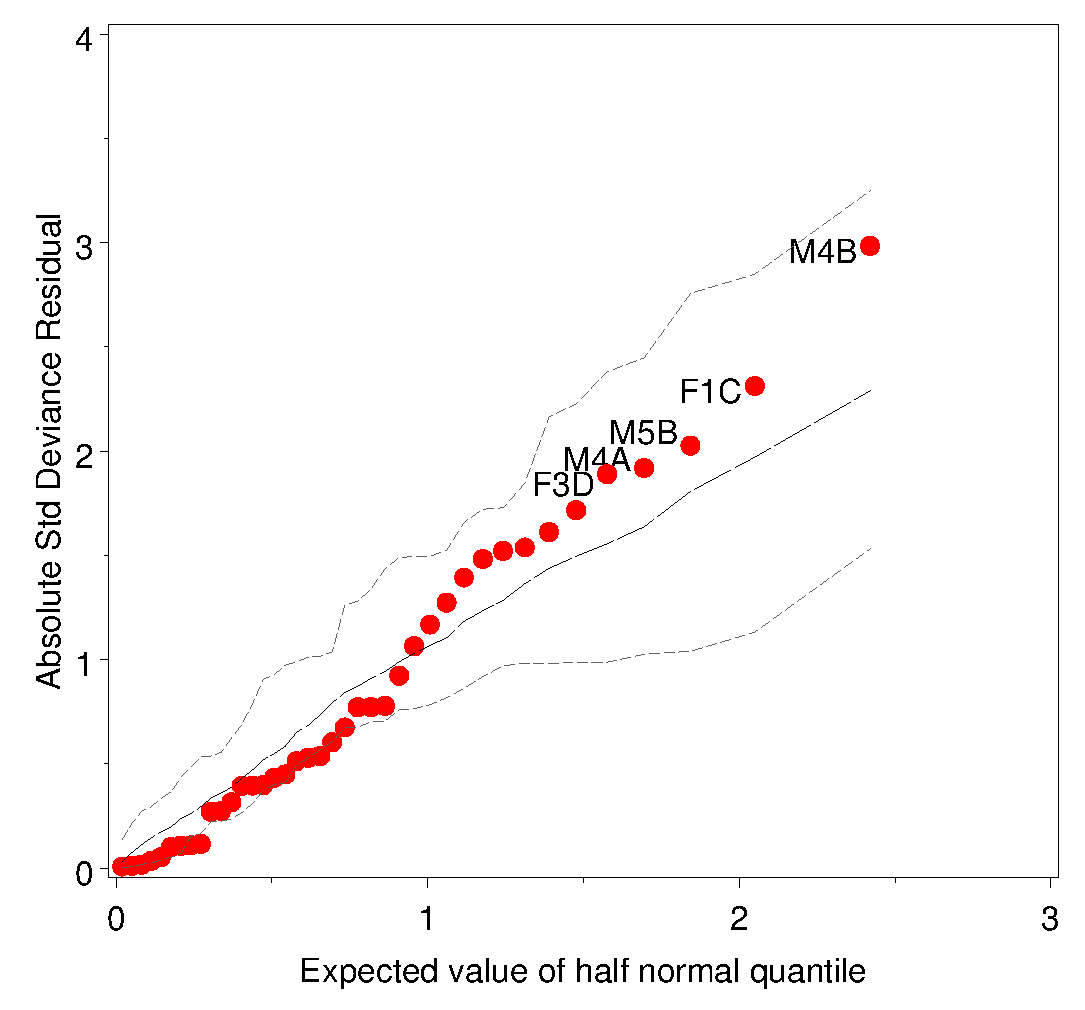
\includegraphics[scale=.6]{vietgen4}
  \caption{Half-normal plot for model $R = S + Y_{lin}(M)$, Graduate students=7}%
  \label{fig:vietgen4}
\end{figure}
\end{Example}

\begin{table}[htb]
 \caption{Profile deviance analysis of Year for Graduate Students}\label{tab:vietgrad}
 \begin{center}
 \begin{tabular}{cr}
  \hline
  Grad Year & \GSQ (21) \\
  \hline
  5 &  38.10 \\ 
  6 &  26.69 \\ 
  7 &  23.87 \\ 
  8 &  23.99 \\ 
  9 &  25.13 \\ 
  10 & 26.58 \\ 
  \hline
 \end{tabular}
 \end{center}
\end{table}


%% two subfig side-by-side
\begin{figure}[htb]
 \begin{minipage}[t]{.49\linewidth}
  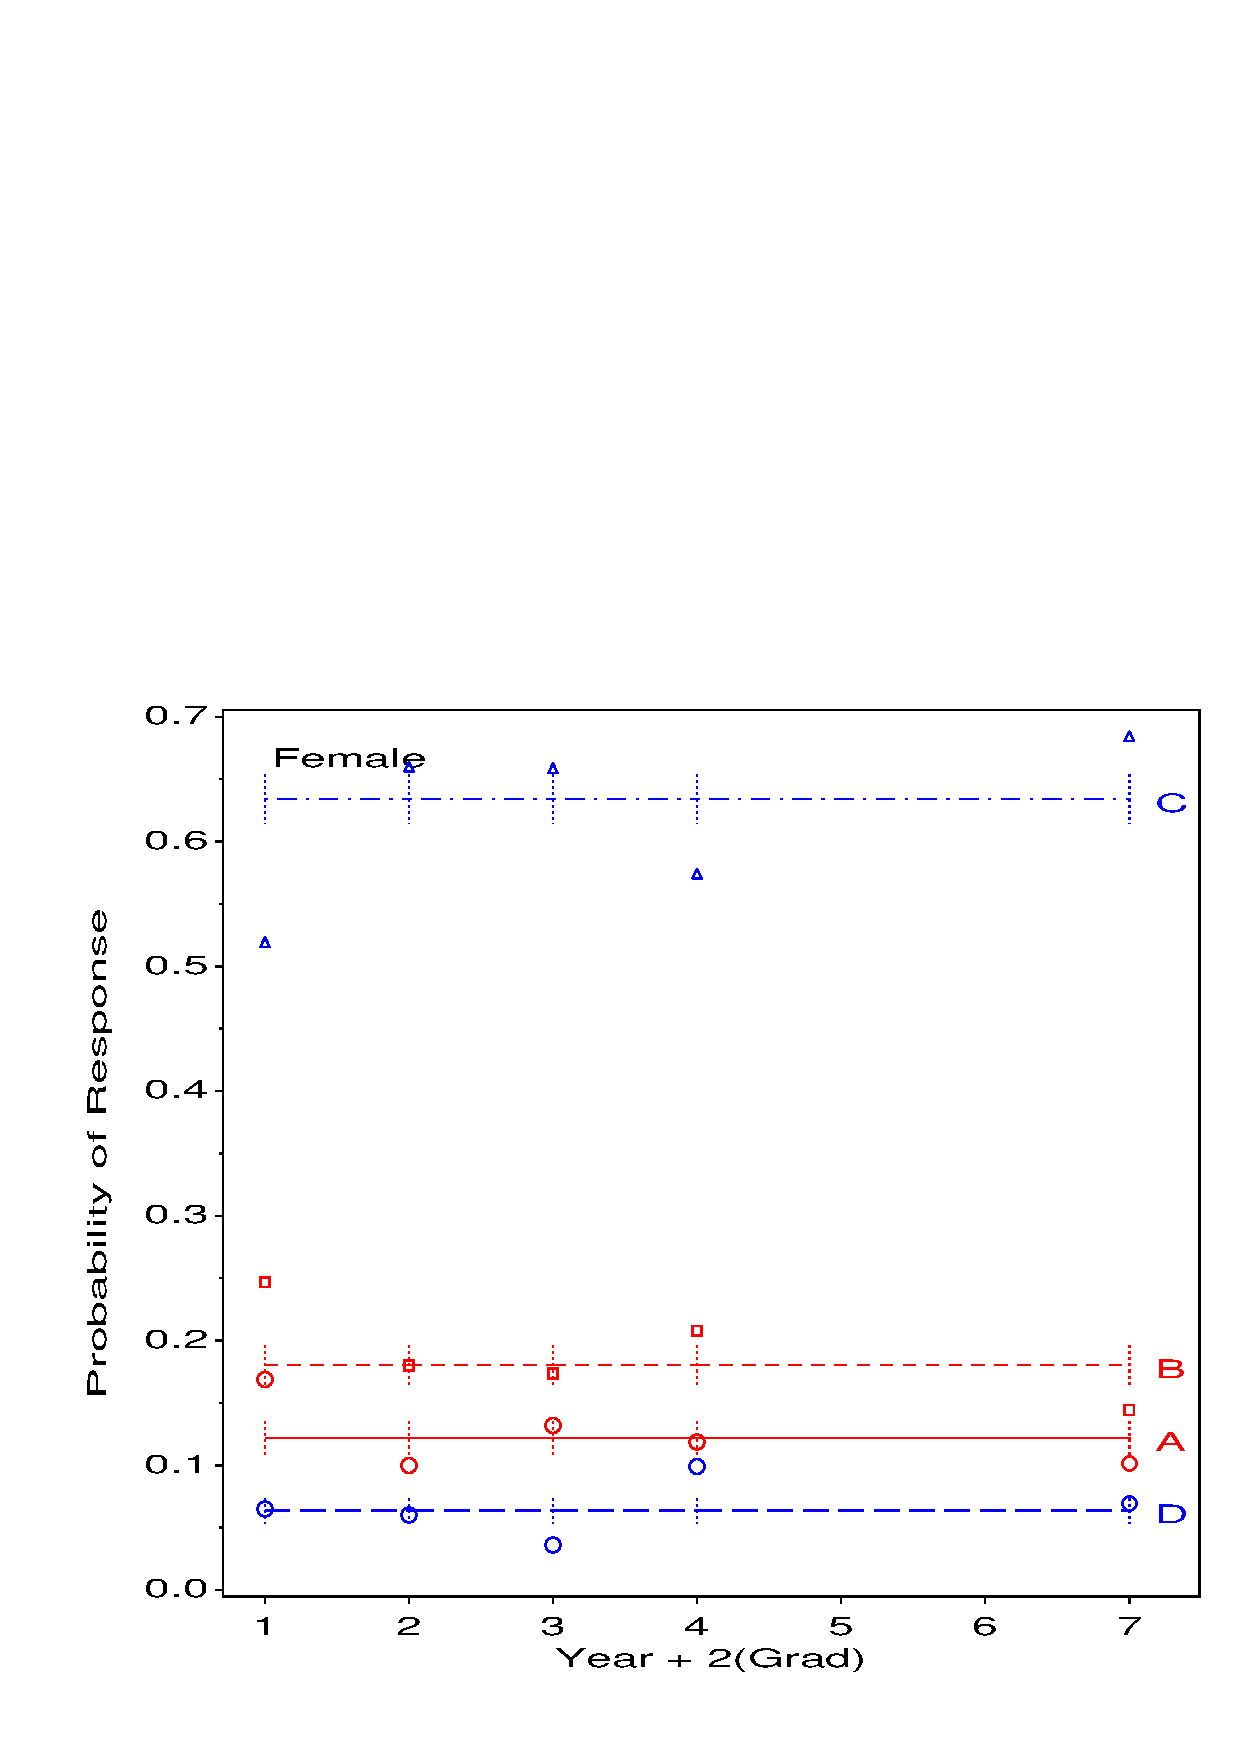
\includegraphics[width=1\linewidth]{vietnam31}
 \end{minipage}%
 \hfill
 \begin{minipage}[t]{.49\linewidth}
  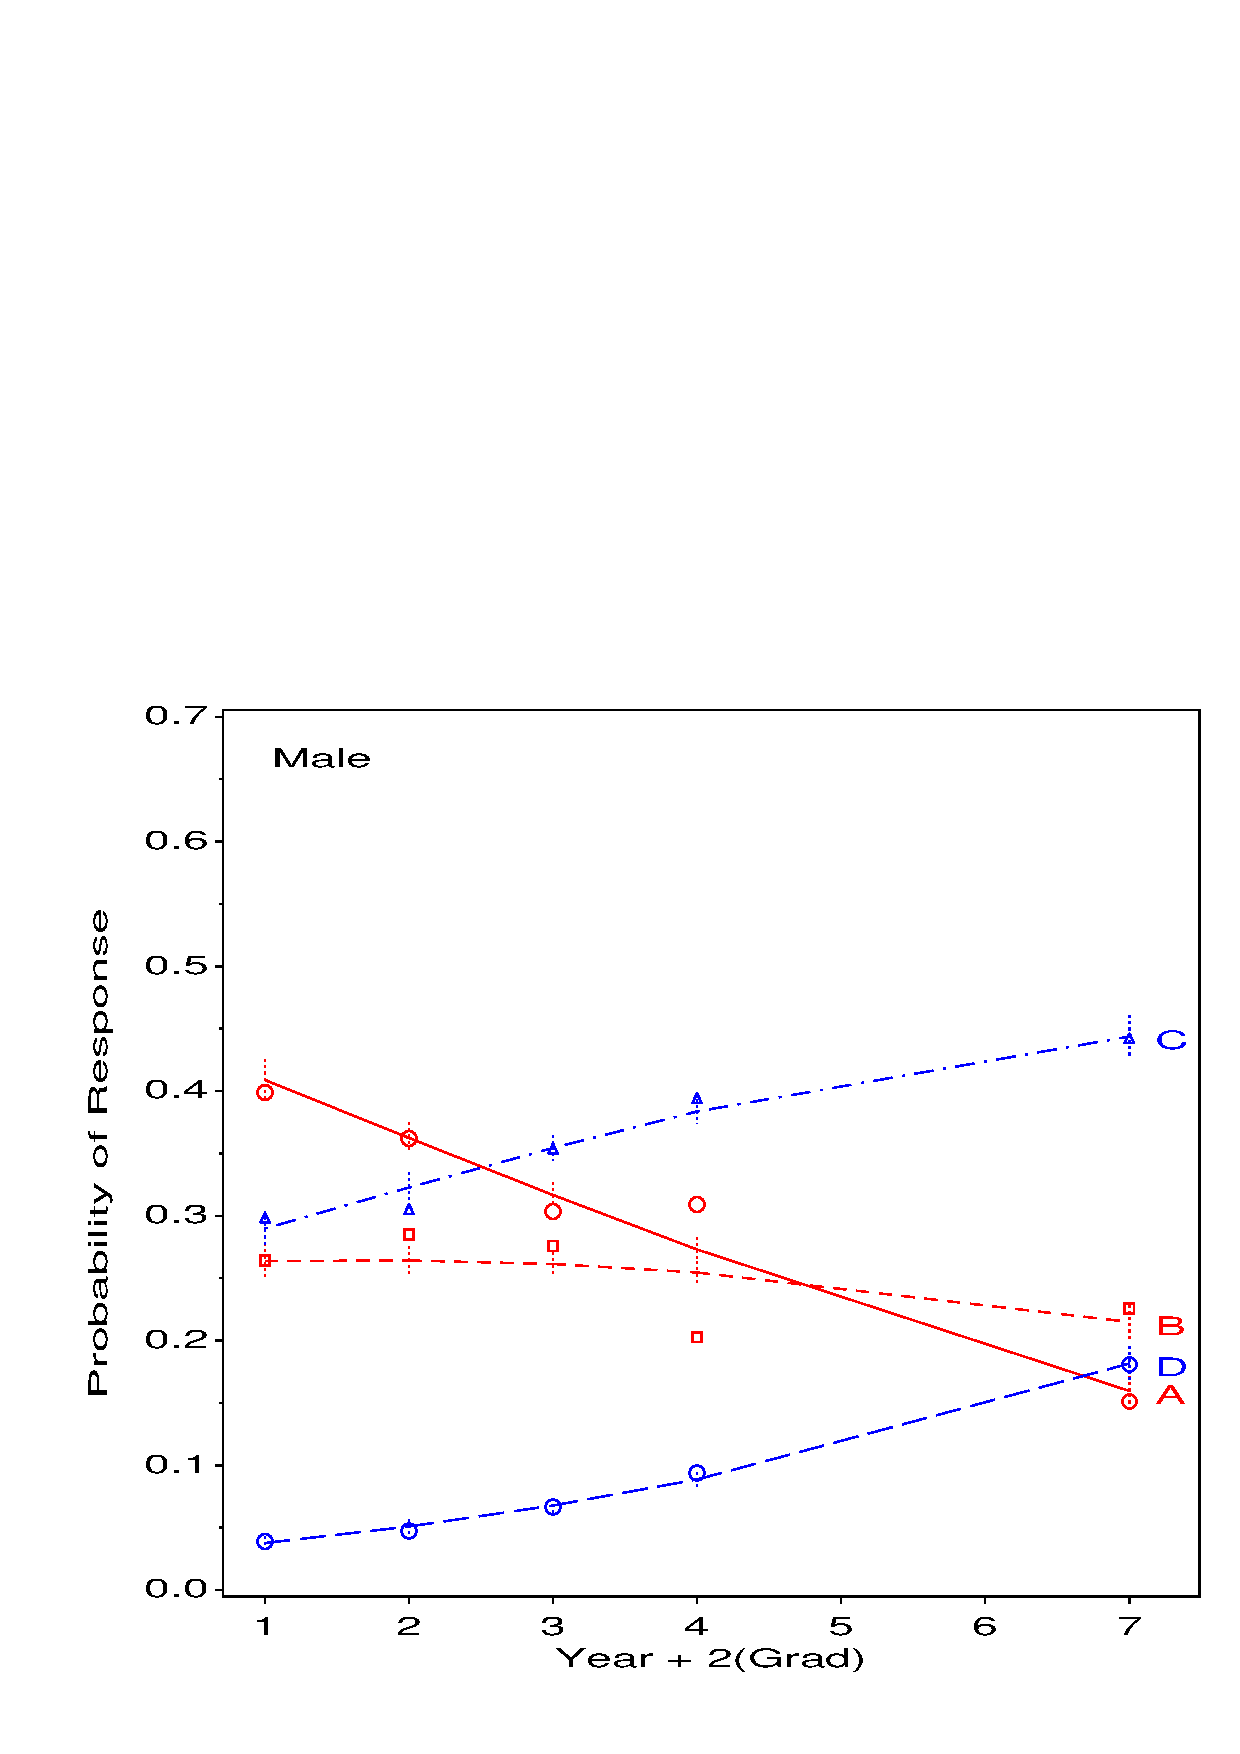
\includegraphics[width=1\linewidth]{vietnam32}
 \end{minipage}
 \caption{Observed and fitted probabilities for model $R = S + Y_{lin}(M)$, Graduate students=7}\label{fig:vietnam3}
\end{figure}

This model fits quite well overall, but there are still several
discrepant points.
We examine residuals and influence diagnostics for this model in
the following section
(\exref{ex:vietnam3}).
\end{Example}


%% two subfig side-by-side
\begin{figure}[htb]
 \begin{minipage}[t]{.49\linewidth}
  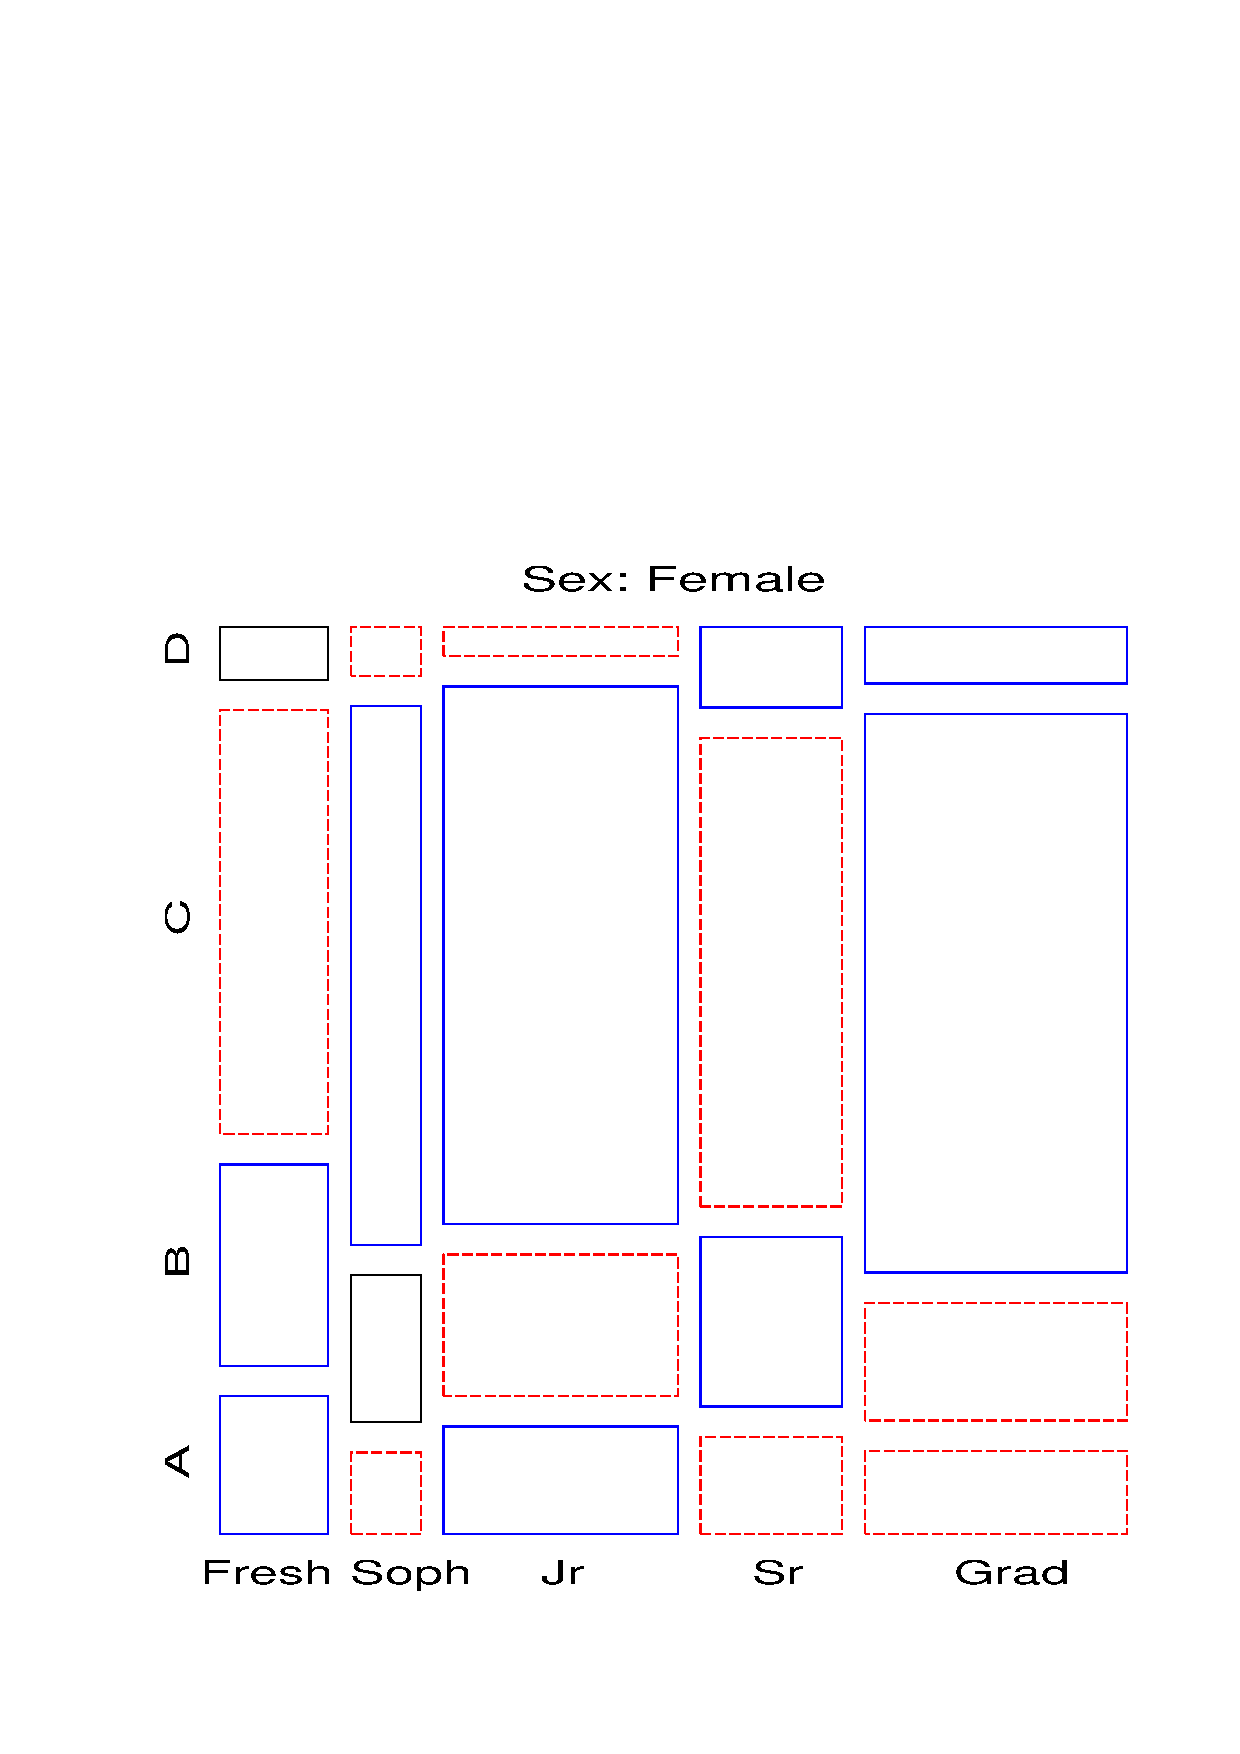
\includegraphics[width=1\linewidth,clip]{mosviet1}
 \end{minipage}%
 \hfill
 \begin{minipage}[t]{.49\linewidth}
  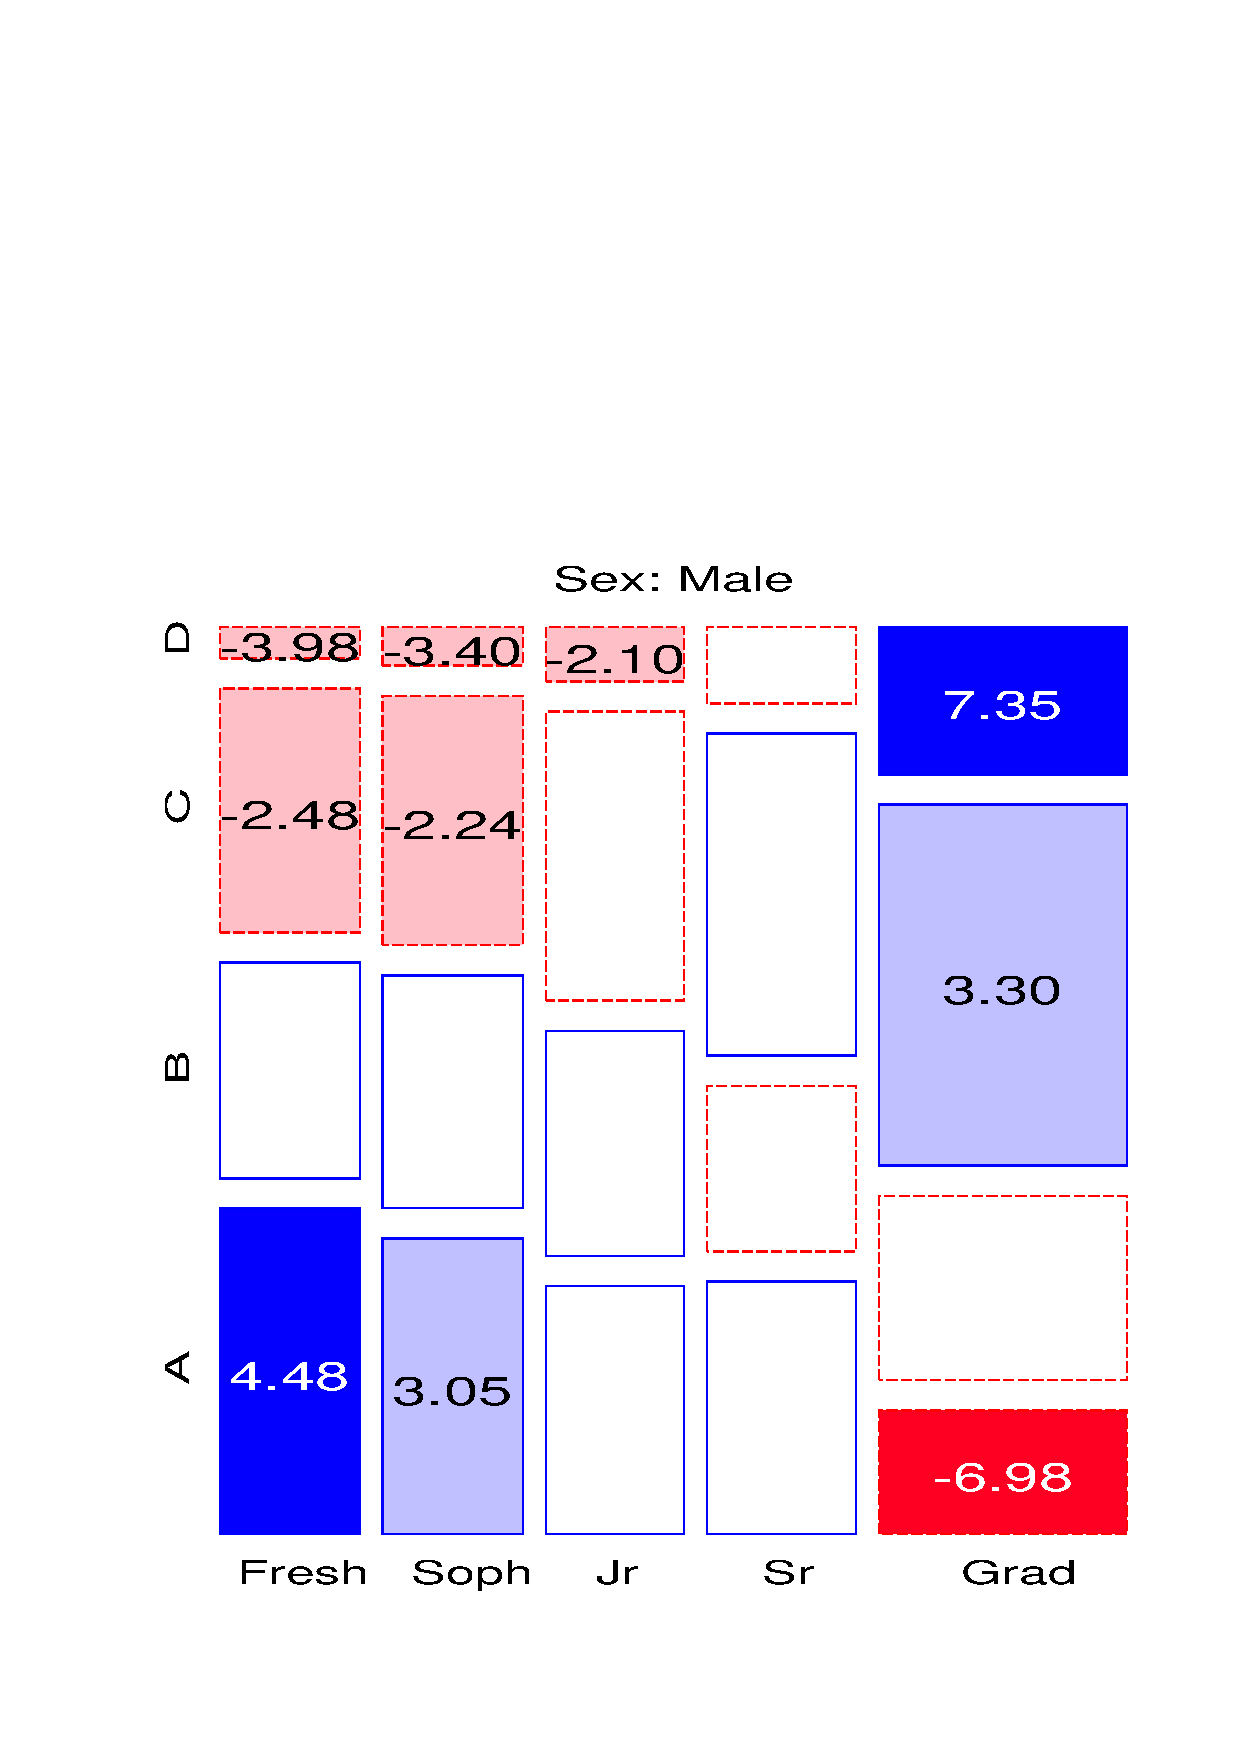
\includegraphics[width=1\linewidth,clip]{mosviet2}
 \end{minipage}
 \caption{Partial mosaic plots, by sex, for Vietnam war data}\label{fig:mosviet}
\end{figure}
With the variables in each mosaic ordered Year, Response,
recall that the height of each bar shows the (conditional) proportion
of students in each year who chose each response. There is no systematic
pattern for women, but the pattern of heights of the boxes, and of the
residuals from independence for men is very systematic.
The trend over years is easiest to see for responses A and D;
note that there is a large jump in proportion choosing these responses
between 4th year students and graduate students.
Perhaps our assumption of a linear trend with year for males needs
adjustment.

A \CA\ plot also displays residuals from a background model.  Here
we choose the null-response model of joint independence, $[SY] [R]$, so that all associations
between the response and the sex-year combinations will be shown.
To do this, we first transpose the data so that the responses
are columns and the sex-year populations are rows.
\begin{listing}
%include catdata(vietnam);

*-- Reshape to two-way table, SexYr x Response;
proc transpose data=vietnam prefix=R out=viet2way;
   var count;
   by sex year;

data viet2way;
   set viet2way;
   rename r1=A r2=B r3=C r4=D;
   sexyr = sex || put(year,1.);
   drop _name_;
proc print;

%corresp(data=viet2way, var=A--D, id=sexyr, interp=none join);
\end{listing}

The plot, shown in \figref{fig:vietcores} is quite revealing.
The response points, A--D
largely define the first dimension,
which accounts for 73.6\% of the association from the null-response model.
The year points for men, M1--M5,
are also ordered along this dimension, but male graduate students are far
from the male undergraduates.
The year points for women are tightly clustered, and aligned closest to
response C, their most preferred alternative.
The second dimension seems largely to do with the contrast between the relatively high choice for response D (``immediate withdrawal'')
among male graduate students and general preference for response C
(``de-escalate'') among most women.

%% one figure
\begin{figure}[htb]
  \centering
  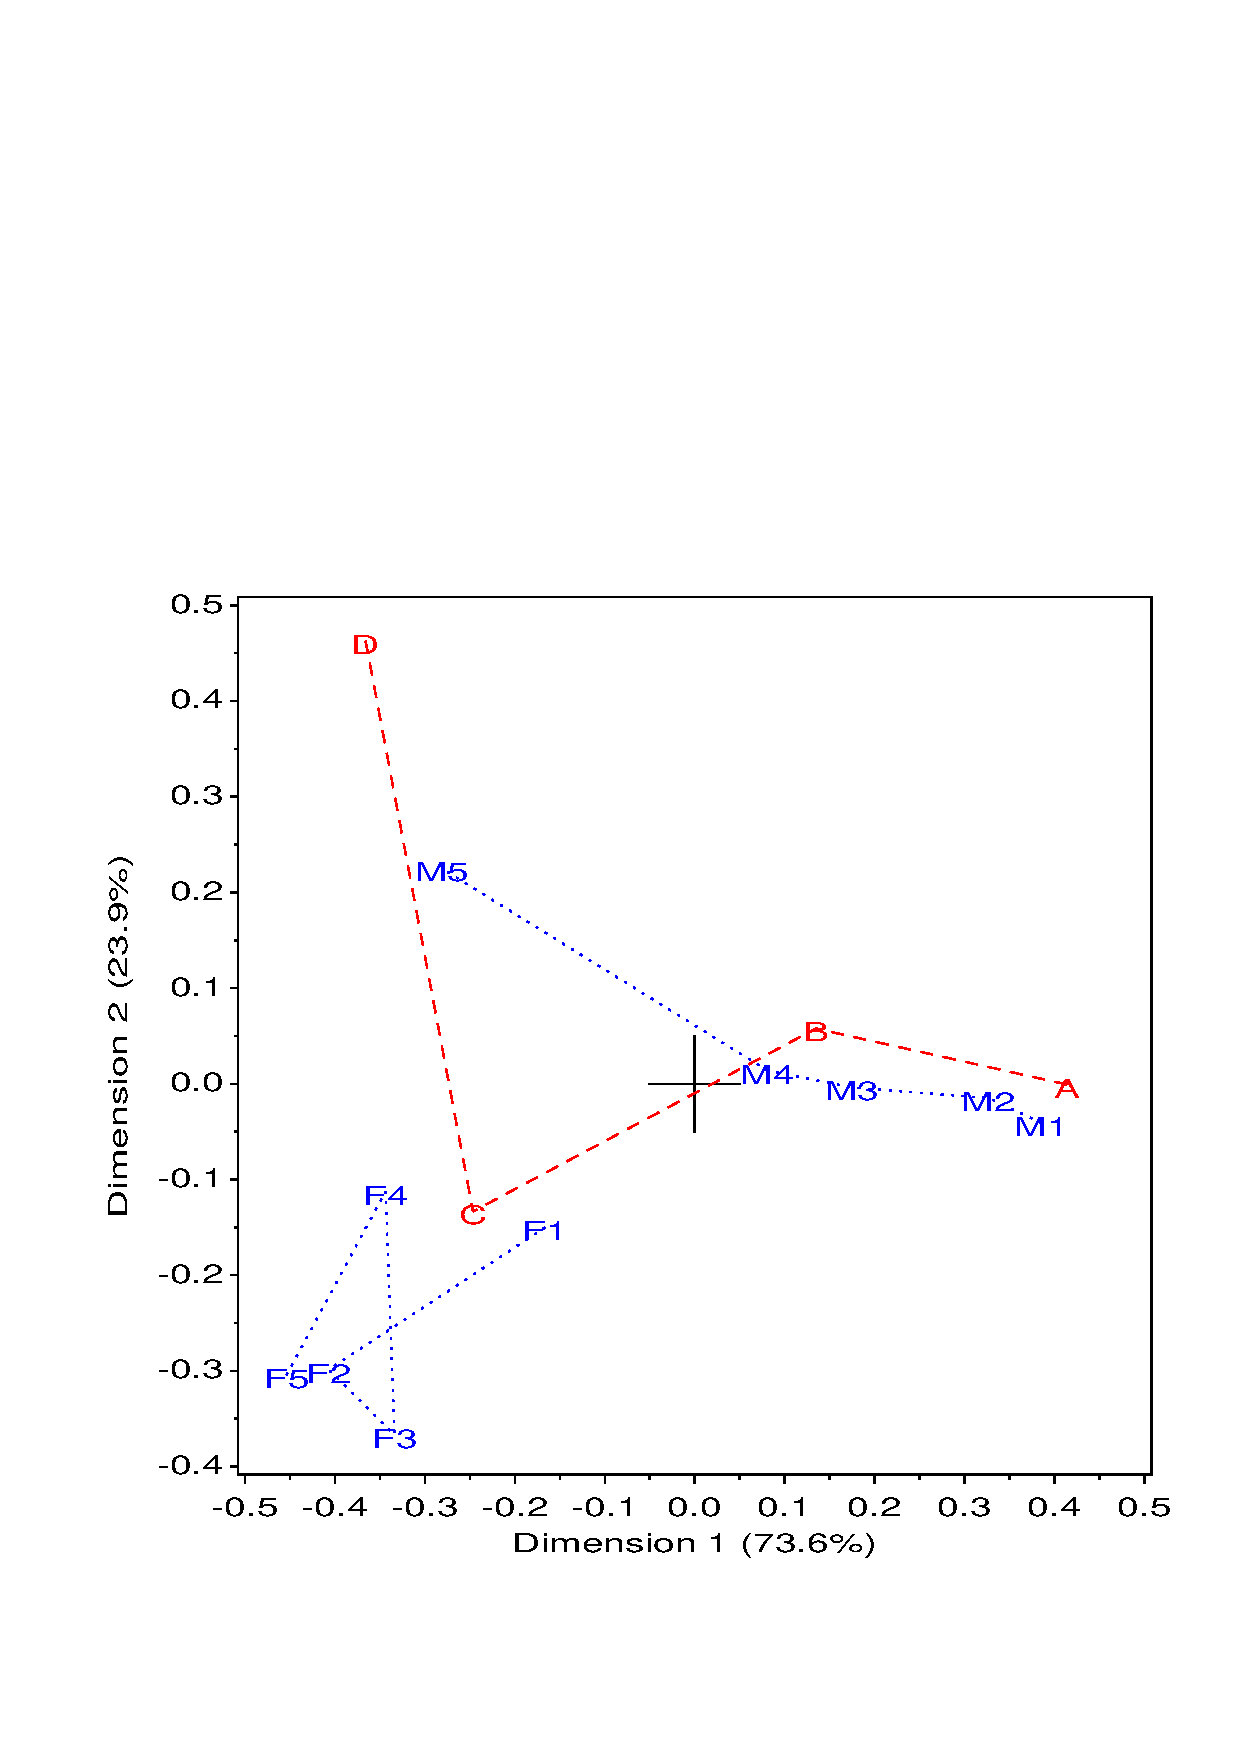
\includegraphics[scale=.6,clip]{vietcores}
  \caption{Correspondence analysis display for model $[SY][R]$}%
  \label{fig:vietcores}
\end{figure}

Both \figref{fig:mosviet} and \figref{fig:vietcores} indicate that our
assumption of linear spacing of year for men is incorrect, particularly
for graduate students.
A simple approach is to replace the variable \pname{year} with a new
variable, \pname{YR}, for which graduate students are some number
greater than 5.
Varying the year for graduate students over the range 5--10 gives
the residual \GSQ\ values (with 21 df)
in \tabref{tab:vietgrad}, and suggests that
7 years for graduate students gives the best fit.  The plot
of fitted and observed values under the revised model is shown in \figref{fig:vietnam3}.
\begin{Example}[vietnam3]{Student opinion about the Vietnam war}
The revised model, with linear effects of year on each logit,
and with graduate students treated as \pname{yr=7}
 shown in \figref{fig:vietnam3} was fit using
\PROC{CATMOD}.  However, influence diagnostics are
easier to obtain using
\PROC{GENMOD}.
The same model can be fit using \PROC{GENMOD} by defining a dummy variable
for women and an interaction between \pname{yr} and a dummy variable
for men.
\begin{listing}
data vietnam;
   set vietnam;
   yr = year + 2*(year=5);
   mlin =  yr * (sex='M');
   female = (sex='F');
   cell = trim(sex)|| put(year,1.)|| trim(put(response,letter.));
   label yr="Year + 2(Grad)";

proc genmod data=vietnam;
   class year sex response;
   model count = year|sex response|mlin  response|female /
         dist=poisson obstats residuals;
   make 'obstats' out=obstats;
\end{listing}
Normally, one would need to merge the input \Dset\ with the \pname{obstats},
and calculate hat values, Cook's D or other quantities for plotting:
\begin{listing}
%let k=8;
data obstats;
   merge vietnam obstats;
   h = hesswgt * std**2;
   cookd = streschi**2 * h/((1-h) * &k);
\end{listing}
where \pname{k=8} is the number of estimated parameters.

Instead, the \macro{INFLGLIM} (\macref{mac:inflglim}) automates these steps, and
gives various influence plots of residuals from a given
model.  The macro plots all combinations of the variables given
by the \mparm{GY}{INFLGLIM} against the variables given by the \mparm{GX}{INFLGLIM},
using a bubble symbol whose size is proportional to the
\mparm{BUBBLE}{INFLGLIM}, usually Cook's D.

Here, we plot the one-step estimates of change in deviance
($\Delta G_{(-i)}^2$, or \pname{DIFDEV})
due to deleting each cell against hat values,
using bubble symbols with area proportional to Cook's D.
The \mparm{infl}{INFLGLIM} determines the criterion for labeling
potentially influential points.
\begin{listing}
%inflglim(data=vietnam, resp=count,
    class=year sex response,
    model= year|sex  response|mlin  response|female,
    dist=poisson, id=cell,
    infl=%str(difdev>4 or &bubble>1 or hat>1.5*&hcrit),
    gy=difdev, gx=hat, bubble=cookd);
\end{listing}

This plot (\figref{fig:vietgen3}) shows that there are still two
large residuals: 4th year men choose response B substantially less often
than predicted (accounting for over one-third of the model deviance), and first year women choose response C less than
predicted.
%% one figure
\begin{figure}[htb]
  \centering
  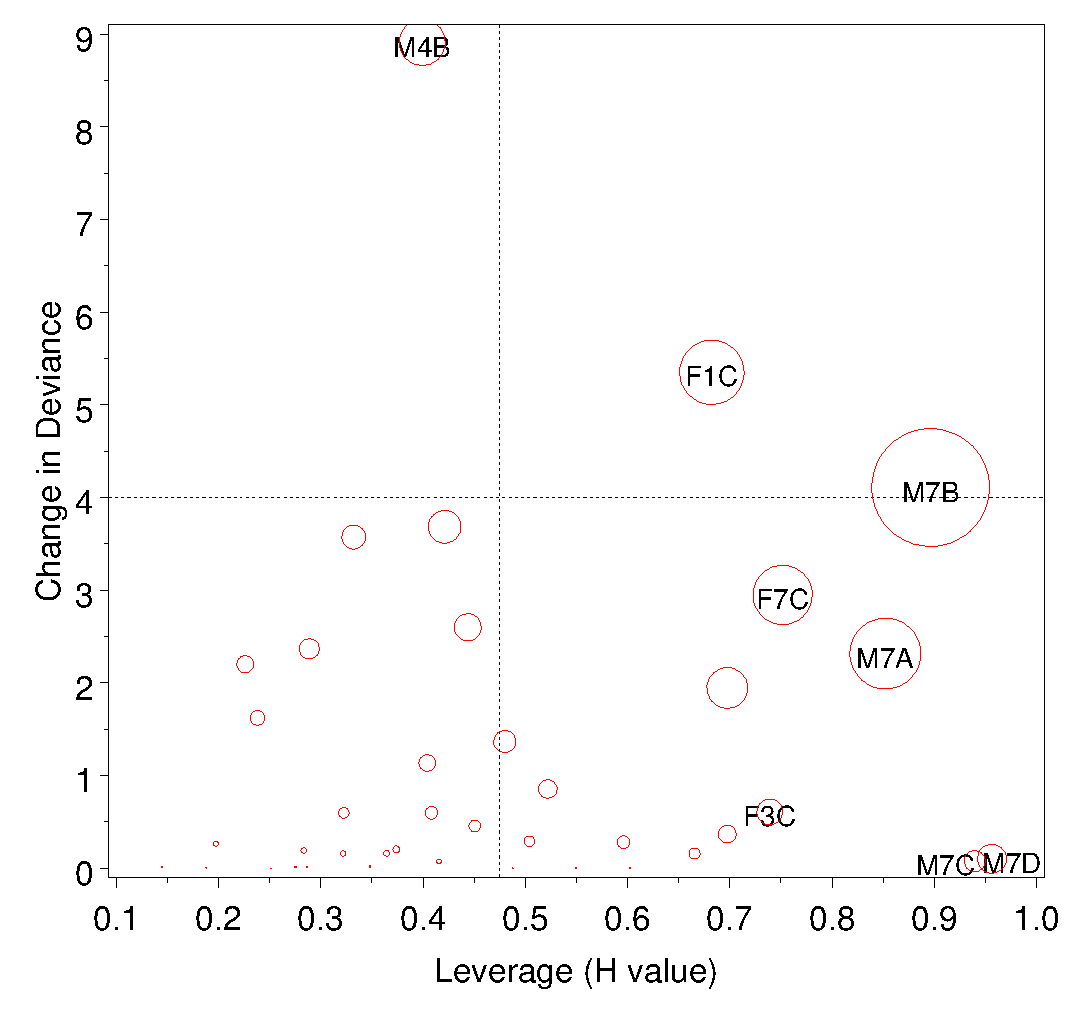
\includegraphics[scale=.6]{vietgen3}
  \caption{Influence plot for model $R = S + Y_{lin}(M)$, Graduate students=7}%
  \label{fig:vietgen3}
\end{figure}
We complete the analysis and this example with a half-normal plot of
these residuals, shown in \figref{fig:vietgen4}.  Although there is
evidence of non-normality in the distribution of residuals,  even the largest
values are within the simulated envelope.
\begin{listing}
%halfnorm(data=vietnam, resp=count,
   class=sex year response,
   model=year|sex  response|mlin  response|female,
   dist=poisson, id=cell);
\end{listing}

\begin{figure}[htb]
  \centering
  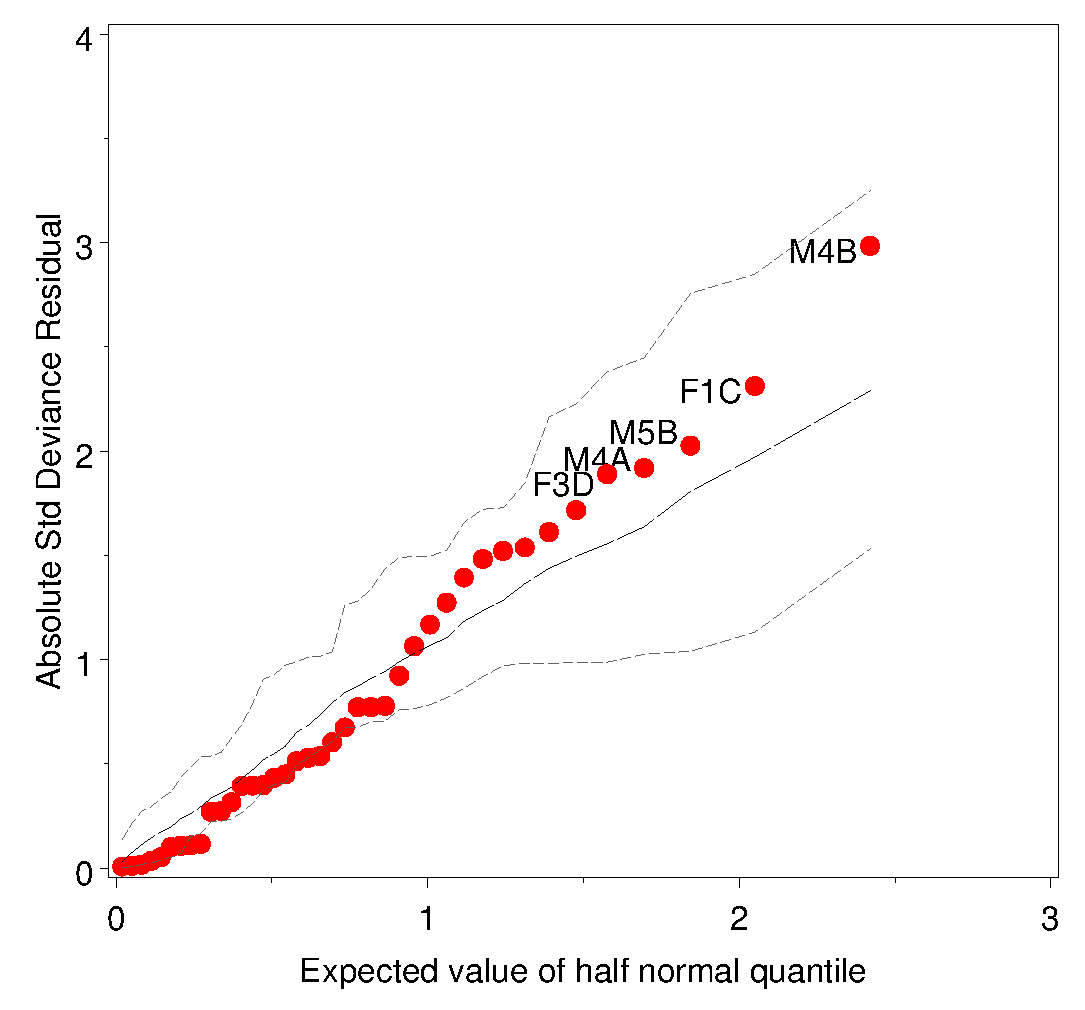
\includegraphics[scale=.6]{vietgen4}
  \caption{Half-normal plot for model $R = S + Y_{lin}(M)$, Graduate students=7}%
  \label{fig:vietgen4}
\end{figure}
\end{Example}

\begin{table}[htb]
 \caption{Profile deviance analysis of Year for Graduate Students}\label{tab:vietgrad}
 \begin{center}
 \begin{tabular}{cr}
  \hline
  Grad Year & \GSQ (21) \\
  \hline
  5 &  38.10 \\ 
  6 &  26.69 \\ 
  7 &  23.87 \\ 
  8 &  23.99 \\ 
  9 &  25.13 \\ 
  10 & 26.58 \\ 
  \hline
 \end{tabular}
 \end{center}
\end{table}


%% two subfig side-by-side
\begin{figure}[htb]
 \begin{minipage}[t]{.49\linewidth}
  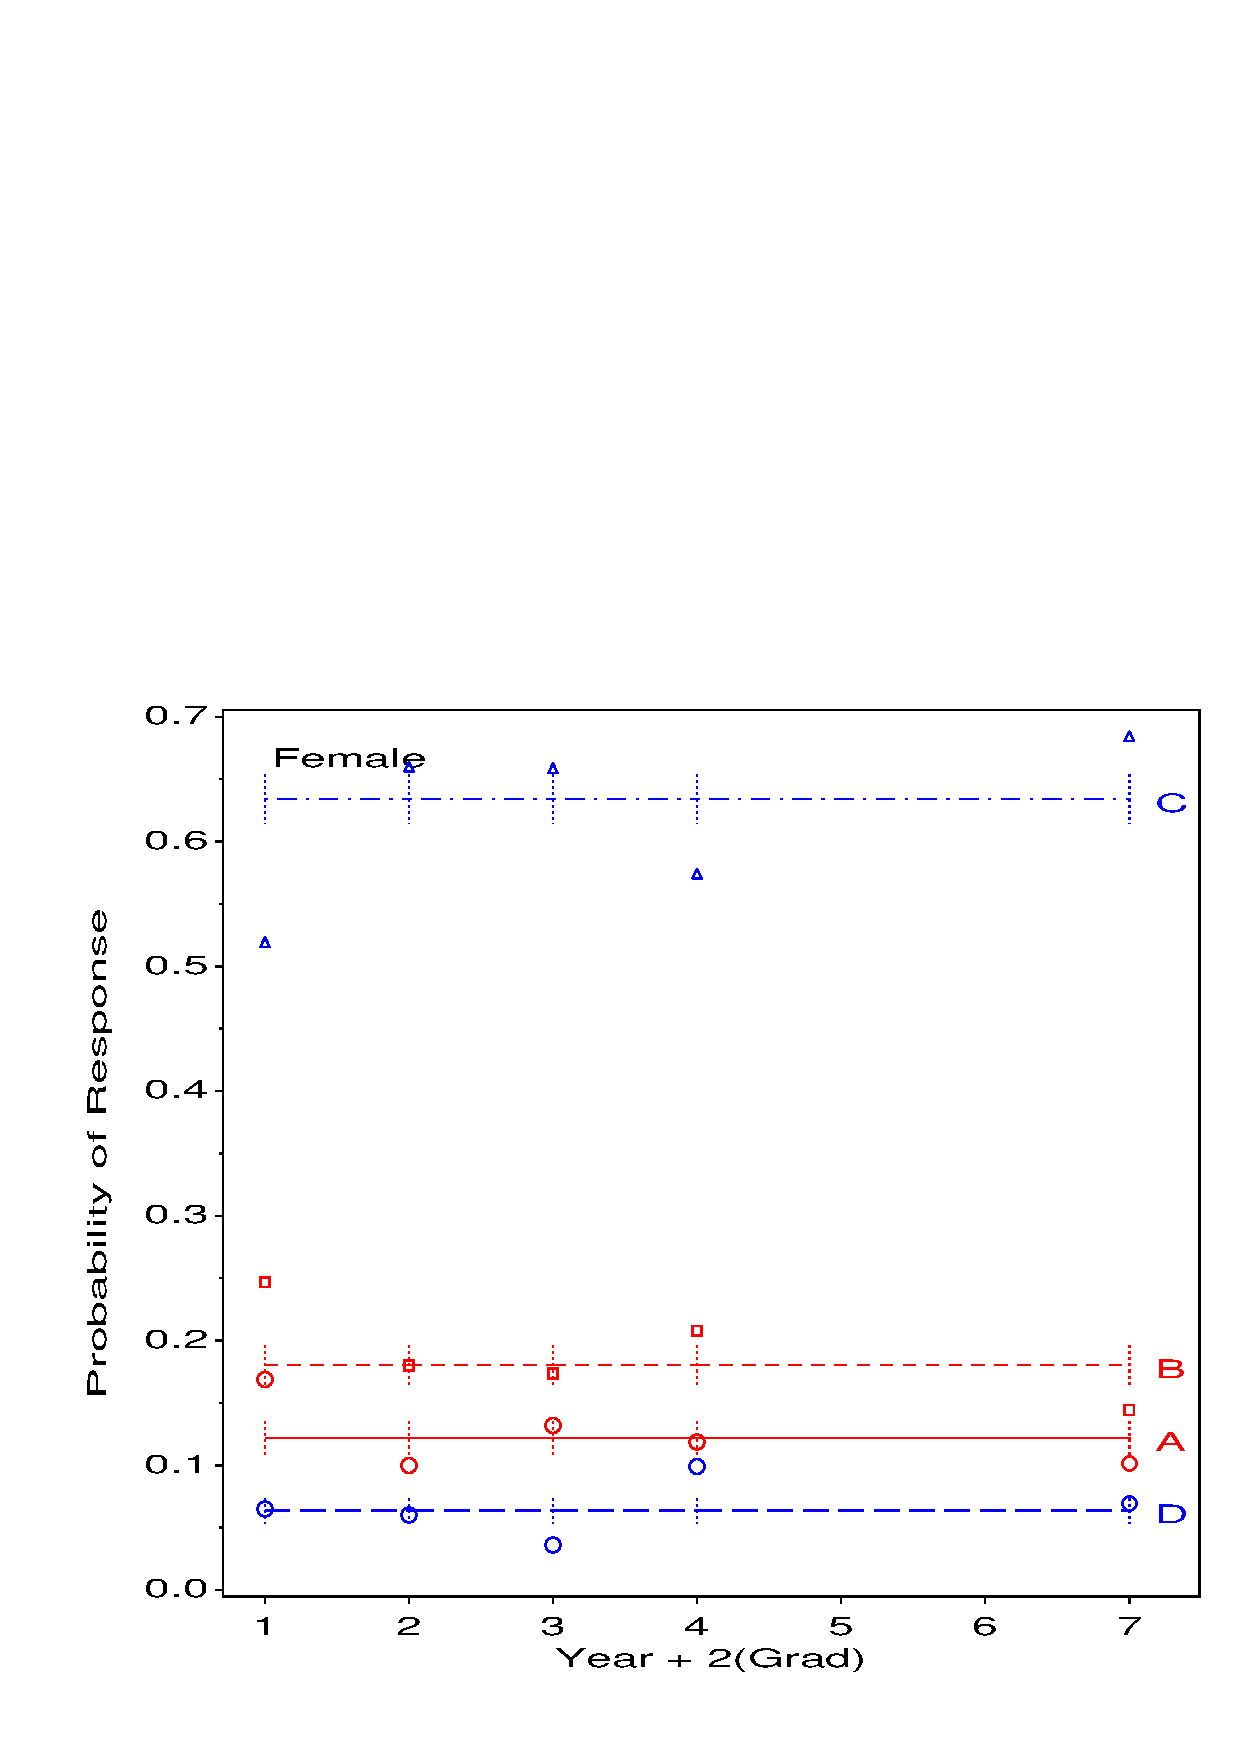
\includegraphics[width=1\linewidth]{vietnam31}
 \end{minipage}%
 \hfill
 \begin{minipage}[t]{.49\linewidth}
  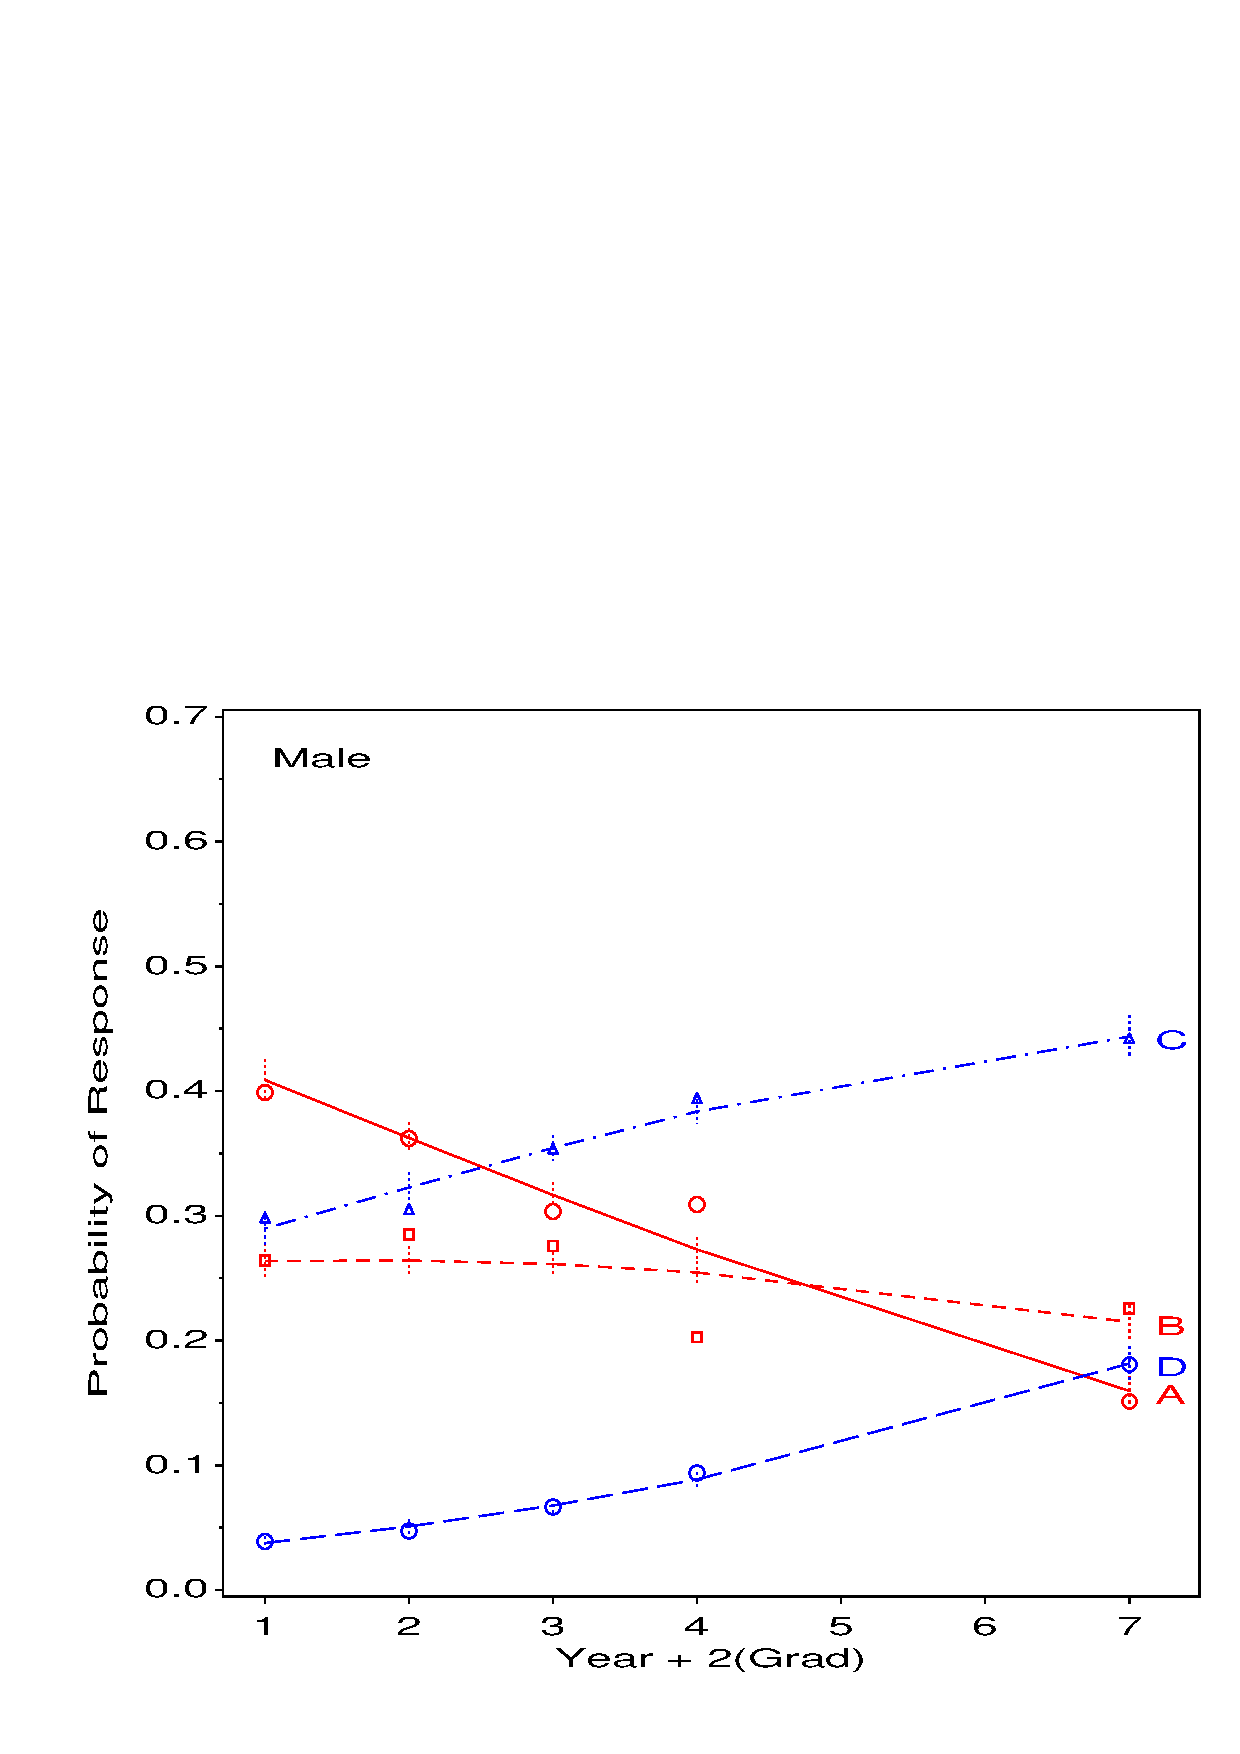
\includegraphics[width=1\linewidth]{vietnam32}
 \end{minipage}
 \caption{Observed and fitted probabilities for model $R = S + Y_{lin}(M)$, Graduate students=7}\label{fig:vietnam3}
\end{figure}

This model fits quite well overall, but there are still several
discrepant points.
We examine residuals and influence diagnostics for this model in
the following section
(\exref{ex:vietnam3}).
\end{Example}

\section{Influence and diagnostic plots}\label{sec:logist-infl}

In ordinary least squares (OLS) regression, measures of \glossterm{influence}
(leverage, Cook's D, DFBETAs, etc.) help you to determine whether
individual cases (or cells in grouped data)
have undue impact on the fitted regression model and
the coefficients of individual predictors.
Analogs of most of these
measures have been suggested for logistic regression.
\citet{Pregibon:81} provided the theoretical basis for these methods,
exploiting the relationship between logistic models and
weighted least squares.  Some
additional problems occur in practical applications to
logistic regression because the response
is discrete, and because the leave-one-out diagnostics are more
difficult to compute.

\subsection{Residuals and leverage}
\ix{logistic regression!residuals|(}
As in ordinary least squares regression, the influence (actual impact)
of an observation in logistic models depends multiplicatively
on its residual (disagreement between $y_i$ and $\hat{y}_i$)
and its leverage (how unusual $\vec{x}_i$ is in the space of the
explanatory variables).
The multiplicative definitions imply that a case is influential to
the extent that it is poorly fit \emph{and} has unusual values of
the predictors.

In logistic regression, the simple raw residual is just $e_i \equiv y_i - \hat{p}_i$,
where $ \hat{p}_i = \exp( \vec{x}_i\trans \vec{b} ) / [1 + \exp( \vec{x}_i\trans \vec{b} )]$.
The  Pearson and deviance residuals are more useful for identifying
poorly fitted observations, and are components of overall goodness-of-fit
statistics.
The \boldital{Pearson residual} is defined as
\begin{equation}\label{eq:reschi}
r_i \equiv \frac{e_i}{\sqrt{ p_i  (1-p_i)}}
\end{equation}
and the Pearson chi-square is therefore $\chisq = \sum r_i^2$.
The \boldital{deviance residual} is
\begin{equation}\label{eq:resdev}
g_i \equiv \pm { -2 [ y_i \log p_i  + (1-y_i) \log (1-p_i) ] }^{1/2}
\end{equation}
where the sign of $g_i$ is the same as that of $e_i$.
Likewise, the sum of squares of the deviance residuals gives
the overall deviance,
$G^2 = -2 \log \mathcal{L}(\vec{b}) = \sum g_i^2$.

When $y_i$ is a binomial count based on $n_i$ trials (grouped data),
the Pearson residuals \eqref{eq:reschi} then become
\begin{equation*}%\label{eq:reschi2}
r_i \equiv \frac{y_i -n_i p_i}{\sqrt{n_i  p_i  (1-p_i)}}
\end{equation*}
with similar modifications made to \eqref{eq:resdev}.
\ix{logistic regression!residuals|)}

\ix{logistic regression!leverage|(}
Leverage measures the \emph{potential} impact of an individual case
on the results, which is directly proportional to how far an
individual case is from the centroid in the space of the
predictors.  Leverage is computed as the diagonal elements,
\(h_{ii}\), of the ``Hat'' matrix, \(\mat{H}\),

\begin{equation*}%\label{eq:}
\mat{H} = {\mat{X}}^\star
{( {\mat{X}^\star}\trans {\mat{X}}^\star )}^{-1} {\mat{X}^\star}\trans
\end{equation*}
where \({\mat{X}} ^\star = {\mat{V}}^{1/2} \mat{X}\), and \(\mat{V}  =
\diag [ \hat{\vec{p}} ( 1 - \hat{\vec{p}})] \).  As in OLS,
leverage values are between 0 and 1, and a leverage value,
\(h_{ii}  > 2 (k+1) /  n\) is considered ``large''; here, \(k\) is the
number of predictors, and \(n\) is the number of cases.
In OLS, however, the hat values depend only on the $X$s, whereas
in logistic regression, they also depend on the dependent
variable values and the fitted probabilities (through $\mat{V}$).
As a result, an observation may be extremely unusual on the predictors,
yet not have a large hat value, if the fitted probability is near 0 or 1.
\ix{logistic regression!leverage|)}

\subsection{Influence diagnostics}\label{sec:logist-infldiag}
\ix{logistic regression!influence diagnostics|(}
Influence measures assess the effect that deleting an
observation has on the regression parameters, fitted values, or the
goodness-of-fit statistics.  In OLS, these measures
can be computed exactly from a single regression.
In logistic regression, the exact effect of deletion
requires refitting the model with each observation deleted in turn
(because the estimating equations \eqref{eq:like4} are nonlinear),
a time-intensive computation.
Consequently, \citet{Pregibon:81} showed how analogous deletion
diagnostics may be approximated by performing one additional step
of the iterative procedure.

The simplest measure of influence of observation $i$ is the standardized change in the coefficient for each variable due to omitting that observation,
termed \boldital{DFBETA}s.  From the relation \citep[p. 716]{Pregibon:81}
\begin{equation*}%\label{eq:dfbetas}
 \vec{b} -  \vec{b}_{(-i)} = (\mat{X}\trans \mat{V} \mat{X})^{-1} \vec{x}_i (y_i - p_i) / (1 - h_{ii})
 \comma
\end{equation*}
the estimated standardized change in the coefficient for variable $j$ is
\begin{equation}\label{eq:dfbeta}
 \mbox{DFBETA}i_j \equiv \frac{b_{(-i)j} -  b_j } {\hat{\sigma} (b_j)}
 \comma
\end{equation}
where $\hat{\sigma} (b_j)$ is the estimated standard error of $b_j$.
With $k$ regressors, there are $k+1$ sets of DFBETAs, which makes their examination burdensome.
Graphical displays ease this burden, as do various summary measures
considered below.

The overall influence of observation $i$ on the estimated regression
coefficients is assessed by analogs of \glossterm{Cook's distance}, which measure
the difference between $\vec{b}$ for all the data and
$\vec{b}_{(-i)}$ estimated without observation $i$.
One measure, $C_i$, is defined as
\begin{equation*}%\label{eq:cookd1}
C_i \equiv ( \vec{b} - \vec{b}_{(-i)} )\trans \:
    \mat{X}\trans \mat{V} \mat{X} \:
     ( \vec{b} - \vec{b}_{(-i)} )
	  \comma
\end{equation*}
and calculated as
\begin{equation}\label{eq:cookd2}
 C_i = \frac{r_i^2 h_{ii}} {(1-h_{ii} )^2}
 \period
\end{equation}
A second measure, $\overline{C}_i$, is calculated as
\begin{equation}\label{eq:cookd3}
 \overline{C}_i = \frac{r_i^2 h_{ii}} {(1-h_{ii} )} = (1-h_{ii} ) C_i
 \period
\end{equation}
Because $0 \le h_{ii} \le 1$, $\overline{C}_i$ will never be larger than $C_i$.
These measures are referred to by the keywords \pname{C} and
\pname{CBAR}, respectively, on the \stmt{OUTPUT}{LOGISTIC}.
Both can be interpreted as squared measures of the change in
size of the confidence intervals for all regression coefficients.
Rules of thumb for noticeably large values are necessarily only
rough indicators, but \citet{Johnson:85} suggests comparing $k C_i$
to a $\chi^2 (k)$ distribution.

The Pearson and deviance residuals defined above do not have equal
variance, but rather have variance $\approx 1-h_{ii}$.  Studentized versions
of both which do have equal variance
are obtained by dividing by $\sqrt{1-h_{ii}}$.  For example, the
studentized deviance residual (\pname{RESDEV}) is $g_i^\star = g_i /
\sqrt{1-h_{ii}}$.
These are most usefully expressed in squared form as the approximate decrease in the
deviance (\pname{DIFDEV}) and Pearson (\pname{DIFCHISQ}) \chisq\ 
associated with deleting observation $i$:
\begin{equation*}%\label{eq:difdev}
  \Delta G_{(-i)}^2 = \frac{g_i^2}{1-h_{ii}}
  \comma
\end{equation*}
and
\begin{equation*}%\label{eq:chi}
  \Delta \chi_{(-i)}^2 = \frac{r_i^2}{1-h_{ii}}
  \period
\end{equation*}
These are both asymptotically distributed as $\chi^2 (1)$, so a value
exceeding 3.84 (or the rounded value, 4) is worth noticing.
They may also be interpreted as indicating how poorly the current
model fits observation $i$.

As with OLS, influential observations signal something unusual:
extreme (or erroneous) predictor values combined with an ill-predicted
response, e.g., someone who died, but should have survived (according to the
model).  They may also signal that some important (perhaps unmeasured)
predictor--- a lurking variable--- has been omitted from the model \citep{Joiner:81} or expressed
on the wrong scale.

\subsection{Influence output from \PROC{LOGISTIC}}
All the influence statistics are
printed when the \opt{influence}{LOGISTIC} is used on the \stmt{MODEL}{LOGISTIC}.
For example, we get these diagnostics for the arthritis data with:
\begin{listing}
proc logistic data=arthrit ;
   model better = _sex_ _treat_ _age_ / influence;
\end{listing}

This produces many pages of output, of the form in \outref{out:glogist3.1},
shown for two of the many diagnostic measures.
With so much output, it is often difficult
to spot unusual observations.  A more useful option, \pname{IPLOTS},
produces index plots of each of the diagnostic measures against
the observation index, with the goal of showing which observations
stand out from the rest.
It is even more useful, I believe, to plot certain diagnostics
against each other, including reference lines showing the nominal
danger-level for each diagnostic,  because they help to pinpoint
\emph{why} certain observations are influential.
Some examples of these plots are described in the following subsection.

\begin{Output}[htbp]
\caption{Regression diagnostics, printed output (partial) for arthritis data}\label{out:glogist3.1}
\small
\verbatiminput{ch6/out/glogist3.1}
\end{Output}

\subsection{Diagnostic plots of influence measures}
Plots of the change in \(\chi^2\) (\pname{DIFCHISQ} or \pname{DIFDEV}) against
either leverage or predicted probability are particularly useful
for detecting unduly influential cases.
These are discrete analogs of plots recommended for linear models
by \citet{Fox:91} and \citet{Friendly:91}.
The estimated overall
influence of each case on the estimated coefficients ($C_i$ or $\overline{C}_i$)
can be shown in a bubble plot where the plotting symbols are circles
proportional to \pname{C} or \pname{CBAR}.

Such plots are produced by the \macro{INFLOGIS},
described in \macref{mac:inflogis}.  For example, these
statements produce plots of DIFCHISQ against both the 
predicted probability, \pname{PRED} 
(\figref{fig:logi1b1}) and
leverage, \pname{HAT}
(\figref{fig:logi1b2}),
using bubbles whose area is proportional
to C:
%% \input{logist1b} %% level: 2
\begin{listing}
title 'Arthritis treatment data';
title2 'Bubble size: Influence on Coefficients (C)';
goptions htext=1.6;
%include data(arthrit);
%inflogis(data=arthrit,
     y=better,               /* response   */
     x=_sex_ _treat_ age,    /* predictors */
     id=id,                  /* case label */
     gy=DIFCHISQ,            /* graph ordinate  */
     gx=PRED HAT,            /* graph abscissas */
     lcolor=RED, bsize=14
     );
\end{listing}

The printed output from the \macro{INFLOGIS} includes a table
identifying any observation of high leverage \emph{or} high influence.
These observations are also labeled in the graphs.  For
example, case 29 is of high leverage, because she is unusual in terms
of the predictors: a young woman given treatment; however, she is not
influential in the fitted model.  Case 77, is not of high leverage,
but is poorly predicted by the model and has a large contribution to
\chisq.

\begin{output}
CASE BETTER  _SEX_  _TREAT_  AGE   HAT  DIFCHISQ   DIFDEV     C

  1     1      0       1      27   .09    4.5781   3.6953   0.4510
 22     1      0       0      63   .06    4.4603   3.5649   0.2898
 29     0      1       1      23   .14    1.0183   1.4005   0.1679
 30     1      1       0      31   .05    4.7485   3.6573   0.2611
 34     1      1       0      33   .05    4.2955   3.4644   0.2236
 55     0      1       1      58   .03    4.9697   3.6759   0.1602
 77     0      1       1      69   .03    8.4977   4.7122   0.2758
\end{output}

\begin{figure}[!htb]
  \centering
  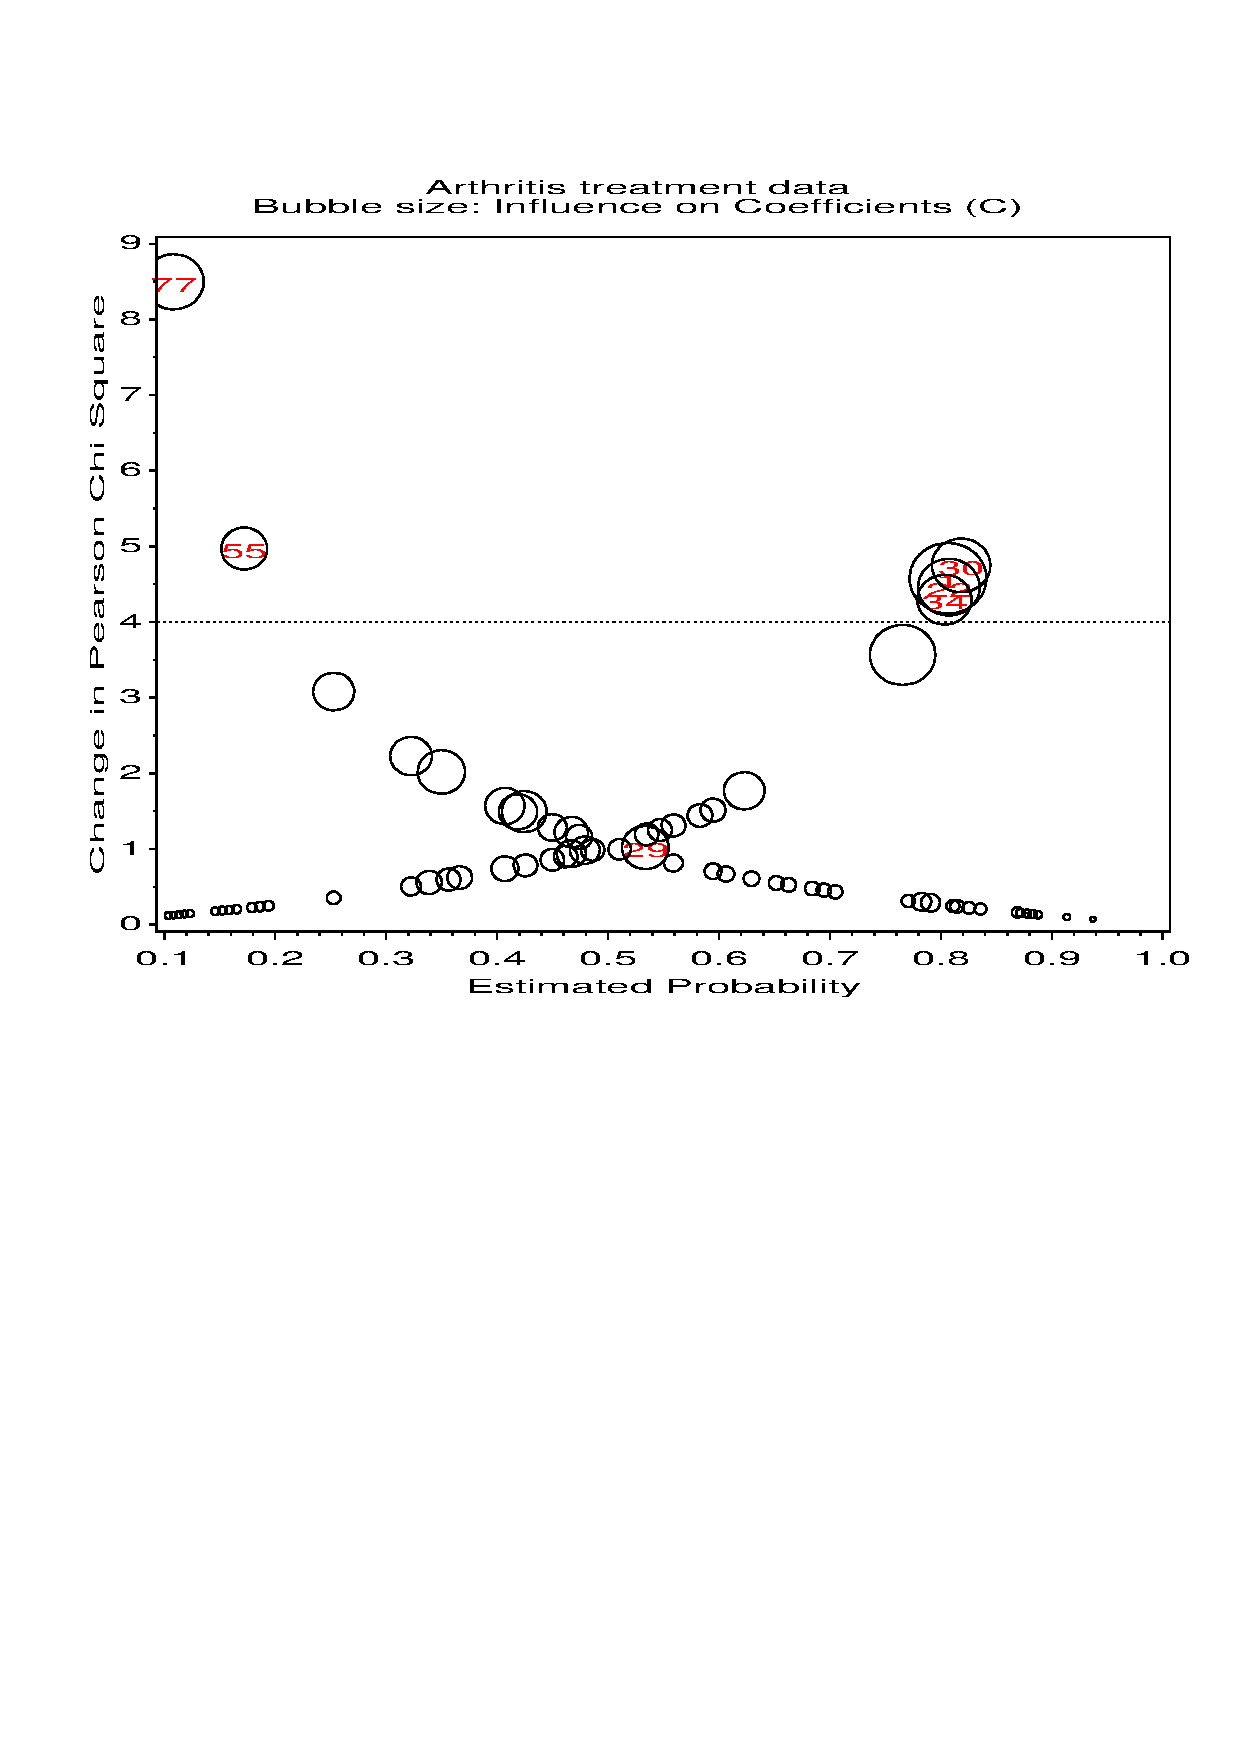
\includegraphics[scale=.7]{ch6/fig/logist1b1}
  \caption[Influence plot for arthritis data]{Influence plot for arthritis data.
Cases with DIFCHISQ \(> 4\) or leverage \(>  (2 k) /  n  = 0.095\) are
labeled as
influential, as indicated by the size of the bubble symbol.
The systematic pattern shown is inherent in the discrete nature of
logistic regression.  The most influential
observations are those with very high or low predicted probabilities.}\label{fig:logi1b1}
\end{figure}

\begin{figure}[!htb]
  \centering
  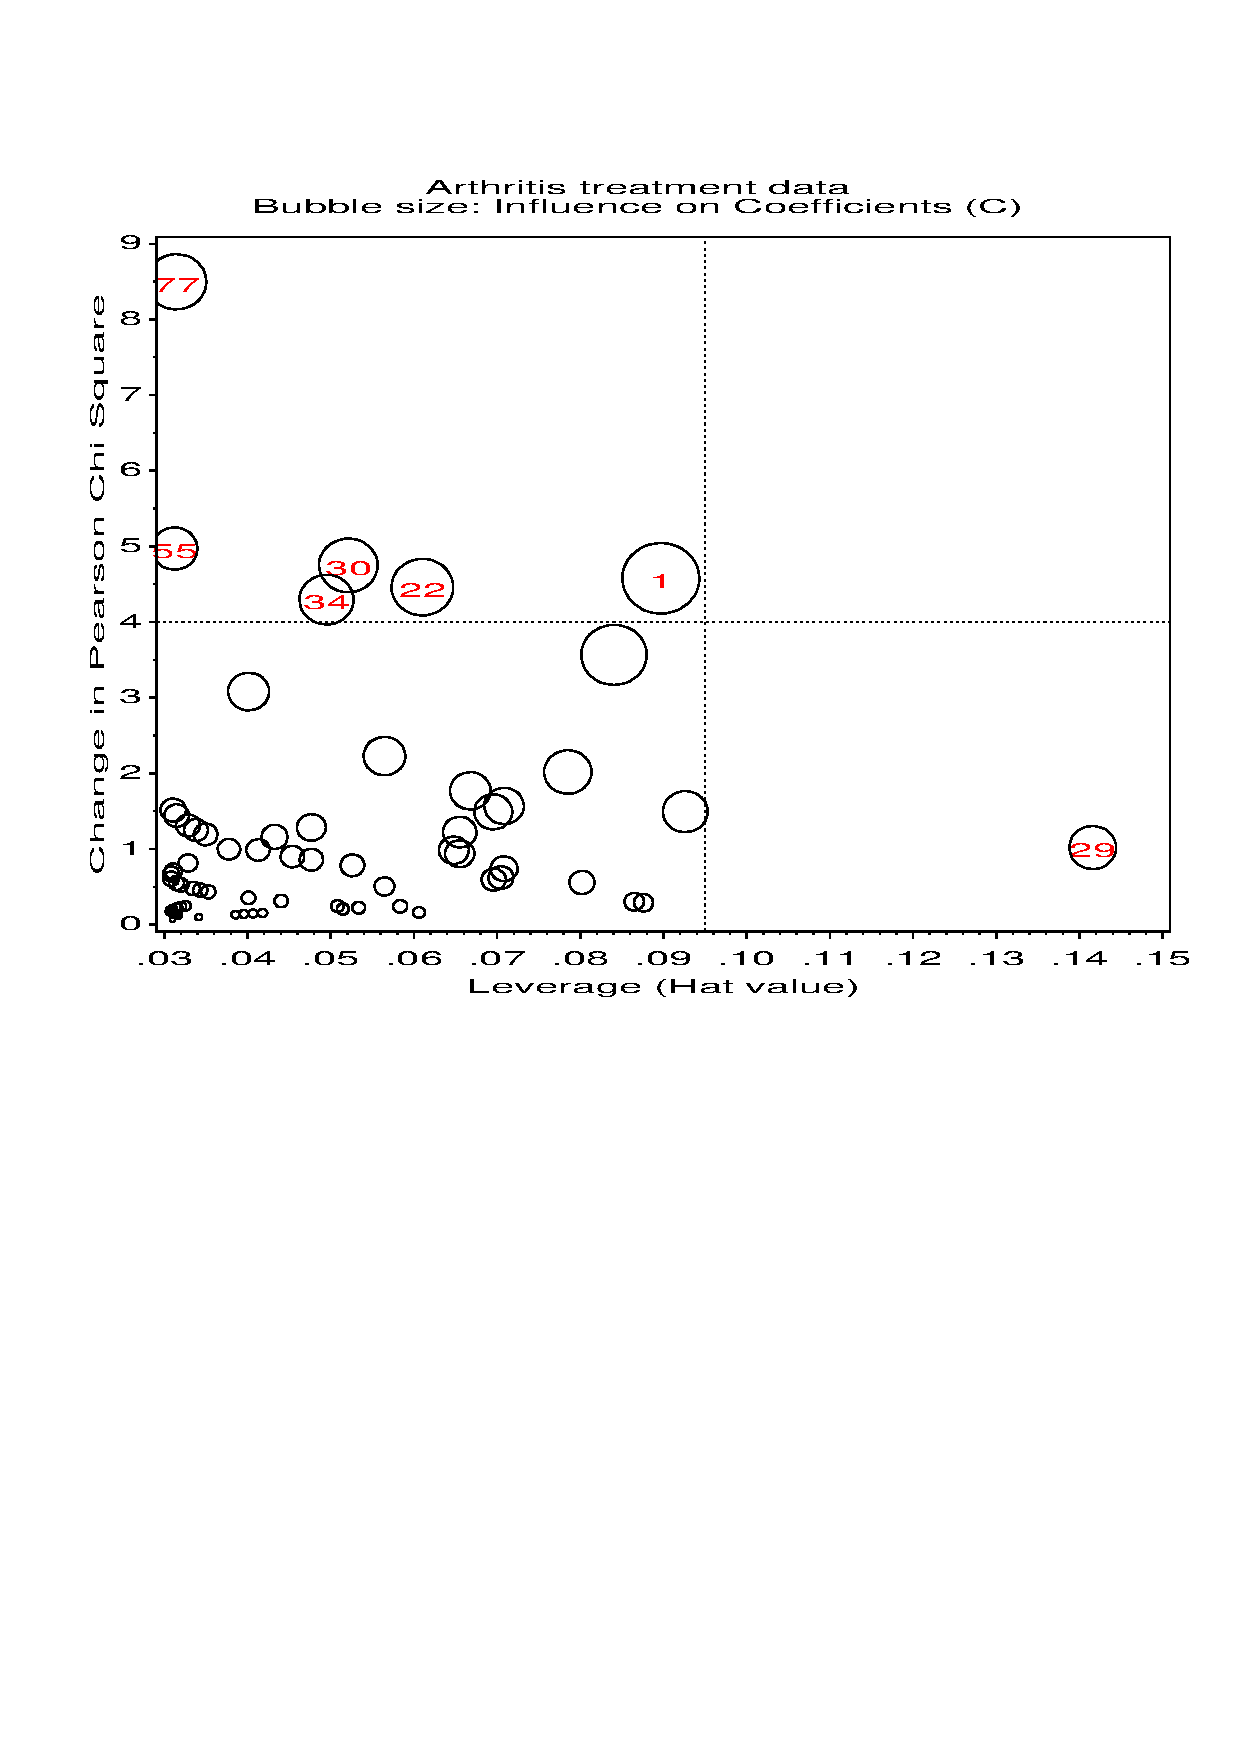
\includegraphics[scale=.7]{ch6/fig/logist1b2}
  \caption[Changes in chi-square vs. leverage]{Changes in chi-square vs.\ leverage.
  The same cases are labeled as in \figref{fig:logi1b1}.
}\label{fig:logi1b2}
\end{figure}
\ix{logistic regression!influence diagnostics|)}

\begin{Example}[icu2]{Survival in the ICU}
The four variable model from \exref{ex:icu1} predicting survival in the ICU
was examined for influential cases with the \macro{INFLOGIS}.
The following macro call produces an influence plot of the \pname{DIFCHISQ}
statistic against hat values, shown in \figref{fig:icu12}.
\begin{listing}
%inflogis(data=icu, y=died, x=age cancer uncons admit,
   id=id,
   gy=difchisq,
   gx=hat);
\end{listing}

%% one figure
\begin{figure}[htb]
  \centering
  \includegraphics[scale=.6]{ch6/fig/icu12}
  \caption[ICU Survival data: Influence plot]{ICU Survival data: Influence plot}%
  \label{fig:icu12}
\end{figure}

Details for the cases identified in the figure are shown in \outref{out:icu1.2}.
None of the cases are particularly influential on the model coefficients overall:
the largest $C_i$ is only 1.04.
Case 208, with the largest hat value, is unusual on the predictors
in this sample: a 70 year old man without cancer, admitted on an elective
basis (who nonetheless died).
On the other hand, case 881, an 89 year old male, admitted unconscious
as an emergency case is poorly predicted because he survived.
Similarly, two other cases (127, 380) with large $\Delta \chi_{(-i)}^2$
are poorly predicted because they died, although they were
young, did not have cancer, and conscious at admission.
From this evidence we might conclude that none of these cases greatly affects the model, its coefficients,
or interpretation.
\begin{Output}[htb]
\caption{ICU data: Influential cases}\label{out:icu1.2}
\small
\verbatiminput{ch6/out/icu1.2}
\end{Output}

That conclusion might not be warranted without further study, particularly
in terms of influence on individual coefficients.
The DFBETAs \eqref{eq:dfbeta} may be obtained in an \ODS\ as shown below:
\begin{listing}
proc logistic data=icu;
   model died = age admit cancer uncons;
   output out=stats dfbetas=dbint dbage dbadmit dbcancer dbuncons ;
\end{listing}

%% two subfig side-by-side
\begin{figure}[htb]
 \begin{minipage}[t]{.49\linewidth}
  \includegraphics[width=1\linewidth,clip]{ch6/fig/icu4b1}
 \end{minipage}%
 \hfill
 \begin{minipage}[t]{.49\linewidth}
  \includegraphics[width=1\linewidth,clip]{ch6/fig/icu4b2}
 \end{minipage}
 \caption{ICU data: DFBETA index plots for Age and Uncons}\label{fig:icu4b}
\end{figure}
Individual DFBETAs are often graphed as \emph{index plots}, that is,
for variable $j$ a plot of DFBETA$(i, j)$ against the case index $i$.
In such plots, it is helpful to label points with large absolute
values when (as here) the case number is not meaningful.
For example, the following statements produce an index plot of the
DFBETA for age, shown in \figref{fig:icu4b}.
The \macro{LABEL} is used to label points by the patient \pname{id},
where the DFBETA value exceeds 0.2 (an arbitrary value) in magnitude.
\begin{listing}
data stats;
   set stats;
   case = _n_;

%label(data=stats, x=case, y=dbage, text=put(id,3.), pos=-,
    subset=abs(dbage)>.2, out=labs);

proc gplot data=stats;
   plot dbage * case = died /
      anno=labs frame nolegend vaxis=axis1 haxis=axis2 vm=1;
   symbol1 i=needle v=dot c=black;
   symbol2 i=needle v=dot c=red;
   axis1 label=(a=90) length=4.5in;
   axis2 offset=(2) ;
\end{listing}
An alternative display, which is often more informative (though possibly more complex) is a scatterplot matrix of the DFBETAs, perhaps with other
influence diagnostics as well.
The pairwise scatterplots help to highlight observations which are
influential on both or only one of each pair of measures.
An example is shown in \figref{fig:icu4a}, produced with the
\macro{SCATMAT}:
\begin{listing}
%scatmat(data=stats,
   var= dbAge dbAdmit dbCancer dbUncons, group=died,
   symbols=star square,
   plotopt=%str(href=-0.2 0.2 vref=-0.2 0.2 cvref=graya0 chref=graya0));
\end{listing}

%% one figure
\begin{figure}[htb]
  \centering
  \includegraphics[scale=.75]{ch6/fig/icu4a}
  \caption[ICU Survival data: Scatterplot matrix of DFBETAs]{ICU Survival data: Scatterplot matrix of DFBETAs.  Those who lived are shown by $\star$s,  those who died are shown by squares.
  The reference lines indicate values of $\pm 0.2$ on each statistic.}%
  \label{fig:icu4a}
\end{figure}
Most of the observations are in the central rectangle, corresponding to
small values ($< \pm 0.2$) on both measures, but several points stand out
on the pairwise combinations.  For example, the bottom row and
rightmost column (DFBETA for \pname{UNCONS})
highlight two observations for patients who lived ($\star$s)
whose omission would decrease the coefficient for \pname{UNCONS}
considerably, and one who died whose omission would increase it.
Other observations outside the central rectangle might also be investigated.
\end{Example}

\subsection{Partial residual and added-variable plots}\label{sec:logist-partial}
The graphical methods described in this section are relatively
straight-forward indicators of the adequacy of a particular model,
with a specified set of predictors, each expressed in a given way.
More sophisticated methods have also been proposed, which focus on the need to include a particular predictor and whether its relationship is linear.
These include the \glossterm{partial residual plot},
\glossterm{added-variable plot}, and the
\glossterm{constructed variable plot},
which are all analogous to techniques developed in OLS.

\subsubsection{Partial residual plots}
The partial residual plot \citep{LarsenMcCleary:72} is designed to
show whether a given variable, $x_j$, included linearly in the model,
actually shows a nonlinear relation, requiring transformation.
As adapted to logistic regression by \citet{Landwehr-etal:84},
the partial residual for variable $x_j$ is defined as
\begin{equation*}%\label{eq:partres}
\vec{r}^{\star} = \mat{V}^{-1} \vec{r} + \beta_j \vec{x}_j
 = \frac{\vec{y} - \vec{p}}{ \vec{p} (1 - \vec{p})} \period
\end{equation*}
The partial residual plot is then a plot of $\vec{r}^{\star}$ against
$\vec{x}_j$, possibly with the addition of a smoothed lowess curve
\citep{Fowlkes:87} and
a linear regression line to aid interpretation.
If $x_j$ affects the binary response linearly, the plot should be approximately linear with a slope approximately equal to $\beta_j$.
A nonlinear plot suggests that $x_j$ needs to be transformed, and
the shape of the relation gives a rough guide to the required
transformation.
For example, a parabolic shape would suggest a term in $x_j^2$.

\subsubsection{Added variable plots}
The added variable plot, developed for generalized linear models by
\citet{WangP:85}, is a diagnostic plot designed to indicate whether
some new regressor, $z$, should be added to the model
which includes other explanatory variables.
An overall test could be based on the difference in $G^2$ for
the enlarged model $\logit(\vec{p}) = \mat{X} \vec{\beta} + \gamma \vec{z}$,
compared to the reduced model
$\logit(\vec{p}) = \mat{X} \vec{\beta}$.
But the added variable plot shows whether the evidence for including
$z$ is spread throughout the sample or confined to a small subset
of observations.
The regressor $z$ may be a new explanatory variable, or a higher power
of a variable already in the model.

The added variable plot may be constructed by following the logistic
regression for the reduced model with the variables in $\mat{X}$
with one weighted least squares regression of $\vec{z}$ on
$\mat{X}$ to find the residual part, $z^{\star}$,  of $z$ not predicted
by the previous regressors.
Let $\vec{r}$ be the vector of Pearson residuals from the initial logistic
fit of $\vec{y}$ on the variables in $\mat{X}$,
and let $\mat{H}$ and $\mat{V} = \diag [ \hat{\vec{p}} ( 1 - \hat{\vec{p}})]$
be the hat matrix and V matrix from this analysis.
Then, the added variable plot is a \scat\ of
the residuals $\vec{r}$ against the $z$-residuals,
\begin{equation*}%\label{eq:addvar}
 \vec{z}^{\star} = ( \mat{I} - \mat{H} ) \mat{V}^{1/2} \vec{z} \period
\end{equation*}
The $z$-residuals are easily calculated as
$z_i^{\star} = ( z_i - \hat{z}_i ) \sqrt{v_{ii}}$,
where $\hat{z}_i$ is the fitted value of $z_i$
in a weighted least squares regression of $\vec{z}$ on $\mat{X}$
using the $v_{ii}$ as weights.

A linear relation in this plot indicates that $z$ should be included in the
model, but observations with extreme $z$-residuals would be highly
influential in this decision.  A line fitted to this plot should have
an intercept approximately zero, and a slope approximating the coefficient
$\gamma$ of $z$ in the full model.
Added variable plots are produced by the \macro{ADDVAR}, described
in \macref{mac:addvar} and illustrated in the following example.

\begin{Example}[icu3]{Survival in the ICU}
In \exref{ex:icu1} we saw that the backward selection method nominated
three other variables, Systolic, pH, and PCO in addition to the four
variables we have been using throughout.
Here we first investigate whether systolic (blood pressure) should be
added to the model which includes Age, Admit, Cancer and Uncons.

The \macro{ADDVAR} is called as follows, to produce \figref{fig:icu61}.
There is no evidence of a strong linear relation, suggesting that
Systolic blood pressure has only a weak relationship to the residual in the current model.  The smooth lowess curve suggests
that any relationship may
be mildly quadratic
(though partial residual plots are generally preferable for detecting
nonlinearity).
The labeled points are those whose studentized Pearson residuals
exceed 2 in absolute value.
\begin{listing}
%addvar(data=icu,
   y=Died,                       /* response */
   x=age admit cancer uncons,    /* original predictors */
   z=Systolic,                   /* added variable */
   id=patient,                   /* id variable */
   smooth=0.5);                  /* lowess smoothing fraction */
\end{listing}

\begin{figure}[htb]
  \centering
  \includegraphics[scale=.6]{ch6/fig/icu61}
  \caption[ICU data: Added variable plot for Systolic blood pressure]{ICU data: Added variable plot for Systolic blood pressure.
 The solid line shows the weighted least squares regression of residuals
 on the Systolic residuals.  The broken curve is the lowess smooth.}%
  \label{fig:icu61}
\end{figure}

The added variable plot may also be used to determine if a regressor
should be included with an additional polynomial term.
For example we might check to see if Age${}^2$ should be included
in the model.  The statements below produce \figref{fig:icu62}.
\begin{listing}
data icu;
   set icu;
   age2 = .01 * (age-57.5)**2;

%addvar(data=icu, y=Died,  x=age admit cancer uncons, z=Age2,
   id=patient, smooth=0);
\end{listing}

%% one figure
\begin{figure}[htb]
  \centering
  \includegraphics[scale=.6]{ch6/fig/icu62}
  \caption{ICU data: Added variable plot for Age${}^2$}%
  \label{fig:icu62}
\end{figure}
The slope of the line in \figref{fig:icu62} is approximately zero,
so we conclue that the squared term in Age is unnecessary.
\end{Example}

\subsubsection{Constructed variable plots}
While the partial residual plot is designed to detect a nonlinear relation
between the response and an explanatory variable,
it does not indicate the required transformation explicitly
and sometimes fails to diagnose nonlinearity
\citep{FienbergGong:84}.
The constructed variable plot, suggested for OLS regression
by \citet{Atkinson:81} and
\citet[\S 2.4.4]{CookWeisberg:82}, is specifically designed to
detect nonlinear dependence \emph{and} to suggest a power transformation
of the explanatory variable which would make the relation linear.
This plot was extended to generalized linear models by
\citet{WangP:87}.

Suppose that the variable $x_j$ is included in the model, and we are
contemplating replacing $x_j$  by a power $x_j^{(\lambda)}$ , defined by
the family \citep{BoxCox:64}
\begin{equation}\label{eq:boxcox}
x ^{(\lambda)} = \left\{
\begin{array}{cl}
\frac{x^\lambda - 1}{\lambda}, & \lambda \ne 0 \\
\log (x),  & \lambda = 0 \\
\end{array}
\right. \period
\end{equation}
To determine if a transformation is necessary, the constructed variable,
$z_j = b_j x_j \log x_j$ is calculated, where
$b_j$ is the estimated coefficient for $x_j$ in the original model.
Then the constructed variable plot is just an added variable plot for
$z_j$.

A linear trend, with a non-zero slope $\gamma$, in the constructed variable
plot indicates that a transformation of $x_j$ is necessary,
and the estimate of the power transformation in \eqref{eq:boxcox} is
$\hat{\lambda} = 1 + \gamma$, usually rounded to the nearest half-integer.
The absence of a linear trend means that $x_j$ is linear in the model.


\section{Multivariate responses}\label{sec:loglin-multiv}

In many studies, there may be \emph{several} categorical responses observed
along with one or more explanatory variables.
In a clinical trial, for example, the efficacy of a drug might be the
primary response, but the occurrence of side-effects might give rise to
additional response variables of substantive interest.
Or, in a study of occupational health, the occurrence of two or more
distinct symptoms might be treated as response variables.

If there are no explanatory variables, then the problem is simply to
understand the joint distribution of the response categories,
and the \loglin\ models and graphical displays described earlier
are sufficient.
Otherwise,
in these cases we usually wish to understand how the various responses
are affected by the explanatory variables.
Moreover, it may also be important to understand how the association
between the categorical responses depends on the explanatory variables.
That is, we would like to study how \emph{both} the marginal distributions
of the responses, and their joint distribution depends on the
predictors.

Although the general \loglin\ model is often used in these situations,
there are special reparameterizations that
may be used to separate the marginal dependence of each response
on the explanatory variables from the interdependence among the responses.


Let us say that categorical responses, $R_1$, $R_2, \dots$ have been
observed, together with possible explanatory variables,
$E_1$, $E_2, \dots$,
and let $\pi_{ij\cdots}$ be the joint probability of all the responses
and explanatory variables;
we also use
$\vec{x}$ to refer to the values of $E_1$, $E_2, \dots$.

Note that the minimal model of independence of all responses from each other
and from the explanatory variables is the \loglin\ model
$[R_1] [R_2] \cdots [E_1 E_2 \cdots]$
(i.e., all associations among the $E_i$ must be included).
A no-effect model, in which the responses do not depend on the
explanatory variables, but may be associated among themselves is
$[R_1 R_2 \cdots] [E_1 E_2 \cdots]$.  However,  these models do not separate
the individual
(marginal) effects of $E_1, E_2 \dots$ on each $R_i$ from their associative effects.

There are three useful general approaches which \emph{do} separate these effects:
\begin{itemize}
\item Model the marginal dependence of each response, $R_i$ separately on $E_1$, $E_2, \dots$,
and, in addition, model the interdependence among the responses.
\item Model the joint dependence of all responses on $E_1$, $E_2, \dots$,
parameterized so that marginal and associative effects are delineated.
\item Construct simultaneous models, estimated together, for the
marginal and joint dependence of the responses on the explanatory variables.
\end{itemize}

The first approach is the simplest, an informative starting place,
and is satisfactory in (the unlikely) case that the responses
are not associated, or if the associations among responses do not vary much
over the explanatory variables (i.e., no terms like $[R_1 R_2 E_j]$ are
required).  In the clinical trial example, we would construct separate
\loglin\ or logit models for efficacy of the drug, and for occurrence
of side-effects, and supplement these analyses with mosaic or other
displays showing the relations between efficacy and side-effects.
This approach is carried out with \PROC{CATMOD} by
using the \pname{RESPONSE LOGITS} statement.

In the second approach, the joint probabilities,  $\pi_{ij\cdots}$,
are recast to give separate information regarding the
dependence of the univariate marginal probabilities
$\pi_{i\bullet}, \pi_{\bullet j}, \dots$,
on the explanatory variables
and the dependence of the intra-response associations on
the explanatory variables.
This approach is carried out by specifying a transformation
of the joint probabilities on the \stmt{RESPONSE}{CATMOD}.

The third approach, exemplified by \citet{LangAgresti:94}
is the most general, but requires specialized software
for model fitting.

Two related models are discussed by \citet[Section 6.5]{McCullaghNelder:89}.
We consider here only the case of two binary responses. Let $\vec{x}$
refer to the values of the explanatory variables and let $\pi _{ij}\left(
\vec{x}\right) $ be the joint probabilities in cell $R_1=i,\,R_2=j$. The
\glossterm{bivariate logistic model} arises from a linear transformation of the
cell probabilities to probabilities $\vec{\gamma }$ which include the
univariate margins, given by
\begin{equation}\label{eq:gamma1}
\vec{\gamma =L\pi }
\end{equation}
where $\mat{L}$ is a matrix of 0s and 1s of the form of a factorial
design matrix transposed. In the $2\times 2$ case,
\begin{equation}\label{eq:gamma2}
\vec{\gamma =}\left(
\begin{array}{c}
\pi _{1\bullet } \\
\pi _{2\bullet } \\
\pi _{\bullet 1} \\
\pi _{\bullet 2} \\
\pi _{11} \\
\pi _{12} \\
\pi _{21} \\
\pi _{22}
\end{array}
\right) =\left[
\begin{array}{cccc}
1 & 1 & 0 & 0 \\
0 & 0 & 1 & 1 \\
1 & 0 & 1 & 0 \\
0 & 1 & 0 & 1 \\
1 & 0 & 0 & 0 \\
0 & 1 & 0 & 0 \\
0 & 0 & 1 & 0 \\
0 & 0 & 0 & 1
\end{array}
\right] \left(
\begin{array}{c}
\pi _{11} \\
\pi _{12} \\
\pi _{21} \\
\pi _{22}
\end{array}
\right)
\end{equation}

There are of course only three linearly independent probabilities, because $%
\sum \sum \pi _{ij}=1$. The bivariate logistic model is formulated in terms
of factorial contrasts on the elements of $\vec{\gamma }$ which express
separate models for the two logits and the log odds. The model is expressed
as
\begin{equation*}%\label{eq:eta1}
 \vec{\eta }=\mat{C}\log \vec{\gamma =\mat{C}}\log \mat{L \pi}
 \comma
\end{equation*}
where $\mat{C}$ is a matrix of contrasts. In the $2\times 2$ case, the
usual contrasts may be defined by
\begin{equation}\label{eq:eta2}
\vec{\eta }=\left(
\begin{array}{c}
\eta _1 \\
\eta _2 \\
\eta _{12}
\end{array}
\right) =\left(
\begin{array}{c}
\mathrm{logit}\;\pi _{1\bullet } \\
\mathrm{logit}\;\pi _{\bullet 1} \\
\mathrm{\theta}
\end{array}
\right) =\left[
\begin{array}{rrrrrrrr}
1 & -1 & 0 & 0 & 0 & 0 & 0 & 0 \\
0 &  0 & 1 & -1 & 0 & 0 & 0 & 0 \\
0 &  0 & 0 & 0 & 1 & -1 & -1 & 1
\end{array}
\right] \left(
\begin{array}{c}
\pi _{1\bullet } \\
\pi _{2\bullet } \\
\pi _{\bullet 1} \\
\pi _{\bullet 2} \\
\pi _{11} \\
\pi _{12} \\
\pi _{21} \\
\pi _{22}
\end{array}
\right)
\end{equation}
Thus, we are modeling the marginal odds of each response, together
with the log odds ratio $theta$ simultaneously.

Specific models are then formulated for the dependence of $\eta _1\left( \vec{x}%
\right) ,\eta _2\left( \vec{x}\right) $ and $\eta _{12}\left( \vec{x}%
\right) $ on the explanatory variables. For example, with one quantitative
explanatory variable, $x$, the model
\begin{equation}\label{eq:bilogit1}
\left(
\begin{array}{c}
\eta _1 \\
\eta _2 \\
\eta _{12}
\end{array}
\right) =\left(
\begin{array}{c}
\alpha _1+\beta _1 x \\
\alpha _2+\beta _2 x \\
\theta
\end{array}
\right)
\end{equation}
asserts that the log odds of each response changes linearly with $x$, while
the odds ratio between the responses remains constant. In the general form
given by \cite{McCullaghNelder:89} the submodels in \eqref{eq:bilogit1} may
each depend on the explanatory variables in different ways.
For example, the logits could both depend quadratically on $x$,
while an intercept-only model could be posited for the log odds ratio.

In \PROC{CATMOD} such general models can only be tested by specifying the
design matrix directly in the \stmt{MODEL}{CATMOD}.  The matrices $\mat{L}$ and $\mat{C}$ in
\eqref{eq:gamma2} and \eqref{eq:eta2} are specified on the \stmt{RESPONSE}{CATMOD}.

The second model is a \glossterm{bivariate loglinear model}, obtained by taking
$\mat{L}=\mat{I}$ in \eqref{eq:gamma1}, so that $\vec{\gamma} = \vec{\pi}$.
Then a \loglin\ model of the form
\begin{equation*}
\vec{\eta } ( \vec{x} ) = \mat{C} \log \vec{\pi}
\end{equation*}
expresses contrasts among log probabilities as linear functions of
the explanatory variables.  For the $2 \times 2$ case, we take the
contrasts as
\begin{equation}\label{eq:eta3}
 \vec{\eta }=\left(
 \begin{array}{c}
  l_1 \\
  l_2 \\
  \eta _{12}
 \end{array}
 \right) =\left[
 \begin{array}{rrrr}
  1 & 1 & -1 & -1 \\
  1 & -1 & 1 & -1 \\
  1 & -1 & 1 & -1
 \end{array}
\right] \left(
 \begin{array}{c}
  \log \,\pi _{11} \\
  \log \,\pi _{12} \\
  \log \,\pi _{21} \\
  \log \,\pi _{22}
 \end{array}
\right)
\end{equation}
and models for the dependence of $l _1\left( \vec{x}%
\right) , l _2\left( \vec{x}\right) $ and $\eta _{12}\left( \vec{x}%
\right) $ are expressed in the same way as \eqref{eq:bilogit1}.
The estimates of the odds ratio, $\eta _{12}$ are the same under both
models.  The marginal functions are parameterized differently, however,
but lead to similar predicted probabilities.
The fitting and graphing of these models is illustrated in the
next example.

\begin{Example}[ashford]{Breathlessness and wheeze in coal miners}
In \exref{ex:wheeze1} we examined the association between the occurrence
of two pulmonary conditions, breathlessness and wheeze,
among coal miners, classified by age \citep{AshfordSnowden:70}.
\figref{fig:pie2x2wh1} showed fourfold displays focused on the odds ratio
for the co-occurrence of these symptoms,
and \figref{fig:pie2x2wh2} plotted these odds ratios against age directly.
Here, we consider models which examine the changes in prevalence of
the two symptoms over age, together with the changes in their association.

As a first step, we calculate the log odds for breathlessness and for
wheeze, and the log odds ratio for their association
in each $2 \times 2$ table. These values are shown in \outref{out:ashford.1}.
The log odds ratios are the same values plotted in \figref{fig:pie2x2wh2}
(but the youngest age group was not included in the earlier analysis).
\begin{listing}
data ashford;
   input age @;
   age2 = age**2;
   do breath = 1, 0;
      do wheeze = 1, 0;
         input count @;
         output;
         end;
      end;
   label breath='Breathlessness'
      wheeze='Wheeze'
      age='Age Group';
datalines;
20     9    7      95 1841
25    23    9     105 1654
30    54   19     177 1863
35   121   48     257 2357
40   169   54     273 1778
45   269   88     324 1712
50   404  117     245 1324
55   406  152     225  967
60   372  106     132  526
;
proc transpose out=ashford1 prefix=r;
   var count;
   by age;

data ashford1;
   set ashford1;
   drop _name_;
   logit1 = log( (r1 + r2 + .5) / (r3 + r4 + .5) );
   logit2 = log( (r1 + r3 + .5) / (r2 + r4 + .5) );
   logodds= log( ((r1+.5)*(r4+.5))/((r2+.5)*(r3+.5)) );
   label logit1='Logit(Breathlessness)'
      logit2='Logit(Wheeze)';
proc print;  id age;
\end{listing}

\begin{Output}[htb]
\caption{Empirical logits and log odds ratios for breathlessness and wheeze}\label{out:ashford.1}
\small
\verbatiminput{ch7/out/ashford.1}
\end{Output}

Plotting both logits and the log odds against age gives the graph shown
in \figref{fig:ashford1}.
The plotting step is straight-forward and is not shown.
We see that both symptoms, while quite rare among young miners, increase
steadily with age (or years working in the mine).
There is a hint of curvilinearity, particularly in the logit for
breathlessness.
The decline in the odds ratio with age reflects selection, as miners
who had retired for health or other reasons were excluded from the
study.
%% one figure
\begin{figure}[htb]
  \centering
  \includegraphics[scale=.6]{ashford1}
  \caption[Empirical logits and log odds ratios for breathlessness and wheeze]{Empirical logits and log odds ratios for breathlessness and wheeze.
  The lines show separate linear regressions for each function.}%
  \label{fig:ashford1}
\end{figure}

We can fit ordinary \loglin\ models to these data as shown below,
giving \LR\ goodness-of-fit \GSQ\ values shown in \tabref{tab:ashmod}.
Note that in Models 0--2, age is treated as a 9-level factor.
In Models 3--4, age is treated as a quantitative variable
(symbolized as $x$ in the model terms), by declaring
\pname{age} and \pname{age2} ($x^2$) in a \stmt{DIRECT}{CATMOD}.%
\footnote{In these model formulae, a term like $[Bx^2]$
refers to a quadratic model, $\eta_1 = \alpha_1 + \beta_{11} x + \beta_{11} x^2$ in \eqref{eq:bilogit1}}
\PROC{CATMOD} does not allow quantitative variables to appear
on the left-hand side in a \stmt{MODEL}{CATMOD}.
Consequently, these models are fit in a separate \PROC{CATMOD}
step, where they are expressed as \verb|_RESPONSE_*AGE| and
\verb|_RESPONSE_*AGE2| on the right-hand side.
%% input: /users/faculty/friendly/sasuser/catdata/ash1.sas
%% last modified: 16-Nov-98 13:44
\begin{listing}
title 'Loglinear models for B and W';   
proc catmod order=data data=ashford;
   weight count;
   model breath*wheeze*age = _response_ / 
      ml noiter noresponse noprofile nodesign nogls;
   loglin breath wheeze age / title='0: Minimal model: [B] [W] [A]';
run;
   loglin breath|wheeze age / title='1: Null age: [BW] [A]';
run;
   loglin breath|wheeze breath|age wheeze|age/ title='2: [BW] [BA] [WA]';

proc catmod order=data data=ashford;
   weight count;
   direct age age2;
   model breath*wheeze = _response_ _response_*age/ 
      ml noiter noresponse noprofile nodesign nogls;
   loglin breath|wheeze / title='3: [BW] [Bx] [Wx]';
run;
   model breath*wheeze = _response_ _response_*age _response_*age2/ 
      ml noiter noresponse noprofile nodesign nogls;
   loglin breath|wheeze / title='4: [BW] [Bx^2] [Wx^2]';
run;

\end{listing}

%\begin{table}[htb]
% \caption{Loglinear models fit to Ashford \& Snowden data}\label{tab:ashmod}
% \begin{center}
% \begin{tabular}{cl rrrr}
%  \hline
%  Model & Terms            & df & \GSQ & $p$-value & \GSQ /df \\ 
%  \hline
%  0 & $[B]  [W]  [A]$      & 25 & 6939.07 & 0.0000 & 277.56 \\ 
%  1 & $[BW] [A]$           & 24 & 2701.94 & 0.0000 & 112.58 \\ 
%  2 & $[BW] [BA] [WA]$     &  8 & 26.69   & 0.0008 & 3.34 \\ 
%  3 & $[BW] [Bx] [Wx]$     & 21 & 41.46   & 0.0049 & 1.97 \\ 
%  4 & $[BW] [Bx^2] [Wx^2]$ & 18 & 17.60   & 0.4825 & 0.97 \\ 
%  \hline
% \end{tabular}
% \end{center}
%\end{table}
%

% latex table generated in R 3.0.1 by xtable 1.7-3 package
% Thu May 08 11:49:32 2014
\begin{table}[htb]
 \caption{Loglinear models \func{glm} fit to Ashford \& Sowden data}\label{tab:ashmod}
\centering
\begin{tabular}{rlrrrrr}
  \hline
  Model   & Terms & LR Chisq & \GSQ & Pr($>$Chisq) & AIC & BIC \\ 
  \hline
  cm.glm0 & $\LLM{B, W, A}$ & 6939.07 & 25 & 0.0000 & 6889.07 & 6693.73 \\ 
  cm.glm1 & $\LLM{BW, A}$ & 2701.94 & 24 & 0.0000 & 2653.94 & 2466.42 \\ 
  cm.glm2 & $\LLM{BW,BA,WA}$ & 26.69 & 8 & 0.0008 & 10.69 & -51.82 \\ 
  cm.glm3 & $\LLM{BWx,BA,WA}$ & 6.80 & 7 & 0.4498 & -7.20 & -61.89 \\ 
   \hline
\end{tabular}
\end{table}



Model 0 is the minimal model of mutual independence; Model 1 allows
association of breathlessness and wheeze, but independent of age.
Neither of these makes any sense, given what we have seen graphically.
Model 2 allows both breathlessness and wheeze to depend on age as a factor.
The quantitative models for age, Models 3 and 4
correspond to what is apparent in \figref{fig:ashford1}.
Model 3 is equivalent in goodness-of-fit
to the bivariate \loglin\ model \eqref{eq:eta3},
but is parameterized in terms of generalized logits
\begin{equation*}
\left(
\begin{array}{c}
l _{11,22} \\
l _{12,22} \\
l _{21,22}
\end{array}
\right) =
\left(
\begin{array}{c}
\log \pi_{11} / \pi_{22} \\
\log \pi_{12} / \pi_{22} \\
\log \pi_{21} / \pi_{22}
\end{array}
\right) =
\left(
\begin{array}{c}
\alpha _1+\beta _1 x \\
\alpha _2+\beta _2 x \\
\alpha _{12}+\beta _{12} x \\
\end{array}
\right)   %\label{eq:biloglin}
\period
\end{equation*}
Model 4 adds terms in $x^2$ to each of these equations.
From the \GSQ\  and \GSQ/df values in \tabref{tab:ashmod} it appears that
only Model 4 is acceptable.

Loglinear models parameterized as in \eqref{eq:eta3} may be fit by
specifying the logit contrasts shown there
in the \stmt{RESPONSE}{CATMOD}.
For instance, the following model has the same \GSQ\ as
Model 3, but the fitted function values are those of $\hat{l}_1$,
$\hat{l}_2$ and the odds ratio
$\hat{\eta}_{12}$.
\begin{listing}
proc catmod order=data data=ashford;
   direct age ;
   weight count;
   response  1  1 -1 -1,
             1 -1  1 -1,
             1 -1 -1  1  log / out=predict;
   model breath*wheeze = age  /  noiter nogls prob noprofile;
   title '[BW] [Bx] [Wx], Loglinear, logit contrasts';
\end{listing}

The bivariate logit model is more complex because the \stmt{RESPONSE}{CATMOD}
must include both the $\mat{L}$ matrix from \eqref{eq:gamma2} and the $\mat{C}$ matrix from \eqref{eq:gamma2}.
Nevertheless, the fitted functions correspond exactly to
what is plotted in \figref{fig:ashford1}.
Model fit statistics and the parameter estimates for the linear model
are shown in \outref{out:ashford.2}.
%% input: /users/faculty/friendly/sasuser/catdata/ash2.sas
%% last modified: 16-Nov-98 16:04
\begin{listing}
proc catmod order=data data=ashford;
   direct age ;
   weight count;
   response                      /* C matrix */
     1 -1  0  0  0  0  0  0,     /* logit1 */
     0  0  1 -1  0  0  0  0,     /* logit2 */
     0  0  0  0  1 -1 -1  1      /* logodds */
      log
        1  1  0  0,              /* L matrix */
        0  0  1  1,
        1  0  1  0,
        0  1  0  1,
        1  0  0  0,
        0  1  0  0,
        0  0  1  0,
        0  0  0  1 / out=predict;                       
   model breath*wheeze = age  /  noiter nogls;
   title '[BW] [Bx] [Wx], Bivariate logit model';

\end{listing}

%% one figure
\begin{figure}[htb]
  \centering
  \includegraphics[scale=.6]{ash21}
  \caption[Observed and fitted logits and log odds ratios, linear bivariate model]{Observed (points) and fitted (lines) logits and log odds ratios for  the linear bivariate logit model}%
  \label{fig:ash21}
\end{figure}

The observed and fitted function values (the logits and odds ratio)
are plotted as shown below, giving the graph in \figref{fig:ash21}.
The fitted relations are very similar to those shown in \figref{fig:ashford1},
although the models for the marginal functions are
parameterized quite differently.

%% input: /users/faculty/friendly/sasuser/catdata/ash2.sas
%% last modified: 17-Nov-98 10:55
\begin{listing}
proc sort data=predict;
   where (_type_='FUNCTION');
   by _number_;
%label(data=predict, x=age, y=_pred_, 
   color=scan('red blue black', _number_),
   text=scan('Breathlessness Wheeze Odds_Ratio', _number_),
   pos=scan('9 1 3', _number_), subset=(age=35), out=_lab_);
%points(data=predict, x=age, y=_obs_,
   color=scan('red blue black', _number_),
   symbol=scan('square triangle dot', _number_), size=2, out=_pts_);
data _anno_;
   set _lab_ _pts_;

proc gplot data=predict;
   plot  _pred_ * age = _number_ /
        vaxis=axis1 vm=1 hm=1 haxis=axis2 anno=_anno_ nolegend;
   symbol1 v=none i=join c=red;
   symbol2 v=none i=join c=blue;
   symbol3 v=none i=join c=black;
   axis1 label=(a=90) order=(-5 to 4) offset=(4);
   axis2 offset=(3,5);
   label _pred_ = 'Log Odds';
\end{listing}

The quadratic model, corresponding to Model 4 may be fit and plotted
exactly in the same way, changing the \stmt{MODEL}{CATMOD} in the lines above to
\begin{listing}
   model breath*wheeze = age age2;
\end{listing}
where \pname{age2} has also been declared in the \stmt{DIRECT}{CATMOD}.
The quadratic model is graphed in \figref{fig:ash22}.
The model fit statistics for these bivariate logit models
(\tabref{tab:ashmod2}) indicate that both models fit better than their
\loglin\ counterparts.  The table also shows an intermediate model,
Model 4m, which was fit by specifying the design matrix numerically
in the \stmt{MODEL}{CATMOD}.  In this model, the log odds ratio has
only a linear term in age, while breathlessness and wheeze vary
quadratically.

\begin{table}[htb]
 \caption{Bivariate logit models fit to Ashford \& Snowden data}\label{tab:ashmod2}
 \begin{center}
 \begin{tabular}{cl rrrr}
  \hline
  Model & Terms            & df & \chisq & $p$-value & \chisq/df \\ 
  \hline
  3 & $ [BWx] [Bx] [Wx]$      & 21 & 30.15  & 0.0890 & 1.44 \\ 
  4m & $[BWx] [Bx^2] [Wx^2]$  & 19 & 17.07  & 0.5853 & 0.94 \\
  4 & $[BWx^2] [Bx^2] [Wx^2]$ & 18 & 16.94  &  0.5270 & 0.94 \\ 
  \hline
 \end{tabular}
 \end{center}
\end{table}


%% one figure
\begin{figure}[htb]
  \centering
  \includegraphics[scale=.6]{ash22}
  \caption[Observed and fitted logits and log odds ratios, quadratic model]{Observed (points) and fitted (curves) logits and log odds ratios for quadratic bivariate logit model}%
  \label{fig:ash22}
\end{figure}

\begin{Output}[htb]
\caption{Model fit and parameter estimates for the linear bivariate logit model }\label{out:ashford.2}
\small
\verbatiminput{ch7/out/ashford.2}
\end{Output}
On statistical grounds, we might be led to choose the quadratic model
as the best fit, but the graphical evidence suggests that the difference
between them is slight.
\figref{fig:ash21} and \figref{fig:ash22} are also both quite similar to the plot
of the empirical logits in \figref{fig:ashford1}, but the fitted models
give a simplified description.
Thus, Model 3 may be summarized as
\begin{equation*}
\left(
\begin{array}{c}
\eta _B \\
\eta _W \\
\eta _{BW}
\end{array}
\right) =\left(
\begin{array}{r}
-6.354 + 0.102 \mbox{ age} \\
-4.089 + 0.065 \mbox{ age} \\
 4.066 - 0.026 \mbox{ age} \\
\end{array}
\right)
\end{equation*}
For each five years, the odds of a miner showing breathlessness are
multiplied by $\exp (5 \times 0.102) = 1.67$, a 67\% increase;
the odds of wheeze increase by  $\exp (5 \times 0.065) = 1.38$, a 38\%
increase.
\end{Example}


\subsection{Examining relations}
When there is more than one explanatory variable and several responses,
it is useful to begin with a more thorough
visual examination of the relations within and between these sets.
Some useful graphical displays include
\begin{itemize}
\item mosaic displays showing the marginal relations among the response variables
and of the explanatory variables, each collapsed over the other set;
\item partial mosaics or fourfold displays of the associations among
the responses, stratified by one or more of the explanatory variables;
\item plots of empirical logits and log odds ratios, as in \figref{fig:ashford1}.
\end{itemize}
These displays can, and should, inform our search for an adequate
descriptive model.
\begin{Example}[toxaemia]{Toxaemic symptoms in pregnancy}
\citet{Brown-etal:83} gave the data in \tabref{tab:toxtab}
on the occurrence of signs of toxaemia (hypertension and protein urea)
among 13,384 expectant mothers in Bradford, England in their first pregnancy.
The mothers are classified by social class, and by the
number of cigarettes smoked per day.
There are thus two response variables, and two explanatory variables
in this $2 \times 2 \times 5 \times 3$ table.
\begin{table}[htb]
 \caption{Toxaemic symptoms of mothers during pregnancy. From: }\label{tab:toxtab}
 \begin{center}
 \begin{tabular}{c| rrrr| rrrr| rrrr}
  \hline
\multicolumn{1}{r|}{Smoking}
    & \multicolumn{4}{c|}{0} & \multicolumn{4}{c|}{1-19} & \multicolumn{4}{c}{20+} \\

\multicolumn{1}{r|}{Hypertension}
    & \multicolumn{2}{c}{Yes} & \multicolumn{2}{c|}{No} & \multicolumn{2}{c}{Yes} & \multicolumn{2}{c|}{No}  & \multicolumn{2}{c}{Yes} & \multicolumn{2}{c}{No} \\
\multicolumn{1}{r|}{Protein urea}
    & Yes & No & Yes & No & Yes & No & Yes & No & Yes & No & Yes & No \\ 
  \hline
Social Class \\
  \hline
  1 &  28 &   82 &  21 &  286 &   5 &  24 &   5 &   71 &  1 &  3 &  0 & 13 \\ 
  2 &  50 &  266 &  34 &  785 &  13 &  92 &  17 &  284 &  0 & 15 &  3 & 34 \\ 
  3 & 278 & 1101 & 164 & 3160 & 120 & 492 & 142 & 2300 & 16 & 92 & 32 & 383 \\ 
  4 &  63 &  213 &  52 &  656 &  35 & 129 &  46 &  649 &  7 & 40 & 12 & 163 \\ 
  5 &  20 &   78 &  23 &  245 &  22 &  74 &  34 &  321 &  7 & 14 &  4 & 65 \\ 
  \hline
 \end{tabular}
 \end{center}
\end{table}


The questions of main interest are how the occurrence of each symptom
varies with class and smoking, and how the association between them
varies. It is useful, however, to examine first the marginal relationship between
the two responses, and between the two predictors.
These are produced with the \macro{mosaic} as shown below.
The parameter \pname{PLOTS=2} gives a plot of the first two variables,
according to the order in which the data are sorted.
Re-sorting to make \pname{hyper} and \pname{urea} vary most rapidly
gives the second plot.  Both plots are shown in \figref{fig:tox41}.
\begin{listing}
%include catdata(toxaemia);

data toxaemia;
   set toxaemia;
   sm = put(smoke, smoke.);

%mosaic(data=toxaemia, var=Class Sm Hyper Urea, plots=2, htext=2,
   title=%str(Predictors: Class, Smoke));

proc sort data=toxaemia;
   by class sm descending urea descending hyper;
%mosaic(data=toxaemia, var= Hyper Urea Sm Class, plots=2, sort=no, htext=2,
   title=%str(Hypertension and Protein Urea));
\end{listing}

%% one figure
\begin{figure}[htb]
  \centering
  \includegraphics[scale=.6,clip]{tox41}
  \caption{Mosaic displays for toxaemia data: Predictor and Response associations}%
  \label{fig:tox41}
\end{figure}
We see in \figref{fig:tox41} that the majority of the mothers are in the
third social class, and that smoking is negatively related to social
class, with the highest levels of smoking in classes 4 and 5.
Within the responses, the great majority of women exhibit neither symptom,
but showing one symptom makes it more likely to show the other.
Marginally, hypertension is somewhat more prevalent than protein urea.

We next examine how the association between responses varies with
social class and with smoking.
\figref{fig:tox42}  shows a collection of partial
mosaic plots of the association between hypertension and urea,
for each level of smoking, collapsed over social class.
\figref{fig:tox43} is similar, but stratified by social class.
These statements produce \figref{fig:tox42}:
\begin{listing}
proc freq data=toxaemia order=data;
   tables hyper * urea * smoke / out=sum1;
   weight count;
%mosaic(data=sum1,  var= Hyper Urea Smoke, sort=no, by=Smoke, htext=3);
\end{listing}

Ignoring social class, the association between hypertension and protein urea
decreases with smoking.
Ignoring smoking, the association is greatest in social class 3.
However, these two symptoms are positively associated in all cases.

%% one figure
\begin{figure}[htb]
  \centering
  \includegraphics[scale=.75,clip]{tox42}
  \caption{Toxaemia data: Response associations by Smoking}%
  \label{fig:tox42}
\end{figure}
%% one figure
\begin{figure}[htb]
  \centering
  \includegraphics[scale=.75,clip]{tox43}
  \caption{Toxaemia data: Response associations by Social Class}%
  \label{fig:tox43}
\end{figure}

Our initial overview of the data is completed
by calculating and plotting the empirical logit for each
symptom and the log odds ratio, within each class-smoke population.
This is done in the same way as in \exref{ex:ashford},
except that there are now two explanatory factors.  Consequently,
it is most useful to make separate plots for each of the logits
and the log odds ratio,
each plot shows the response measure against class, with
separated curves for the levels of smoking.
The logits for hypertension and for protein urea are shown in \figref{fig:tox11}; the log odds ratio is shown in \figref{fig:tox13}.

%% two subfig side-by-side
\begin{figure}[htb]
 \begin{minipage}[t]{.49\linewidth}
  \includegraphics[width=1\linewidth]{tox11}
 \end{minipage}%
 \hfill
 \begin{minipage}[t]{.49\linewidth}
  \includegraphics[width=1\linewidth]{tox12}
 \end{minipage}
 \caption{Logits for hypertension and for protein urea, by social class and smoking}\label{fig:tox11}
\end{figure}

From \figref{fig:tox11} it may be seen that the prevalence of these
symptoms has a possibly complex relation to social class and smoking.
However, the mosaic for these predictors in \figref{fig:tox41} has shown
us that several of the class-smoking categories are quite small
(particularly heavy smokers in Class 1)
so the response effects for these classes will be poorly estimated.
Taking this into account,
we suspect that protein urea varies with social class, but not with
smoking, while the prevalence of hypertension may truly vary with neither,
just one, or both of these predictors.

The association between the response symptoms,
shown in \figref{fig:tox13}
is clearer, once we take the variation in sample sizes into account.
Except for the heavy smokers, particularly  in social classes 1 and 2, the log odds ratio
appears to be relatively constant.
%% one figure
\begin{figure}[htb]
  \centering
  \includegraphics[scale=.4]{tox13}
  \caption{Log odds ratio for hypertension, given protein urea, by social class and smoking}%
  \label{fig:tox13}
\end{figure}

When there are no quantitative predictors, and when the odds ratio is
relatively constant, it is easier to fit ordinary \loglin\ models
than to use the bivariate logit formulation of the previous example.

We fit these models using the \stmt{LOGLIN}{CATMOD} as shown below.
There are two zero cells in \tabref{tab:toxtab}.
In the \loglin\ formulation \PROC{CATMOD} treats these as structural
zeros, so we first replace the zeros with a small positive number.
The minimal model, $[CS] [H] [U]$ fits the marginal association of the
numbers in each Class-Smoking category, but asserts that the responses,
$H$ and $U$ are independent, which we have already seen is contradicted
by the data.  We take $[CS] [HU]$ as the null model (Model 0), asserting no relation
between response and predictor variables.
%% input: /users/faculty/friendly/sasuser/catdata/tox2l.sas
%% last modified: 19-Nov-98  9:23
\begin{listing}
%include catdata(toxaemia);
data toxaemia;
   set toxaemia;
   if count=0 then count=1E-10;

*-- Loglinear models;
proc catmod order=data
            data=toxaemia;
   weight count;
   model hyper*urea*class*smoke =  _response_ /
      ml noiter noresponse noprofile nodesign;
   loglin  class|smoke hyper urea / title='Model -1: CS  H  U';
run;
   loglin  class|smoke hyper|urea / title='Model 0: CS  HU';
run;
   loglin  class|smoke  hyper|urea  hyper|smoke  urea|class /
       title='Model 1: CS  HU  SH  CU';
run;
   loglin  class|smoke|hyper|urea @2 /
       title='Model 2: CS  CH  CU  HU  SH  CU';
run;
   loglin class|smoke|hyper  class|urea  hyper|urea /
       title='Model 3: CSH  CU  HU';
run;
   loglin class|smoke|hyper  class|urea  smoke|urea  hyper|urea /
       title='Model 4: CSH  CU  SU  HU';
run;
   loglin class|smoke|hyper  class|smoke|urea  hyper|urea /
       title='Model 5: CSH  CSU  HU';
run;
\end{listing}


The fit statistics and some model selection criteria for these and other
models are shown in \tabref{tab:toxmod}.
The large residual $G^2$ for Model 0 (179.03 on 42 df) indicates substantial
associations between the responses and explanatory variables.
Model 1 adds the simple dependence of hypertension on smoking ($[SH]$) and that of urea on class ($[CU]$); Model 2 includes all two-way terms.
In Model 3, hypertension is allowed to depend on both class and smoking
jointly ($[CSH]$). In Model 4 an additional dependence of
urea on smoking ($[SU]$) is included, while in Model 5 urea depends on
class and smoking jointly ($[CSU]$).
\begin{table}[htb]
 \caption{Loglinear models, \code{tox.glm*}, fit to the Toxaemia data}\label{tab:toxmod}
 \begin{center}
 \begin{tabular}{rl rrrrrrr}
  \hline
  Model & Terms         & df & \GSQ & $p$-value & \GSQ /df & AIC & BIC & $R^2$  \\ 
  \hline
  0 & CS H U            & 43 & 672.85 & 0.0000 & 15.65 & 586.85 &  264.27 & .      \\ 
  1 & CS HU             & 42 & 179.03 & 0.0000 & 4.26  &  95.03 & -220.04 & 0.000  \\ 
  2 & CS HU SH CU       & 36 & 46.12  & 0.1203 & 1.28  & -25.88 & -295.94 & 0.742  \\ 
  3 & CS CH CU HU SH CU & 30 & 40.47  & 0.0960 & 1.35  & -19.53 & -244.58 & 0.774  \\ 
  4 & CSH CU HU         & 24 & 26.00  & 0.3529 & 1.08  & -22.00 & -202.04 & 0.855  \\ 
  5 & CSH CU SU HU      & 22 & 25.84  & 0.2588 & 1.17  & -18.16 & -183.20 & 0.856  \\ 
  6 & CSH CSU HU        & 14 & 22.29  & 0.0729 & 1.59  & -5.71  & -110.74 & 0.875  \\ 
  7 & CSH CSU SHU       & 12 & 15.65  & 0.2079 & 1.30  & -8.35  &  -98.37 & 0.913  \\ 
  8 & CSH CSU CHU SHU   & 8  & 12.68  & 0.1233 & 1.59  & -3.32  &  -63.33 & 0.929  \\ 
  9 & CSHU              & 0  & 0.00   & 0      & 0     &  0.00  &    0.00 & 1.000  \\ 
  \hline
 \end{tabular}
 \end{center}
\end{table}

\endinput

%> summarise(mods)
%Model Summary:
%         LR Chisq Df Pr(>Chisq)    AIC      BIC
%tox.glm0   672.85 43    0.00000 586.85  264.272
%tox.glm1   179.03 42    0.00000  95.03 -220.044
%tox.glm2    46.12 36    0.12030 -25.88 -295.943
%tox.glm3    40.47 30    0.09603 -19.53 -244.582
%tox.glm4    26.00 24    0.35294 -22.00 -202.039
%tox.glm5    25.84 22    0.25875 -18.16 -183.203
%tox.glm6    22.29 14    0.07293  -5.71 -110.740
%tox.glm7    15.65 12    0.20789  -8.35  -98.374
%tox.glm8    12.68  8    0.12332  -3.32  -63.334
%tox.glm9     0.00  0    0.00000   0.00    0.000
%> 
%
%> aic <- AIC(tox.glm0, tox.glm1, tox.glm2, tox.glm3, 
%+            tox.glm4, tox.glm5, tox.glm6, tox.glm7, tox.glm8, tox.glm9)
%> bic <- BIC(tox.glm0, tox.glm1, tox.glm2, tox.glm3, 
%+            tox.glm4, tox.glm5, tox.glm6, tox.glm7, tox.glm8, tox.glm9)
%> merge(aic,bic, by=c(0,1))
%   Row.names df       AIC       BIC
%1   tox.glm0 17 1048.3057 1083.9095
%2   tox.glm1 18  556.4877  594.1859
%3   tox.glm2 24  435.5779  485.8422
%4   tox.glm3 30  441.9280  504.7583
%5   tox.glm4 36  439.4600  514.8564
%6   tox.glm5 38  443.2925  522.8776
%7   tox.glm6 46  455.7412  552.0810
%8   tox.glm7 48  453.1037  553.6322
%9   tox.glm8 52  458.1364  567.0423
%10  tox.glm9 60  461.4556  587.1163
%> 
%


None of these models contain three-way terms involving both $H$ and $U$,
so these models assume that the log odds ratio for hypertension given urea
is constant over the explanatory variables.
Recalling the partial mosaics (\figref{fig:tox42} and \figref{fig:tox43})  Models 6 and 7 add terms
which allow the odds ratio to vary, first with smoking ($[SHU]$), then
with class ($[CHU]$) as well.

How do we choose among these models?  Model 1 is the smallest whose deviance
is non-significant. Models 3 and 4 both have a smaller ratio of \chisq\/df.
For comparing nested models, we can also examine the change in deviance as
terms are added (or dropped).  Thus, going from Model 1 to Model 2
decreases the deviance by 5.65 on 6 df, while the step from Model 2 to Model 3
gives a decrease of 14.47, also on 6 df.  The AIC statistic, balancing
parsimony and goodness-of-fit, has its minimum value for Model 1,
which we adopt here for this example.

Whatever model is chosen, as a final step, it is important to determine what
that model implies about the original research questions.
Because our focus here is on the prevalence of each symptom, and their
association, it is helpful to graph the fitted logits and log odds ratios
implied by the model, as we did in \figref{fig:ash21} and \figref{fig:ash22}.

In \exref{ex:ashford} we fit the bivariate logit model, for which the
response functions were the desired logits and log odds.
Here, where we have fit ordinary \loglin\ models, the fitted logits
can be calculated from the fitted frequencies.
To obtain predicted frequencies under Model 1, we use the option
\pname{PRED=FREQ} on the \stmt{MODEL}{CATMOD}.
%% input: /users/faculty/friendly/sasuser/catdata/tox2.sas
%% last modified: 19-Nov-98 15:21
\begin{listing}
proc catmod order=data data=toxaemia;
   weight count;
   response  / out=predict;
   model hyper*urea*class*smoke =  _response_ / pred=freq
      ml noiter noresponse noprofile nodesign;
   loglin  class|smoke hyper|urea hyper|smoke urea|class /
       title='Model 1: CS  HU  SH  CU';
\end{listing}

Then, the observed and fitted frequencies can be extracted from
the \ODS, and rearranged so that logits and log odds
may be calculated.
%% input: /users/faculty/friendly/sasuser/catdata/tox2.sas
%% last modified: 19-Nov-98 15:27
\begin{listing}
data predict;
   set predict;
   where (_type_='FREQ');
   drop _sample_ _number_ _type_;
proc sort data=predict;
   by class smoke hyper urea;

proc transpose data=predict out=fit(drop=_label_) prefix=fit;
   by class smoke;
   var _pred_;
proc transpose data=predict out=obs(drop=_label_) prefix=obs;
   by class smoke;
   var _obs_;

data pred;
   merge fit obs;
   drop _name_;
   array f\{4\} fit1-fit4;   *-- Fitted frequencies;
   array o\{4\} obs1-obs4;   *-- Observed frequencies;
   
   fhyper = log( (f[1] + f[2] + .5) / (f[3] + f[4] + .5) );
   furea =  log( (f[1] + f[3] + .5) / (f[2] + f[4] + .5) );
   fodds=  log( ((f[1]+.5)*(f[4]+.5))/((f[2]+.5)*(f[3]+.5)) );
   
   ohyper = log( (o[1] + o[2] + .5) / (o[3] + o[4] + .5) );
   ourea =  log( (o[1] + o[3] + .5) / (o[2] + o[4] + .5) );
   oodds=  log( ((o[1]+.5)*(o[4]+.5))/((o[2]+.5)*(o[3]+.5)) );
   
   label fhyper = 'Logit (Hytertension)'
      furea =   'Logit (Protein Urea)'
      fodds = 'Log Odds (Hypertension | Urea)';
   format smoke smoke.;
\end{listing}

%% one figure
\begin{figure}[htb]
  \centering
  \includegraphics[width=\textwidth,clip]{tox2}
  \caption{Toxaemia data: Observed and fitted logits and log odds ratios for Model 1: $[CS] [HU] [SH] [CU]$}%
  \label{fig:tox2}
\end{figure}
Finally, each measure is plotted separately, showing the fitted values
with curves and the observed values with points.  The statements
below are repeated for urea and for log odds.  The three graphs are
shown in \figref{fig:tox2}.
%% input: /users/faculty/friendly/sasuser/catdata/tox2.sas
%% last modified: 19-Nov-98 15:29
\begin{listing}
%label(data=pred, x=class, y=fhyper, subset=(class=5),
   text=put(smoke, smoke.), pos=6, xoff=.1, out=lab);

%points(data=pred, x=class, y=ohyper, 
   symbol=scan('square triangle dot',smoke),
   color=scan('red blue black', smoke), size=2, out=_pts_);
data lab;
   set lab _pts_;

proc gplot data=pred;
   plot fhyper  * class = smoke / anno=lab nolegend
      vaxis=axis1 haxis=asix2 hm=0 vm=1;
   symbol1 v=square   h=1 i=join c=red;
   symbol2 v=triangle h=1 i=join c=blue;
   symbol3 v=dot      h=1 i=join c=black;
   axis1 label=(a=90) order=(-1.5 to -0.8 by .1);
   axis2 offset=(3,9);
   title 'Hypertension';
\end{listing}

We can see from \figref{fig:tox2} that the fitted log odds ratio is in fact
nearly constant,
while the log odds for hypertension depends mainly on smoking, while
that for protein urea depends mainly on social class.
Yet, the great variability of the observed points around the fitted
curves indicates that these relationships are not well-determined.
Adding error bars showing the standard error around each fitted point
would indicate that the data conforms as closely to the model as
can be expected, given the widely different sample sizes.
However, this would make the plots more complex, and so was omitted
here.
In addition to showing the pattern of the results according to the fitted
model, such graphs also help us to appreciate the model's limitations.
\end{Example}



\section{Chapter summary}
\begin{itemize}
\item Loglinear models provide a comprehensive scheme to describe and
understand the associations among two or more categorical variables.
It is helpful to think of these as discrete analogs of ANOVA models,
or of regression models, where the log of cell frequency is modelled
as a linear function of predictors.

\item Loglinear models may be fit using \PROC{CATMOD}, \PROC{GENMOD},
\INSIGHT, or \IML.  Each of these offers certain advantages and
disadvantages.

\item Loglinear models typically make no distinction between response
and explanatory variables.
When one variable \emph{is} a response, however, any logit model for
that response has an equivalent \loglin\ model.
The logit form is usually simpler to formulate and test, and plots of
the observed and fitted logits are easier to interpret.
Plotting the results of logit models fit with \PROC{CATMOD}
is facilitated by the \macro{CATPLOT}.

\item Standard \loglin\ models treat all variables as unordered factors.
When one or more factors are ordinal, however, \loglin\ and logit models
may be simplified by assigning quantitative scores to the levels of
an ordered factor.
Such models are often more sensitive and have greater power because they
are more focused.

\item The interplay between graphing and fitting is important in 
arriving at an understanding of the relationships among variables and
an adequate descriptive model which is faithful to the details of the
data.

\item Model diagnostic statistics
(adjusted residuals, leverage, Cook's D, etc)
provide important ancillary information regarding the adequacy of
a \loglin\ model as a summary of the relationships in the data.
Half-normal probability plots, tuned to the discrete nature of categorical
data help to detect outlying cells, and are provided by the \macro{HALFNORM}.
A variety of diagnostic plots provided by the \macro{INFLGLIM}
aid in detecting unduly influential cells.

\item When there are several categorical responses, along with one or
more explanatory variables, some special forms of \loglin\ and logit
models may be used to separate the marginal dependence of each response
on the explanatory variables from the interdependence among the responses.


\end{itemize}

